%
% basierend auf der Vorlesung von Prof. Dr. Julian Reichwald
%
\documentclass[xcolor,aspectratio=169,hyperref={bookmarks=false}]{beamer}

%------------------ Load useful packages ------------------
\usepackage[utf8]{inputenc}
\usepackage[T1]{fontenc}
\usepackage{lmodern}

\usepackage{graphicx}
\usepackage[ngerman]{babel}
\usepackage{listings}
\usepackage{amsfonts}
\usepackage{lmodern}
\usepackage{tikz}
\usepackage{tikz-er2}
\usepackage{tikz-uml}
\usepackage{colortbl}
\usepackage{ifsym}
\usepackage{booktabs}
% \usepackage[style=alphabetic, backend=biber]{biblatex}
\usepackage[backend=biber]{biblatex}
\usepackage{ulem}
\usepackage{qtree}
\usepackage{pgf-pie}
%\usepackage{enumitem} % fehleranfälliges Paket!
\usepackage{xcolor}
\usepackage{float}
\usepackage{romannum}

%----------------Slide Setup--------------------------------
\usetheme{CambridgeUS}
\setbeamertemplate{caption}[numbered]
\setbeamertemplate{theorems}[ams style]
\setbeamertemplate{itemize items}[triangle]
\setbeamertemplate{enumerate items}[default]
\setbeamertemplate{bibliography item}[text]

\setbeamertemplate{section in toc}{%
	{\color{black}\inserttocsectionnumber.}~\inserttocsection}

\setbeamercolor{subsection in toc}{bg=white,fg=structure}

\setbeamertemplate{subsection in toc}{%
	\hspace{1.2em}{\color{structure}\rule[0.3ex]{3pt}{3pt}}~\inserttocsubsection\par}

\setbeamertemplate{subsubsection in toc}{%
	\hspace{2.4em}{\color{structure}\rule[0.3ex]{3pt}{3pt}}~\inserttocsubsubsection\par}

\beamertemplatenavigationsymbolsempty

\AtBeginPart{ %Place a Part Page at the beginning of every part
	\frame{\partpage}
	%\begin{frame}{Inhalt \partname \ \Roman{part}}
	%	\tableofcontents
	%\end{frame}
}

\AtBeginSection[] %Place an agenda of the current section at the beginning
{
	\begin{frame}
	\frametitle{Agenda}
	\tableofcontents[sectionstyle=show/shaded,subsectionstyle=show/show/shaded, subsubsectionstyle=show/show/show/shaded]
	\end{frame}
}

\setbeamertemplate{headline}{}

%
% added by B. D. 
%
\setbeamertemplate{footline}{
	\leavevmode
	\hbox{
		\begin{beamercolorbox}[wd=.23\paperwidth,ht=2.25ex,dp=1ex,left]{author in head/foot}%
			\usebeamerfont{author in head/foot}\hspace*{1em}\insertshortauthor
		\end{beamercolorbox}
		\begin{beamercolorbox}[wd=.55\paperwidth,ht=2.25ex,dp=1ex,center]{title in head/foot}%
			\usebeamerfont{title in head/foot}{
			  % \insertshorttitle\hspace*{2em}\insertsection\hspace*{2em}\insertsubsection
				%\Roman{part} \insertshortpart\hspace*{2em}\arabic{section} \insertsection				
				\Roman{part} \insertshortpart\hspace*{2em}\insertsection				
			}
		\end{beamercolorbox}
		\begin{beamercolorbox}[wd=.22\paperwidth,ht=2.25ex,dp=1ex,right]{date in head/foot}%
			\usebeamerfont{date in head/foot}
			 \insertframenumber{} / \inserttotalframenumber\hspace*{5ex} 
	\end{beamercolorbox}}
	\vskip0pt
}
%%%%%%%%%%%%%%%%%

\makeatletter
\setbeamertemplate{title page}
{
  \vbox{}
 % \vfill
  \begin{centering}
    \begin{beamercolorbox}[sep=8pt,center]{title}
      {\usebeamercolor[fg]{titlegraphic}\inserttitlegraphic\par}
      \vskip0.2em%
  
      \usebeamerfont{title}\inserttitle\par%
            \ifx\insertsubtitle\@empty%
      \else%
        \vskip0.2em%
        {\usebeamerfont{subtitle}\usebeamercolor[fg]{subtitle}\insertsubtitle\par}%
      \fi%     
    \end{beamercolorbox}%
    \vskip1em\par
    \begin{beamercolorbox}[sep=8pt,center]{author}
      \usebeamerfont{author}\insertauthor
    \end{beamercolorbox}
    \begin{beamercolorbox}[sep=8pt,center]{institute}
      \usebeamerfont{institute}\insertinstitute
    \end{beamercolorbox}
    \begin{beamercolorbox}[sep=8pt,center]{date}
      \usebeamerfont{date}\insertdate
    \end{beamercolorbox}\vskip0.2em
  \end{centering}
  \vfill
}

\definecolor{dhbwred}{RGB}{227,6,19}
\definecolor{dhbwblack}{RGB}{0,0,0}
\definecolor{dhbwblue}{RGB}{50,65,96}
\definecolor{dhbwlightgrey}{RGB}{126,137,143}

\definecolor{lightgrey}{RGB}{197, 197, 197}
\definecolor{mediumgrey}{RGB}{183, 183, 183}
\definecolor{bluegreen}{RGB}{3, 166, 155}
\definecolor{lightbeige}{RGB}{255, 251, 241}

\setbeamercolor{structure}{fg=dhbwblack}
\setbeamercolor{palette primary}{fg=dhbwlightgrey, bg=white}
\setbeamercolor{palette secondary}{fg=dhbwlightgrey, bg=white}
\setbeamercolor{palette tertiary}{fg=dhbwlightgrey, bg=white}
\setbeamercolor{title}{fg=dhbwblack}
\setbeamercolor{frametitle}{fg=dhbwblack, bg=lightgrey}
\setbeamercolor{alerted text}{fg=dhbwred}
\setbeamercolor{block title alerted}{bg=dhbwblack!30, fg=black}
\setbeamercolor{block body alerted}{bg=white, fg=black}
%\setbeamercolor{background canvas}{bg=pitchblack}
%\setbeamercolor{normal text}{fg=lightbeige}

\makeatother

\addbibresource{bibliography.bib}

%\usepackage{pgfpages}
%\pgfpagesuselayout{2 on 1}[a4paper,border shrink=5mm]

%-------------- Configure tikz ----------
\usetikzlibrary{shapes,shadows, arrows,decorations, positioning, fit, chains, shapes.multipart, calc}

%-------------- Configure listings evironments to SQL ----------
\renewcommand{\ttdefault}{pcr}
\lstset{numbers=left,
		numberstyle=\tiny,
		keywordstyle=\bfseries\ttfamily,
		basicstyle=\ttfamily\scriptsize}
\lstset{language=sql}
\lstset{emph={
    with
    },emphstyle={\bfseries\ttfamily}
}

%-------------- Configure description environment ----------
% with package enumitem
%\setlist[description]{leftmargin=1cm,labelindent=1cm}

%------------- Define some useful commands ----------------------
% Syntax: \BG{<background colour: blue, yellow, green, ...>}{<text>}
\newcommand\backgroundcolour[2]{{\setlength\fboxsep{0pt}\colorbox{#1}{#2\strut}}}

\newcommand{\thankyouframe}{\frame{\begin{center} \huge Vielen Dank für\\ Ihre Aufmerksamkeit!\end{center}}}
\newcommand{\authorname}{<Name Dozent>}

\newcommand{\abs}{\par\vskip 0.2cm\goodbreak\noindent}
\newcommand{\nl}{\par\noindent}
\newcommand{\mcl}[1]{\mathcal{#1}}
\newcommand{\nowrite}[1]{}

\newcommand{\ojoin}{\setbox0=\hbox{$\bowtie$}\rule[-.02ex]{.25em}{.4pt}\llap{\rule[\ht0]{.25em}{.4pt}}}
\newcommand{\leftouterjoin}{\mathbin{\ojoin\mkern-5.8mu\bowtie}}
\newcommand{\rightouterjoin}{\mathbin{\bowtie\mkern-5.8mu\ojoin}}
\newcommand{\fullouterjoin}{\mathbin{\ojoin\mkern-5.8mu\bowtie\mkern-5.8mu\ojoin}}

%-------------- Configure the title page ---------------------
\title[Datenbanken]{\textbf{Datenbanken}}
\author[\authorname]{\authorname\\ \footnotesize\texttt{<E-Mail-Adresse Dozent>}}
\institute[DHBW Mannheim]{}
\titlegraphic{
\includegraphics[scale=0.3]{img/dhbwlogo.png}\\}
\date{\ }

%---------------- Definition of Image Files -------------------
\pgfdeclareimage[width=120pt]{lochkarte}{img/lochkarte.png}
\pgfdeclareimage[width=80pt]{magnetband}{img/magnetband.png}
\pgfdeclareimage[width=120pt]{concurrentAccess}{img/konkurrierenderZugriff.png}
\pgfdeclareimage[width=80pt]{codd}{img/codd.png}
\pgfdeclareimage[width=180pt]{jdbctypes}{img/jdbctypes.png}

%---------------- Finally, start the slides ---------------
\begin{document}

%------------------- Color Definitions -----------------------
\definecolor{Red}{rgb}{1,0,0}
\definecolor{Green}{rgb}{0,1,0}
\definecolor{Yellow}{rgb}{1,1,0}

\maketitle
\onslide

\section*{Organisatorisches}

\begin{frame}{Administratives}
\begin{description}[leftmargin=0cm]
	\item[\textbf{Modul:}] Datenbanken
	\item[\textbf{Lehreinheiten:}] Datenbankentwurf und Implementierung (3. Semester)\\ Datenbanktechnik (4. Semester)
	\item[\textbf{Aufwand:}] 44 h Vorlesung \\ 22 h Vorlesung
	\item[\textbf{Unterlagen:}] Google Drive, Dropbox, Moodle o.~\"a.
	\item[\textbf{\"Ubungen:}] \"Ubungen in Vorlesung und \"Ubungsbl\"atter 
	\item[\textbf{Klausur:}] Im Rahmen des Moduls
\end{description}
\end{frame}

\begin{frame}{Hinweise}
\begin{itemize}
\item Folien ersetzen \textbf{nicht} Mitschrift oder eigenst\"andige Literaturrecherche
\item Fragen, Diskussionsbeiträge, Vorträge stets erwünscht
\item Bedürfnis für außerplanm\"a\ss ige Pausen mitteilen
\item Anwesenheitsverantwortung
\end{itemize}
\end{frame}

\begin{frame}{Lernziele}
	\structure{Nach erfolgreicher Teilnahme an diesem Modul können Sie}
	\begin{itemize}
		\item die grundlegenden Eigenschaften relationaler Datenbankmanagementsysteme erläutern
		\item einen Anwendungsfall in ein konzeptionelles und implementierendes Datenmodell überführen 
		\item Datenbanken erstellen und mittels SQL Anfragen an das RDBMS senden
		\item die Speicherstrukturen des RDBMS beurteilen und einschätzen
		\item Ausführungspläne lesen und Anfragen optimieren 
		\item mit Transaktionsisolationsstufen arbeiten 
	\end{itemize}
\end{frame}

\subsection*{Literatur}

\begin{frame}{Literatur}
\nocite{*}
\printbibliography
\end{frame}

\subsection*{Verwendete Softwarepakete}
\begin{frame}[t]\frametitle{Verwendete Software-Pakete}
\structure{Die folgenden Software-Pakete finden während der Vorlesung Verwendung:}
	\begin{itemize}
		\item PostgreSQL Server,  \url{https://www.postgresql.org}
		\item pgAdmin4 Administrationswerkzeug \url{https://www.pgadmin.org}
	\end{itemize}
\vspace{3em}
\alert{Installieren Sie bitte jeweils die aktuellste Version und stellen Sie sicher, dass Ihre Installation 
	funktionstüchtig ist! \textbf{Vergessen Sie nicht die Benutzername/Passwort-Kombination, die Sie bei der Installation angelegt haben!}}
\end{frame}

%
% KAPITEL der VORLESUNG
%

% ENTWURF UND PROGRAMMIERUNG
%!TEX root = Slides.tex
\part{Einf\"uhrung in das Datenbankkonzept}
\label{part:grundlagen}
\pdfbookmark[-1]{Grundlagen}{grundlagen}

\section{Motivation und Einführung}

\subsection{Grundlagen und Anforderungen}

\begin{frame}{\insertsection}
	\framesubtitle{\insertsubsection}
	\begin{alertblock}{\Large Kurze Diskussionsrunde}
	\begin{center}
		\Large{Was ist eine Datenbank?}
	\end{center}		
	\end{alertblock}
\end{frame}

\begin{frame}{\insertsection}
\framesubtitle{\insertsubsection}
\structure{Anwendungssysteme arbeiten auf Daten.}
\begin{itemize}
	\item Buchungs- oder Bibliothekssysteme, ERP-Systeme etc.
	\item Multimediadatenbanken
	\item Geoinformationssysteme
	\item Zeitreihendatenbanken
\end{itemize}
\onslide\pause
\abs 
\structure{Basisoperationen (CRUD-Operationen)}
\begin{itemize}
	\item Erzeugen (Create)
	\item Lesen (Read)
	\item Verändern (Update)
	\item Löschen (Delete)
\end{itemize}
\end{frame}

\subsection{Historische Einordnung}

\begin{frame}{\insertsection}
\framesubtitle{\insertsubsection}
\structure{50er Jahre}
	\begin{figure}
	\pgfuseimage{lochkarte} \hspace{2em}
	\pgfuseimage{magnetband}
	\caption{Lochkarte und Magnetband}
	\end{figure}
		\begin{itemize}
			\item Zugriff auf die Medien war nur sequentiell möglich
			\item Mechanische Verschleißerscheinungen / generelle Empfindlichkeit der Medien
			\item Lange Zugriffszeiten
			\item Fassungsvermögen einer Lochkarte: Zwischen $60-100$ Bytes
		\end{itemize}
\end{frame}

%\begin{frame}{Die 50er Jahre}
%\framesubtitle{Lochkarten und Magnetbänder}
%
%\begin{block}{Rechenbeispiel anhand der Wikipedia-Datenmenge (44GB, Stand 2013)}
%	\begin{itemize}
%		\item Voraussichtliche Menge der benötigten Lochkarten: $5.9 \cdot 10^8$
%		\item Höhe des Lochkartenstapels: ca. $100$km
%		\item Gesamtgewicht: $1450$t
%		\item Längs aneinandergelegt könnte man 17x die Erde umrunden.
%	\end{itemize}
%\end{block}
%\end{frame}

\begin{frame}{\insertsection}
	\framesubtitle{\insertsubsection}
	\structure{60er und 70er Jahre: Festplatten}
		\begin{itemize}
			\item Datenspeicherung in logischen Einheiten (Dateien)
			\item Direkte, nicht-sequentielle Adressierung
			\item Mittlere Zugriffszeit nur noch Sekundenbruchteile
			\item Datenmanipulation wesentlich einfacher
		\end{itemize}

	\begin{columns}
		\begin{column}{.48\textwidth}
			\begin{tabbing}
				\texttt{Schmidt   } \= \texttt{Heiko   } \= \texttt{1948} \kill
				\textbf{Fixlängendatei} \> \> \\
				\texttt{Schmidt} \> \texttt{Heiko} \> \texttt{1948} \\
				\texttt{Zander} \> \texttt{Uwe} \> \texttt{2011}
			\end{tabbing}
		\end{column}

		\begin{column}{.48\textwidth}
			\begin{tabbing}
				\texttt{Placeholder} \= \kill
				\textbf{CSV-Datei}\\
				\texttt{Schmidt;Heiko;1948}\\
				\texttt{Zander;Uwe;2011}
			\end{tabbing}
		\end{column}
	\end{columns}

	\onslide\pause 
	\begin{alertblock}{Frage}
	Welche datenbezogenen Funktionen muss eine dateibasierte Anwendung zur Speicherung von Kunden- und 
	Auftragsdaten eines größeren Unternehmens beinhalten? Wie würden Sie diese implementieren? Skizzieren 
	Sie die Funktionen/Methoden.
	\end{alertblock}
	
\end{frame}

\subsection{Dateibasierte Datenhaltung}

\begin{frame}{\insertsection}
	\framesubtitle{\insertsubsection}
	\structure{Konkurrierender Zugriff}
	\begin{columns}
		\begin{column}{.40\textwidth}
			\begin{figure}
				\pgfuseimage{concurrentAccess}
			\end{figure}
		\end{column}
		\begin{column}{.56\textwidth}
			\begin{itemize}
				\item Datei unter Kontrolle des Betriebssystems: Shared und Exclusive Locks auf Dateiebene
				\item \alert{Potentielle Gefahr inkonsistenter Daten!}
			\end{itemize}
		\end{column}
	\end{columns}
\end{frame}

\begin{frame}{\insertsection}
	\framesubtitle{\insertsubsection}
	\structure{Zusammenfassung der Problemstellung}
	 \begin{itemize}
		\item Redundanz und Inkonsistenz
		\item Beschränkte Zugriffsmöglichkeiten
		\item Probleme im Mehrbenutzerbetrieb
		\item Verlust von Daten im Fehlerfall
		\item Integritätsverletzung
		\item Sicherheitsprobleme
		\item Hohe Entwicklungskosten
	\end{itemize}

	\alert{$\Rightarrow$ Dem Datei-Ansatz mangelt es an der nötigen Flexibilität}
\end{frame}

\subsection{Grundidee des Datenbankkonzeptes}

\begin{frame}[t]{\insertsection}
\framesubtitle{\insertsubsection}
\begin{block}{Anforderungen an eine moderne Datenhaltung}
	\begin{itemize}
		\item Skalierbarkeit
		\item Performanz auch bei großen Datenmengen
		\item Sicherstellung der Datenintegrität
		\item Ermöglichung konkurrierender Zugriffe
		\item Strukturelle Änderungen müssen einfach zu realisieren sein
		\item Datenschutz vor unberechtigten Zugriffen
	\end{itemize}
\end{block}
%\abs 
%\structure{ Diese Anforderungen waren nicht immer selbstverständlich!}
\end{frame}

\begin{frame}{\insertsection}
	\framesubtitle{\insertsubsection}
	\begin{itemize}
		\item Daten werden anhand eines vorher festgelegten \textit{Schemas} gespeichert
		\begin{itemize}
			\item Was für Daten?
			\item Welche Einschränkungen?
			\item Beziehungen untereinander?
		\end{itemize}
		\item Es werden Daten \textit{und} Schema in der Datenbank gespeichert
		\item Die Integrität wird erzwungen
		\item Daten werden von Anwendungen getrennt
		\item Unterschiedlichen Benutzern können \textit{Sichten} auf die Daten bereitgestellt werden
		\item Konkurrierende Zugriffe von zentraler Instanz koordiniert
	\end{itemize}
\end{frame}

\begin{frame}{\insertsection}
\framesubtitle{\insertsubsection}
\begin{columns}
	\begin{column}{.35\textwidth}
		\begin{figure}
			\begin{tikzpicture}
			\filldraw[drop shadow, black!20] (0,0.3) rectangle (4,4.7);
			\node at (2.0,4.4) {DBS};
			\filldraw[drop shadow, yellow] (0.5,0.5) rectangle (3.5,4.0);
			\node at (2.0,3.7) {DBMS};			
			\filldraw[drop shadow, green] (0.8,0.7) rectangle (3.2,3.4);
			\node at (2.0,3.15) {DB};
			\node at (2,2.3) [drop shadow, fill=orange, cylinder,minimum height=1cm, draw, shape border rotate=90, minimum width=2cm] {};
			\node at (2,2.4) {Datenbasis};
			\node at (2,1.2) [drop shadow, fill=orange, cylinder,minimum height=1cm, draw, shape border rotate=90, minimum width=2cm] {};
			\node at (2,1.2) {Metadaten};
			\end{tikzpicture}
			\caption{Datenbankkonzept}
		\end{figure}
	\end{column}
	
	\begin{column}{.6\textwidth}
		\begin{description}
			\item[DBS:] Datenbanksystem
			\item[DBMS:] Datenbankmanagementsystem
			\item[DB:] Bestehend aus Datenbasis (Nutzdaten) und Metadaten (Daten über Daten)
		\end{description}
		\onslide
		\pause
		\begin{itemize} 
			\item Datenbank(en) werden durch DBMS verwaltet.
			\item Anwendungen greifen über das DBMS auf die Daten der Datenbank(en) zu. 
		\end{itemize} 
	\end{column}
\end{columns}
\end{frame}

\section{Grundlagen}
\subsection{Terminologie}



\begin{frame}{\insertsection}
	\framesubtitle{\insertsubsection}
	\begin{definition}[Datenbank]
		Eine Datenbank ist eine Sammlung von Daten, die einen Ausschnitt der realen Welt beschreiben. Unter Daten verstehen 
		wir bekannte Tatsachen, die aufgezeichnet werden können und eine implizite Bedeutung haben  (vgl. \cite[S. 4]{EN10}).
	\end{definition}
  \abs\onslide\pause
	\structure{Eigenschaften von Datenbanken:}
	\begin{itemize}
		\item Eine Datenbank stellt Aspekte der realen Welt (Universe of Discourse) dar. Änderungen im Universe of Discourse spiegeln sich in der Datenbank.
		\item Eine Datenbank ist eine logisch zusammenhängende Sammlung von Daten mit einer \textbf{inhärenten Bedeutung}.
		\item Eine Datenbank wird für einen bestimmten Zweck entworfen, entwickelt und mit Daten gefüllt.
	\end{itemize}
\end{frame}


\begin{frame}{\insertsection}
	\framesubtitle{\insertsubsection}
	\begin{definition}[Datenbankmanagementsystem]
		Ein Datenbankmanagementsystem (DBMS) ist ein Softwaresystem, welches dem Benutzer das Erstellen und die Pflege von Datenbanken 
		erm\"oglicht und Benutzern oder Anwendungen den Zugriff auf die Datenbanken \"uber Datenbankanfragen gew\"ahrt 
		(vgl. \cite[S. 5]{EN10}).
	\end{definition}
  \abs\onslide\pause 
	\structure{Verantwortlichkeiten}
	\begin{enumerate}
		\item Definition der Daten: Spezifikationen von Datentypen, Strukturen und Einschränkungen $\Rightarrow$ Metadaten
		\item Konstruktion der Daten: Speichern der Daten auf ein physisches Medium 
		(wird hier nicht weiter betrachtet $\Rightarrow$ Vorlesung \textit{Datenbanktechnik})
		\item Manipulation der Daten: CRUD-Operationen
	\end{enumerate}	
\end{frame}

%\begin{frame}{\insertsection}
%	\framesubtitle{\insertsubsection}
%	\begin{definition}[Datenbankmanagementsystem]
%		Ein Datenbankmanagementsystem ist ein Softwaresystem, welches dem Benutzer das Erstellen und die Pflege einer Datenbank ermöglicht  (vgl. \cite[S. 5]{EN10}).
%	\end{definition}
	
%	\structure{Verantwortlichkeiten  (vgl. \cite[S. 5]{EN10})}
%	\begin{enumerate}
%		\item Definition der Daten: Spezifikationen von Datentypen, Strukturen und Einschränkungen
%		\item Konstruktion der Daten: Speichern der Daten auf ein physisches Medium (wird hier nicht weiter betrachtet: $\Rightarrow$ Vorlesung \textit{Datenbanktechnik})
%		\item Manipulation der Daten: CRUD-Operationen
%	\end{enumerate}
	
%	\vspace{2em}
%	Applikationen greifen auf die Datenbank zu, indem sie Anfragen an das DBMS schicken. 
%\end{frame}

\subsection{Datenabstraktion und ANSI/SPARC-Modell}

\begin{frame}[label=ansisparc]{\insertsection}
\framesubtitle{\insertsubsection}

	\begin{columns}
		\begin{column}{.48\textwidth}
			\begin{figure}
				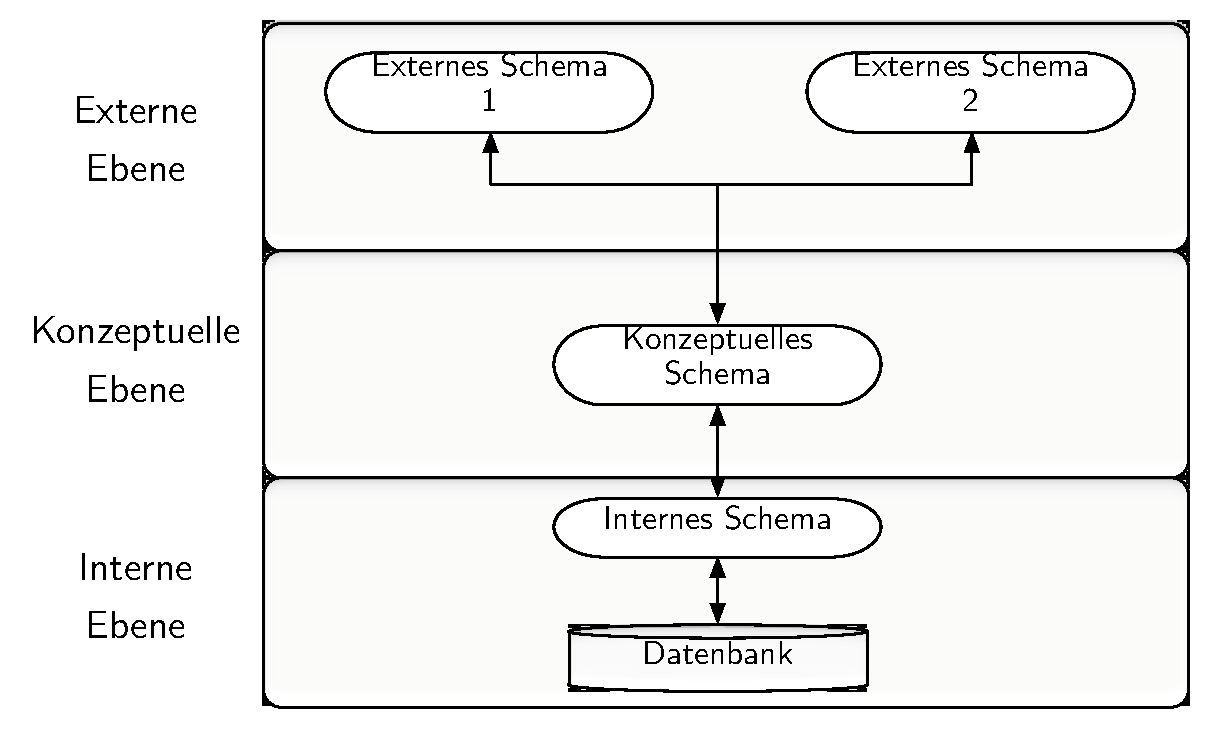
\includegraphics[scale=0.35]{img/ansisparc.pdf}
			\end{figure}
		\end{column}
		\begin{column}{.48\textwidth}
		\structure{ANSI/SPARC 3-Schicht-Architektur}
			\begin{itemize}
				\item Externe Ebene beschreibt Sichten auf die Daten
				\item Konzeptuelle Ebene beschreibt die system- und anwendungsunabhängige Struktur
				\item Interne Ebene beschreibt physische Speicherstrukturen einer Datenbank
			\end{itemize}
			\structure{Gewährleistung der logischen und physischen Datenunabhängigkeit}
		\end{column}
	\end{columns}
\end{frame}

\begin{frame}{\insertsection}
	\framesubtitle{\insertsubsection}
	\begin{block}{Physische Datenunabhängigkeit}
		\begin{itemize}
			\item Physische Speicherstrukturen werden verborgen
			\item Änderungen an der physischen Struktur haben keinen Einfluss auf die konzeptuelle Struktur
		\end{itemize}
	\end{block}

	\begin{block}{Logische Datenunabhängigkeit}
		\begin{itemize}
			\item Konzeptuelle Strukturen werden verdeckt
			\item Zugriff auf Daten über Sichten
			\item Änderungen an konzeptueller Struktur haben keinen Einfluss auf die Sichten
		\end{itemize}
	\end{block}
	\alert{Die logische Datenunabhängigkeit ist wesentlich schwerer zu erreichen als die physische und kann nur für einfachste 
		Modifikationen des Datenbankschemas gewährleistet werden!}
\end{frame}

\subsection{Generelle Architektur eines DBMS}
\begin{frame}{\insertsection}
	\framesubtitle{\insertsubsection}

	\begin{figure}
		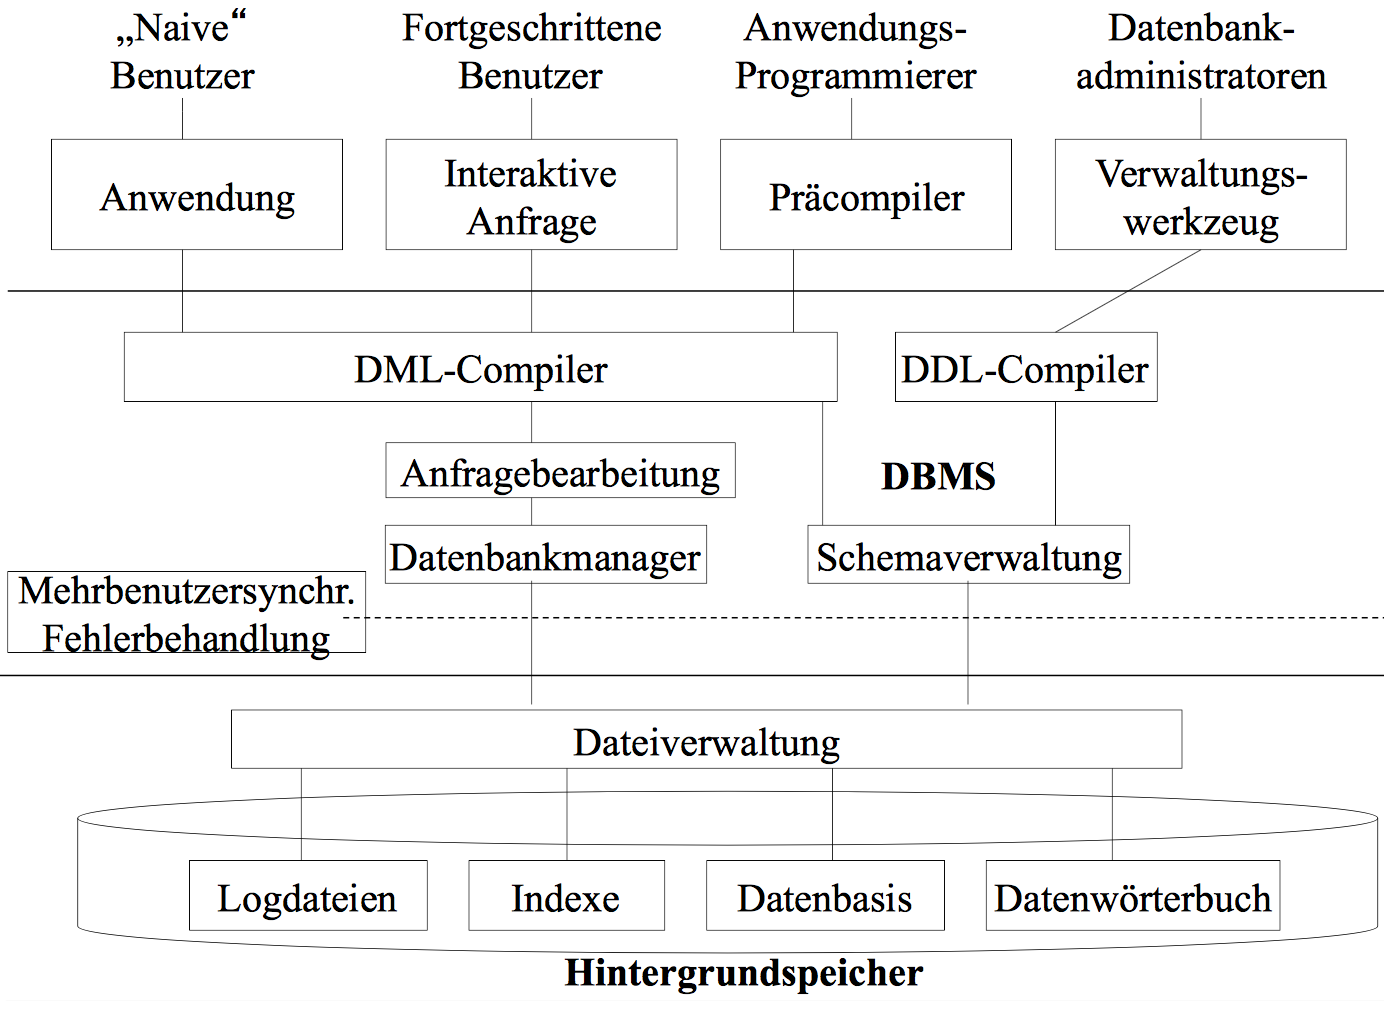
\includegraphics[scale=0.16]{img/db_arch.png}
		\caption{Architekturübersicht eines DBMS (vgl. \cite[S. 31]{KE15})}
	\end{figure}
\end{frame}

\begin{frame}{\insertsection}
	\framesubtitle{\insertsubsection}
	\structure{Vorteile bei der Nutzung eines DBMS:}
	\begin{itemize}
		\item Kontrolle über Redundanzen 
		\item Zugriffskontrolle der Benutzer \"uber Authentisierung und Autorisierung
		\item Persistenter Datenspeicher für Programmobjekte 
		\item Realisierung von Speicherstrukturen und effizienten Suchtechniken 
		\item Backup und Recovery 
		\item Ermöglichen eine Vielzahl von Benutzerschnittstellen 
		\item Repräsentieren komplexe Beziehungen entlang der Daten 
		\item Sicherstellung der referentiellen Integrität		
	\end{itemize}
	
\end{frame}

\section*{Übungsaufgaben}
%\subsection*{Grundlegendes Datenbankverständnis}
\begin{frame}{\insertsection}
	%\framesubtitle{\insertsubsection}
\begin{alertblock}{Grundlegendes Datenbankverständnis}
	\begin{enumerate}
		\item Benennen Sie die Problemstellungen dateibasierter Datenhaltung in einem Dateisystem. Erläutern Sie auch die Schwierigkeiten, die bei der Entwicklung dateibasierter Anwendungen existieren.
		\item Grenzen Sie die Begriffe \textit{Datenbank} und \textit{Datenbankmanagementsystem} voneinander ab.
		\item Erläutern Sie das ANSI/SPARC-Modell sowie die Begriffe \textit{logische} und \textit{physische} Datenunabhängigkeit.
		\item Beschreiben Sie die Vorteile beim Einsatz eines DBMS jeweils anhand eines Beispiels.
		\item Können Sie sich nachteilige Eigenschaften eines DBMS vorstellen, sodass ein DBMS in bestimmten Szenarien \textit{keinen} Einsatz finden sollte?
		\item Erläutern Sie die Komponenten der Datenbankarchitektur.
	\end{enumerate}
	\end{alertblock}
\end{frame}

%\section*{Zusammenfassung}
%\begin{frame}{Zusammenfassung}
%	\begin{itemize}
%		\item Anforderungen von Applikationen an die Datenhaltung
%		\item Historische Einordnung
%		\item Erläuterung der Problemstellungen dateibasierter Datenhaltung
%		\item Terminologien
%		\begin{itemize}
%			\item Datenbank und Datenbankmanagementsystem
%			\item Datenmodelle, Schemata und Datenbankzustand
%		\end{itemize}
%		\item ANSI/SPARC Architekturmodell
%		\item Datenbanksprachen
%		\item Beteiligte Akteure
%	\end{itemize}
%\end{frame}

%!TEX root = Slides.tex
\part{Datenbankentwurf und Datenmodelle}
\label{part:relmod}

\section{Datenbankentwurf}
\subsection{Generelles Vorgehen}

\begin{frame}{\insertsection}
\framesubtitle{\insertsubsection}
Datenbanken bilden einen Teil der realen Welt ab (Universe of Discourse) und sind logisch zusammenhängend. Sie beinhalten Daten, die einem vordefinierten Schema entsprechen: 
\begin{itemize}
	\item Objekte der realen Welt 
	\item Beziehungen zwischen den Objekten
	\item Nebenbedingungen
\end{itemize}

\begin{block}{Der Datenbank-Entwurfsprozess}
	\begin{itemize}
		\item Identifizierung der notwendigen Ausschnitte der realen Welt, die für die Abbildung eines Themengebietes notwendig sind
		\item Überführung dieses Ausschnittes in ein adäquates Datenbankschema.
	\end{itemize}
\end{block}
\end{frame}


\begin{frame}\frametitle{\insertsection}
%\framesubtitle{Generelles Vorgehen}
\alert{Im Datenbank-Entwurfsprozess müssen zwei Dinge strikt beachtet werden:}
\begin{enumerate}
\item Vermeidung von Redundanzen im Datenbestand. Mehrfache Speicherung einer Information führt zu Inkonsistenzen, fehlerhaften Datenbeständen
\item Vollständigkeit: Ein nicht vollständiges Datenmodell, welches Aspekte der realen Welt nur unzureichend bzw. zu stark vereinfacht abbildet, führt zu starken Einschränkungen in der späteren Verwendung der Anwendung.
\end{enumerate}

\begin{block}{Das Design einer Datenbank}
Es gibt nicht \textit{das eine} Datenbankdesign - vielmehr können unterschiedliche korrekte Datenbank-Designs existieren. 
Viele Wege führen nach Rom -- \textit{aber eben nicht alle!}
\end{block}
\end{frame}


\begin{frame}[t,label=dbentwurf]\frametitle{Datenbankentwurf}
%\framesubtitle{Generelles Vorgehen}

\begin{figure}
\begin{tikzpicture}
\node[align=center, drop shadow, black, rectangle, minimum width=3cm] (anforderung) {Anforderungs-\\Analyse}; 
\node[align=center, drop shadow, black, rectangle, minimum width=3cm] (konzept) [above right=0.2cm of anforderung] {Konzeptuelles\\Design}; 
\node[align=center, drop shadow, black, rectangle, minimum width=3cm] (logisch) [above right=0.2cm of konzept] {Logischer\\Entwurf}; 
\node[align=center, drop shadow, black, rectangle, minimum width=3cm] (physisch) [above right=0.2cm of logisch] {Physischer\\Entwurf}; 

\path[draw,-latex, thick] (anforderung.north) |- (konzept.west); 	
\path[draw,-latex, thick] (konzept.north) |- (logisch.west); 
\path[draw,-latex, thick] (logisch.north) |- (physisch.west); 

\end{tikzpicture}
\caption{Der Datenbank-Entwurfsprozess}
\end{figure}		
\end{frame}

\begin{frame}[t]\frametitle{\insertsection}
%\framesubtitle{Generelles Vorgehen}
\begin{itemize}
\item Anforderungsanalyse
\begin{itemize}
\item Gespräche mit Experten der Fachdomäne
\item Dokumentation der Anforderungen (Textdokumente, UML usw.)
\end{itemize}
\item Konzeptueller Entwurf
\begin{itemize}
\item Übersetzung der Anforderungen in ein konzeptuelles Modell
\item Output: ER-Diagramme
\end{itemize}
\item Logischer Entwurf
\begin{itemize}
\item Übersetzung des ER-Modells in ein implementierendes Datenmodell
\item Hier: das relationale Datenmodell
\end{itemize}
\item Physischer Entwurf
\begin{itemize}
\item Festlegung von Datei- und Index-Strukturen
\item $\Rightarrow$ Vorlesung \textit{Datenbanktechnik}
\end{itemize}
\end{itemize}
\end{frame}

\begin{frame}[t]\frametitle{Datenbankentwurf}
\framesubtitle{Beispiel}
\begin{block}{Anwendungsfall}
	Ihr Auftraggeber Kunde bittet Sie, eine Datenbank für die Verwaltung seiner Kunden zu entwerfen. 
	Zu jedem Kunden soll eine Kundennummer und der Name gespeichert werden.
\end{block}

\begin{itemize}
	\item Der Ausschnitt der realen Welt besteht in diesem Fall aus \textit{Kunden}. 
	\item Jeder Kunde besitzt zusätzliche Eigenschaften bzw. \textit{Attribute}, z.B. eine Kundennummer und ein Name.
\end{itemize}
\abs
\alert{Nachdem Sie die Anforderungen aufgenommen haben, können Sie sich nun an den Entwurf der Datenbank begeben.}
\end{frame}

\section{Datenmodelle}

\begin{frame}{\insertsection}
\structure{Datenmodelle beschreiben Daten, deren Beziehungen, Darstellungen, Bedeutung sowie Konsistenz- und Integri\"atsbedingungen}
\abs
\structure{Datenmodelle befinden sich auf unterschiedlichen Abstraktionsebenen:}
\newline
\structure{Modelltypen:}
\begin{description}[leftmargin=0cm]
\item[\textbf{konzeptionell:}] technologieneutral; Abbild der betriebswirtschaftlichen Realität
\begin{itemize}
	\item Vertreter: Entity-Relationship-Modell, objektorientiertes Entwurfsmodell
\end{itemize}
\item[\textbf{logisch:}] technologieneutral; formal, für bestimmte Datenhaltungssysteme, zur Implementierung 
\begin{itemize}
	\item Vertreter: Relationales Modell, objektorientierte Modelle, 
	Netzwerk- und Hierarchie-Datenmodell (veraltet) …
\end{itemize}
\item[\textbf{physisch:}] technologiespezifisch; beschreiben Speicherung, Zugriff, Datentypen
datenbanksystemabh\"angig; oft proprietär
\end{description}
\end{frame}

\section{Entity-Relationship-Modell}\label{erm}
%\subsection{Grundlagen}

\begin{frame}{\insertsection}
%\framesubtitle{\insertsubsection}
\structure{Konzeptionelles, semantisches Modell bestehend aus Entit\"aten, Beziehungen, Attributen:}
\begin{itemize}
	\item Entit\"aten	repr\"asentieren abstrakte oder physische Objekte der realen Welt
	\begin{itemize}
		\item physisch: Autos, Personen, Geb\"aude
		\item abstrakt: Firma, Handel, Beruf
	\end{itemize}
	\item Beziehungen beschreiben Zusammenh\"ange zwischen zwei oder mehreren Entit\"aten
	\item Attribute beschreiben Eigenschaften von Entit\"aten und Beziehungen
\end{itemize}
\end{frame}

\begin{frame}{\insertsection}
%\framesubtitle{\insertsubsection}
\structure{.. basierend auf Typen:}
\begin{itemize}
	\item Entit\"atstyp beschreibt alle Entit\"aten dieses Typs
	\begin{itemize}
		\item Entit\"aten: Instanzen des Entit\"atstyps
		\item Entit\"atsmenge (entity set): Menge der betreffenden Entit\"aten dieses Typs
  \end{itemize}
	\item Beziehungstyp beschreibt Zusammenhang zwischen zwei oder mehreren Entit\"atstypen
	\item Attribute
	\begin{itemize}
		\item Eigenschaften von Entit\"ats- und Beziehungstypen
		\item Eigenschaften einzelner Entit\"aten und Beziehungen werden durch die Attributwerte festgelegt 
	\end{itemize}
\end{itemize}
\end{frame}

\begin{frame}{\insertsection}
%\framesubtitle{\insertsubsection}
 \structure{Beispiel}
 \begin{itemize}
	\item Entit\"atstyp \emph{Professor}: Alle Personen (Entit\"aten) vom Typ \emph{Professor}
	\begin{itemize}
		\item Attribute \emph{ID} und \emph{Name}
	\end{itemize}
	\item Entit\"atstyp \emph{Fach}: Alle Unterrichtseinheiten (Entit\"aten) vom Typ \emph{Fach}
	\begin{itemize}
	 \item Attribute \emph{FachNr} und \emph{Name}
  \end{itemize}
	
	\item Beziehungstyp \emph{Lehre}: Zuordnung von \emph{Professor} und \emph{Fach} 
 \end{itemize}
\end{frame}

\begin{frame}{\insertsection}
\framesubtitle{Mengentheoretische Sicht}
\structure{Entit\"atstyp $\equiv$ Entit\"atsmenge}
	\begin{figure}
		Entit\"atstyp \emph{Professor} $\Rightarrow$\quad 
		\begin{minipage}{0.3\linewidth}
			\centering
			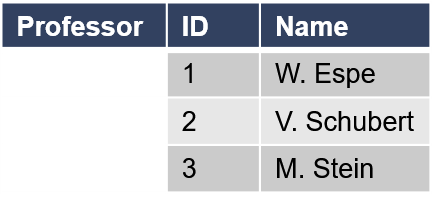
\includegraphics[scale=0.5]{img/ERM-BeispielEntitaetsmengeProfessor.png}
		\end{minipage}
	  \quad Entit\"atsmenge f\"ur \emph{Professor}
	\end{figure}    
	\begin{figure}
  	Entit\"atstyp \emph{Fach} $\Rightarrow$\quad 
	  \begin{minipage}{0.3\linewidth}
		 \centering
		 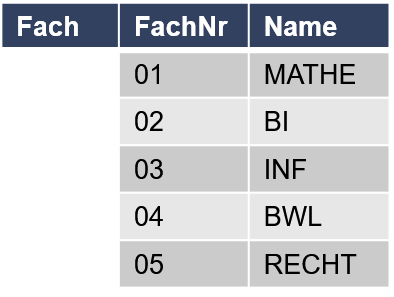
\includegraphics[scale=0.5]{img/ERM-BeispielEntitaetsmengeFach.png}
	  \end{minipage}
	  \quad Entit\"atsmenge f\"ur \emph{Fach}
  \end{figure}    
\end{frame}

\begin{frame}{\insertsection}
\framesubtitle{Mengentheoretische Sicht}
\structure{Beziehungstyp $\equiv$ Relation zwischen Entit\"atsmengen (mit Semantik angereichert)}
	\begin{figure}
		Beziehungstyp \emph{Lehre} $\Rightarrow$
		\begin{minipage}{0.4\linewidth}    	
 	    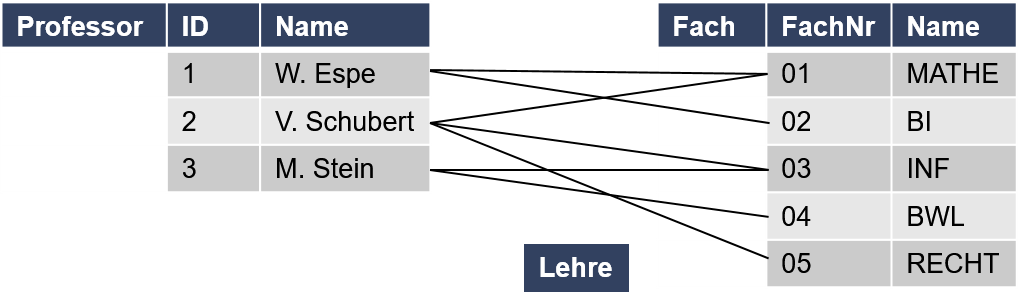
\includegraphics[scale=0.35]{img/ERM-BeispielRelationLehreProfessorFach.png}
 	  \end{minipage} 
    \quad Relation f\"ur \emph{Lehre}
 	\end{figure}    
\end{frame}

\begin{frame}{\insertsection}
\framesubtitle{Mengentheoretische Sicht -- Wiederholung Mengenlehre}
\begin{itemize}
 \item Eine (endliche) \emph{Menge} $M$ besteht aus \emph{Elementen} $e_1$, $e_2$, $\ldots$, $e_m$
   \begin{itemize}
	   \item Bezeichnung: $M=\{e_1, e_2,\ldots , e_m\}$
	 \end{itemize}
 \item Jedes Element $e_i$ f\"ur $i= 1, 2,\ldots,m$ geh\"ort zu der Menge $M$
   \begin{itemize}
   	\item Bezeichnung: $e_i\in M$
   \end{itemize}
 \item Die \emph{M\"achtigkeit} $\vert M\vert$ einer (endlichen) Menge $M$ ist die Anzahl der Elemente von $M$.
\end{itemize}
\onslide\pause 
\abs\abs
\structure{\textbf{Wichtige Eigenschaften von Mengen:}}
\begin{itemize}
	\item In einer Menge existieren keine doppelten Elemente
	\item Die Elemente einer Menge sind nicht geordnet
\end{itemize}
\end{frame}

\begin{frame}{\insertsection}
\framesubtitle{Mengentheoretische Sicht -- Wiederholung Mengenlehre}
\begin{itemize}
	\onslide 
	\item Ein Element $e$ kann zu zwei Mengen $M_1$ und $M_2$ geh\"oren: $e\in M_1$ und $e\in M_2$\\[4pt]	
	\pause 
	\item Die Menge aller Elemente, die zu $M_1$ und $M_2$ geh\"oren bilden wieder eine Menge, die sogenannte \emph{Schnittmenge} 
	$M_1\cap M_2$
	\begin{equation*}
	M_1\cap M_2=\{ e\mid e\in M_1\text{ und } e\in M_2\}
	\end{equation*}
	\pause
	\item Die Menge aller Elemente, die zu $M_1$ oder zu $M_2$ geh\"oren bilden wieder eine Menge, die sogenannte \emph{Vereinigungsmenge}
	$M_1\cup M_2$
	\begin{equation*}
	M_1\cup M_2=\{ e\mid e\in M_1\text{ oder } e\in M_2\}
	\end{equation*}
\end{itemize}
\end{frame}

\begin{frame}{\insertsection}
\framesubtitle{Mengentheoretische Sicht -- Wiederholung Mengenlehre}
\begin{itemize}
\onslide 
\item Ist $M$ eine Menge, deren Elemente zu $N$ geh\"oren, dann hei\ss t $M$ \emph{Untermenge} von $N$.\\[4pt]
Bezeichnung: $M\subseteq N$\\[8pt]
\pause
\item Gilt $M\subseteq N$ und $N\subseteq M$, dann folgt daraus $M=N$.\\[8pt]
\pause
\item
Die Menge aller Elemente von $M_2$, die nicht zu der Menge $M_1$ geh\"oren, hei\ss t die Differenz von $M_2$ und $M_1$.\\[4pt]
Bezeichnung: $M_2 - M_1$\\[8pt]
\pause
\item Es gilt: $M\cap N = M - (M - N) = N- (N - M)$ (\"Ubungsaufgabe!)
\end{itemize}
\end{frame}

\begin{frame}{\insertsection}
\framesubtitle{Mengentheoretische Sicht -- Wiederholung Mengenlehre}
\begin{definition}[Funktion]
\begin{enumerate}
	\item 
	Seien $M_1$ und $M_2$ zwei Mengen. Eine Funktion $f:M_1\to M_2$ ist eine eindeutige Zuordnung von Elementen 
	aus $M_1$ auf Elemente aus $M_2$. Das hei\ss t, jedem $x\in M_1$ wird genau ein $y\in M_2$ zugeordnet. 
	\\[4pt]
	Bezeichnung: $x\overset{f}{\mapsto} y$ oder $y=f(x)$.
	\\[4pt]
	\item Zwei Funktionen $f,g:M_1\to M_2$ sind gleich, falls $f(x)=g(x)$ f\"ur jedes $x\in M_1$ gilt. 
	\\[4pt]
	Bezeichnung: $f=g$.
\end{enumerate}
\end{definition}
\end{frame}

\begin{frame}{\insertsection}
\framesubtitle{Mengentheoretische Sicht -- Wiederholung Mengenlehre}
\begin{itemize}
	\onslide
	\item Für zwei (endliche) Mengen $M_1=\{e_1, e_2,\ldots , e_n\}$ und $M_2=\{c_1, c_2, \ldots , c_m\}$ kann man das \emph{kartesische Produkt} 
	$M_1\times M_2$ bilden:
	\begin{itemize} 
		\item Das kartesische Produkt $M_1\times M_2$ ist die Menge aller Tupel $(e_i,c_j)$ mit $e_i\in M_1$ und $c_j\in M_2$.
		\item Das hei\ss t
		\begin{equation*}
		M_1\times M_2=\{(e_1,c_1), (e_1,c_2),\ldots, (e_1,c_m),(e_2,c_1), \ldots, (e_n,c_m)\}
		\end{equation*}
	\end{itemize}
  \pause
	\item Entsprechend kann man aus $r$ (endlichen) Mengen $M_1$, $M_2$, $\ldots$, $M_r$ das $r$-fache kartesische Produkt 
	$M_1\times M_2 \times \cdots \times M_r$ aller $r$-Tupel bilden:
	\begin{equation*}
	\begin{split}
	M_1\times M_2 \times \cdots \times M_r &=\{(e_1,c_1, \ldots, x_1), (e_1,c_1,\ldots, x_2),\ldots, (e_n,c_m, \ldots, x_p)\}\\
	&=\{\underbrace{(e,c,\ldots,x)}_\text{r-Tupel} \mid e\in M_1, c\in M_2,\ldots ,x\in M_r\}
	\end{split} 
	\end{equation*} 
\end{itemize}
\end{frame}

\begin{frame}{\insertsection}
\framesubtitle{Mengentheoretische Sicht -- Relationen}
\begin{definition}[Zweistellige Relationen]
	Seien $M_1$ und $M_2$ Mengen. Eine zweistellige Relation $R$ ist eine Teilmenge des kartesischen Produktes $M_1\times M_2$.
\begin{equation*} 
R \subseteq M_1 \times M_2
\end{equation*} 
\end{definition}
\abs 
Es gilt: $\vert M_1\times M_2\vert = \vert M_1\vert\cdot \vert M_2\vert$
\abs\abs
\alert{Beispiele!}
\end{frame}

\begin{frame}{\insertsection}
\framesubtitle{Mengentheoretische Sicht -- Relationen}
\begin{definition}[r-stellige Relationen]
Seien $M_1$, $M_2$, $\ldots$, $M_r$ Mengen. Eine $r$-stellige Relation $R$ ist eine Teilmenge des $r$-fachen 
kartesischen Produktes $M_1 \times M_2 \times \cdots \times M_r$.
\begin{equation*} 
R \subseteq M_1 \times M_2 \times \cdots \times M_r
\end{equation*} 
\end{definition}
\abs 
Es gilt: $\vert M_1\times \ldots \times M_r\vert = \vert M_1\vert\cdot\ldots\cdot \vert M_r\vert =\prod_{i=1}^r\vert M_i\vert$
\abs\abs
\alert{Beispiele!}
\end{frame}

\begin{frame}{\insertsection}
\framesubtitle{Mengentheoretische Sicht -- Zur"uck zum Beispiel}
\centering 
\begin{minipage}[c]{0.3\linewidth}
	\begin{figure} 
		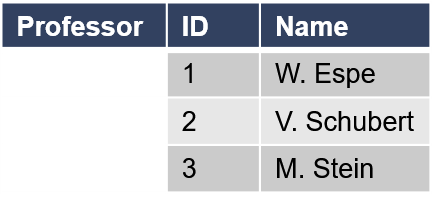
\includegraphics[scale=0.45]{img/ERM-BeispielEntitaetsmengeProfessor.png}
	\end{figure}
\end{minipage}
\begin{minipage}[c]{0.5\linewidth}
	\begin{equation*}
	\begin{split} 
	&\text{Entit\"atsmenge f\"ur \emph{Professor}}\\
	&=\{e_{P(1, \text{Espe})},e_{P(2,\text{Schubert})},e_{P(3, \text{Stein})}\}
	\end{split}
	\end{equation*}
\end{minipage}
\abs\abs\abs 
\begin{minipage}[c]{0.3\linewidth}
	\begin{figure} 
		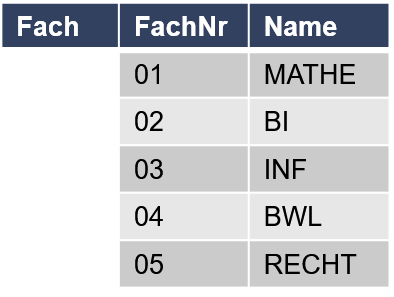
\includegraphics[scale=0.45]{img/ERM-BeispielEntitaetsmengeFach.png}
	\end{figure}
\end{minipage}
\begin{minipage}[c]{0.5\linewidth}
	\begin{equation*}
	\begin{split} 
	&\text{Entit\"atsmenge f\"ur \emph{Fach}}\\
	&=\{e_{F(01,\text{MATHE})},e_{F(02,\text{BI})},\\
	&\quad\,\,\,\, e_{F(03,\text{INF})},e_{F(04,\text{BWL})},e_{F(05,\text{RECHT})}\}
	\end{split}
	\end{equation*}
\end{minipage}
\end{frame} 

\begin{frame}{\insertsection}
\framesubtitle{Mengentheoretische Sicht -- Zur"uck zum Beispiel}
\centering 
\begin{minipage}[c]{0.5\linewidth}
\begin{figure} 
	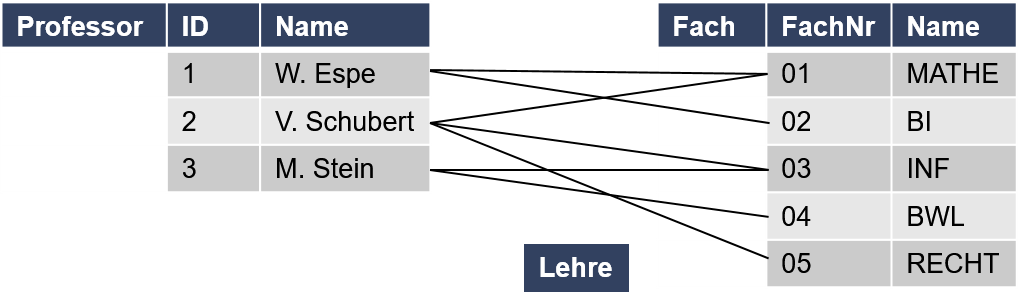
\includegraphics[scale=0.45]{img/ERM-BeispielRelationLehreProfessorFach.png}
\end{figure}
\end{minipage}
\abs 
\begin{minipage}[c]{0.5\linewidth}
\begin{equation*}
\begin{split} 
&\text{Relation f\"ur \emph{Lehre}}\\
&=\{(e_{P(1, \text{Espe})}, e_{F(01,\text{MATHE})}),(e_{P(1, \text{Espe})}, e_{F(02,\text{BI})}),\\
&\quad\,\,\,\,(e_{P(2,\text{Schubert})}, e_{F(01,\text{MATHE})}),(e_{P(2,\text{Schubert})}, e_{F(03,\text{INF})}),\\
&\quad\,\,\,\,(e_{P(2,\text{Schubert})}, e_{F(05,\text{RECHT})}),(e_{P(3, \text{Stein})}, e_{F(03,\text{INF})}),\\
&\quad\,\,\,\,(e_{P(3, \text{Stein})}, e_{F(04,\text{BWL})})\}
\end{split}
\end{equation*}
\end{minipage}
\end{frame} 

\begin{frame}{\insertsection}
\framesubtitle{Mengentheoretische Sicht}
\begin{itemize}
	\item Seien $E_1$, $E_2$, $\ldots$, $E_r$ Entit\"atstypen und $\mathcal{M}(E_1)$, $\mathcal{M}(E_2)$, $\ldots$, $\mathcal{M}(E_r)$ 
	die zugeh\"origen Entit\"atsmengen.
	\item Sei $B$ der Beziehungstyp zwischen den Entit\"aten $E_1$, $E_2$, $\ldots$, $E_r$. 
	Dann bezeichnet $\mathcal{R}(B)$ die zugeh\"orige Relation. 
	\begin{equation*} 
	\mathcal{R}(B)\subseteq	\mathcal{M}(E_1)\times\mathcal{M}(E_2)\times\cdots\times\mathcal{M}(E_r)
	\end{equation*} 
\end{itemize}
\end{frame} 

\begin{frame}{\insertsection}
%\framesubtitle{\insertsubsection}
\structure{Graphische Notation}
\newline
\begin{itemize}
	\item Entit\"atstypen: Rechtecke mit Namen des Entit\"atstyps
		\begin{figure}
			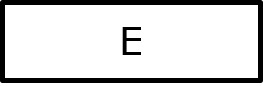
\includegraphics[scale=0.5]{img/ERM-EntitaetTyp.png}
		\end{figure}
	\item Beziehungstypen: Rauten mit Namen des Beziehungstyps
		\begin{figure}
			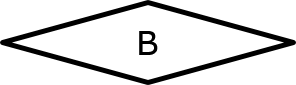
\includegraphics[scale=0.5]{img/ERM-BeziehungTyp.png}
		\end{figure}
	\item Attribute: Ovale mit Namen des Attributs
	  \begin{figure}
	  	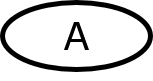
\includegraphics[scale=0.5]{img/ERM-AttributTyp.png}
  	\end{figure}
\end{itemize}
\end{frame}

\begin{frame}{\insertsection}
%\framesubtitle{\insertsubsection}
\structure{Graphische Notation}
\begin{itemize}
	\item Entit\"atstypen durch Linien mit Beziehungstypen verbunden
	\begin{figure}
		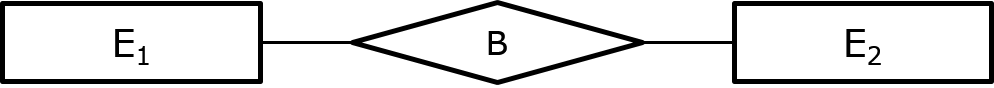
\includegraphics[scale=0.5]{img/ERM-EntitaetRelationTyp.png}
	\end{figure}  
	\item Entit\"ats- und Beziehungstypen durch Linien mit Attributen verbunden
	\begin{figure}
	 \centering
	 \begin{minipage}{0.3\linewidth}
		\centering
		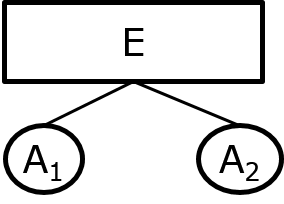
\includegraphics[scale=0.5]{img/ERM-EntitaetAttributTyp.png}
	 \end{minipage}
 	 \begin{minipage}{0.3\linewidth}
		\centering
		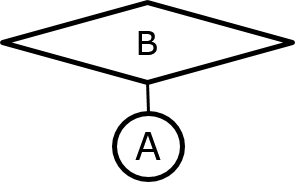
\includegraphics[scale=0.5]{img/ERM-RelationAttributTyp.png}
   \end{minipage}
	\end{figure}    
\end{itemize}
\end{frame}

\begin{frame}{\insertsection}
%\framesubtitle{\insertsubsection}
\structure{Graphische Notation -- Beispiel}
\begin{itemize}
	\item Entit\"atstypen
 	 \begin{figure}
		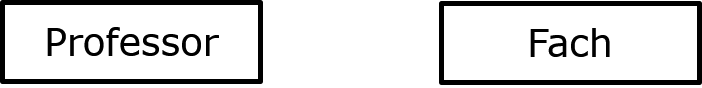
\includegraphics[scale=0.5]{img/ERM-BeispielEntitaetTyp.png}
	 \end{figure}  
	\item Beziehung der beiden Entit\"atstypen
	 \begin{figure}
	  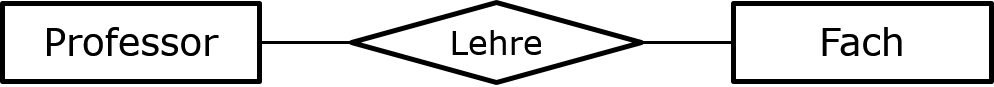
\includegraphics[scale=0.5]{img/ERM-BeispielEntitaetRelationTyp.png}
   \end{figure}  
 \item ... attributiert
  \begin{figure}
	 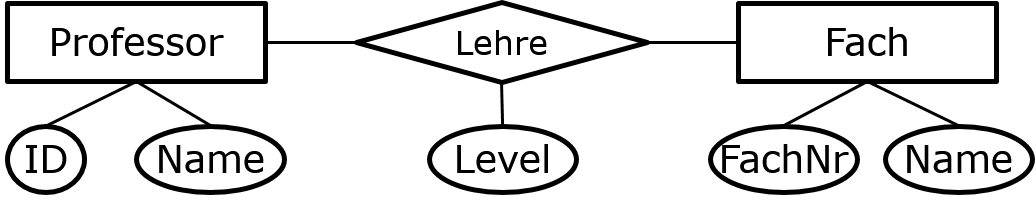
\includegraphics[scale=0.5]{img/ERM-BeispielEntitaetRelationAttributTyp.png}
  \end{figure}  
\end{itemize}
\end{frame}

\begin{frame}{\insertsection}
\framesubtitle{Noch ein Beispiel}
\begin{columns}
	\begin{column}{.31\textwidth}
		\begin{figure}
			\begin{tikzpicture}[node distance=7em]
			\node[entity] (Kunde) {\small Kunde}; 
			\node[attribute] (knr) [above left of=Kunde] {{\small KNR}} edge (Kunde); 
			\node[attribute] (name) [above of=Kunde] {\small Name} edge (Kunde); 
			\end{tikzpicture}
			\caption{Entit\"atstyp}
		\end{figure}		
	\end{column}
	
	\begin{column}{.31\textwidth}
		\begin{figure}
			\begin{tabbing}
				\textbf{Kunde} \= Name \= \kill
				\textbf{Kunde:}\\
				KNR \> 1 \\
				Name \> Mustermann \\
			\end{tabbing}
			\caption{Entit\"at}
		\end{figure} 
	\end{column}
	
	\begin{column}{.31\textwidth}
		\begin{figure}
			\begin{tabular}{|c|c|}\hline
				\multicolumn{2}{|c|}{\small \textbf{Kunde}}\\\hline\hline
				\small \textbf{KNR} & \small \textbf{Name} \\\hline 
				\small 1 &\small Mustermann \\\hline 
				\small 2 & \small Musterfrau \\\hline 
				$\cdots$ & $\cdots$ \\\hline
			\end{tabular}				
			\caption{Entit\"atsmenge}
		\end{figure} 
	\end{column}
\end{columns}
% \alert{Wertebereiche / Domänen werden in ER-Diagrammen nicht festgehalten!}
\end{frame}

\begin{frame}{\insertsection}
\framesubtitle{Grad einer Beziehung}
\begin{definition}[Grad von Beziehungen]
	\label{def:gradVonBeziehungen}
	Der \textit{Grad} einer Beziehung ist die Anzahl der an der Beziehung teilnehmenden Entit\"atstypen.
\end{definition}
\begin{itemize}
	\item Beziehungen vom Grad 2 bezeichnet man als \textit{binäre} Beziehungen
	\item Beziehungen vom Grad 3 bezeichnet man als \textit{ternäre} Beziehungen
	\item Beziehungen vom Grad n bezeichnet man als $n$\textit{-äre} Beziehungen
\end{itemize}
\end{frame}

\begin{frame}[t]{\insertsection}
\framesubtitle{Rekursive Beziehungen}
\begin{itemize}
\item Rekursive Beziehungen sind erlaubt
\item Jeder Entitätstyp, der an einer Beziehung teilnimmt, spielt eine bestimmte Rolle.
\end{itemize}
\begin{figure}
	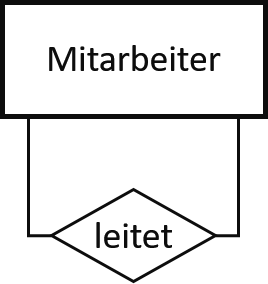
\includegraphics[scale=0.5]{img/ERM-Rekursiv.png}	
%  \begin{tikzpicture}[node distance=2em]
%   \node[entity] (ma) {\small Mitarbeiter}; 
%   \node[relationship] (leitet) [below=of ma] {\small{leitet}}; 
%   \draw (ma.west) |- (leitet.west) node[midway,above,rotate=90, xshift=10mm] {\tiny Vorgesetzter}; 
%   \draw (ma.east) |- (leitet.east) node[midway,below,rotate=90, xshift=10mm] {\tiny Angestellter};  			
%   \end{tikzpicture}
   \caption{Rekursive Beziehung}
\end{figure}		
\end{frame}

\begin{frame}[t]{\insertsection}
\framesubtitle{Attributarten}
\structure{Mehrere Attributtypen kommen in ER-Diagrammen vor:}
\onslide
\begin{itemize}
	\item Atomare Attribute, die nicht geteilt werden können (z.B. Alter, Postleitzahl, Nachname)
	\item Zusammengesetzte Attribute (z.B. das Attribut \textit{Anschrift}, welches aus weiteren Attributen
	PLZ, Ort und Straße zusammengesetzt ist)
	\pause
	\item Einwertige Attribute, bei denen zu einem bestimmten Zeitpunkt \textit{genau ein Wert} existiert 
	\item Mehrwertige Attribute, bei denen zu einem bestimmten Zeitpunkt mehrere Werte existieren können (z.B. wenn eine Person zwei akademische Titel hat)
	\pause
	\item Abgeleitete Attribute, deren Wert sich aus anderen Attributen herleiten lässt (z.B. kann ein Attribut \textit{Alter} aus dem Geburtsdatum errechnet werden)
\end{itemize}
\pause
\abs
\structure{\texttt{null}-Eigenschaft:}
\begin{itemize}
	\item \texttt{null}-Attribute sind Attribute, die f\"ur manche Entitäten nicht belegt sind. 
	\begin{itemize}
		\item \alert{Achtung: \texttt{null}-Attribute bergen Interpretationsspielraum!} 
	\end{itemize}
\end{itemize}
\end{frame}

\begin{frame}{\insertsection}
\framesubtitle{Attributtypen -- Graphische Notation}
\begin{figure}
\begin{tikzpicture}[node distance=7em]
\node[attribute] (einfach) {\small Einfach}; 
\node[derived attribute] (abgeleitet) [right=of einfach] {\small Abgeleitet} ; 
\node[multi attribute] (multi) [right=of abgeleitet] {\small Mehrwertig} ;
\node[attribute, align=center] (zusammen) [below=0.5cm of abgeleitet] {\small Zusammengesetzt\\Ort};
\node[attribute] (plz) [below left=3em of zusammen] {\small PLZ} edge (zusammen); 
\node[attribute] (str) [below right=3em of zusammen] {\small Str} edge (zusammen); 
\end{tikzpicture}
\caption{Attributtypen}
\end{figure}		
\end{frame}

\begin{frame}[t]{\insertsection}
\framesubtitle{Identifizierbarkeit von Entitäten}
\begin{definition}[Schlüssel]
Ein Schlüssel ist ein Attribut oder eine Attributkombination, mit dem eine Entität eines Entitätstyps eindeutig identifiziert 
werden kann.\label{def:er:key}
\end{definition}
\onslide\pause
\abs
Ein Schlüsselattribut wird durch Unterstreichung gekennzeichnet. Falls notwendig kann ein 
künstliches Schlüsselattribut (Surrogatschlüssel) zugefügt werden.
\begin{figure}
\begin{tikzpicture}[node distance=1em]
\node[entity] (Kunde) {\small Kunde}; 
\node[attribute] (knr) [above left=1em of Kunde] {\key{\small KNR}} edge (Kunde); 
\node[attribute] (name) [above right=1em of Kunde] {\small Name} edge (Kunde); 
\end{tikzpicture}
\caption{Entitätstyp mit Schlüsselattribut KNR}
\end{figure}		
\end{frame}

%\begin{frame}[t]{\insertsection}
%\framesubtitle{Noch ein Beispiel}
%\begin{figure}
%	\begin{tikzpicture}[node distance=2em]
%	\node[entity] (Student) {\small Student}; 
%	\node[attribute] (knr) [above left=2em of Student] {\key{\small MNR}} edge (Student); 
%	\node[attribute] (name) [above=2em of Student] {\small Name} edge (Student);
%	\node[relationship] (betreut) [right=of Student] {\small{betreut}} edge (Student); 
%	\node[entity] (prof) [right=of betreut]  {\small{Professor}} edge (betreut);
%	\node[attribute] (profnr) [above=of prof] {\small{\key{ProfNr}}} edge (prof);
%	\node[attribute] (profname) [above right=of prof] {\small{Name}} edge (prof);
%	\end{tikzpicture}
%	%	\caption{Beziehungstyp zwischen Entitätstypen}
%\end{figure}		
%\abs\alert{Achtung: Es gibt keine explizit vorgegebene Leserichtung!}
%\end{frame}

\begin{frame}[t]{\insertsection}
\framesubtitle{Noch ein Beispiel}
Abbildung \ref{er:attrel} drückt das Schreiben von Klausuren an einem bestimmten Datum aus.
\begin{figure}
	\begin{tikzpicture}[node distance=2em]
	\node[entity] (Student) {\small Student}; 
	\node[attribute] (knr) [above left=2em of Student] {\key{\small MNR}} edge (Student); 
	\node[attribute] (name) [above=2em of Student] {\small Name} edge (Student);
	\node[relationship] (schreibt) [right=of Student] {\small{schreibt}} edge node[auto,swap] {} (Student); 
	\node[entity] (klausur) [right=of schreibt]  {\small{Klausur}} edge node[auto,swap] {} (schreibt); 
	\node[attribute] (datum)[above=of schreibt] {\small{Datum}} edge (schreibt); 
	\node[attribute] (knr) [above=of klausur] {\small{\key{KNr}}} edge (klausur);
	\node[attribute] (kname) [above right=of klausur] {\small{Fach}} edge (klausur);
	\end{tikzpicture}
	\caption{\label{er:attrel}ER-Diagramm mit attributierter Beziehung}
\end{figure}		
\alert{Zu beachten: Es gibt keine explizit vorgegebene Leserichtung! Das ist implizite Semantik.}
\end{frame}

\begin{frame}{\insertsection}
\framesubtitle{Kardinalit\"aten -- Motivation}
\begin{itemize}
	\item Eine Person kann \textbf{keines}, \textbf{eines} oder \textbf{mehrere} \underline{Autos} besitzen
	\item Eine Person ist mit \textbf{keiner} oder \textbf{einer} \underline{Person} verheiratet
  \item Eine Person besitzt \textbf{einen} \underline{Ausweis}
	\item Ein Professor an einer Fakult\"at liest \textbf{keine}, \textbf{eine} oder \textbf{mehrere} \underline{Vorlesungen}
	\item Eine Vorlesung in einer Fakult\"at wird von \textbf{einem} oder \textbf{mehreren} \underline{Professoren} gelesen	
\end{itemize}
\end{frame}

%
% Chen-UML-Notation
%
\begin{frame}{\insertsection}
\framesubtitle{Kardinalit\"aten}
\begin{definition}[look-across-Kardinalit\"at]\label{carddef}
	Seien $E_1$, $E_2$, $\ldots$, $E_n$ Entit\"atstypen und $B$ ein Beziehungstyp zwischen diesen 
	Entit\"aten. 
	\abs
	Die Kardinalit\"at $C_i$ des Entit\"atstyps $E_i$ ($i\in\{1,\ldots,n\}$) gibt an, mit wie vielen 
	Entit\"aten des Typs $E_i$ ein vorgegebenes Tupel $(e_1,\ldots,e_{i-1},e_{i+1},\ldots,e_n)$ 	
	aus Entit\"aten der anderen Entit\"atstypen in Beziehung stehen kann.
\end{definition}
\abs\onslide\pause 
Es gibt unter anderem die Kardinalit\"aten $'1'$, $'n'$, $'0..1'$, $'0..n'$:
\begin{description}[leftmargin=0cm]
	\item[$1$:] Mit genau einer Entit\"at steht das vorgegebene Tupel in Beziehung.
	\item[$n$:] Mit einer oder mehreren Entit\"aten steht das vorgegebene Tupel in Beziehung.
	\item[$0..1$:] Mit keiner oder einer Entit\"at steht das vorgegebene Tupel in Beziehung.
	\item[$0..n$:] Mit keiner, einer oder mehreren Entit\"aten steht das vorgegebene Tupel in Beziehung.
\end{description}
\end{frame}

\begin{frame}{\insertsection}
\framesubtitle{Kardinalit\"aten -- Graphische Notation}
\begin{itemize}
	\item Kardinalit\"at $C_i$ von Entit\"atstyp $E_i$ in Beziehung $B$
\end{itemize}
\begin{figure}
	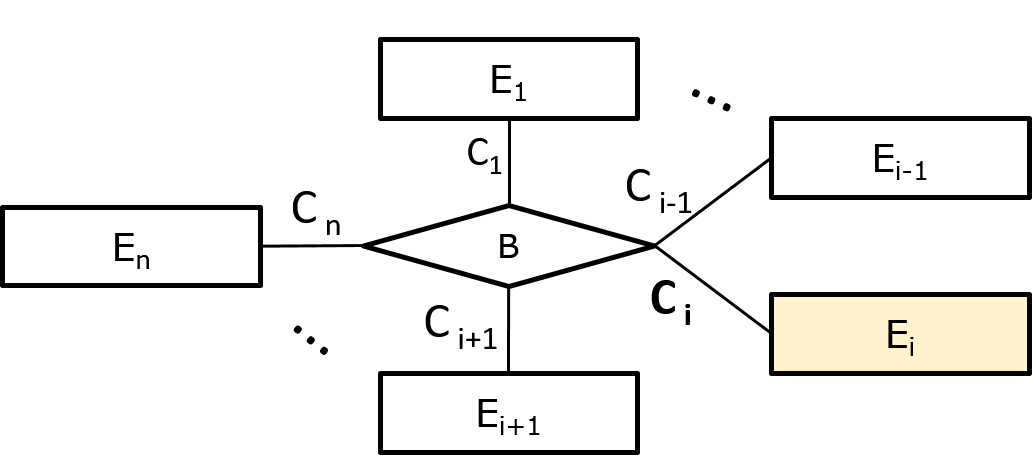
\includegraphics[scale=0.5]{img/ERM-Kardinalitaet.png}
\end{figure}  
% \alert{Machen Sie sich die Definition \ref{carddef} anhand von Beispielen klar.}
\end{frame}

\begin{frame}{\insertsection}
\framesubtitle{Kardinalit\"aten}
\begin{block}{Kardinalit\"aten anhand von Beispielen}
	\begin{description}[leftmargin=0cm]
		\item[1:n] Eine Person besitzt eines oder mehrere Autos. Jedes Auto wird von genau  
		einer Person besessen. Zwischen den Entit\"atstypen Person und Auto besteht ein [1:n]-Beziehungstyp.
		\item[n:m] Eine Person arbeitet an einem oder mehreren Projekten. Jedes Projekt wird durch 
		eine oder mehrere Personen bearbeitet.
		\item[1:1] Eine Person besitzt genau einen Ausweis und ein Ausweis geh\"ort zu genau einer Person. 
		\item[0..n\,:\,1] Ein Mitarbeiter besitzt genau einen Angestelltenstatus. Ein Angestelltenstatus geh\"ort zu keinem, einem 
		oder mehreren Mitarbeitern.
	\end{description}
\end{block}
 \alert{Zeichnen Sie die entsprechenden ERM-Diagramme.}
\end{frame}

\begin{frame}[t]{\insertsection}
\framesubtitle{Kardinalitäten}
\begin{figure}
	\begin{tikzpicture}[node distance=2em]
	\node[entity] (Student) {\small Student}; 
	\node[attribute] (knr) [above left=2em of Student] {\key{\small MNR}} edge (Student); 
	\node[attribute] (name) [above=2em of Student] {\small Name} edge (Student);
	\node[relationship] (betreut) [right=of Student] {\small{betreut}} edge node[auto,swap] {n} (Student); 
	\node[entity] (prof) [right=of betreut]  {\small{Professor}} edge node[auto,swap] {1} (betreut);
	\node[attribute] (profnr) [above=of prof] {\small{\key{ProfNr}}} edge (prof);
	\node[attribute] (profname) [above right=of prof] {\small{Fach}} edge (prof);
	\end{tikzpicture}
	\caption{ER-Diagramm mit Kardinalitäten}
\end{figure}		
 \alert{Was sagt dieses ERM-Diagramm aus?}
\end{frame}

\begin{frame}{\insertsection}
\framesubtitle{Kardinalitäten auf Entit\"atsmengen und Relationen}
\structure{[1:1]-Beziehung}
\newline 
(E) 1: Ordnet einer gegebenen Entit\"at $f_j \in F$ genau eine Entit\"at in $E$ zu. 
\newline 
(F) 1: Ordnet einer gegebenen Entit\"at $e_i \in E$ genau eine Entit\"at in $F$ zu. 
\begin{figure}
	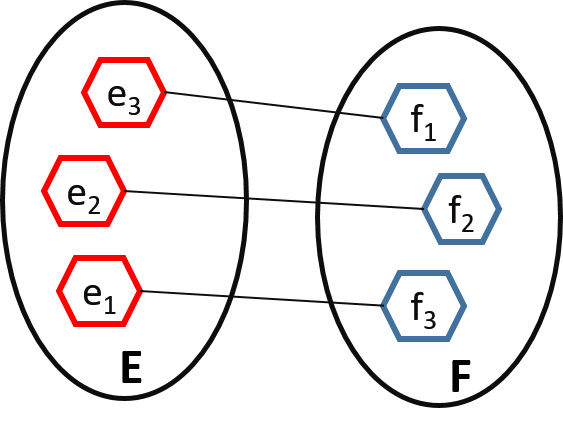
\includegraphics[scale=0.5]{img/ERM-11-11-Relation.png}
\end{figure}
\end{frame}

\begin{frame}{\insertsection}
\framesubtitle{Kardinalitäten auf Entit\"atsmengen und Relationen}
\structure{[n,m]-Beziehung}
\newline 
(E) n: Ordnet einer gegebenen Entit\"at $f_j \in F$ eine oder mehrere Entit\"aten in $E$ zu. 
\newline 
(F) m: Ordnet einer gegebenen Entit\"at $e_i \in E$ eine oder mehrere Entit\"aten in $F$ zu. 
\begin{figure}
	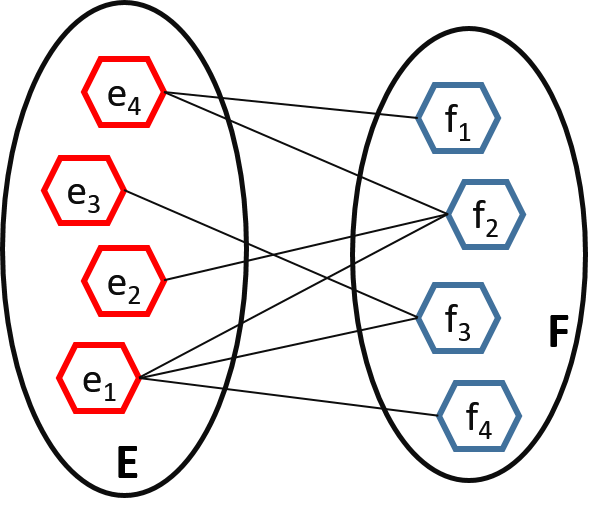
\includegraphics[scale=0.5]{img/ERM-1n-1m-Relation.png}
\end{figure}
\end{frame}

\begin{frame}{\insertsection}
\framesubtitle{Kardinalitäten auf Entit\"atsmengen und Relationen}
\structure{[0..1:0..1]-Beziehung}
  \newline 
  (E) 0..1: Ordnet einer gegebenen Entit\"at $f_j \in F$ keine oder eine Entit\"at in $E$ zu. 
\newline 
  (F) 0..1: Ordnet einer gegebenen Entit\"at $e_i \in E$ keine oder eine Entit\"at in $F$ zu. 
 \begin{figure}
	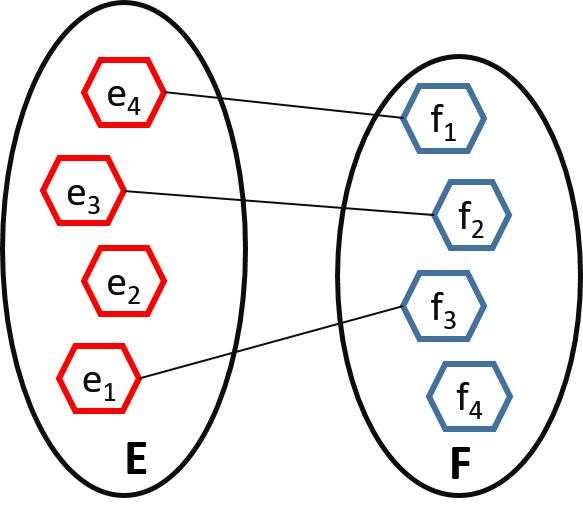
\includegraphics[scale=0.5]{img/ERM-1-1-Relation.png}
 \end{figure}
\end{frame}

\begin{frame}{\insertsection}
\framesubtitle{Kardinalitäten auf Entit\"atsmengen und Relationen}
\structure{[0..1:0..n]-Beziehung}
\newline 
(E) 0..1: Ordnet einer gegebenen Entit\"at $f_j \in F$ keine oder eine Entit\"at in $e_i\in E$ zu. 
\newline 
(F) 0..n: Ordnet einer gegebenen Entit\"at $e_i \in E$ keine, eine oder mehrere Entit\"aten in $F$ zu. 
\begin{figure}
	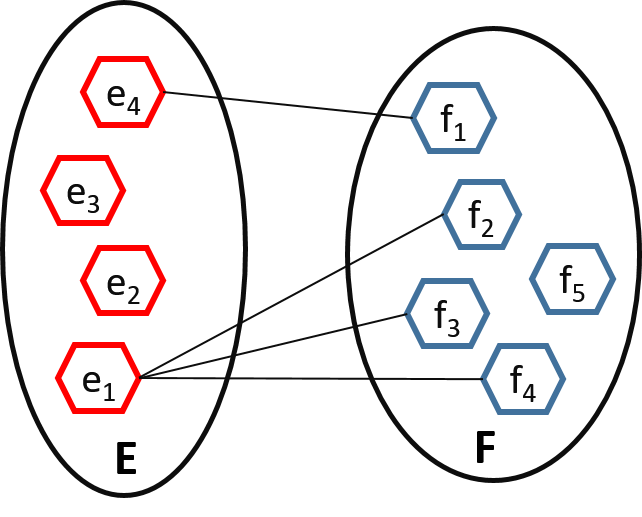
\includegraphics[scale=0.5]{img/ERM-1-n-Relation.png}
\end{figure}
\end{frame}

\begin{frame}{\insertsection}
\framesubtitle{Kardinalitäten auf Entit\"atsmengen und Relationen}
\structure{[0..n:0..m]-Beziehung}
\newline 
(E) 0..n: Ordnet einer gegebenen Entit\"at $f_j \in F$ keine, eine oder mehrere Entit\"aten in $E$ zu. 
\newline 
(F) 0..m: Ordnet einer gegebenen Entit\"at $e_i \in E$ keine, eine oder mehrere Entit\"aten in $F$ zu. 
\begin{figure}
	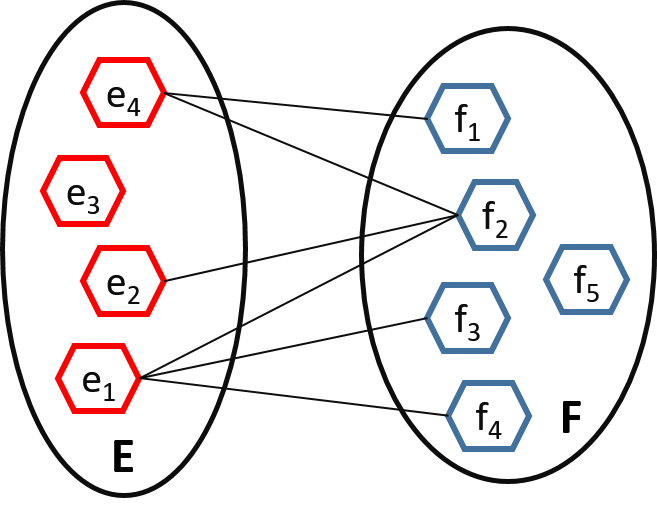
\includegraphics[scale=0.5]{img/ERM-n-m-Relation.png}
\end{figure}
\end{frame}

\begin{frame}{\insertsection}
\framesubtitle{Kardinalitäten auf Entit\"atsmengen und Relationen}
\structure{[n,0..m]-Beziehung}
\newline 
(E) n: Ordnet einer gegebenen Entit\"at $f_j \in F$ eine oder mehrere Entit\"aten in $E$ zu. 
\newline 
(F) 0..m: Ordnet einer gegebenen Entit\"at $e_i \in E$ keine, eine oder mehrere Entit\"aten in $F$ zu. 
\begin{figure}
	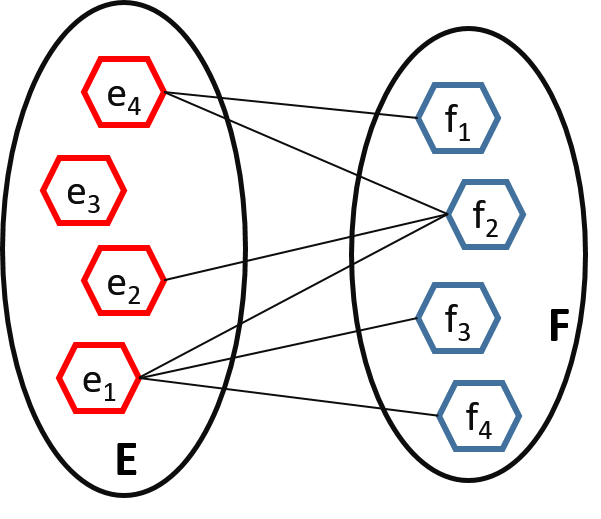
\includegraphics[scale=0.5]{img/ERM-1n-m-Relation.png}
\end{figure}
\end{frame}

\begin{frame}[t]{\insertsection}
\framesubtitle{Kardinalitäten -- tern\"are Beziehungen}
Beziehungen vom Grad $n>2$ benötigen eine besondere Beachtung! 
\abs
\structure{Beispiel:}
\begin{figure}	
	\begin{tikzpicture}[node distance=2em,scale=0.8, transform shape]
	\node[entity] (Professor) {\small Professor}; 
	\node[attribute] (pnr) [below left=of Professor] {\small{\key{PNr}}} edge (Professor);
	\node[relationship] (liest) [right=of Professor] {\small{betreut}} edge node[auto,swap] {1}  (Professor); 
	\node[entity] (Vorlesung) [right=of liest]  {\small{Student}} edge node[auto,swap] {n}  (liest);
	\node[attribute] (vnr) [below right=of Vorlesung] {\small{\key{SNR}}} edge (Vorlesung);
	\node[entity] (Raum) [below=of liest] {\small{Thema}} edge node[auto,swap] {1} (liest); 
	\node[attribute] (datum) [below right=of liest] {\small{{Note}}} edge (liest);
	\node[attribute] (rnr) [left=of Raum] {\small{\key{TNr}}} edge (Raum);
	\end{tikzpicture}	
	\caption{\label{er:ternary}ER-Diagramm mit tern\"arem Beziehungstyp}
\end{figure}		
\alert{\"Ubung: Welche Semantik hat dieses tern\"are Modell?}
\end{frame}

\begin{frame}{\insertsection}
\framesubtitle{Kardinalitäten -- $n$-\"are Beziehungen}
\begin{figure}
	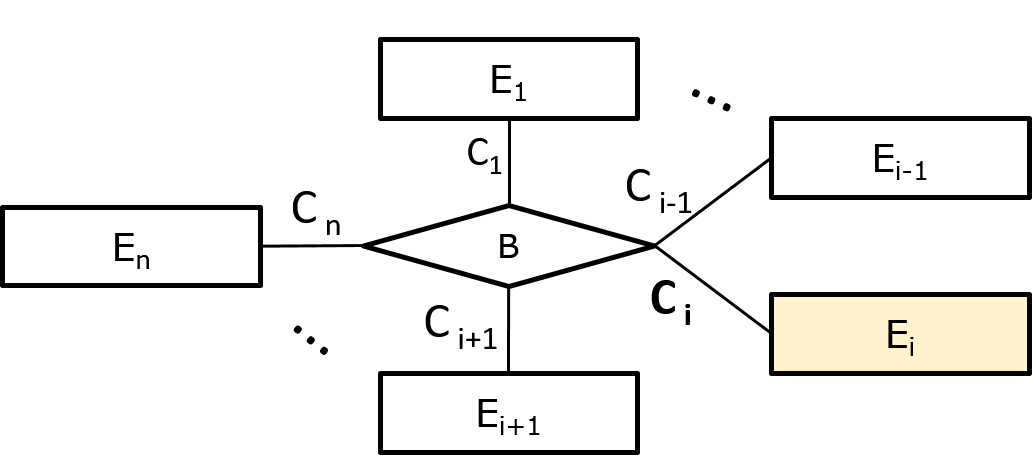
\includegraphics[scale=0.5]{img/ERM-Kardinalitaet.png}
\end{figure}  
\alert{\"Ubung: Machen Sie sich dieses allgemeine Diagramm anhand weiterer Beispiele klar.}
\end{frame}

\begin{frame}{\insertsection}
\framesubtitle{Totale Partizipation}
\begin{definition}[Totale Partizipation] Sei $B$ eine Beziehung zwischen den Entit\"atstypen $E_1, E_2,\ldots, E_n$. 
	Eine totale Partizipation des Entit\"atstyps $E_i$ in der Beziehung $B$ liegt vor, wenn es für \textbf{jede Entit\"at} $\mathbf{e_i}$
	vom Typ $E_i$ mindestens ein Tupel $(e_1,e_2,\ldots,\mathbf{e_i},\ldots,e_n)$ in der Relation $\mathcal{R}(B)$ gibt.
\end{definition} 
\abs
Totale Partizipation dr\"uckt also die zwingende Teilnahme aller Entit\"aten des Entitätstyps $E_i$ an der Beziehung aus. 
\end{frame}

\begin{frame}{\insertsection}
\framesubtitle{Totale Partizipation -- Graphische Notation}
\begin{figure}
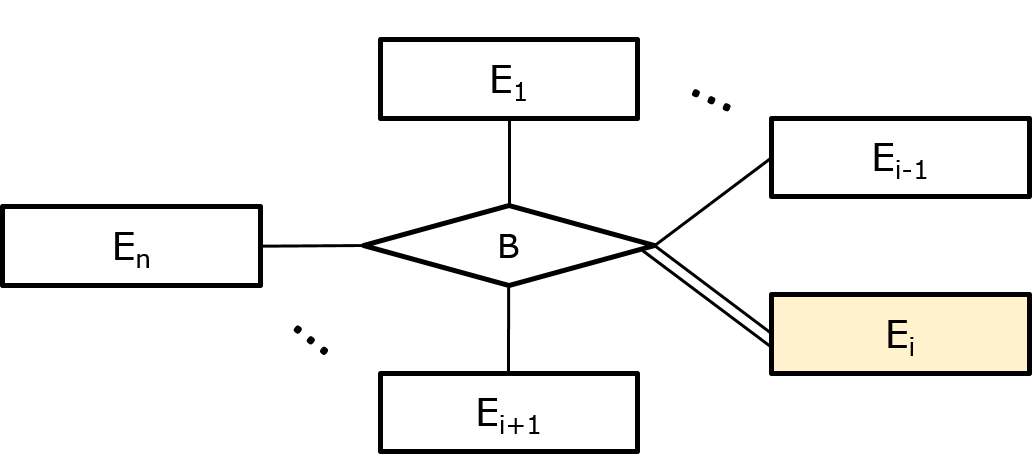
\includegraphics[scale=0.6]{img/ERM-TotalePartizipation.png}
\end{figure}  
\end{frame}

\begin{frame}{\insertsection}
\framesubtitle{Totale Partizipation -- Beispiel}
Abbildung \ref{er:total} dr\"uckt die totale Partizipation des Entit\"atstyps Professor an der Beziehung \emph{leitet} aus. 
Sie setzt also zwingend voraus, dass ein Professor auch (mindestens) einen Studiengang leitet.  
\begin{figure}
\begin{tikzpicture}[node distance=2em]
\node[entity] (Professor) {\small Studiengang}; 
\node[relationship] (leitet) [right=of Professor] {\small{leitet}} edge node[auto,swap] {} (Professor); 
\node[entity] (klausur) [right=of leitet]  {\small{Professor}} edge[total] node[auto,swap] {} (leitet);
\end{tikzpicture}
\caption{\label{er:total}ER-Diagramm mit totaler Partizipation}
\end{figure}		
\end{frame}

%@@@

\begin{frame}[label=isarelation]{\insertsection}
\framesubtitle{Spezielle Beziehungen}
\structure{Für die Abbildung von Generalisierungen / Vererbungen oder Aggregationen können spezielle Beziehungstypen eingesetzt werden.}

\begin{description}[leftmargin=0cm]
\item[is-a] Diese Beziehung verkörpert eine Generalisierung (z.B. Auto is-a Fahrzeug). Sie werden durch 
ein Dreieck dargestellt und verdienen besondere Beachtung bei der Überführung in ein Relationenschema (später in der Vorlesung).
\item[part-of] Diese Beziehung verkörpert eine Aggregation und wird mit einem normalen Beziehungssymbol versehen.
\end{description}

\begin{figure}
% 		\begin{tikzpicture}[node distance=2em]
% 			\node[entity] (Auto) {\small Auto}; 
% 			\node[isa] (ist) [right=of Auto] {\small{is a}} edge (Auto); 
% 			\node[entity] (fahrzeug) [right=of ist]  {\small{Fahrzeug}} edge  (ist);
% 			\node[relationship] (partof) x
% 		\end{tikzpicture}
% 		\caption{ER-Diagramm mit is-a Beziehung}
%	\end{figure}		
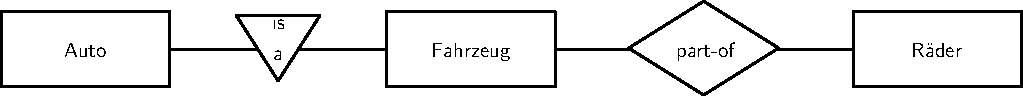
\includegraphics[scale=0.8]{img/genagg.pdf}
\caption{ER-Diagramm mit is-a Beziehung}
\end{figure}
\end{frame}

%\subsection{Schwache Entitäten}
\begin{frame}<1-2>[label=weakentity]
\frametitle<1-2>{\insertsection\framesubtitle{Schwache Entit\"aten}}
\frametitle<3>{\insertsection\framesubtitle{Schwache Entit\"aten -- Wiederholung Folie \ref{weakentity}}}
\onslide
{\structure{\textbf{Schwache Beziehungen}\\[4pt]}}
Beispiel: \emph{Raum} schwacher Entit\"atstyp, kann ohne \emph{Geb\"aude} nicht identifiziert werden.
\begin{figure}\scalebox{0.8}{
		\begin{tikzpicture}[node distance=2em]
		\node[entity] (geb) {\small Geb\"aude}; 
		\node[attribute] (gnr) [above left=2em of geb] {\key{\small GNR}} edge (geb); 
		\node[attribute] (ort) [above=2em of geb] {\small Name} edge (geb);
		\node[ident relationship] (besitzt) [right=of geb] {\small{besitzt}} edge node[auto,swap] {1} (geb); 
		\node[weak entity] (raum) [right=of besitzt]  {\small{Raum}} edge [total] node[auto,swap] {n} (besitzt); 
		\node[attribute] (rnr) [above=of raum] {\small{RNR}} edge (raum);
		\node[attribute] (profname) [above right=of raum] {\small{Groesse}} edge (raum);
		\end{tikzpicture}
	}
	\caption{\label{er:weak}Schwache Entität}
\end{figure}		
\pause[2]
\vspace{-1em}
\begin{itemize}
	\item Schwache Entit\"aten h\"angen in ihrer Existenz von Eigentümerentität ab.
	\item Identifikation schwacher Entitäten nur im Kontext der Eigent\"umerentit\"at.
	\item Eigent\"umerentit\"at kann keine, eine oder mehrere schwache Entit\"aten besitzen.
	\item Schwache Entit\"aten haben keine Attribute, die Schl\"ussel bilden k\"onnen.
\end{itemize}
\end{frame}

\begin{frame}[t]\frametitle{ER-Modellierung}
\framesubtitle{Entwurfsfragen}
\begin{itemize}
\item In ER-Diagrammen liegt der Fokus auf der Darstellung des Schemas, nicht der Instanzen
\item Die Namen von Entitätstypen, Beziehungstypen usw. sollten nach Möglichkeit die Semantik ausdrücken
\item Entitätstypen werden mit Substantiven im Singular benannt
\item ER-Diagramme werden meist stufenweise verfeinert: 
\begin{itemize}
\item Erstes Konzept mit grundlegenden Entitätstypen und Attributen
\item Einfügen von Beziehungstypen und Kardinalitäten
\item Attribute, die in mehreren Entitätstypen vorkommen, können auf einen eigenen Entitätstyp verfeinert werden
\item Zusammenlegung von Entitätstypen (z.B. Entitätstypen mit nur einem Attribut)
\end{itemize}
\end{itemize}
\end{frame}

\begin{frame}[t]\frametitle{ER-Modellierung}
\framesubtitle{Notationen}
\structure{Es existieren viele unterschiedliche Notationsformen von ER-Modellen:}
\begin{itemize}
\item Chen-Notation (nach Peter Chen, 1976)
\item UML-Notation
\begin{itemize}
\item Aussehen ähnlich wie Klassendiagramme 
\item Vererbung etc. möglich
\item Keine Beziehungen vom Grad $n>2$ erlaubt
\end{itemize}
\item Crow's Feet Notation 
\begin{itemize}
\item Ähnlich wie UML-Notation
\item Stellt Kardinalitäten durch Krähenfüsse dar
\end{itemize}
\end{itemize}
\abs
\structure{In der Vorlesung wird die (erweiterte) Chen-Notation weiter verwendet.}
\end{frame}

\section*{Übungsaufgaben}
\begin{frame}[t]
\frametitle{\insertsection}
\begin{alertblock}{Anwendungsfall: ToDo-Liste}
Modellieren Sie das Datenmodell für eine mehrbenutzerfähige ToDo-Liste (Anmerkung: Die Benutzer sollen \textit{nicht} gemeinsam an Projekten arbeiten!). 

\begin{itemize}
\label{todolist}
\item Zu den verschiedenen Benutzern werden Vorname, Nachname, Login und Passwort gespeichert 
\item Jeder Benutzer kann Projekte anlegen, bestehend aus einem Projektnamen 
\item Jedem Projekt können Aufgaben zugeordnet werden. Die Aufgaben werden pro Projekt beginnend mit der Aufgabennummer 1 angelegt und besitzen neben der Aufgabennummer einen Titel und einen Fertigstellungsgrad (in Prozent)
\end{itemize}
\end{alertblock}
\end{frame}

\section*{Übungsaufgaben}
\begin{frame}[t]
\frametitle{\insertsection}
\begin{alertblock}{Anwendungsfall: Flugbuchungssystem}
Eine Airline möchte ein Flugbuchungssystem erstellen. Sie erhalten die folgenden Informationen: 
\begin{itemize}
\item Jedem Flug mit einer Flugnummer wird eine konkrete Maschine mit entsprechenden Abflug- und Ankunftszeiten hinterlegt 
\item Jeder Flug startet und endet an einem Zielflughafen
\item Jeder Flug wird mit einer Maschine geflogen 
\item Eine Maschine wird von einem bestimmten Hersteller gebaut, besitzt eine Bezeichnung und hat eine Kapazität von $n$ Sitzplätzen
\item Zu jedem Passagier werden Name, Vorname, Geburtsdatum und Ausweisnummer gespeichert
\end{itemize}
Modellieren Sie den vorgegebenen Ausschnitt aus der realen Welt mittels eines ER-Diagramms.
\end{alertblock}
\end{frame}

\section{Relationales Datenmodell}

\begin{frame}<1>[label=codd]{\insertsection}
	%\framesubtitle{\insertsubsection}
	\begin{columns}
		\begin{column}{.68\textwidth}
			\begin{block}{Dr. Frank Edgar Codd (1923-2003)}
				\begin{itemize}
					\item Arbeitete bei IBM Research im IBM Almaden Research Center, St. Jose.
					\item Entwickelte das relationale Datenmodell im Jahre 1970: \emph{A relational Model for large shared data banks}
					\item ACM Turing Award im Jahre 1981 für \emph{\glqq fundamental and continuing contributions to the theory 
						and practice of database systems\grqq}
				\end{itemize}
			\end{block}

		\end{column}
		\begin{column}{.30\textwidth}
		 	\begin{figure}
				\pgfuseimage{codd}
			\end{figure}
		\end{column}
	\end{columns}
\end{frame}

\begin{frame}<1>[label=tabledef]{\insertsection}
	\framesubtitle{Motivation}
	Grob gesagt, organisiert das relationale Datenmodell Daten in Form von Tabellen und Beziehungen zwischen Tabellen.\abs
	\begin{columns}
		\begin{column}{.40\textwidth}
			Eine Tabelle besteht aus
			\begin{itemize}
				\item eindeutigem Namen
				\item Attributen (Spalten) über Wertebereichen (Domänen) 
				\item Tupeln oder \emph{Datens\"atzen} (Zeilen)
			\end{itemize}
		\end{column}
		\begin{column}{.56\textwidth}
			\begin{tabular}{|c|c|c|c|c|}\hline
				\multicolumn{5}{|c|}{\small \textbf{Kunde}}\\\hline\hline
				 \small \textbf{KNR} & \small \textbf{Vorname} & \small \textbf{Name} & \small \textbf{PLZ} & \small \textbf{Ort} \\\hline
				\small 1 &\small Elsa &\small Musterfrau &\small 68165 &\small Mannheim \\\hline
				\small 2 & \small Max &\small  Mustermann & \small 57234 &\small Wilnsdorf \\\hline
				$\cdots$ & $\cdots$ & $\cdots$ & $\cdots$ & $\cdots$ \\\hline
			\end{tabular}
		\end{column}
	\end{columns}
\end{frame}

\subsection{Formale Definition}

\begin{frame}
\frametitle{\insertsection}
\framesubtitle{\insertsubsection \ -- Datenbankschema}
\onslide
\begin{itemize}
	\item In logischen Datenmodellen werden Daten durch \emph{Datenbankschemata} beschrieben.
	\pause
	\item Ein Datenbankschema berücksichtigt dabei folgende Aspekte der Daten:
	\begin{itemize} 
		\item Struktur und Datentypen
		\item Zul\"assige Wertebereiche 
		\item Beziehungen
		\item Abh\"angigkeiten
		\item Identifizierbarkeit und Eindeutigkeit
	\end{itemize}
	\pause
	\item Durch ein Datenbankschema werden somit Bedingungen an die Daten definiert. 
	\begin{itemize}
		\item Diese Bedingungen nennt man \emph{Integrit\"atsbedingungen}.
		\item Integrit\"atsbedingungen k\"onnen syntaktischer oder (meistens) semantischer Natur sein.
		\item Die \"Uberpr\"ufung der Integrit\"atsbedingungen erfolgt durch das Datenbanksystem.
	\end{itemize}
	\pause
	\item Im relationalen Modell werden Tabellen durch ein \emph{Relationenschema} definiert.
	\begin{itemize}
		\item Ein Relationenschema ist Teil des Datenbankschemas.
	\end{itemize}	
\end{itemize}
\end{frame}

\begin{frame}
\frametitle{\insertsection}
\framesubtitle{\insertsubsection}
\begin{block}{\textbf{Vorab: Wiederholung des Begriffs \emph{Relation}}}
Seien $M_1$, $M_2$, $\ldots$, $M_n$ Mengen. Eine $n$-stellige Relation $R$ ist eine Teilmenge des $n$-fachen 
kartesischen Produktes $M_1 \times M_2 \times \cdots \times M_n$.
\begin{equation*} 
R \subseteq M_1 \times M_2 \times \cdots \times M_n
\end{equation*} 
\structure{Eine konkrete Relation ist daher eine (ungeordnete) Menge von geordneten $n$-Tupeln:}
\begin{equation*} 
R = \{(x_{11}, x_{12},\dots,x_{1n}),(x_{21}, x_{22},\dots,x_{2n}),\dots,(x_{k1}, x_{k2},\dots,x_{kn})\}
\end{equation*} 
\end{block}
\end{frame}

\begin{frame}
 \frametitle{\insertsection}
 \framesubtitle{\insertsubsection}
 \structure{Tabellenartige Darstellung der Relation $R$:}
 \begin{table}
  \begin{tabular}{cccc}\\\toprule
   \textbf{$M_1$} &\textbf{$M_2$}& \textbf{$\dots$} & \textbf{$M_n$}\\\midrule
   $x_{11}$ & $x_{12}$ & $\dots$ & $x_{1n}$ \\
   $x_{21}$ & $x_{22}$ & $\dots$ & $x_{2n}$ \\
   $\dots$ & $\dots$ & $\dots$ & $\dots$ \\
   $x_{k1}$ & $x_{k2}$ & $\dots$ & $x_{kn}$ \\\bottomrule
  \end{tabular}
 \end{table}
 \end{frame}

\begin{frame}\frametitle{\insertsection}
	\framesubtitle{\insertsubsection}
	\begin{definition}[Dom\"ane]\label{def:domain}
		Eine Dom\"ane $D$ ist die Menge der erlaubten Werte eines Datentyps in einem bestimmten Kontext. Eine Dom\"ane
		hei\ss t \emph{atomar}, wenn ihre Werte nicht weiter teilbar sind.
	\end{definition}
\abs
	Beispiele für Dom\"anen:
	\begin{itemize}
		\item Die Menge der natürlichen Zahlen $\mathbb{N}$
		\item RGB-Farbenskala
		\item Postleitzahlen
		\item Geburtsdaten
	\end{itemize}
\abs
\end{frame}

\begin{frame}\frametitle{\insertsection}
\framesubtitle{\insertsubsection}
\begin{definition}[Attribute]\label{def:att}
	Ein Attribut $A$ ist eine Rollenbezeichnung oder die Variable einer Dom\"ane $D$. 
	Die Dom\"ane eines Attributs $A$ wird mit $\text{dom}(A)$ bezeichnet.
\end{definition}
\abs
\structure{Ein \emph{zul\"assiger Attributwert} f\"ur ein Attribut $A$ ist ein Wert aus der Dom\"ane $D=\text{dom}(A)$.}
\abs\abs 
Beispiele für Attribute:
\begin{itemize}
	\item $RGB$ mit $\text{dom}(RGB) =$ RGB-Farbenskala
	\item $PLZ$ mit $\text{dom}(PLZ) =$ Postleitzahlen
	\item $Date\_of\_Birth$ mit $\text{dom}(Date\_of\_Birth) =$ Geburtsdaten
\end{itemize}
\end{frame}

\begin{frame}\frametitle{\insertsection}
\framesubtitle{\insertsubsection}
\begin{definition}[Relationenschema]\label{def:schema}
	Ein $n$-stelliges oder $n$-\"ares Relationenschema $\mcl{R}(N\mid A_1:D_1,A_2:D_2,\ldots,A_n:D_n)$ besteht aus einem Namen 
	$N$, Attributen $A_1, A_2,\ldots, A_n$ und deren zugehöriger Domänen $D_1, D_2, \ldots, D_n$ (und weiterer Metadaten -- 
	sp\"ater dazu mehr). 
\end{definition}
\pause
\textbf{Beachte:} Der Name $N$ des Schemas wird im Folgenden oft implizit angegeben oder weggelassen, wenn er aus dem 
Zusammenhang klar oder nicht relevant ist.\\[5pt]
\onslide \pause
\textbf{Beispiel eines Relationenschemas:}\\
\texttt{$\mcl{R}$(Kunde$\mid$KNR:int,Vorname:string,Name:string,PLZ:string,Ort:string)}\\[5pt]
\textbf{Schreibweise ohne Name:}\\
\texttt{$\mcl{R}$(KNR:int,Vorname:string,Name:string,PLZ:string,Ort:string)}\\[5pt]
\textbf{Schreibweise mit implizitem Namen und ohne Angabe der Domänen:}\\
\texttt{Kunde(KNR, Vorname, Name, PLZ, Ort)}
\end{frame}

\begin{frame}\frametitle{\insertsection}
\framesubtitle{\insertsubsection}
\begin{definition}{Relation eines Relationenschemas}\label{def:rel}
	Sei $\mcl{R}(A_1:D_1,A_2:D_2,\ldots,A_n:D_n)$ ein Relationenschema. 
	Eine \emph{Relation des Relationenschemas} $\mcl{R}$ ist eine Relation  
  $R\subseteq D_1\times\ldots D_n$. Bezeichnung: $R\langle\mcl{R}\rangle$.
\end{definition}
\onslide\pause
\abs
Konkret ist eine Relation $R$ des Relationenschemas $\mcl{R}(A_1,A_2,\dots,A_n)$ eine Menge von 
$n$-Tupeln der Form $t=(v_1,v_2,\ldots,v_n)$ mit $v_i \in D_i$ f\"ur alle $i=1,\ldots,n$.
\end{frame}

\begin{frame}\frametitle{\insertsection}
\framesubtitle{\insertsubsection}
\textbf{Beispiel}\\
\abs
Relationenschema: \texttt{Kunde(KNR, Vorname, Name, PLZ, Ort)}
\abs
Eine Relation $R$ des Schemas \texttt{Kunde} (tabellenartige Darstellung):
\begin{center}
	\begin{tabular}{|c|c|c|c|c|}\hline
		\multicolumn{5}{|c|}{\small \textbf{Kunde}}\\\hline\hline
		\small \textbf{KNR} & \small \textbf{Vorname} & \small \textbf{Name} & \small \textbf{PLZ} & \small \textbf{Ort} \\\hline
		\small 1 &\small Elsa &\small Musterfrau &\small 68165 &\small Mannheim \\\hline
		\small 2 & \small Max &\small  Mustermann & \small 57234 &\small Wilnsdorf \\\hline
		$\cdots$ & $\cdots$ & $\cdots$ & $\cdots$ & $\cdots$ \\\hline
	\end{tabular}
\end{center}
\end{frame}

\begin{frame}\frametitle{\insertsection}
\framesubtitle{\insertsubsection}
In einer Relation kann es keine zwei gleiche Tupel geben. Warum?
\onslide\pause
\begin{center}
	\begin{tabular}{|c|c|c|c|}\hline
		\multicolumn{4}{|c|}{\small \textbf{Kunde}}\\\hline\hline
		\small \textbf{Vorname} & \small \textbf{Nachname} & \small \textbf{PLZ} & \small \textbf{Ort} \\\hline
		\rowcolor{Red}
		\small Elsa &\small Musterfrau &\small 68165 &\small Mannheim \\\hline
		\small Max &\small  Mustermann & \small 57234 &\small Wilnsdorf \\\hline
		$\cdots$ & $\cdots$ & $\cdots$ & $\cdots$ \\\hline
		\rowcolor{Red}
		\small Elsa &\small Musterfrau &\small 68165 &\small Mannheim \\\hline
	\end{tabular}
\end{center}
\abs 
\alert{Eine Relation ist eine Menge. Somit darf es die rot markierten Tupel allenfalls einmal geben!}
\end{frame}

\subsection{Funktionale Abhängigkeiten}

\begin{frame}\frametitle{\insertsection}
\framesubtitle{\insertsubsection}
\begin{definition}[Projektion]
	Sei $\mcl{R}(A_1,A_2,\ldots,A_n)$ ein Relationenschema und $X$ eine Teilmenge der Attribute, d.~h.~$X\subseteq\{A_1,\ldots,A_n\}$.
	Sei $R$ eine Relation des Schemas $\mcl{R}$ und $t\in R$ ein Tupel dieser Relation. Dann ist $\Pi_X(t)$ die Projektion des Tupels 
	$t$ auf die Komponenten aus $X$.
\end{definition}
\end{frame}

\begin{frame}\frametitle{\insertsection}
\framesubtitle{\insertsubsection}
\textbf{Beispiel einer Projektion}
\abs
Relationenschema \texttt{Kunde(KNR, Vorname, Name, PLZ, Ort)}
\nl 
Attributmenge $X=\{$\texttt{KNR, Name}$\}$
\nl
Eine Relation $R$ von Schema \texttt{Kunde}:
\begin{center}
	\begin{tabular}{|c|c|c|c|c|}\hline
		\multicolumn{5}{|c|}{\small \textbf{Kunde}}\\\hline\hline
		\small \textbf{KNR} & \small \textbf{Vorname} & \small \textbf{Name} & \small \textbf{PLZ} & \small \textbf{Ort} \\\hline
		\small 1 &\small Elsa &\small Musterfrau &\small 68165 &\small Mannheim \\\hline
		\small 2 & \small Max &\small  Mustermann & \small 57234 &\small Wilnsdorf \\\hline
		$\cdots$ & $\cdots$ & $\cdots$ & $\cdots$ & $\cdots$ \\\hline
	\end{tabular}
\end{center}
\onslide\pause
\nl
Ein Tupel $t =($1, Elsa, Musterfrau, 68165, Mannheim$)$ in Relation $R$
\pause
\abs
Projektion $\Pi_X(t)=($1, Musterfrau$)$
\end{frame}

\begin{frame}[t]\frametitle{\insertsection}
\framesubtitle{\insertsubsection}
\begin{definition}[Funktionale Abhängigkeit]
	\label{def:functionalDependencie}
	Sei $\mcl{R}(A_1,A_2,\ldots,A_n)$ ein Relationenschema und $X, Y\subseteq \{A_1,\ldots,A_n\}$.
	\nl 
	Auf dem Schema $\mcl{R}$ besteht eine \emph{funktionale Abh\"angigkeit} von $X$ nach $Y$, wenn in einer beliebigen 
	Relation $R$ von $\mcl{R}$ alle Tupel $s,t\in R$ der Bedingung
	\begin{equation*}
	\Pi_X(s) = \Pi_X(t) \Rightarrow \Pi_Y(s) = \Pi_Y(t)
	\end{equation*}
	zu gehorchen haben. Bezeichnung: $X\rightarrow Y$
	\abs
	$X$ wird die \emph{Determinante} von $Y$ genannt.
\end{definition}
\onslide\pause 
\begin{itemize}
	\item Funktionale Abhängigkeiten sind semantischer Natur.
	\item Funktionale Abhängigkeiten sind eine spezielle Form von Integrit\"atsbedingungen.
	\item Analogie: Eine Funktion erzeugt für gleiche Eingabewerte stets gleiche Ausgabewerte.
\end{itemize}
\end{frame}

\begin{frame}[t]\frametitle{\insertsection}
\framesubtitle{\insertsubsection}
\begin{block}{\textbf{Folge aus Definition \ref{def:functionalDependencie}}}
	\abs
	Es gelte auf dem Relationenschema $\mcl{R}(A_1,A_2,\ldots,A_n)$ die funktionale Abhängigkeit $X\rightarrow Y$ für  
	$X, Y\subseteq \{A_{1},\ldots,A_{n}\}$. Seien $s$ und $t$ 
	Tupel in einer Relation $R\langle\mcl{R}\rangle$ des Schemas $\mcl{R}$. Wenn $s(A)=t(A)$ f\"ur alle 
	$A\in X$ gilt, dann folgt daraus $s(A^\prime)=t(A^\prime)$ f\"ur alle $A^\prime\in Y$
\end{block}
\end{frame}

\begin{frame}[t]\frametitle{\insertsection}
	\framesubtitle{\insertsubsection}
	\structure{Beispiel: Eine Person besitzt (ggf. mehrere) Autos}
	\begin{center}
		\begin{tabular}{|c|c|c|c|c|c|}\hline
			\multicolumn{6}{|c|}{\small \textbf{Person\_Auto}}\\\hline\hline
			\small \textbf{PNr} & \small \textbf{Vorname}&\small \textbf{Nachname}&\small\textbf{Kennzeichen} &\small\textbf{Typ} & \small\textbf{Baujahr} \\\hline
			\small 1 &\small Max & \small Mustermann &\small MA-BC 111 &\small VW &\small 2013 \\\hline
			\small 1 &\small Max & \small Mustermann &\small MA-BC 112 &\small Audi &\small 2011 \\\hline
			\small 3 &\small Erika &\small Musterfrau &\small LU-BY 42 &\small  Ford &\small 2014 \\\hline
			\small 3 &\small Erika &\small Musterfrau &\small LU-EM 4711 &\small  Smart &\small 2012 \\\hline
		\end{tabular}
	\end{center}
	\structure{Funktionale Abhängigkeiten:}
	\begin{equation*}
	\begin{split}
   \{PNr, Kennzeichen\}&\rightarrow\{Vorname, Nachname, Typ, Baujahr\}\\
   \{PNr\}&\rightarrow\{Vorname, Nachname\}\\
   \{Kennzeichen\}&\rightarrow\{Typ, Baujahr\}
  \end{split}
	\end{equation*}
\end{frame}

\begin{frame}[t]\frametitle{\insertsection}
\framesubtitle{\insertsubsection}\label{frame:inferenzregeln}
\begin{theorem}[Inferenzregeln]
	%\structure{\textbf{Inferenzregeln}}
	%\abs
	Gegeben seien Attributmengen $X,Y,Z,V,W \subseteq \{A_1,A_2,\ldots,A_n\}$ eines Relationenschemas $\mcl{R}(A_1,A_2,\ldots,A_n)$. 
	Dann gilt:
	\begin{alignat*}{2}
	\text{[Sub-Reflexivität]}& &\quad Y\subseteq X &\Rightarrow X \rightarrow Y\\
	\text{[Zerlegung]}& &\quad \{X\rightarrow Y\cup Z\}&\Rightarrow\{X\rightarrow Y\}\wedge\{X\rightarrow Z\}\\
	\text{[Vereinigung]}& &\quad \{X\rightarrow Y\}\wedge\{V\rightarrow W\}&\Rightarrow\{X\cup V\rightarrow Y\cup W\}\\
	\text{[Augmentation]}& &\quad \{X\rightarrow Y\}&\Rightarrow\{X\cup Z\rightarrow Y\cup Z\}\\
	\text{[Pseudotransitivität]}& &\quad \{X\rightarrow Y\}\wedge\{Y\cup W\rightarrow Z\}&\Rightarrow\{X\cup W\rightarrow Z\}\\
	\textbf{Folge:}& & &\\
	\text{[Reflexivität]}& &\quad X\rightarrow X &\quad\forall\,X\\
	\text{[Transitivität]} & & \quad \{X\rightarrow Y\}\wedge \{Y\rightarrow Z\}&\Rightarrow\{X\rightarrow Z\}
	\end{alignat*}
\end{theorem}
%\pause
%\alert{Funktionale Abh\"angigkeit ist im i.~a.~nicht kommutativ: $\{X\rightarrow Y\} \nRightarrow \{Y\rightarrow X\}$.}
\end{frame}

\begin{frame}\frametitle{\insertsection}
\framesubtitle{\insertsubsection}
\begin{definition}[Volle funktionale Abhängigkeit]
	Seien $X,Y\subseteq \{A_1,A_2,\ldots,A_n\}$ Attributmengen eines Relationenschemas $\mcl{R}(A_1,A_2,\ldots,A_n)$.\nl
	$Y$ heißt \textit{voll funktional abhängig} von $X$, wenn $X\rightarrow Y$, und f\"ur alle echten Untermengen $X^\prime \subsetneq X$ 
	gilt $X^\prime\nrightarrow Y$. 
	\nl
	Schreibweise: $X{\large\rightrightarrows} Y$
\end{definition}
\onslide\pause 
\begin{itemize}
	\item $X\rightrightarrows Y$ bedeutet also, dass aus der Attributmenge $X$ kein Attribut entfernt werden kann, 
	ohne die funktionale Abhängigkeit zu zerstören. 
	\item Wenn $\vert X\vert = 1$, dann folgt aus $X\rightarrow Y$ stets $X\rightrightarrows Y$.
\end{itemize}
\end{frame}

\begin{frame}[t]\frametitle{\insertsection}
	\framesubtitle{\insertsubsection}
	\structure{Beispiel:}
	\begin{center}
		\begin{tabular}{|c|c|c|c|c|c|}\hline
			\multicolumn{6}{|c|}{\small \textbf{Mitarbeiter\_Projekt}}\\\hline\hline
			\small \textbf{MANr} & \small \textbf{Vorname}&\small \textbf{Nachname}&\small\textbf{PNr} &\small\textbf{Projektname} 
			& \small\textbf{Funktion} \\\hline
			\small 1 &\small Max & \small Mustermann &\small 4712 & \small Test &\small Unit-Tests \\\hline
			\small 1 &\small Max & \small Mustermann &\small 4713 &\small Vertrieb & \small Kampagnen \\\hline
			\small 2 &\small Erika &\small Musterfrau &\small 4712 &\small Test &\small Integrations-Tests \\\hline
		\end{tabular}
	\end{center}
	In diesem Beispiel gilt die funktionale Abhängigkeit $\{MANr, PNr\}\rightarrow\{Vorname, Nachname, Projektname, Funktion\}$.
	\nl 
	Es gilt aber auch:\nl
	$\{PNr\}\rightarrow\{Projektname\}$, somit ist $Projektname$ nicht voll funktional abhängig von $\{MANr, PNr\}$.
\end{frame}

\subsection{Schlüssel}

\begin{frame}\frametitle{\insertsection}
\framesubtitle{\insertsubsection}
Sei $\mcl{R}(A_1,A_2,\ldots,A_n)$ ein Relationenschema.	
\begin{definition}[Superschlüssel]\label{def:superkey}
	Ein Superschlüssel $S \subseteq \{A_1,A_2,\ldots,A_n\}$ von $\mcl{R}$ ist eine Menge von \texttt{non-null}-Attributen, 
	von der die gesamte Attributmenge funktional abh\"angig ist. Das hei\ss t $S\rightarrow \{A_1,A_2,\ldots,A_n\}$.     	
\end{definition}
%
\begin{definition}[Kandidatenschlüssel]\label{def:candkey}
	Ein Schlüsselkandidat $K$ ist ein Superschlüssel, von der die gesamte Attributmenge voll funktional abh\"angig ist. 
	Das hei\ss t $K\rightrightarrows \{A_1,A_2,\ldots,A_n\}$.     	
\end{definition}
%
\begin{definition}[Primärschlüssel]\label{def:primarykey}
	\textit{Genau ein} Schlüsselkandidat wird als Primärschlüssel des Schemas festgelegt.
\end{definition}
\end{frame}

\begin{frame}\frametitle{\insertsection}
\framesubtitle{\insertsubsection}
\onslide
\structure{Mit anderen Worten:}
\begin{itemize}
\item Ein Superschlüssel $S$ ist eine Menge von Attributen, deren Werte die eindeutige Identifizierbarkeit eines Tupels 
garantiert.
\pause
\item Ein Schlüsselkandidat $K$ ist ein minimaler Superschlüssel, d.~h.~die Attributmenge in $K$, die die eindeutige 
Identifizierbarkeit von Tupeln gew\"ahrleistet, kann nicht weiter verkleinert werden.
\pause
\item In manchen Datenbanken werden auch Superschl\"ussel als Prim\"arschl\"ussel zugelassen, die keine Kandidatenschl\"ussel sind. 
Beispiel: PostgreSQL.
\end{itemize} 
\end{frame}

\begin{frame}\frametitle{\insertsection}
 \framesubtitle{\insertsubsection}
 \structure{Beispiel:}
 \nl
 Schema \texttt{Artikel(EAN, LfdNr, Regalnr, Regalfachnr, Name, Stückzahl)}
	\begin{itemize}
		\item Superschlüssel
		\begin{itemize}
			\item {EAN, LfdNr, Regalnr, Regalfachnr, Name}
			\item {EAN, LfdNr, Regalnr, Regalfachnr}
			\item {Regalnr, Regalfachnr}
			\item {EAN}
			\item ...
		\end{itemize}
		\item Kandidatenschlüssel
		\begin{itemize}
			\item EAN
			\item LfdNr
                         \item {Regalnr, Regalfachnr}
		\end{itemize}
		\item{Gewählter Primärschlüssel}
		\begin{itemize}
			\item EAN
		\end{itemize}
	\end{itemize}
\end{frame}

\begin{frame}\frametitle{\insertsection}
	\framesubtitle{\insertsubsection}
		\structure{Beispiel: Relationenschema \textit{Kunde}:}
			\begin{center}
				\begin{tabular}{|c|c|c|c|c|}\hline
				\multicolumn{5}{|c|}{\small \textbf{Kunde}}\\\hline\hline
				 \cellcolor{Green}\small \textbf{\key{KNR}} & \small \textbf{Vorname} & \small \textbf{Nachname} & \small \textbf{PLZ} & \small \textbf{Ort} \\\hline
				\cellcolor{Green}\small 1 &\small Elsa &\small Musterfrau &\small 68165 &\small Mannheim \\\hline
				\cellcolor{Green}\small 2 & \small Max &\small  Mustermann & \small 57234 &\small Wilnsdorf \\\hline
				\cellcolor{Green}$\cdots$ & $\cdots$ & $\cdots$ & $\cdots$ & $\cdots$ \\\hline
			\end{tabular}
			\end{center}
 \begin{itemize}
	\item Attribut \texttt{KNR} identifiziert einen Kunden eindeutig und kann als Prim\"arschl\"ussel dienen.
	\item Sowohl im Relationenschema als auch in der Relation selbst wird der Primärschlüssel unterstrichen dargestellt:\\
		\centerline{\texttt{Kunde(\key{KNR},Vorname,Nachname,PLZ,Ort)}}	
 \end{itemize}
\end{frame}

\begin{frame} 
\frametitle{\insertsection}
\framesubtitle{\insertsubsection \ -- Fremdschl\"ussel (Motivation)}
\begin{columns}
	\begin{column}{.48\textwidth}
		\begin{center}
			\begin{tabular}{|c|c|c|}\hline
				\multicolumn{3}{|c|}{\small \textbf{Kunde}}\\\hline\hline
				\cellcolor{Green}\small \textbf{\key{KNR}} & \small \textbf{Vorname} & \small \textbf{Nachname}  \\\hline
				\cellcolor{Green}\small 1 &\small Elsa &\small Musterfrau \\\hline
				\cellcolor{Green}\small 2 & \small Max &\small  Mustermann  \\\hline
				\cellcolor{Green}\small 3 & \small Hans &\small  Fritsche  \\\hline
				\cellcolor{Green}$\cdots$ & $\cdots$ & $\cdots$  \\\hline
			\end{tabular}
		\end{center}
	\end{column}
	\begin{column}{.48\textwidth}
		\begin{center}
			\begin{tabular}{|c|c|c|}\hline
				\multicolumn{3}{|c|}{\small \textbf{Auftrag}}\\\hline\hline
				\cellcolor{Green}\small \textbf{\key{ANR}} & \cellcolor{Yellow}\small \textbf{KdNr} & \small \textbf{Datum}  \\\hline
				\cellcolor{Green}\small 1001 &\cellcolor{Yellow}\small 1 &\small 02.01.2013 \\\hline
				\cellcolor{Green}\small 1002 &\cellcolor{Yellow}\small 2 &\small  04.05.2013  \\\hline
				\cellcolor{Green}\small 1003 &\cellcolor{Yellow}\small 2 &\small  03.01.2014  \\\hline
				\cellcolor{Green}$\cdots$ & \cellcolor{Yellow}$\cdots$ & $\cdots$  \\\hline
			\end{tabular}
		\end{center}
	\end{column}
\end{columns}
\abs
Attribut \texttt{KdNr} in Relation \texttt{Auftrag} verweist auf Prim\"arschl\"ussel \underline{\texttt{KNR}} 
in Relation \texttt{Kunde}.
\end{frame}

\begin{frame}\frametitle{\insertsection}
\framesubtitle{\insertsubsection}
\onslide
\begin{definition}[Fremdschlüssel] 
Seien $\mcl{R}$ und $\mcl{S}$ Relationenschemata. 
\nl
Sei $P=\{A_1,\ldots, A_p\}$ Prim\"arschl\"ussel von $\mcl{R}$ 
und $F=\{B_1,\ldots B_p\}$ eine Attributmenge von $\mcl{S}$. 
\\[8pt]
Dann hei\ss t $F$ Fremdschl\"ussel in $\mcl{S}$ zum Prim\"arschl\"ussel $P$ in $\mcl{R}$, wenn gilt:
\begin{enumerate}
	\pause
	\item $\text{dom}(A_i) = \text{dom}(B_i)$ f\"ur alle $i\in\{1,\ldots,p\}$
	\pause
	\item\label{map-foreign-key} In einer Relation $S$ von $\mcl{S}$ kann ein Datensatz/Tupel $s$ nur existieren, wenn es in der 
	Relation $R$ von $\mcl{R}$ bereits einen Datensatz $r$ gibt mit $\Pi_P(r)=\Pi_F(s)$.
	\pause
	\item 
	Ein Datensatz $r$ in Relation $R$ kann nur gel\"oscht werden, wenn es keine Datensätze $s$ in $S$ gibt,
	die {gem\"a\ss} (\ref{map-foreign-key}) mit $r$ in Beziehung stehen.
\end{enumerate}
\end{definition}
\end{frame} 

\begin{frame} 
\frametitle{\insertsection}
\framesubtitle{\insertsubsection}
\begin{itemize}
	\onslide
	\item $\mcl{R}$ hei\ss t \emph{referenziertes} Schema (fortan Prim\"arschema) und $\mcl{S}$ \emph{referenzierendes} Schema 
	(fortan Fremdschema).\\[4pt]
	\pause 
	\item Fremdschl\"ussel $=$ Menge von Attributen in Relation $S$ (Fremdschema), deren \texttt{non-null}-Werte 
	(in Tupeln von $S$) garantiert als Prim\"arschl\"ussel in Tupeln in Relation $R$ (Prim\"arschema) vorkommen.\\[4pt]
	\pause 
	\item Fremdschl\"ussel in der Relation des Fremdschemas nicht eindeutig.\\[4pt]
	\pause 
	\item Fremdschema kann Fremdschl\"ussel zu Prim\"arschl\"usseln von einem oder mehreren Prim\"arschemata haben.\\[4pt]
	\pause 
	\item Fremdschl\"usselbeziehungen sind Integrit\"atsbedingungen $\rightarrow$ \emph{referenzielle Integrit\"at}\\[4pt] 
	\pause 
	\item Die Integrit\"atsbedingungen sind f\"ur Tupel des Fremdschemas mit \texttt{null}-Werten im Fremdschl\"ussel 
	au\ss er Kraft gesetzt.
\end{itemize}
\end{frame}

% vvvvvvvvv nicht in die Präsentation aufnehmen vvvvvvvvvv
\nowrite{
\begin{frame} 
\frametitle{\insertsection}
\framesubtitle{\insertsubsection \ -- Beispiel}
\begin{columns}
\begin{column}{.48\textwidth}
\begin{center}
	\begin{tabular}{|c|c|c|}\hline
		\multicolumn{3}{|c|}{\small \textbf{$\mcl{R}$: Kunde}}\\\hline\hline
		\cellcolor{Green}\small \textbf{\key{KNR}} & \small \textbf{Vorname} & \small \textbf{Nachname}  \\\hline
		\cellcolor{Green}\small 1 &\small Elsa &\small Musterfrau \\\hline
		\cellcolor{Green}\small 2 & \small Max &\small  Mustermann  \\\hline
		\cellcolor{Green}\small 3 & \small Hans &\small  Fritsche  \\\hline
		\cellcolor{Green}$\cdots$ & $\cdots$ & $\cdots$  \\\hline
	\end{tabular}
\end{center}
\end{column}
\begin{column}{.48\textwidth}
\begin{center}
	\begin{tabular}{|c|c|c|}\hline
		\multicolumn{3}{|c|}{\small $\mcl{S}$: \textbf{Auftrag}}\\\hline\hline
		\cellcolor{Green}\small \textbf{\key{ANR}} & \cellcolor{Yellow}\small \textbf{KNR} & \small \textbf{Datum}  \\\hline
		\cellcolor{Green}\small 1001 &\cellcolor{Yellow}\small 1 &\small 02.01.2013 \\\hline
		\cellcolor{Green}\small 1002 &\cellcolor{Yellow}\small 2 &\small  04.05.2013  \\\hline
		\cellcolor{Green}\small 1003 &\cellcolor{Yellow}\small 2 &\small  03.01.2014  \\\hline
		\cellcolor{Green}$\cdots$ & \cellcolor{Yellow}$\cdots$ & $\cdots$  \\\hline
	\end{tabular}
\end{center}
\end{column}
\end{columns}
\end{frame}
}
% ^^^^^^^^^^ nicht in Präsentation aufnehmen ^^^^^^^^^^

\begin{frame}\frametitle{\insertsection}
	\framesubtitle{\insertsubsection}
	\structure{Business Key/Natural Key versus Technical Key/Surrogate Key}\\[8pt]
	\begin{itemize}
		\item Business Key/Natural Key
		\begin{itemize}
			\item Schlüssel, der in natürlicher Weise einer Entität zugeordnet werden kann 
			\item Beispiele: Kundennummern, Fahrgestellnummern, Seriennummern\\[8pt]
		\end{itemize}
		\item Technical Key/Surrogate Key
		\begin{itemize}
			\item Existiert kein natürlicher Schlüssel, muss ein künstliches Schlüsselattribut eingefügt werden.
			\item Beispiel: Laufende Nummer eines Eingangssignals bei Zeitreihen
		\end{itemize}
	\end{itemize}
\end{frame}

\begin{frame}\frametitle{\insertsection}
\framesubtitle{\insertsubsection}
\onslide
\begin{definition}[Eindeutige Attribute / Unique Attributes]\label{unique-attr}
	Sei $\mcl{R}(A_1,\ldots, A_n)$ ein Relationenschema und $X\subseteq \{A_1,\ldots, A_n\}$ eine ausgew\"ahlte 
	Menge von Attributen von $\mcl{R}$. Dann nennt $X$ eindeutig (unique), wenn f\"ur jedes 
	Tupel $t$ in einer Relation $R$ von $\mcl{R}$ die Projektion $\Pi_X(t)$ in $\Pi_X(R)$ nur genau einmal 
	vorkommen darf.
\end{definition}
\pause
\abs
\begin{itemize}
	\item Eindeutigkeit ist eine (semantische) Integrit\"atsbedingung.
	\item Es kann \texttt{null}-Attribute in $X$ geben.
	\item Nicht gesetzte Werte (\texttt{null}) in Attributen aus $X$ heben Eindeutigkeit auf.
	\item Ein Superschl\"ussel von $\mcl{R}$ besteht aus eindeutigen Attributen. Warum?
\end{itemize}
\end{frame} 

\section{Relationale Algebra}
\subsection{Grundlagen}

\nowrite{
\begin{frame}\frametitle{\insertsection}
\framesubtitle{\insertsubsection}
\structure{Elementare Operatoren der relationalen Algebra}
\begin{itemize}
	\item Vereinigungsoperator $\cup$
	\item Differenzoperator $-$
	\item Produktoperator $\times$
	\item Projektionsoperator $\pi$
	\item Selektionsoperator $\sigma$
	\item Umbenennungsoperator $\rho$
\end{itemize}
Daraus lassen sich unter anderem die folgenden Operatoren ableiten:
\begin{itemize}
	\item Schnittmengenoperator $\cap$
	\item Join-Operator $\Join$
	\item Outer-Join-Operatoren $\leftouterjoin$, $\rightouterjoin$, $\fullouterjoin$
\end{itemize}
\end{frame}
}

\begin{frame}\frametitle{\insertsection}
\framesubtitle{\insertsubsection}
\onslide
\begin{itemize}
	\item Sei $\mcl{R}$ ein Relationenschema. $\mcl{P}(\mcl{R})$ sei die Klasse aller Relationen von $\mcl{R}$.\\[4pt]
  \pause 
	\item Sei $\mcl{P}$ die Gesamtheit aller Klassen $\mcl{P}(\mcl{R})$ aller Schemata $\mcl{R}$.\\[4pt]
	\pause
	\item Auf $\mcl{P}$ definieren wir die folgenden \emph{elementaren Operationen}:\\[-4pt]
	\begin{columns}
		\begin{column}{.4\textwidth}
			\begin{itemize}
				\item Vereinigungsoperation $\cup$
				\item Differenzoperation $-$
				\item Selektionsoperation $\sigma$
			\end{itemize}
		\end{column}
		
		\begin{column}{.4\textwidth}
			\begin{itemize}
				\item Projektionsoperation $\pi$
				\item Produktoperation $\times$
				\item Umbenennungsoperation $\rho$
			\end{itemize}
		\end{column}
	\end{columns}
	\abs
	\pause
	\item Die Gesamtheit $\mcl{P}$ aller Relationenklassen $\mcl{P}(\mcl{R})$ zusammen mit diesen elementaren Operationen wird als 
	\textbf{Relationale Algebra} bezeichnet.
%	\\[5pt]
%	\pause 
%	\item Aus den elementaren Operationen lassen sich u.~a.~folgende Operationen ableiten:
%	\begin{itemize}
%		\item Schnittmengenoperation $\cap$
%		\item Join-Operation $\Join$
%		\item Outer-Join-Operationen $\leftouterjoin$, $\rightouterjoin$, $\fullouterjoin$
%	\end{itemize}
\end{itemize}
\end{frame}

\begin{frame}\frametitle{\insertsection}
\framesubtitle{\insertsubsection}
\structure{Analogie: Algebra}
\onslide
\begin{itemize}
\item Eine Algebra ist eine Menge von Elementen, auf denen bestimmte Operationen definiert sind.
\item Werden Elemente dieser Menge mittels dieser Operationen miteinander verknüpft, ist das Ergebnis wieder
ein Element dieser Menge.
\end{itemize}
\pause
\begin{block}{Beispiel für eine Algebra (Ring)}
Die Menge der ganzen Zahlen $\mathbb{Z}$ mit den Operationen $\{+,\cdot\}$
\end{block}    		
\end{frame}

\subsection{Operatoren}

\begin{frame}\frametitle{\insertsection}
	\framesubtitle{\insertsubsection}
	\structure{\textbf{Vereinigung $\cup$}}
	\vspace{5mm}
	\begin{columns}
	\begin{column}{.58\textwidth}
	 Die Vereinigung $S\cup T$ zweier Relationen $S$ und  $T$ aus der gleichen Relationenklasse $\mcl{P}(\mcl{R})$ besteht aus allen Elementen, 
	 die entweder in $S$ oder in $T$ enthalten sind.
	 \begin{equation*}
	  S\cup T:=\{r|r\in S \text{ oder } r \in T\}
	 \end{equation*}
	 Die Vereinigung setzt die Schema-Gleichheit von $S$ und $T$ voraus, d.h. Anzahl und Reihenfolge der Attribute eines Tupels 
	 sowie deren Domänen müssen übereinstimmen.
  \end{column}
	\begin{column}{.33\textwidth}
	\begin{figure}
		\vspace{-1cm}
		\includegraphics[scale=0.4]{img/union.pdf}
   \end{figure}
   \end{column}
   \end{columns}
\end{frame}

\begin{frame}\frametitle{\insertsection}
\framesubtitle{\insertsubsection}
\structure{Beispiel für die Vereinigungsoperation}
\begin{center}
\begin{tabular}{|c|c|c|}\hline
				\multicolumn{2}{|c|}{\footnotesize \textbf{Kunde(S)}}\\\hline\hline
				 \footnotesize \textbf{\key{KNR}} &  \footnotesize \textbf{Nachname}  \\\hline
				\footnotesize 1 &\footnotesize Musterfrau \\\hline
				\footnotesize 2 &\footnotesize  Mustermann  \\\hline
				$\cdots$ &  $\cdots$  \\\hline
			\end{tabular}
			$\cup$
			\begin{tabular}{|c|c|c|}\hline
				\multicolumn{2}{|c|}{\footnotesize \textbf{Kunde(T)}}\\\hline\hline
				 \footnotesize \textbf{\key{KNR}}  & \footnotesize \textbf{Nachname}  \\\hline
				\footnotesize 1 &\footnotesize Musterfrau \\\hline
				\footnotesize 42 &\footnotesize  Meiser  \\\hline
				$\cdots$ & $\cdots$  \\\hline
			\end{tabular}
			$=$
			\begin{tabular}{|c|c|c|}\hline
				\multicolumn{2}{|c|}{\footnotesize \textbf{Kunde(R)}}\\\hline\hline
				 \footnotesize \textbf{{KNR}} & \footnotesize \textbf{Nachname}  \\\hline
				\footnotesize 1 &\footnotesize Musterfrau \\\hline
				\footnotesize 2 & \footnotesize  Mustermann  \\\hline
				\footnotesize 42 & \footnotesize  Meiser  \\\hline
				$\cdots$ & $\cdots$  \\\hline
			\end{tabular}
		\end{center}
\end{frame}

\begin{frame}\frametitle{\insertsection}
\framesubtitle{\insertsubsection}
\structure{\textbf{Differenz $-$}}
\vspace{5mm}
\begin{columns}
	\begin{column}{.58\textwidth}
		Die Differenz zweier Relationen $S$ und $T$ aus der gleichen Relationenklasse $\mcl{P}(\mcl{R})$
		besteht aus allen Tupeln, die $S$ enthalten sind,	nicht aber in $T$.
		\begin{equation*}
		S-T=\{r\mid r\in S \text{\ und\ } r \notin T\}
		\end{equation*}
		Auch die Differenz setzt die Schemagleichheit der Relationen $S$ und $T$ voraus.
	\end{column}
	\begin{column}{.33\textwidth}
		\begin{figure}[t]
			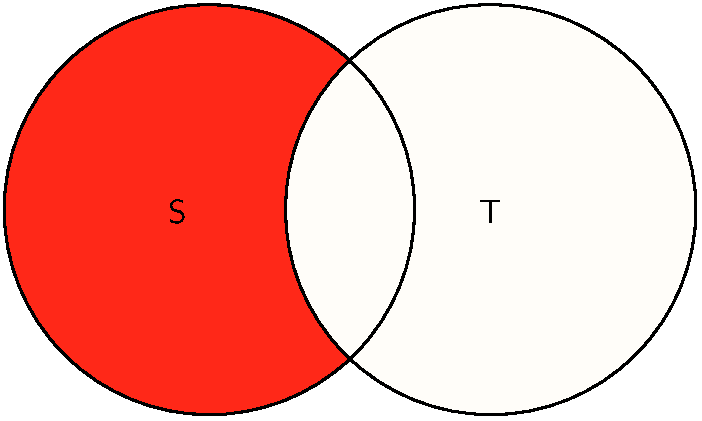
\includegraphics[scale=0.4]{img/difference.pdf}
		\end{figure}
	\end{column}
\end{columns}
\end{frame}

\begin{frame}\frametitle{\insertsection}
	\framesubtitle{\insertsubsection}
   \structure{Beispiel für die Differenzoperation}
\begin{center}
\begin{tabular}{|c|c|c|}\hline
				\multicolumn{2}{|c|}{\footnotesize \textbf{Kunde(S)}}\\\hline\hline
				 \footnotesize \textbf{\key{KNR}} &  \footnotesize \textbf{Nachname}  \\\hline
				\footnotesize 1 &\footnotesize Musterfrau \\\hline
				\footnotesize 2 &\footnotesize  Mustermann  \\\hline
				$\cdots$ &  $\cdots$  \\\hline
			\end{tabular}
			$-$
			\begin{tabular}{|c|c|c|}\hline
				\multicolumn{2}{|c|}{\footnotesize \textbf{Kunde(T)}}\\\hline\hline
				 \footnotesize \textbf{\key{KNR}}  & \footnotesize \textbf{Nachname}  \\\hline
				\footnotesize 1 &\footnotesize Musterfrau \\\hline
				\footnotesize 42 &\footnotesize  Meiser  \\\hline
				$\cdots$ & $\cdots$  \\\hline
			\end{tabular}
			$=$
			\begin{tabular}{|c|c|c|}\hline
				\multicolumn{2}{|c|}{\footnotesize \textbf{Kunde(R)}}\\\hline\hline
				 \footnotesize \textbf{{KNR}} & \footnotesize \textbf{Nachname}  \\\hline
				\footnotesize 2 & \footnotesize  Mustermann  \\\hline
				$\cdots$ & $\cdots$  \\\hline
			\end{tabular}
		\end{center}
\end{frame}

\begin{frame}\frametitle{\insertsection}
\framesubtitle{\insertsubsection}
\onslide
\structure{\textbf{Abgeleitete Operation: Schnitt $\cap$}}
\vspace{5mm}
\begin{columns}
	\begin{column}{.58\textwidth}
		Der Schnitt zweier Relationen $S$ und $T$ aus der gleichen Relationenklasse $\mcl{P}(\mcl{R})$
		besteht aus allen Tupeln, die in $S$ und in $T$ vorkommen.
		\begin{equation*}
		S\cap T=\{r|r\in S \text{\ und\ } r \in T\}
		\end{equation*}
	\end{column}
	\begin{column}{.33\textwidth}
		\begin{figure}
			\vspace{-0.5cm}
			\includegraphics[scale=0.4]{img/intersect.pdf}
		\end{figure}
	\end{column}
\end{columns}
\pause
\abs\abs\abs\abs
Die Schnittoperation leitet sich aus der Differenzoperation ab: $S\cap T = S-(S-T)$.\\
\end{frame}

\begin{frame}\frametitle{\insertsection}
\framesubtitle{\insertsubsection}
\structure{Beispiel für die Schnittoperation}
\begin{center}
\begin{tabular}{|c|c|c|}\hline
				\multicolumn{2}{|c|}{\footnotesize \textbf{Kunde(S)}}\\\hline\hline
				 \footnotesize \textbf{\key{KNR}} &  \footnotesize \textbf{Nachname}  \\\hline
				\footnotesize 1 &\footnotesize Musterfrau \\\hline
				\footnotesize 2 &\footnotesize  Mustermann  \\\hline
				$\cdots$ &  $\cdots$  \\\hline
			\end{tabular}
			$\cap$
			\begin{tabular}{|c|c|c|}\hline
				\multicolumn{2}{|c|}{\footnotesize \textbf{Kunde(T)}}\\\hline\hline
				 \footnotesize \textbf{\key{KNR}}  & \footnotesize \textbf{Nachname}  \\\hline
				\footnotesize 1 &\footnotesize Musterfrau \\\hline
				\footnotesize 42 &\footnotesize  Meiser  \\\hline
				$\cdots$ & $\cdots$  \\\hline
			\end{tabular}
			$=$
			\begin{tabular}{|c|c|c|}\hline
				\multicolumn{2}{|c|}{\footnotesize \textbf{Kunde(R)}}\\\hline\hline
				 \footnotesize \textbf{{KNR}} & \footnotesize \textbf{Nachname}  \\\hline
				\footnotesize 1 & \footnotesize  Musterfrau  \\\hline
				$\cdots$ & $\cdots$  \\\hline
			\end{tabular}
		\end{center}
\end{frame}

\begin{frame}[label=cartProd]\frametitle{\insertsection}
\framesubtitle{\insertsubsection}
\structure{\textbf{Das kartesische Produkt $\times$}}\\[8pt]
$S$ Relation des Schemas $\mcl{R}_1(N\mid A_1,\ldots , A_n)$\\[4pt]
$T$ Relation des Schemas $\mcl{R}_2(N^\prime\mid B_1,\ldots , B_m)$\\[8pt]
Dann ist das kartesische Produkt $S\times T$ die Relation
\begin{equation*}
S\times T = \{(s_1,\ldots,s_n,t_1,\ldots,t_m) \mid (s_1,\ldots s_n) \in S \text{ und } (t_1,\ldots,t_m) \in T \}
\end{equation*}
des Schemas $\mcl{R}_3(N N^\prime\mid A_1,\ldots , A_n,B_1,\ldots ,B_m)$.
\end{frame}

\begin{frame}
\frametitle{\insertsection}
\framesubtitle{\insertsubsection}
\onslide 
\structure{\textbf{Kartesische Produkt $\times$}}\\[8pt]
\begin{itemize}
\item In $S\times T$ werden alle Tupel aus $S$ mit allen Tupeln aus $T$ kombiniert (konkateniert).\\[4pt]
\item Das Ergebnis besteht daher aus $\vert S\vert\cdot\vert T\vert$ Tupeln.\\[8pt]
\pause
\item Ambivalenz:
\begin{itemize}
	\item Falls $\mcl{R}_1$ und $\mcl{R}_2$ gleichnamiges Attribut $A$ haben:\\
	Identifikation bspwse.~durch Relationennamen $N$ und $N^\prime$ {gem\"a\ss} $N.A$ bzw.~$N^\prime.A$\\[8pt]
	\item Dazu sp\"ater mehr.
\end{itemize}
\end{itemize}
\end{frame}

\begin{frame}\frametitle{\insertsection}
\framesubtitle{\insertsubsection}
\structure{Verknüpfung zweier Relationen mit dem kartesischen Produkt}\\[8pt]
Ausgangstabellen:
\begin{columns}
	\begin{column}{.35\textwidth}
		\begin{center}
			\begin{tabular}{|c|c|c|}\hline
				\multicolumn{3}{|c|}{\footnotesize \textbf{Kunde}}\\\hline\hline
				\footnotesize \textbf{\key{KNR}} & \footnotesize \textbf{Vorname} & \footnotesize \textbf{Nachname}  \\\hline
				\footnotesize 1 &\footnotesize Elsa &\footnotesize Musterfrau \\\hline
				\footnotesize 2 & \footnotesize Max &\footnotesize  Mustermann  \\\hline
			\end{tabular}
		\end{center}
	\end{column}
	$\times\quad$
	\begin{column}{.35\textwidth}
		\begin{center}
			\begin{tabular}{|c|c|}\hline
				\multicolumn{2}{|c|}{\footnotesize \textbf{Auftrag}}\\\hline\hline
				\footnotesize \textbf{\key{ANR}} & \footnotesize \textbf{Datum}  \\\hline
				\footnotesize 1001 &\footnotesize 02.01.2013 \\\hline
				\footnotesize 1002 &\footnotesize  04.05.2013  \\\hline
			\end{tabular}
		\end{center}
	\end{column}
\end{columns}
%	\vspace{5mm}
%	Die Relationen sollen mittels des kartesischen Produktes miteinander verknüpft werden.
%	\alert{Achtung: Die Relationenschemata müssen paarweise disjunkt sein, es dürfen daher keine gleichnamigen Attribute existieren!
%	Ergebnis: Siehe Folie \ref{frame:kartesischesProduktErgebnis}.}
\end{frame}

\begin{frame}\label{frame:kartesischesProduktErgebnis}
\frametitle{\insertsection}
\framesubtitle{\insertsubsection}
\structure{Verknüpfung zweier Relationen mit dem kartesischen Produkt}\\[8pt]
	Ergebnisrelation:
	\begin{center}
		\begin{tabular}{|c|c|c|c|c|}\hline
			\multicolumn{5}{|c|}{\footnotesize \textbf{Kunde $\times$ Auftrag}}\\\hline\hline
			\footnotesize{\textbf{KNR}} & \footnotesize{\textbf{Vorname}} & \footnotesize{\textbf{Nachname}} 
			  &\footnotesize{\textbf{ANR}} & \footnotesize{\textbf{Datum}}\\\hline
			1 & Elsa & Musterfrau & 1001  & 02.01.2013\\\hline
			1 & Elsa & Musterfrau & 1002 & 04.05.2013\\\hline
			2 & Max & Mustermann & 1001  & 02.01.2013\\\hline
			2 & Max & Mustermann & 1002  & 04.05.2013\\\hline
		\end{tabular}
	\end{center}
	Jedem Kunden wird jeder Auftrag zugeordnet, was semantisch keinen Sinn ergibt.\\
	Es werden \textit{unechte Tupel} erzeugt $\rightarrow$ dazu später mehr
\end{frame}

\begin{frame}\frametitle{\insertsection}
\framesubtitle{\insertsubsection}
\onslide
\structure{\textbf{Umbenennung}}\\[8pt]
Problemstellung:
\begin{itemize}
	\item Ambivalenz der Namensgebung von Attributen gleichen Namens im kartesischen Produkt 
	\item Semantische Bedeutung von Daten oft mit dem Attributnamen assoziiert
	\item Namen k\"onnen aber obsolet werden\\[8pt]
\end{itemize}
\pause
Ziel:
\begin{itemize}
	\item Operation benötigt, mit deren Hilfe man diesen Umst\"anden Rechnung tragen kann
	\item Datenstruktur des Schemas darf von dieser Operation nicht betroffen sein
\end{itemize}
\end{frame}

\begin{frame}\frametitle{\insertsection}
\framesubtitle{\insertsubsection}
\structure{\textbf{Umbenennung}}\\[8pt]
\begin{block}{}
	Umbenennung von Namen eines Schemas oder von Attributen eines Schemas:
	\begin{itemize}
		\item	Transformation des Schemas $\mcl{R}$ in ein Schema $\mcl{R}^\prime$ mit gleicher Datenstruktur
		\item Erzeugt aus einer Relation $S$ von $\mcl{R}$ eine Relation $S^\prime$ von $\mcl{R}^\prime$
	\end{itemize}
\end{block}
\end{frame}

\begin{frame}\frametitle{\insertsection}
\framesubtitle{\insertsubsection}
\structure{\textbf{Umbenennungsoperation $\rho$}}\\[8pt]
\begin{block}{}
\begin{itemize}
	\item Umbenennung des Attributnamens $A$ in $B$:
	\begin{equation*}
	\rho_{B\leftarrow A}(S)
	\end{equation*} 		
	f\"uhrt Relation $S$ von $\mcl{R}$ in Relation $S^\prime$ \"uber, die Attributnamen $B$ statt $A$ hat.
	\item Umbenennung des Schemanamens $N$ (von Schema $\mcl{R}$) in $N^\prime$ (von Schema $\mcl{R}^\prime$): 
	\begin{equation*}
	\rho_{N^\prime\leftarrow N}(S)
	\end{equation*} 		
	f\"uhrt Relation $S$ von Schema $\mcl{R}$ in Relation $S^\prime$ von Schema $\mcl{R}^\prime$ \"uber, das Schemanamen 
	$N^\prime$ hat.
\end{itemize}
\end{block}
\end{frame}

\begin{frame}\frametitle{\insertsection}
\framesubtitle{\insertsubsection}
\onslide 
\structure{\textbf{Umbenennungsoperation $\rho$}}\\[8pt]
\structure{Beispiel: Umbenennung Attributname}
\begin{center}
S=
\begin{tabular}{|c|c|}\hline
\multicolumn{2}{|c|}{\footnotesize \textbf{Auftrag}}\\\hline\hline
\footnotesize \textbf{\key{ANR}} & \footnotesize \textbf{Datum}  \\\hline
\footnotesize 1001 &\footnotesize 02.01.2013 \\\hline
\footnotesize 1002 &\footnotesize  04.05.2013  \\\hline
\end{tabular}
\pause 
$\quad\quad\rho_{AnNr\leftarrow ANR}(S) =$
\begin{tabular}{|c|c|}\hline
\multicolumn{2}{|c|}{\footnotesize \textbf{Auftrag}}\\\hline\hline
\footnotesize \textbf{\key{AnNr}} & \footnotesize \textbf{Datum}  \\\hline
\footnotesize 1001 &\footnotesize 02.01.2017 \\\hline
\footnotesize 1002 &\footnotesize  04.05.2017  \\\hline
\end{tabular}
\end{center}
\end{frame}

\begin{frame}\frametitle{\insertsection}
\framesubtitle{\insertsubsection}
\onslide 
\structure{\textbf{Umbenennungsoperation $\rho$}}\\[8pt]
\structure{Beispiel: Umbenennung Schemaname}
\begin{center}
S=
\begin{tabular}{|c|c|}\hline
\multicolumn{2}{|c|}{\footnotesize \textbf{Auftrag}}\\\hline\hline
\footnotesize \textbf{\key{ANR}} & \footnotesize \textbf{Datum}  \\\hline
\footnotesize 1001 &\footnotesize 02.01.2013 \\\hline
\footnotesize 1002 &\footnotesize  04.05.2013  \\\hline
\end{tabular}
\pause
$\quad\quad\rho_{Order\leftarrow Auftrag}(S) =$
\begin{tabular}{|c|c|}\hline
\multicolumn{2}{|c|}{\footnotesize \textbf{Order}}\\\hline\hline
\footnotesize \textbf{\key{ANR}} & \footnotesize \textbf{Datum}  \\\hline
\footnotesize 1001 &\footnotesize 02.01.2017 \\\hline
\footnotesize 1002 &\footnotesize  04.05.2017  \\\hline
\end{tabular}
\end{center}
\end{frame}

\begin{frame}
\frametitle{\insertsection}
\framesubtitle{\insertsubsection}
\onslide
\structure{\textbf{Anwendung Umbenennungsoperation $\rho$: \nl Kartesische Produkte von Relationen mit gleichen Attributnamen}}
\abs
Ausgangstabellen:
\begin{columns}
	\begin{column}{.48\textwidth}
		\begin{center}
			\begin{tabular}{|c|c|c|}\hline
				\multicolumn{3}{|c|}{\footnotesize \textbf{Kunde}}\\\hline\hline
				\footnotesize \textbf{\key{KNR}} & \footnotesize \textbf{Vorname} & \footnotesize \textbf{Nachname}  \\\hline
				\footnotesize 1 &\footnotesize Elsa &\footnotesize Musterfrau \\\hline
				\footnotesize 2 & \footnotesize Max &\footnotesize  Mustermann  \\\hline
			\end{tabular}
		\end{center}
	\end{column}
	\begin{column}{.48\textwidth}
		\begin{center}
			\begin{tabular}{|c|c|c|}\hline
				\multicolumn{3}{|c|}{\footnotesize \textbf{Auftrag}}\\\hline\hline
				\footnotesize \textbf{\key{ANR}} & \footnotesize \textbf{KNR}&\footnotesize \textbf{Datum}  \\\hline
				\footnotesize 1001 &\footnotesize 1 &\footnotesize 02.01.2013 \\\hline
				\footnotesize 1002 & \footnotesize 2& \footnotesize  04.05.2013  \\\hline
			\end{tabular}
		\end{center}
	\end{column}
\end{columns}
\abs
\pause
\begin{itemize}
	\item In beiden Relationen existiert das Attribut \texttt{KNR}
	\item Vor Bildung des kartesischen Produktes: Umbenennung der Attribute
	\item Ergebnis: Siehe n\"achste Folie \ref{frame:kartesischesProduktMitUmbenennungErgebnis}.
\end{itemize}
\end{frame}

\begin{frame}	\label{frame:kartesischesProduktMitUmbenennungErgebnis}
\frametitle{\insertsection}
\framesubtitle{\insertsubsection}
\structure{\textbf{Anwendung der Umbenennungsoperation $\rho$: \nl Kartesische Produkte mit Relationen mit gleichen Attributnamen}}
\abs
Ergebnisrelation:
\begin{center}
\begin{tabular}{|c|c|c|c|c|c|}\hline
	\multicolumn{6}{|c|}{\footnotesize \textbf{Kunde $\times$ Auftrag}}\\\hline\hline
	\cellcolor{Yellow}\footnotesize{\textbf{Kunde.KNR}} & \footnotesize{\textbf{Vorname}} & \footnotesize{\textbf{Nachname}} &\footnotesize{\textbf{ANR}} & \cellcolor{Yellow}\footnotesize{\textbf{Auftrag.KNR}}&\footnotesize{\textbf{Datum}}\\\hline
	1 & Elsa & Musterfrau & 1001  & 1 & 02.01.2013\\\hline
	\cellcolor{Red}1 & Elsa & Musterfrau & 1002 &\cellcolor{Red} 2& 04.05.2013\\\hline
	\cellcolor{Red}2 & Max & Mustermann & 1001  &\cellcolor{Red} 1& 02.01.2013\\\hline
	2 & Max & Mustermann & 1002  & 2& 04.05.2013\\\hline
\end{tabular}
\end{center}
\begin{itemize}
\item Nach wie vor werden \backgroundcolour{red}{unechte Tupel} erzeugt, die semantisch nicht zusammen passen. 
\item Auch hierfür gibt es eine Operation, die diesem Umstand begegnet ...
\end{itemize}
\end{frame}

\begin{frame}
\frametitle{\insertsection}
\framesubtitle{\insertsubsection}
\onslide
\structure{\textbf{Selektion $\sigma$}}\\[8pt]
\begin{block}{}
	Selektion von Tupeln einer Relation $R$, die einen Prädikatsausdruck $\theta$ erfüllen.\\
	Ergebnis der Selektionsoperation ist ein Tupel des gleichen Relationenschemas:
	\begin{equation*}
	\sigma_{\theta}(R)=\{t\in R\mid t \text{ erf\"ullt Bedingung } \theta\}
	\end{equation*}
\end{block}
\pause
\abs
Beispiel: $R=Kunde\times Auftrag$, $\theta = (Kunde.KNR=Auftrag.KNR)$
\begin{center}
	\backgroundcolour{green}{$\sigma_{\theta}(R)$} $=$
	\begin{tabular}{|c|c|c|c|c|c|}\hline
		\multicolumn{6}{|c|}{\footnotesize \textbf{Kunde $\times$ Auftrag}}\\\hline\hline
		\footnotesize{\textbf{Kunde.KNR}} & \footnotesize{\textbf{Vorname}} & \footnotesize{\textbf{Nachname}} &\footnotesize{\textbf{ANR}} & \footnotesize{\textbf{Auftrag.KNR}}&\footnotesize{\textbf{Datum}}\\\hline
		\cellcolor{Green}1 &\cellcolor{Green} Elsa & \cellcolor{Green}Musterfrau &\cellcolor{Green} 1001  &\cellcolor{Green} 1 &\cellcolor{Green} 02.01.2013\\\hline
		1 & Elsa & Musterfrau & 1002 &2& 04.05.2013\\\hline
		2 & Max & Mustermann & 1001  &1& 02.01.2013\\\hline
		\cellcolor{Green}2 &\cellcolor{Green} Max & \cellcolor{Green}Mustermann & \cellcolor{Green}1002  & \cellcolor{Green}2&\cellcolor{Green} 04.05.2013\\\hline
	\end{tabular}
\end{center}
\end{frame}

\begin{frame}\frametitle{\insertsection}
\framesubtitle{\insertsubsection}
\structure{\textbf{Im Beispiel: Kombinierte Anwendung}}
\begin{itemize}
	\item Umbenennung: Gemeinsame Attributnamen von zwei Relationen umbenennen\\[5pt]
	\item Kartesisches Produkt: Zwei Relationen vollst\"andig kombinieren 
	\begin{itemize}
		\item unechte Tupel eingeschlossen\\[5pt]
	\end{itemize}
	\item Selektion: Auswahl von Tupeln, die Bedingung (Prädikat) erfüllen
	\begin{itemize}
		\item Selektion echter Tupel m\"oglich
	\end{itemize}
\end{itemize}
\begin{center}
	$\sigma_{\theta}(R)$ $=$
	\begin{tabular}{|c|c|c|c|c|c|}\hline
		\multicolumn{6}{|c|}{\footnotesize \textbf{Kunde $\times$ Auftrag}}\\\hline\hline
		\footnotesize{\textbf{Kunde.KNR}} & \footnotesize{\textbf{Vorname}} & \footnotesize{\textbf{Nachname}} 
		  &\footnotesize{\textbf{ANR}} & \footnotesize{\textbf{Auftrag.KNR}}&\footnotesize{\textbf{Datum}}\\\hline
		1 &Elsa &Musterfrau &1001  &1 &02.01.2013\\\hline
		2 &Max &Mustermann &1002  &2&04.05.2013\\\hline
	\end{tabular}
\end{center}
\end{frame}

\begin{frame}
\frametitle{\insertsection}
\framesubtitle{\insertsubsection}
\onslide
\structure{\textbf{Projektion $\Pi$}}\\[8pt]
\begin{block}{}
	Projektion aller Tupel einer Relation $S$ auf die Attribute einer Attributliste $\{A_1,\dots A_m\}$.\\
	Ergebnis der Projektionsoperation ist eine Relation des projizierten Relationenschemas:
	\begin{equation*}
	\Pi_{\{A_1,\dots A_m\}}(S) = \{\Pi_{\{A_1,\dots A_m\}}(t)\mid t\in S\}
	\end{equation*}
\end{block}
\pause
\abs
Beispiel:
\begin{center}
	$S=$
	\begin{tabular}{|c|c|c|}\hline
		\multicolumn{3}{|c|}{\footnotesize \textbf{Auftrag}}\\\hline\hline
		\footnotesize \textbf{\key{ANR}} & \footnotesize \textbf{KNR}&\footnotesize \textbf{Datum}  \\\hline
		\footnotesize 1001 &\footnotesize 1 &\footnotesize 02.01.2013 \\\hline
		\footnotesize 1002 & \footnotesize 2& \footnotesize  04.05.2013  \\\hline
	\end{tabular}		
	$\quad\Pi_{\{ANR,Datum\}}(S)=$
	\begin{tabular}{|c|c|}\hline
		\multicolumn{2}{|c|}{\footnotesize \textbf{Auftragsdatum}}\\\hline\hline
		\footnotesize \textbf{\key{ANR}} &\footnotesize \textbf{Datum}  \\\hline
		\footnotesize 1001 &\footnotesize 02.01.2013 \\\hline
		\footnotesize 1002 & \footnotesize  04.05.2013  \\\hline
	\end{tabular}
\end{center}
\end{frame}

\begin{frame}\frametitle{\insertsection}
\framesubtitle{\insertsubsection}
\structure{\textbf{Join-Operationen} -- Motivation}\\[8pt]
H\"aufiger Anwendungsfall: 
\begin{itemize}
	\item Kartesisches Produkt einer Relation $S$ eines Prim\"arschemas und einer Relation $R$ eines Fremdschemas
	\item Selektion der Tupel im kartesischen Produkt mit gleichen Werten im Prim\"arschl\"ussel $S.P$ und Fremdschl\"ussel $R.F$
\end{itemize}
\begin{equation*}
\sigma_{(S.P=R.F)}(S\times R)
\end{equation*}
\abs
H\"aufiges Vorkommen dieser Kombination f\"uhrte zur Definition der Join-Operation $\Join$:
\begin{equation*}
S \underset{(S.P = R.F)}{\Join} R := \sigma_{(S.P=R.F)}(S\times R)
\end{equation*}
% 	$$\underset{a \theta b}{S \Join T} \ \mathsf{mit} \ \theta \in \{<,\leq,=,\neq,\geq,>\}, a \in S \wedge b \in T$$
%\vspace{2mm}
%\centerline{$\underset{a \theta b}{S \Join T}$ wird auch $\theta$-Verbund (\textbf{Theta-Join}) genannt}
\end{frame}

\begin{frame}\frametitle{\insertsection}
\framesubtitle{\insertsubsection}
\structure{\textbf{Join-Operationen} -- Motivation}\\[8pt]
Noch einmal das Beispiel:\\ Relationen $Kunde$ und $Auftrag$, Pr\"adikat $\theta = (Kunde.KNR = Auftrag.KNR)$
\begin{center}
	\begin{tabular}{|c|c|c|}\hline
		\multicolumn{3}{|c|}{\footnotesize \textbf{Kunde}}\\ \hline\hline
		\footnotesize \textbf{\key{KNR}} & \footnotesize \textbf{Vorname} & \footnotesize \textbf{Nachname}  \\ \hline
		\footnotesize 1 &\footnotesize Elsa &\footnotesize Musterfrau \\ \hline
		\footnotesize 2 & \footnotesize Max &\footnotesize  Mustermann  \\ \hline
	\end{tabular}
	\hspace{10mm}
	\begin{tabular}{|c|c|c|}\hline
		\multicolumn{3}{|c|}{\footnotesize \textbf{Auftrag}}\\ \hline\hline
		\footnotesize \textbf{\key{ANR}} & \footnotesize \textbf{KNR}&\footnotesize \textbf{Datum}  \\ \hline
		\footnotesize 1001 &\footnotesize 1 &\footnotesize 02.01.2013 \\ \hline
		\footnotesize 1002 & \footnotesize 2& \footnotesize  04.05.2013  \\ \hline
	\end{tabular}
	\abs\abs
	\begin{tabular}{|c|c|c|c|c|c|}\hline
		\multicolumn{6}{|c|}{\footnotesize{ \textbf{Kunde} $\underset{\theta}{\Join}$ \textbf{Auftrag}}}\\\hline\hline
		\footnotesize{\textbf{Kunde.KNR}} & \footnotesize{\textbf{Vorname}} & 
		\footnotesize{\textbf{Nachname}} &\footnotesize{\textbf{ANR}} & 
		\footnotesize{\textbf{Auftrag.KNR}}&\footnotesize{\textbf{Datum}}\\\hline
		1 &Elsa &Musterfrau &1001  &1 &02.01.2013\\\hline
		2 &Max &Mustermann &1002  &2&04.05.2013\\\hline
	\end{tabular}
\end{center}
\end{frame}

\begin{frame}\frametitle{\insertsection}
\framesubtitle{\insertsubsection}
\structure{\textbf{Allgemeine Join-Operationen}}\\[8pt]
\begin{itemize}
	\item Join-Operation nicht nur f\"ur Prim\"ar- und Fremdschl\"usslekombinationen
	\item Join-Operation nicht nur f\"ur Selektion von Tupeln mit gleichen Werten
\end{itemize}
\abs
\textbf{Definition Join-Operation}
\abs
Join-Operation auf Relationen $S$ und $T$ mit beliebigem Selektionspr\"adikat $\theta$:
\begin{equation*}
S \underset{\theta}{\Join} T := \sigma_{\theta}(S\times R)
\end{equation*}
Join-Operation setzt sich aus den elementaren Operationen $\sigma_\theta$ und $\times$ zusammen.
\end{frame}

\begin{frame}\frametitle{\insertsection}
\framesubtitle{\insertsubsection}
\structure{\textbf{Allgemeine Join-Operationen}}\\[8pt]
\begin{alertblock}{Beispiel / \"Ubung}
	\begin{itemize}
		\item Relation $R$ mit Attributen $A_1, A_2,\ldots , A_n$
		\item Relation $S$ mit Attributen $B_1, B_2,\ldots , B_m$
		\item Attribute $A_1$, $A_2$, $A_3$, $B_1$, $B_2$, $B_5$ vom Typ \texttt{integer}
		\item Pr\"adikat $\theta = (A_1 < B_1 \le A_2) \wedge (A_2=B_2) \wedge (A_3 < \frac{1}{2} B_5)$
	\end{itemize}
	\abs
	Beschreiben Sie die Relation $R\underset{\theta}{\Join} S$
\end{alertblock}
\end{frame}

\begin{frame}
\frametitle{\insertsection}
\framesubtitle{\insertsubsection}
\onslide
\structure{\textbf{Equi Join und Natural Join}}\\[8pt]
Besteht $\theta$ eines Join $S \underset{\theta}{\Join} T$
nur aus Gleichheitsaussagen (z.~B.~$\theta = (S.A=T.B) \wedge (S.C=T.D)$), so wird der Join auch 
\textbf{Equi Join} genannt.
\pause
\abs\abs
Werden bei einem Equi Join $S \underset{\theta}{\Join} T$
\begin{itemize}
	\item alle gleichnamigen Attributpaare verkn\"upft 
	\item und in diesem Schema ein Attribut je Attributpaar entfernt,
\end{itemize}
dann nennt man dieses neue Relationenschema \textbf{Natural Join}. Schreibweise: $S \Join T$
\end{frame}

\begin{frame}\frametitle{\insertsection}
\framesubtitle{\insertsubsection}
\structure{\textbf{Equi Join und Natural Join}}\\[8pt]
\begin{alertblock}{Beispiel / \"Ubung}
	\begin{itemize}
		\item Wie sieht ein Equi Join von zwei Relationen aus, die keine paarweise gleichnamigen Attribute haben?\\[6pt]
    %	Existieren keine gleichnamigen Attribute, ist der Natural Join das kartesische Produkt
		\item Beschreiben Sie den Natural Join $S \Join T$ der Relationen $S$ und $T$ mit Attributen $\{A_1,\ldots,A_n,B_1,\ldots, B_m\}$ 
		bzw.~$\{B_1,\ldots, B_m, C_1,\ldots, C_s\}$
		\begin{enumerate}
			\item {\normalsize exemplarisch}\\[4pt]
			\item {\normalsize formal}
		\end{enumerate} 
	\end{itemize}
\end{alertblock}
\end{frame}

\begin{frame}
\frametitle{\insertsection}
\framesubtitle{\insertsubsection}
\onslide
\structure{\textbf{Outer-Join-Operationen}}\\[8pt]
Bisherige Join-Operationen haben nur diejenigen Tupel in die Ergebnisrelation \"uberf\"uhrt, die
\begin{enumerate}
	\item einen entsprechenden Verbundpartner (Tupel) in der anderen Relation haben
	\item die Verbundbedingung $\theta$ erf\"ullt haben
\end{enumerate}
\abs
\pause
Join-Operationen \textbf{Left Outer}, \textbf{Right Outer}, \textbf{Full Outer} enthalten auch Tupel 
\emph{ohne} Verbundpartner:
\begin{itemize}
	\item Left Outer Join $\underset{\theta}\leftouterjoin$ überf\"uhrt \textbf{alle} Tupel der Relation auf der linken Seite des 
	Operators in die Ergebnismenge 
	\item Right Outer Join $\underset{\theta}\rightouterjoin$ überf\"uhrt \textbf{alle} Tupel der Relation auf der rechten Seite 
	des Operators in die Ergebnismenge 
	\item Full Outer Join $\underset{\theta}\fullouterjoin$ ist die Vereinigung von Left und Right Outer Join
\end{itemize}
\end{frame}

\begin{frame}\frametitle{\insertsection}
\framesubtitle{\insertsubsection}
\structure{\textbf{Outer-Join-Operationen} -- Beispiel f\"ur Left Outer Natural Join $\leftouterjoin$}
\begin{center}
	\begin{tabular}{|c|c|c|}\hline
		\multicolumn{3}{|c|}{\footnotesize \textbf{Kunde}}\\\hline\hline
		\footnotesize \textbf{\key{KNR}} & \footnotesize \textbf{Vorname} & \footnotesize \textbf{Nachname}  \\\hline
		\footnotesize 1 &\footnotesize Elsa &\footnotesize Musterfrau \\\hline
		\footnotesize 2 & \footnotesize Max &\footnotesize  Mustermann  \\\hline
		\cellcolor{Yellow}\footnotesize 3 & \cellcolor{Yellow}\footnotesize Hans &\cellcolor{Yellow}\footnotesize Schneider \\\hline
	\end{tabular}
	\hspace{10mm}
	\begin{tabular}{|c|c|c|}\hline
		\multicolumn{3}{|c|}{\footnotesize \textbf{Auftrag}}\\\hline\hline
		\footnotesize \textbf{\key{ANR}} & \footnotesize \textbf{KNR}&\footnotesize \textbf{Datum}  \\\hline
		\footnotesize 1001 &\footnotesize 1 &\footnotesize 02.01.2013 \\\hline
		\footnotesize 1002 & \footnotesize 2& \footnotesize  04.05.2013  \\\hline
	\end{tabular}
	\abs\abs
	\begin{tabular}{|c|c|c|c|c|c|}\hline
		\multicolumn{6}{|c|}{\footnotesize \textbf{Kunde} $\leftouterjoin$ \textbf{Auftrag}}\\\hline\hline
		\footnotesize{\textbf{Kunde.KNR}} & \footnotesize{\textbf{Vorname}} & 
		\footnotesize{\textbf{Nachname}} &\footnotesize{\textbf{ANR}} & 
		\footnotesize{\textbf{Auftrag.KNR}}&\footnotesize{\textbf{Datum}}\\\hline
		\footnotesize 1 & \footnotesize Elsa & \footnotesize Musterfrau &\footnotesize 1001  &\footnotesize 1 &\footnotesize 02.01.2013\\\hline
		\footnotesize 2 & \footnotesize & \footnotesize Mustermann &\footnotesize 1002  &\footnotesize 2& 04.05.2013\\\hline
		\cellcolor{Yellow}\footnotesize 3 &\cellcolor{Yellow}\footnotesize Hans&\cellcolor{Yellow}\footnotesize Schneider
		&\cellcolor{Yellow}\footnotesize\texttt{null}&\cellcolor{Yellow}\footnotesize\texttt{null}
		&\cellcolor{Yellow}\footnotesize\texttt{null}\\\hline
	\end{tabular}
\end{center}
\end{frame}

\begin{frame}
\frametitle{\insertsection}
\framesubtitle{\insertsubsection}
\structure{\textbf{Outer-Join-Operationen}}\\[8pt]
Outer Join-Operationen lassen sich auf die elementaren Operationen 
$\sigma_\theta$, $\times$, $\cup$, $-$, $\Pi$ der relationalen Algebra zur\"uckf\"uhren:
\abs
\begin{theorem}
	\begin{equation*}
	\begin{split}
	R\underset{\theta}\leftouterjoin S &= (R\underset{\theta}\Join S) \cup (R - \Pi_{Attr(R)}(R\Join S)) \times 
	\{\texttt{null},\ldots ,\texttt{null}\}\\
	R\underset{\theta}\rightouterjoin S &= (R\underset{\theta}\Join S)\cup \{\texttt{null},\ldots ,\texttt{null}\}\times 
	(S - \Pi_{Attr(S)}(R\Join S))\\
	R\underset{\theta}\fullouterjoin S &= R\underset{\theta}\leftouterjoin S\cup R\underset{\theta}\rightouterjoin S
	\end{split} 
	\end{equation*}
\end{theorem}
\abs
Beachte: Join-Operation $\underset{\theta}\Join$ setzt sich aus elementaren Operationen $\sigma_\theta$ und $\times$ zusammen.
\end{frame}

\begin{frame}
\frametitle{\insertsection}
\framesubtitle{\insertsubsection}
\structure{\textbf{Aggregation}}\\[8pt]
\begin{itemize}
	\item Aggregation ist ein Operationstyp auf Relationen, 
	der nicht durch die elementaren Operationen der relationalen Algebra ausgedr\"uckt werden kann.
	\item Aggregationen sind somit \textit{nicht} Bestandteil der klassischen relationalen Algebra
	\item Sie wurden als Erweiterung eingef\"uhrt.
	\item Aggregatsfunktionen berechnen aus mehreren (m\"oglicherweise gleichen) Werten einen neuen Wert, das sogenannte Aggregat.
	Beispiele: 
	\begin{itemize}
		\item Summe
		\item Durchschnitt
		\item Minimum oder Maximum
		\item Anzahl
	\end{itemize}
\end{itemize}
\end{frame}

\begin{frame}
\frametitle{\insertsection}
\framesubtitle{\insertsubsection}
\onslide 
\structure{\textbf{Aggregation} -- Motivation}\\[-12pt]
\begin{columns}
	\begin{column}{.3\textwidth}		
		\begin{figure} 
			\includegraphics[scale=0.45]{img/Table_Aggregate_raw.png}\\[-9pt]
			{\tiny Mitarbeiterdaten}
		\end{figure}
	\end{column}
	\pause
	\begin{column}{.3\textwidth}		
		\begin{figure} 
			\includegraphics[scale=0.45]{img/Table_Aggregate_group.png}\\[-9pt]
			{\tiny Mitarbeiter gruppiert nach (Status, Abteilung)}
		\end{figure}
	\end{column}
\end{columns}
\pause 
\begin{figure} 
	\includegraphics[scale=0.45]{img/Table_Aggregate_aggr.png}\\[-8pt]
	{\tiny Mitarbeiterdaten aggregiert nach Gruppen}
\end{figure}
\end{frame}

\begin{frame}
\frametitle{\insertsection}
\framesubtitle{\insertsubsection}
\onslide
\structure{\textbf{Aggregation}}\\[3pt]
\begin{itemize}
	\item $R$ Relation des Schemas $\mcl{R}(G_1,\ldots , G_n, A_1, \ldots , A_m,B_1,\ldots , B_p)$.
	\item Schema $\mcl{R}$ hat Gruppierungsattribute $\{G_1,\ldots , G_n\}$ und Aggregationssattribute $\{A_1,\ldots , A_m\}$
	\begin{itemize}
		\item Im Beispiel: $G_1=\texttt{Status}$, $G_2=\texttt{Abteilung}$, $A_1=\texttt{Gehalt}$, $A_2=\texttt{Jahre}$
	\end{itemize}
	\pause
	\item Datens\"atze in Relation $R$ werden gruppiert nach den unterschiedlichen Werten $(g_1, \ldots , g_n)$ in den Attributen 
	$\{G_1,\ldots , G_n\}$.
	\pause
	\item In jeder dieser Gruppen werden Aggregate aus den Werten der einzelnen Aggregationssattribute $\{A_1,\ldots , A_m\}$
	ermittelt.
	\pause
	\item Neue Tabelle $S$ mit folgenden Spalten: $G_1,\ldots , G_n$, Spalte je Aggregatstyp
	\begin{itemize}
		\item Im Beispiel:
		\nl $G_1=\texttt{Status}$, $G_2=\texttt{Abteilung}$; 
		\nl $\texttt{AVG(Gehalt)}$, $\texttt{MIN(Gehalt)}$, $\texttt{AVG(Jahre)}$ 
	\end{itemize} 
	\pause
	\item Bezeichnung: 
	$S= \Gamma_{\texttt{Status,}\,\texttt{Abteilung\,;}\,
		\texttt{AVG(Gehalt),}\,\texttt{MIN(Gehalt),}\,\texttt{AVG(Jahre)}}(R)$
\end{itemize} 	
\end{frame}

% vvvvvv weglassen vvvvvv
\nowrite{ 
\begin{frame}
\frametitle{\insertsection}
\framesubtitle{\insertsubsection}
\structure{\textbf{Aggregation} -- Notation und formale Beschreibung}\\[3pt]
\begin{itemize}
	\item $R$ Relation des Schemas $\mcl{R}(G_1,\ldots , G_n, A_1, \ldots , A_m,B_1,\ldots , B_p)$.
	\item $R$ partitioniert in (disjunkte) Gruppen $G_{(g_1, \ldots , g_n)}$
	mit Werten $(g_1, \ldots , g_n)$ in den Attributen $(G_1, \ldots , G_n)$.
	\item F\"ur jede Gruppe $G_{(g_1, \ldots , g_n)}\subseteq R$ und zu jedem Attribut $A_i$ ist $ M_{i,(g_1, \ldots , g_n)}$ die Multi-Menge 
	\begin{equation*}
	M_{i,(g_1, \ldots , g_n)} = [x\mid x=\Pi_{A_i}(r) \text{ f\"ur } r \in G_{(g_1, \ldots , g_n)}]
	\end{equation*}
	\item F\"ur jedes aggregierbare Attribut $A_i$ gibt es Aggregationsfunktionen $F^1_i, F^2_i, \ldots , F^{q_i}_i$.
	\item F\"ur jede Gruppe $G_{(g_1, \ldots , g_n)}\subseteq R$ und zu jedem Attribut $A_i$ bilde die Werte 
	\begin{equation*}
	f^1_{i,(g_1, \ldots , g_n)} = F^1_i(M_{i,(g_1, \ldots , g_n)}), \ldots , 
	f^{q_i}_{i,(g_1, \ldots , g_n)} =F^{q_i}_i(M_{i,(g_1, \ldots , g_n)})    
	\end{equation*}
\end{itemize}
\end{frame}
%
\begin{frame}
\frametitle{\insertsection}
\framesubtitle{\insertsubsection}
\structure{\textbf{Aggregation} -- Definition}\\[3pt]
\begin{itemize}
\item $R$ Relation des Schemas $\mcl{R}(G_1,\ldots , G_n, A_1, \ldots , A_m,B_1,\ldots , B_p)$.
%\item Gruppierungsschema: $\mcl{S}(G_1,\ldots , G_n, F^1_1(A_1), \ldots , F^{q_m}_m(A_m))$ 
\item Relation $S$ ist definiert durch % $S$ im Schema $\mcl{S}$
\begin{equation*}
\begin{split}
S=\{t\mid &t=(g_1, \ldots , g_n, f^1_{1,(g_1, \ldots , g_n)}, \ldots f^{q_m}_{m,(g_1, \ldots , g_n)}) \text{ mit }\\
&(g_1, \ldots , g_n) =\Pi_{(G_1,\ldots , G_n)}(r) \text{ f\"ur } r\in R\}
\end{split}
\end{equation*}
\item Relation $S$ ist die \textbf{Aggregation} von $R$ auf den Attributen $A_1, \ldots , A_m$
entlang der Gruppierung $(G_1, \ldots , G_n)$.
\begin{equation*}
\text{Bezeichnung:}\quad\quad\quad\quad\quad\quad S= \Gamma_{G_1, \ldots , G_n; F^1_1(A_1), \ldots , F^{q_m}_m(A_m)}(R)
\phantom{xxxxxxxxxxxxxxxxxxxxxxxxxxxxxxxxxxxxxxxxxx}
\end{equation*}
\end{itemize}
\end{frame}
}
% ^^^^^^ weglassen ^^^^^^

\begin{frame}
\frametitle{\insertsection}
\framesubtitle{\insertsubsection}
\onslide 
\structure{\textbf{Aggregation} -- noch einmal zur\"uck zum Beispiel}
\begin{columns}
	\begin{column}{.3\textwidth}		
		\begin{figure} 
			\includegraphics[scale=0.45]{img/Table_Aggregate_raw.png}\\[-9pt]
			{\tiny Relation Mitarbeiter}
		\end{figure}
	\end{column}
	\pause
	\begin{column}{.6\textwidth}		
		\begin{figure} 
			\includegraphics[scale=0.45]{img/Table_Aggregate_aggr.png}\\[-8pt]
			{\tiny Mitarbeiterdaten aggregiert nach Gruppen}
		\end{figure}
	\end{column}
\end{columns}
\abs\abs
\centering Aggregation: $\Gamma_{\texttt{Status,}\,\texttt{Abteilung\,;}\,
	\texttt{AVG(Gehalt),}\,\texttt{MIN(Gehalt),}\,\texttt{AVG(Jahre)}}(R)$
\end{frame}

% vvvvvv weglassen vvvvvv
\nowrite{ 
\begin{frame}
\frametitle{\insertsection}
\framesubtitle{\insertsubsection}
\structure{Bildung von Aggregaten}
Beispiel: $\Gamma_{KNR, count(*), sum(Wert)}(Auftrag)$
\begin{center}
	\footnotesize
	\begin{tabular}{|c|c|c|}\hline
		\multicolumn{3}{|c|}{\footnotesize \textbf{Auftrag}}\\\hline\hline
		\footnotesize \textbf{\key{ANR}} & \footnotesize{\textbf{KNR}} & \footnotesize \textbf{Wert}  \\\hline
		\footnotesize 1001 & 1 &\footnotesize 10,12 \\\hline
		\footnotesize 1002 & 2 & \footnotesize  12,13  \\\hline
		\footnotesize 1003 & 1 & \footnotesize  14,23  \\\hline
	\end{tabular}
	\hspace{3em}
		\begin{tabular}{|c|c|c|}\hline
			\multicolumn{3}{|c|}{\footnotesize \textbf{$\Gamma_{KNR, count(*), sum(Wert)}(Auftrag)$}}\\\hline\hline
			\footnotesize \textbf{\textbf{KNR}} & \footnotesize{\textbf{count(*)}} & \footnotesize \textbf{sum(Wert)}  \\\hline
			\footnotesize 1 & 2 &\footnotesize 24,35 \\\hline
			\footnotesize 2 & 1 & \footnotesize  12,13  \\\hline
		\end{tabular}
\end{center}
\alert{Nicht-aggregierte Attribute werden als Gruppierungsattribute herangezogen!}
\end{frame}
}
% ^^^^^^ weglassen ^^^^^^

\section*{Übungsaufgaben}
\begin{frame}[t]
	\frametitle{\insertsection}	
	\begin{alertblock}{Relationenmodell und relationale Algebra}
		\begin{enumerate}
			\item Erläutern Sie die Begriffe \emph{Relationenschema} und \emph{Relation eines Relationenschemas}.
			\item Grenzen Sie die Begriffe \textit{funktional abhängig} und \textit{voll funktional abhängig} voneinander ab.
			\item Erläutern Sie den Zusammenhang zwischen funktionaler Abhängigkeit und dem Konzept eines \textit{Schlüssels}.
			\item Für die Identifikation eines Tupels kann jeder Kandidatenschlüssel als Primärschlüssel ausgewählt werden. 
			In welche Situationen könnte einem Kandidatenschlüssel $K_1$ gegenüber einem Kandidatenschlüssel $K_2$ der Vorzug gegeben werden?
			\item Warum ist die Operation $\rho$ essentiell in der relationalen Algebra?
			\item Beschreiben Sie den $\theta$-Join durch elementare Operationen der relationalen Algebra.
			\item Was unterscheidet den Aggregations-Operator $\Gamma$ von den übrigen Operationen der relationalen Algebra?
		\end{enumerate}
	\end{alertblock}
\end{frame}

%!TEX root = Slides.tex

\section{Vom ER-Modell zum relationalen Modell}
\subsection*{Relationen und Attribute}

\begin{frame}[t]
\frametitle{\insertsection}
\framesubtitle{\insertsubsection}
\onslide
Aufgabe: ER-Modelle in relationale Datenmodelle \"uberf\"uhren
\nl
Jedoch einige Besonderheiten bei \"Uberf\"uhrung zu beachten
\pause
\abs
 \begin{itemize}
	\item Entit\"atstypen entsprechen Relationenschemata
	\item Entit\"aten entsprechen Tupeln einer Relation 
	\item Beziehungen k\"onnen ausgedr\"uckt werden durch
	 \begin{itemize}
		\item Fremdschl\"ussel
		\item Relationenschemata
	 \end{itemize}
 \end{itemize}
\end{frame}

\begin{frame}[t]
\frametitle{\insertsection}
\framesubtitle{\insertsubsection}    
\onslide
\structure{Entit\"aten und Attribute i.~d.~R.~direkt in ein Relationenschema \"uberf\"uhrbar:}
\begin{columns}
	\begin{column}{.48\textwidth}			
		\begin{figure}
			\begin{tikzpicture}[node distance=2em]
			\node[entity] (Kunde) {\small Kunde}; 
			\node[attribute] (knr) [above left=2em of Kunde] {\key{\small KNR}} edge (Kunde); 
			\node[attribute] (name) [above right=2em of Kunde] {\small Vorname} edge (Kunde); 
			\node[attribute] (nname) [above=2em of Kunde] {\small Nachname} edge (Kunde); 
			\end{tikzpicture}
		\end{figure}
	\end{column}
	\pause
	$\quad\Longrightarrow$
	\begin{column}{.48\textwidth}
		\begin{center}
			\centerline{\small\texttt{Kunde(\key{KNR},Vorname,Nachname)}}
			\begin{tabular}{|c|c|c|}\hline
				\multicolumn{3}{|c|}{\small \textbf{Kunde}}\\\hline\hline
				\cellcolor{Green}\small \textbf{\key{KNR}} & \small \textbf{Vorname} & \small \textbf{Nachname}  \\\hline 
				\cellcolor{Green}\small 1 &\small Elsa &\small Musterfrau \\\hline 
				\cellcolor{Green}\small 2 & \small Max &\small  Mustermann  \\\hline 
				\cellcolor{Green}\small 3 & \small Hans &\small  Fritsche  \\\hline 
				\cellcolor{Green}$\cdots$ & $\cdots$ & $\cdots$  \\\hline
			\end{tabular}
		\end{center}
	\end{column}
\end{columns}
\abs
\begin{itemize}
	\item Name der Entit\"at wird zum Namen des Relationenschemas.
	\item Attribute werden direkt übernommen. 
	\item Schl\"usseleigenschaften bleiben erhalten.
\end{itemize}
\end{frame}
   
\begin{frame}[t]\frametitle{\insertsection}
\framesubtitle{\insertsubsection}    
\begin{block}{\textbf{Mehrwertige und zusammengesetzte Attribute}}	
	Hierfür im relationalen Datenmodell keine Entsprechung.
	\abs
	Diese Attribute in atomare Attribute auflösen: 
	\begin{itemize}
		\item Zusammengesetzte Attribute: Erzeugung mehrerer Attribute im Relationenschema
		\item Mehrwertige Attribute: Erzeugung eines eigenen Schemas
	\end{itemize}
\end{block}
\end{frame}

\begin{frame}[t]
\frametitle{\insertsection}
\framesubtitle{\insertsubsection}    
\onslide
\structure{Beispiel für mehrwertige Attribute}
\begin{columns}
\begin{column}{0.4\textwidth}
	\begin{figure}
		\scalebox{.8} {
			\begin{tikzpicture}[node distance=2em]
			\node[entity] (Person) {\small Person}; 
			\node[attribute] (mnr) [above left=2em of Person] {\key{\small PNr}} edge (Person); 
			\node[attribute] (name) [above=2em of Person] {\small Name}   edge (Person);
			\node[multi attribute] (title) [above right=2em of Person] {\small Titel} edge (Person); 
			\end{tikzpicture}
		}
	\end{figure}
\end{column}
\pause
$\Longrightarrow\quad\quad$
\begin{column}{0.4\textwidth} 
	\texttt{Person(\key{PNr}, Name)}
	\nl
	\texttt{PersTitel(\key{PNr}(FS), \key{Titel})}	
\end{column}
\end{columns}
\abs\abs\abs
F\"ur das mehrwertige Attribut wird eigenes Relationenschema \texttt{PersTitel} erstellt:
\begin{itemize}
\item Prim\"arschl\"ussel ist Kombination aus dem Attribut selbst und dem Prim\"arschl\"ussel der Ursprungsrelation
\item Prim\"arschl\"ussel der Ursprungsrelation ist Fremdschl\"ussel im neuen Relationenschema
\end{itemize} 
\end{frame}

\subsection{Einfache Beziehungen}

\begin{frame}[t]
\frametitle{\insertsection}
\framesubtitle{\insertsubsection}    
\onslide
\structure{\textbf{(0..1):(0..n)-Beziehungen}}\\[4pt]
\begin{itemize}
	\item Entit\"aten erhalten eigenes Schema
	\item	Beziehung erfordert keine eigene Tabelle
	\item	Prim\"arschl\"ussel der Tabelle der Entit\"at mit (0..1)-Bezeichnung als Fremdschl\"ussel in Tabelle 
	der Entit\"at mit (0..n)-Bezeichnung
\end{itemize}
\begin{columns}
	\begin{column}{0.5\textwidth}
		\begin{figure}
			\scalebox{.6} {
				\begin{tikzpicture}[node distance=2em]
				\node[entity] (Person) {\small Kunde}; 
				\node[attribute] (mnr) [above left=2em of Person] {\key{\small KNR}} edge (Person); 
				\node[attribute] (name) [above=2em of Person] {\small Name}   edge (Person);
				%\node[attribute] (nname) [above right=2em of Person] {\small Nachname}   edge (Person);
				\node[relationship] (erteilt) [right=of Person] {\small{erteilt}} edge  node[auto,swap] {0..1} (Person); 
				\node[entity] (auftrag) [right=of erteilt]  {\small{Auftrag}} edge  node[auto,swap] {0..n}(erteilt);
				\node[attribute] (profnr) [above=of auftrag] {\small{\key{ANR}}} edge (auftrag);
				\node[attribute] (profname) [above right=of auftrag] {\small{Datum}} edge (auftrag);
				\end{tikzpicture}
			}
		\end{figure}		
	\end{column}
	\pause
	\begin{column}{0.45\textwidth}
		Relationenschema:\\
		\texttt{Kunde(\key{KNR},Name)}\\
		\texttt{Auftrag(\key{ANR},KNR(F),Datum)}
	\end{column}
\end{columns}
\end{frame}

\begin{frame}[t]\frametitle{\insertsection}
\framesubtitle{\insertsubsection}    
\structure{\textbf{(0..1):(0..n)-Beziehungen}}\\[4pt]
\structure{Konkrete Abbildung der beiden Relationen}
\begin{columns}
\begin{column}{.48\textwidth}
	\begin{center}
		\begin{tabular}{|c|c|}\hline
			\multicolumn{2}{|c|}{\small \textbf{Kunde}}\\\hline\hline
			\cellcolor{Green}\small \textbf{\key{KNR}} & \small \textbf{Name} \\\hline 
			\cellcolor{Green}\small 1 &\small Musterfrau \\\hline 
			\cellcolor{Green}\small 2 &\small  Mustermann  \\\hline 
			\cellcolor{Green}\small 3 &\small  Fritsche  \\\hline 
			\cellcolor{Green}$\cdots$ & $\cdots$  \\\hline
		\end{tabular}
	\end{center}
\end{column}	
\begin{column}{.48\textwidth}
	\begin{center}
		\begin{tabular}{|c|c|c|}\hline
			\multicolumn{3}{|c|}{\small \textbf{Auftrag}}\\\hline\hline
			\cellcolor{Green}\small \textbf{\key{ANR}} & \cellcolor{Yellow}\small \textbf{KNR} (F) & \small \textbf{Datum}  \\\hline 
			\cellcolor{Green}\small 1001 &\cellcolor{Yellow}\small 1 &\small 02.01.2013 \\\hline 
			\cellcolor{Green}\small 1002 &\cellcolor{Yellow}\small 2 &\small  04.05.2013  \\\hline 
			\cellcolor{Green}\small 1003 &\cellcolor{Yellow}\small 2 &\small  03.01.2014  \\\hline 
			\cellcolor{Green}$\cdots$ & \cellcolor{Yellow}$\cdots$ & $\cdots$  \\\hline
		\end{tabular}
	\end{center}
\end{column}
\end{columns}
\end{frame}

\begin{frame}[t]
\frametitle{\insertsection}
\framesubtitle{\insertsubsection}    
\onslide
\structure{\textbf{1:(0..n)-Beziehungen}}\\[4pt]
\begin{itemize}
	\item Entit\"aten erhalten eigenes Schema
	\item	Beziehung erfordert keine eigene Tabelle
	\item	Prim\"arschl\"ussel der Tabelle der Entit\"at mit 1-Bezeichnung als Fremdschl\"ussel in Tabelle 
	der Entit\"at mit (0..n)-Bezeichnung
	\item Fremdschl\"ussel \texttt{non-null}
\end{itemize}
\begin{columns}
	\begin{column}{0.5\textwidth}
		\begin{figure}
			\scalebox{.6} {
				\begin{tikzpicture}[node distance=2em]
				\node[entity] (Person) {\small Kunde}; 
				\node[attribute] (mnr) [above left=2em of Person] {\key{\small KNR}} edge (Person); 
				\node[attribute] (name) [above=2em of Person] {\small Name}   edge (Person);
				%\node[attribute] (nname) [above right=2em of Person] {\small Nachname}   edge (Person);
				\node[relationship] (erteilt) [right=of Person] {\small{erteilt}} edge  node[auto,swap] {1} (Person); 
				\node[entity] (auftrag) [right=of erteilt]  {\small{Auftrag}} edge  node[auto,swap] {0..n}(erteilt);
				\node[attribute] (profnr) [above=of auftrag] {\small{\key{ANR}}} edge (auftrag);
				\node[attribute] (profname) [above right=of auftrag] {\small{Datum}} edge (auftrag);
				\end{tikzpicture}
			}
		\end{figure}		
	\end{column}
	\pause
	\begin{column}{0.45\textwidth}
		Relationenschema:\\
		\texttt{Kunde(\key{KNR},Vorname,Nachname)}\\
		\texttt{Auftrag(\key{ANR},KNR(F,nn),Datum)}
	\end{column}
\end{columns}
\end{frame}

\begin{frame}[t]
\frametitle{\insertsection}
\framesubtitle{\insertsubsection}    
\onslide
\structure{\textbf{1:(0..1)-Beziehungen}}\\[4pt]
\begin{itemize}
	\item Entit\"aten erhalten eigenes Schema
	\item	Beziehung erfordert keine eigene Tabelle
	\item	Prim\"arschl\"ussel der Tabelle der Entit\"at mit 1-Bezeichnung als Fremdschl\"ussel in Tabelle 
	der Entit\"at mit (0..1)-Bezeichnung
	\item Fremdschl\"ussel \texttt{non-null} und \texttt{unique}
\end{itemize}
\begin{columns}
	\begin{column}{0.5\textwidth}
		\begin{figure}
			\scalebox{.6} {
				\begin{tikzpicture}[node distance=2em]
				\node[entity] (Person) {\small Kunde}; 
				\node[attribute] (mnr) [above left=2em of Person] {\key{\small KNR}} edge (Person); 
				\node[attribute] (name) [above=2em of Person] {\small Name}   edge (Person);
				%\node[attribute] (nname) [above right=2em of Person] {\small Nachname}   edge (Person);
				\node[relationship] (erteilt) [right=of Person] {\small{erteilt}} edge  node[auto,swap] {1} (Person); 
				\node[entity] (auftrag) [right=of erteilt]  {\small{Auftrag}} edge  node[auto,swap] {0..1}(erteilt);
				\node[attribute] (profnr) [above=of auftrag] {\small{\key{ANR}}} edge (auftrag);
				\node[attribute] (profname) [above right=of auftrag] {\small{Datum}} edge (auftrag);
				\end{tikzpicture}
			}
		\end{figure}		
	\end{column}
	\pause
	\begin{column}{0.45\textwidth}
		Relationenschema:\\
		\texttt{Kunde(\key{KNR},Vorname,Nachname)}\\
		\texttt{Auftrag(\key{ANR},KNR(F,nn,u),Datum)}
	\end{column}
\end{columns}
\end{frame}

\begin{frame}[t]
\frametitle{\insertsection}
\framesubtitle{\insertsubsection}    
\onslide
\structure{\textbf{(0..1):(0..1)-Beziehungen}}\\[4pt]
\begin{itemize}
	\item Entit\"aten erhalten eigenes Schema
	\item	Beziehung erfordert keine eigene Tabelle
	\item	Prim\"arschl\"ussel der Tabelle einer der Entit\"aten als Fremdschl\"ussel in Tabelle 
	der anderen Entit\"at
	\item Fremdschl\"ussel \texttt{unique}
\end{itemize}
\begin{columns}
	\begin{column}{0.5\textwidth}
		\begin{figure}
			\scalebox{.6} {
				\begin{tikzpicture}[node distance=2em]
				\node[entity] (Person) {\small Kunde}; 
				\node[attribute] (mnr) [above left=2em of Person] {\key{\small KNR}} edge (Person); 
				\node[attribute] (name) [above=2em of Person] {\small Name}   edge (Person);
				%\node[attribute] (nname) [above right=2em of Person] {\small Nachname}   edge (Person);
				\node[relationship] (erteilt) [right=of Person] {\small{erteilt}} edge  node[auto,swap] {0..1} (Person); 
				\node[entity] (auftrag) [right=of erteilt]  {\small{Auftrag}} edge  node[auto,swap] {0..1}(erteilt);
				\node[attribute] (profnr) [above=of auftrag] {\small{\key{ANR}}} edge (auftrag);
				\node[attribute] (profname) [above right=of auftrag] {\small{Datum}} edge (auftrag);
				\end{tikzpicture}
			}
		\end{figure}		
	\end{column}
	\pause
	\begin{column}{0.45\textwidth}
		Relationenschema:\\
		\texttt{Kunde(\key{KNR},Vorname,Nachname)}\\
		\texttt{Auftrag(\key{ANR},KNR(F,u),Datum)}
	\end{column}
\end{columns}
\end{frame}

\begin{frame}[t]\frametitle{\insertsection}
\framesubtitle{\insertsubsection}    
\onslide
\structure{\textbf{(0..n):(0..m)-Beziehungen}}\\[4pt]
\begin{itemize}
	\item Entit\"aten erhalten eigenes Schema
	\item Beziehung wird zu eigenem Schema
	\begin{itemize}
		\item Der Prim\"arschl\"ussel besteht aus den Prim\"arschl\"usseln der Schemata der Entit\"aten
		\item Die Prim\"arschl\"ussel der Schemata der Entit\"aten sind Fremdschl\"ussel
		\item Ggf.~Attribute der Beziehung in das Schema der Beziehung aufnehmen
	\end{itemize}
\end{itemize}
\pause
\begin{columns}
	\begin{column}{0.5\textwidth}
		\begin{figure}
			\scalebox{.6} {
				\begin{tikzpicture}[node distance=2em]
				\node[entity] (Person) {\small Person}; 
				\node[attribute] (mnr) [above left=2em of Person] {\key{\small PNr}} edge (Person); 
				\node[attribute] (name) [above=2em of Person] {\small Name}   edge (Person);
				\node[relationship] (besitzt) [right=of Person] {\small{arbeitet an}} edge  node[auto,swap] {0..m} (Person); 
				\node[entity] (fuehrer) [right=of besitzt]  {\small{Projekt}} edge  node[auto,swap] {0..n} (besitzt);
				\node[attribute] (profnr) [above=of fuehrer] {\small{\key{ProNr}}} edge (fuehrer);
				\node[attribute] (profname) [above right=of fuehrer] {\small{Thema}} edge (fuehrer);
				\end{tikzpicture}
			}
		\end{figure}		
	\end{column}
	\begin{column}{0.35\textwidth}
		\small
		Relationenschema:\\
		\texttt{Person(\key{PNR},Name)}\\
		\texttt{Projekt(\key{ProNr},Thema)}\\
		\texttt{Arbeitet\_An(\key{PNR}(F),\key{ProNr}(F))}
	\end{column}
\end{columns}
\end{frame}

\begin{frame}[t]\frametitle{\insertsection}
\framesubtitle{\insertsubsection}    
\onslide
\structure{\textbf{(0..n):(0..m)-Beziehungen}}\\[4pt]
 \begin{columns}
	\begin{column}{.33\textwidth}
		\begin{center}
			\begin{tabular}{|c|c|}\hline
				\multicolumn{2}{|c|}{\small \textbf{Person}}\\\hline\hline
				\cellcolor{Green}\small \textbf{\key{PNR}} & \small \textbf{Name}  \\\hline 
				\cellcolor{Green}\small 1 &\small Mustermann \\\hline 
				\cellcolor{Green}\small 2 & \small Musterfrau  \\\hline 
				\cellcolor{Green}\small 3 & \small Fritsch   \\\hline 
				\cellcolor{Green}$\cdots$ & $\cdots$ \\\hline
			\end{tabular}
		\end{center}
	\end{column}	
	\begin{column}{.33\textwidth}
		\begin{center}
			\begin{tabular}{|c|c|}\hline
				\multicolumn{2}{|c|}{\small \textbf{Arbeitet\_An}}\\\hline\hline
				\cellcolor{Green}\small \textbf{\key{PNR}(F)} & \cellcolor{Green}\small \textbf{\key{ProNr}(F)}  \\\hline 
				\cellcolor{Green}\small 1 &\cellcolor{Green}\small 1001 \\\hline 
				\cellcolor{Green}\small 1 &\cellcolor{Green}\small 1002 \\\hline 
				\cellcolor{Green}\small 2 &\cellcolor{Green}\small 1002 \\\hline 
				\cellcolor{Green}\small 2 &\cellcolor{Green}\small 1001 \\\hline 				
			\end{tabular}
		\end{center}
	\end{column}	
	\begin{column}{.33\textwidth}
		\begin{center}
			\begin{tabular}{|c|c|}\hline
				\multicolumn{2}{|c|}{\small \textbf{Projekt}}\\\hline\hline
				\cellcolor{Green}\small \textbf{\key{ProNr}} & \small \textbf{Thema}  \\\hline 
				\cellcolor{Green}\small 1001 &\small Entwicklung \\\hline 
				\cellcolor{Green}\small 1002 &\small Marketing \\\hline 
				\cellcolor{Green}\small 1003 &\small Innovation \\\hline 
				\cellcolor{Green}$\cdots$ & $\cdots$  \\\hline
			\end{tabular}
		\end{center}
	\end{column}
\end{columns}
\vspace{5mm}
Relation \texttt{Arbeitet\_An} hat Fremdschl\"ssel auf Relationen der Entit\"aten.\\
Kombination dieser Fremdschl\"ussel ist Prim\"arschl\"ussel von Relation \texttt{Arbeitet\_An}.\\
\end{frame}

\begin{frame}[t]
\frametitle{\insertsection}
\framesubtitle{\insertsubsection}    
\structure{\textbf{1:1-Beziehungen}}\\[4pt]
\structure{Zwei Alternativen:}\\[2pt]
\begin{enumerate}
	\item Beide Entit\"aten werden in einem Relationenschema identifiziert
	\item Jede Entit\"at hat ihr eigenes Relationenschema
\end{enumerate}
\end{frame}

\begin{frame}[t]
\frametitle{\insertsection}
\framesubtitle{\insertsubsection}    
\onslide
\structure{\textbf{1:1-Beziehungen} -- Alternative 1}\\[4pt]
\begin{itemize}
\item Ein Relationenschema
\item Prim\"arschl\"ussel identifiziert eine der beiden Entit\"aten.
\item Zus\"atzliches \texttt{non-null}, unique Attribut identifiziert zweite Entit\"at
\end{itemize}
\pause
\structure{Beispiel:}
\begin{figure}
\scalebox{.6} {
	\begin{tikzpicture}[node distance=2em]
	\node[entity] (Person) {\small Person}; 
	\node[attribute] (mnr) [above left=2em of Person] {\key{\small PNr}} edge (Person); 
	\node[attribute] (name) [above=2em of Person] {\small Name}   edge (Person);
	\node[relationship] (besitzt) [right=of Person] {\small{besitzt}} edge  node[auto,swap] {1} (Person); 
	\node[entity] (aws) [right=of besitzt]  {\small{Ausweis}} edge  node[auto,swap] {1} (besitzt);
	\node[attribute] (profnr) [above=of aws] {\small{\key{ANr}}} edge (aws);
	\node[attribute] (profname) [above right=of aws] {\small{PLZ}} edge (aws);
	\end{tikzpicture}
}  
\end{figure}		
\hspace*{8.5em}\texttt{PersonAusweis(\key{PNr},ANr(nn,u),Name,PLZ)}
\end{frame}

\begin{frame}[t]
\frametitle{\insertsection}
\framesubtitle{\insertsubsection}    
\onslide
\structure{\textbf{1:1-Beziehungen} -- Alternative 2}\\[4pt]
\begin{itemize}
\item Jede Entit\"at erh\"alt eigenes Schema
\item Prim\"arschl\"ussel der beiden Tabellen sind jeweils Fremdschl\"ussel in der anderen Tabelle
\item Fremdschl\"ussel sind \texttt{non-null}
\end{itemize}
\pause
\structure{Beispiel:}
\begin{columns}
\begin{column}{0.55\textwidth}
\begin{figure}
	\scalebox{.6} {
		\begin{tikzpicture}[node distance=2em]
		\node[entity] (Person) {\small Person}; 
		\node[attribute] (mnr) [above left=2em of Person] {\key{\small PNr}} edge (Person); 
		\node[attribute] (name) [above=2em of Person] {\small Name}   edge (Person);
		\node[relationship] (besitzt) [right=of Person] {\small{besitzt}} edge  node[auto,swap] {1} (Person); 
		\node[entity] (aws) [right=of besitzt]  {\small{Ausweis}} edge  node[auto,swap] {1} (besitzt);
		\node[attribute] (profnr) [above=of aws] {\small{\key{ANr}}} edge (aws);
		\node[attribute] (profname) [above right=of aws] {\small{PLZ}} edge (aws);
		\end{tikzpicture}
	}  
\end{figure}		
\end{column}
\begin{column}{0.4\textwidth}
\texttt{Person(\key{PNr},ANr(F,nn),Name)}\\
\texttt{Ausweis(\key{ANr},PNr(F,nn),PLZ)}
\end{column}
\end{columns}
\pause
\abs
\centering\textbf{VORSICHT Deadlock!}
%
% Lösung: Setze beide Foreign-Key Constraints auf <deferrable> / <deferred>
%         Dadurch können beide Inserts/Delets/Updates konsistent in (nach Abarbeitung) 
%         einer Transaktion durgeführt werden.
%
\end{frame}

\subsection{Schwache Entit\"aten}

\againframe<3>{weakentity}

\begin{frame}[t]
\frametitle{\insertsection}
\framesubtitle{\insertsubsection}    
\onslide
{\structure{\textbf{Schwache Beziehungen}\\[4pt]}}
\begin{figure}
	\scalebox{.7}{
		\begin{tikzpicture}[node distance=2em]
		\node[entity] (geb) {\small Geb\"aude}; 
		\node[attribute] (gnr) [above left=2em of geb] {\key{\small GNR}} edge (geb); 
		\node[attribute] (ort) [above=2em of geb] {\small Name} edge (geb);
		\node[ident relationship] (besitzt) [right=of geb] {\small{besitzt}} edge node[auto,swap] {1} (geb); 
		\node[weak entity] (raum) [right=of besitzt]  {\small{Raum}} edge [total] node[auto,swap] {n} (besitzt); 
		\node[attribute] (rnr) [above=of raum] {\small{RNR}} edge (raum);
		\node[attribute] (profname) [above right=of raum] {\small{Groesse}} edge (raum);
		\end{tikzpicture}}
\end{figure}		
\pause[3]
\hspace*{8em}\texttt{Gebäude(\key{GNR},Name)}
\hspace*{2em}\texttt{Raum(\key{GNR}(F),\key{RNR},Groesse)}
\pause[2]
\abs
\begin{itemize}
	\item F\"ur beide Entit\"atstypen wird Relationenschema erzeugt.
	\item Prim\"arschl\"ussel im schwachen Schema besteht aus Fremdschl"ussel zum Eigent\"umerschema und 
	entit\"ats-differenzierendem Attribut
\end{itemize}
\end{frame}

\subsection{Beziehungen h\"oheren Grades}

\begin{frame}[t]
\frametitle{\insertsection}
\framesubtitle{\insertsubsection}    
\onslide
\structure{\textbf{Beziehungen vom Grad $n > 2$}}\\[4pt]
\structure{Beispiel}\\[-20pt]
\begin{columns}
	\begin{column}{.5\textwidth}
		\begin{figure}
			\scalebox{.6}{
				\begin{tikzpicture}[node distance=2em]
				\node[entity] (Professor) {\small Professor}; 
				\node[attribute] (pnr) [below left=of Professor] {\small{\key{PNR}}} edge (Professor);
				\node[relationship] (liest) [right=of Professor] {\small{betreut}} edge node[auto,swap] {0..1}  (Professor); 
				\node[entity] (Vorlesung) [right=of liest]  {\small{Student}} edge node[auto,swap] {0..n}  (liest);
				\node[attribute] (vnr) [below right=of Vorlesung] {\small{\key{SNR}}} edge (Vorlesung);
				\node[entity] (thm) [below=of liest] {\small{Thema}} edge node[auto,swap] {0..m} (liest); 
				%\node[attribute] (datum) [below left=of liest] {\small{{Note}}} edge (liest);
				\node[attribute] (rnr) [right=of thm] {\small{\key{TNR}}} edge (thm);
				\end{tikzpicture}
			}
		\end{figure}		
	\end{column}
	\pause[3]
	\begin{column}{.38\textwidth}	
		\small{\\[10pt]\texttt{Student(\key{SNR},...)}\\
			\texttt{Thema(\key{TNR},...)} \\
			\texttt{Professor(\key{PNR},...)}\\
			\texttt{Betreuen(\key{SNR}(F),\key{TNR}(F),PNR(F))}}
	\end{column}
\end{columns}
\pause[2]
\abs
\begin{itemize}
	\item Schema f\"ur jede Entit\"at und f\"ur die Beziehung
	\item Prim\"arschl\"ussel der Entit\"atschemata sind Fremdschlüssel im Beziehungsschema
	\item Prim\"arschl\"ussel des Beziehungsschemas besteht aus Prim\"arschlüsseln der Entit\"atschemata mit $(0..n)$-Bezeichnung 		
	%\item Weiterhin beinhaltet Schema des Beziehungstyps dessen Attribute
\end{itemize}
\end{frame}

\subsection{Is-A-Beziehungen}

\begin{frame}[t]
\frametitle{\insertsection}
\framesubtitle{\insertsubsection}    
\structure{Is-A-Beziehungen (vgl. Folie \ref{isarelation}) müssen besonders betrachtet werden}
\begin{figure}\scalebox{0.8}{
	\begin{tikzpicture}[node distance=2em]
	\node[entity] (Auto) {\small Auto}; 
	\node[isa] (ist) [right=of Auto] {\small{is a}} edge (Auto); 
	\node[entity] (fahrzeug) [right=of ist]  {\small{Fahrzeug}} edge  (ist);
	\end{tikzpicture}}
\end{figure}
Die Entitäten können als Klassen in einem objektorientierten Modell aufgefasst werden. 
\abs
Mögliche Ansätze: 
\begin{itemize}
\item \emph{One Table per Class Hierarchy}
\item \emph{One Table per Concrete Class}
\item \emph{One Table per Class}
\end{itemize}
\end{frame}

\begin{frame}<1>[label=isa]
\frametitle{\insertsection}
\framesubtitle{\insertsubsection}
\only<1>{\structure{Beispiel:}}
\only<2>{\structure{Wiederholung von Folie \ref{isa}:}}
\begin{figure}\scalebox{.8} {
\begin{tikzpicture}[node distance=2em]
\node[entity] (Person) {\small Person}; 
\node[attribute] (pnr) [right=of Person] {\small{PNR}} edge (Person);
\node[attribute] (geb) [left=of Person] {\small{Name}} edge (Person);
\node[isa] (ist) [below=of Person] {\small{is a}} edge (Person); 
\node[entity] (Kunde) [below right=of ist]  {\small{Kunde}} edge  (ist);
\node[attribute] (knr) [above right=of Kunde] {\small{KNR}} edge (Kunde);
\node[attribute] (cat) [below right=of Kunde] {\small{Kategorie}} edge (Kunde);
\node[entity] (Mitarbeiter) [below left=of ist] {\small{Mitarbeiter}} edge (ist);
\node[attribute] (mnr) [below left=of Mitarbeiter] {\small{MNR}} edge (Mitarbeiter);
\node[attribute] (login) [above left=of Mitarbeiter] {\small{Login}} edge (Mitarbeiter);
\end{tikzpicture}}
\end{figure}
\end{frame}

\begin{frame}[t]\frametitle{\insertsection}
\framesubtitle{\insertsubsection}    
\onslide
\structure{\textbf{Is-A-Beziehung} -- One Table per Class Hierarchy}\\[4pt]
\begin{itemize}
\item Die Attribute aller Entit\"aten der Klassenhierarchie in ein gemeinsames Relationenschema 
\item Unterscheidung der Entit\"aten durch ein Diskriminator-Attribut	
\end{itemize}
\begin{center}
\begin{tabular}{|c|c|c|c|c|c|c|}\hline
\multicolumn{7}{|c|}{\small \textbf{Personen}}\\\hline\hline
\small \textbf{\key{PNR}} & \textbf{\small Name}&\small \textbf{MNR}&\textbf{Login} &\small \textbf{KNR}&\small \textbf{Kategorie}&\small\textbf{Typ} \\\hline 
\small 1 &\small Mustermann & \small  &\small  &\small 1001 &\small A-Kunde & K\\\hline 
\small 2 &\small Musterfrau & \small 13  &\small emfr &\small  &\small & M \\\hline 
\small 3 &\small Schneider & \small 14  &\small schn  &\small 1002 &\small B-Kunde&B \\\hline 
\end{tabular}
\end{center}
\pause
\begin{itemize}
\item Attribut \texttt{Typ} dient der Unterscheidung zwischen Mitarbeiter (M), Kunde (K), beides (B).
\item Ansatz einfach zu implementieren, provoziert jedoch \texttt{null}-Werte und wird f\"ur komplexere Hierarchien schwer wartbar.
\end{itemize}
\end{frame}

\begin{frame}[t]
\frametitle{\insertsection}
\framesubtitle{\insertsubsection}    
\onslide
\structure{\textbf{Is-A-Beziehung} -- One Table per Concrete Class}\\[4pt]
\structure{Alle konkreten Klassen werden in eigenem Relationenschema abgebildet.}
\begin{center}
\begin{tabular}{|c|c|c|c|}\hline
\multicolumn{4}{|c|}{\small \textbf{Mitarbeiter}}\\\hline\hline
\small \textbf{\key{PNR}} & \textbf{\small Name}&\small \textbf{MNR}&\textbf{Login} \\\hline 
\small 2 &\small Musterfrau & \small 13  &\small emfr  \\\hline 
\small 3 &\small Schneider & \small 14  &\small schn  \\\hline 
\end{tabular}
\hspace{3mm}
\begin{tabular}{|c|c|c|c|}\hline
\multicolumn{4}{|c|}{\small \textbf{Kunde}}\\\hline\hline
\small \textbf{\key{PNR}} & \textbf{\small Name}&\small \textbf{KNR}&\textbf{Kategorie} \\\hline 
\small 1 &\small Mustermann & \small 1001  &\small A-Kunde  \\\hline 
\small 3 &\small Schneider & \small 1002  &\small B-Kunde  \\\hline 
\end{tabular}
\end{center}
\pause
\begin{itemize}
\item Ansatz leicht zu implementieren
\item \texttt{PNR} muss Eindeutigkeit über alle Relationen garantieren (Art Prim\"arschl\"ussel)
\item Es fehlen Ableitungsinformationen, da keine \texttt{Person} existiert	
\end{itemize}
\end{frame}

\begin{frame}[t]
\frametitle{\insertsection}
\framesubtitle{\insertsubsection}    
\onslide
\structure{\textbf{Is-A-Beziehung} -- One Table per Class}\\[4pt]
\structure{Alle Klassen (auch die abstrakten) werden in eigenem Relationenschema abgebildet.}
\begin{center}
\begin{tabular}{|c|c|}\hline
\multicolumn{2}{|c|}{\small \textbf{Person}}\\\hline\hline
\small \textbf{\key{PNR}} & \textbf{\small Name} \\\hline 
\small 1 &\small Mustermann  \\\hline  
\small 2 &\small Musterfrau  \\\hline 
\small 3 &\small Schneider  \\\hline 
\end{tabular}
\hspace{3mm}
\begin{tabular}{|c|c|c|}\hline
\multicolumn{3}{|c|}{\small \textbf{Mitarbeiter}}\\\hline\hline
\small \textbf{\key{PNR}(F)} & \small \textbf{MNR}&\textbf{Login} \\\hline 
\small 2 & \small 13  &\small emfr  \\\hline 
\small 3 & \small 14  &\small schn  \\\hline 
\end{tabular}
\hspace{3mm}
\begin{tabular}{|c|c|c|}\hline
\multicolumn{3}{|c|}{\small \textbf{Kunde}}\\\hline\hline
\small \textbf{\key{PNR}(F)} & \small \textbf{KNR}&\textbf{Kategorie} \\\hline 
\small 1 & \small 1001  &\small A-Kunde  \\\hline 
\small 3 & \small 1002  &\small B-Kunde  \\\hline 
\end{tabular}
\end{center}
\pause
\begin{itemize}
\item \texttt{PNR} muss in allen Relationen vorhanden sein - Prim\"ar- und/oder Fremdschl\"ussel
\item Alle Ableitungsinformationen sind vorhanden
\item Jedoch erhöhter Aufwand nötig, um die einzelnen Tupel mittels Verbundoperationen zusammenzusetzen
\end{itemize}
\end{frame}

\section*{Übungsaufgaben}
\begin{frame}{\insertsection}
\begin{alertblock}{Überführen Sie das ER-Modell in ein logisches Datenmodell.}{
\centering
\scalebox{.65}{
\centering 			
\begin{tikzpicture}[node distance=2em, transform shape]
\node[entity] (Buch) {\small Buch}; 
\node[attribute] (b_bid) [above left=2em of Buch] {\key{\small BID}} edge (Buch);  
\node[attribute] (b_jahr) [left=2em of Buch] {{\small Jahr}} edge (Buch);  
\node[attribute] (b_titel) [below left=2em of Buch] {{\small Titel}} edge (Buch);  

\node[relationship] (r_be) [right=of Buch] {\small of} edge node [auto, swap] {\small 0..1}(Buch); 
\node[entity] (Exemplar) [right=of r_be] {\small Exemplar} edge node [auto, swap] {\small 0..n} (r_be); 
\node[relationship] (r_eapos) [right=of Exemplar] {\small in} edge node [auto,swap] {\small 0..1} (Exemplar); 


\node[weak entity] (Ausleihposition) [right= of r_eapos] {\small AuslPos} edge node[auto,swap] {\small 0..m} (r_eapos); 
\node[attribute] (ap_posnr) [above right=2em of Ausleihposition] {\key{\small PosNr}} edge (Ausleihposition);  
\node[attribute] (ap_rdatum) [right=2em of Ausleihposition] {{\small Rückdatum}} edge (Ausleihposition);  

\node[ident relationship] (r_auslpos) [below=of Ausleihposition] {\small part} edge [total] node [auto, swap] {\small 0..s} (Ausleihposition); 

\node[entity] (Ausleihe) [below= of r_auslpos] {\small Ausleihe} edge node[auto, swap] {\small 0..1} (r_auslpos);
\node[attribute] (a_aid) [above right=2em of Ausleihe] {\key{\small AID}} edge (Ausleihe); 
\node[attribute] (a_datum) [right=2em of Ausleihe] {\key{\small Datum}} edge (Ausleihe);

\node[relationship] (r_writes) [below= of Buch] {\small writes} edge node [auto, swap] {\small 0..p} (Buch); 

\node[entity] (Autor) [below=of r_writes] {\small Autor} edge node [auto,swap] {\small 0..q} (r_writes); 
\node[attribute] (a_auid) [above left=2em of Autor] {\key{\small AuID}} edge (Autor);  
\node[attribute] (a_vn) [left=2em of Autor] {{\small Vorname}} edge (Autor);  		
\node[attribute] (a_nn) [below left=2em of Autor] {{\small Nachname}} edge (Autor);  


\node[attribute] (e_id) [above left=2em of Exemplar] {\key{\small EID}} edge (Exemplar);  
\node[attribute] (e_dat) [above right=2em of Exemplar] {{\small AnschDat}} edge (Exemplar);  

\node[relationship] (r_ka) [left=of Ausleihe] {\small leiht} edge node [auto, swap] {\small 0..r} (Ausleihe); 
\node[entity] (Kunde) [left=of r_ka] {\small Kunde} edge node [auto, swap] {\small 0..1} (r_ka); 

\node[attribute] (k_id) [above left=2em of Kunde] {\key{\small KID}} edge (Kunde);  		
\node[attribute] (k_vn) [above =2em of Kunde] {{\small Vorname}} edge (Kunde);  		
\node[attribute] (k_nn) [above right=2em of Kunde] {{\small Nachname}} edge (Kunde);  					
\end{tikzpicture}}		
}
\end{alertblock}
\textbf{In welchem Punkt könnte dieses Modell noch verfeinert werden?}
\end{frame}

\begin{frame}{\insertsection}
%\framesubtitle{\insertsubsection}
\begin{alertblock}{Welche Fehler wurden bei der Abbildung ins logische Datenmodell gemacht?}
{			
\centering
\scalebox{.65} {
\begin{tikzpicture}[node distance=2em, transform shape]
\node[entity] (Student) {\small A}; 
\node[attribute] (knr) [above left=2em of Student] {\key{\small U}} edge (Student); 
\node[attribute] (name) [above=2em of Student] {\small V} edge (Student);
\node[relationship] (betreut) [right=of Student] {\small{R}} edge node[auto,swap] {0..n} (Student); 
\node[entity] (prof) [right=of betreut]  {\small{B}} edge node[auto,swap] {0..1} (betreut);
\node[attribute] (profnr) [above=of prof] {\small{\key{X}}} edge (prof);
\node[attribute] (profname) [above right=of prof] {\small{Y}} edge (prof);
\node[attribute] (mnr) [above right=of Student] {\small{W}} edge (Student) ;
\end{tikzpicture}
}		
\abs
\small\texttt{A(\uline{U},V,W)}\\
\small\texttt{B(\uline{X},Y,U(F))}\\
\abs
\scalebox{.65} {
\begin{tikzpicture}[node distance=2em, transform shape]
\node[entity] (Student) {\small Angebotskopf}; 
\node[attribute] (knr) [above left=2em of Student] {\key{\small ANr}} edge (Student); 
\node[attribute] (name) [above=2em of Student] {\small Kunde} edge (Student);
\node[ident relationship] (betreut) [right=of Student] {\small{hat}} edge node[auto,swap] {0..1} (Student); 
\node[weak entity] (prof) [right=of betreut]  {\small{Position}} edge [total] node[auto,swap] {0..n} (betreut);
\node[attribute] (profnr) [above=of prof] {\small{\key{PosNr}}} edge (prof);
\node[attribute] (profname) [above right=of prof] {\small{PosText}} edge (prof);
\node[attribute] (mnr) [above right=of Student] {\small{Datum}} edge (Student) ;
\end{tikzpicture}
}
\abs
\small\texttt{Angebotskopf(\uline{ANr},Kunde,Datum)}\\
\small\texttt{Position(\uline{PosNr},PosText)}\\
}
\end{alertblock}	
\end{frame}

%!TEX root = Slides.tex
\part{SQL}
\label{part:sql}

\section{Einf\"uhrung und Grundlagen}

\subsection{Spracheinordnung}

\begin{frame}[t]\frametitle{\insertsection}
\framesubtitle{\insertsubsection}
\begin{itemize}
	\item Bisher: 
	\begin{itemize}
		\item Formale Modelle zur Beschreibung von Datenbanken: ERM, relationale Modelle
		\item Formale Anfragesprache: Relationale Algebra
	\end{itemize}
	\abs
	\item Jetzt: 
	\begin{itemize}
		\item SQL als konkrete Datendefinitions- und -manipulationssprache
		\item F\"ur die praktische Anwendung in relationalen Datenbankmanagementsystemen (RDBMS)
		\item Basierend auf relationalen Modellen und relationaler Algebra
	\end{itemize}	
\end{itemize}
\end{frame}

\begin{frame}[t]\frametitle{\insertsection}
	\framesubtitle{\insertsubsection}
	\structure{\textbf{Geschichte}}\\[4pt]
	\begin{itemize}
		\item Structured Query Language (SQL) wurde in 1970er Jahren von IBM entwickelt
		\item Ursprünglicher Name: Sequel
		\item Entwicklung im Rahmen von IBM System/R
		\item Heute Standard zur Arbeit in RDBMS
		\item Theoretische Grundlage bildet die relationale Algebra
		\item Verschiedene Versionen, etabliert in den Normen ISO/IEC 9075 (Datenbanksprachen)
		\begin{itemize}
			\item SQL89
			\item SQL92
			\item SQL99
		\end{itemize}
		\item Viele proprietäre Erweiterungen und unterschiedliche Dialekte!
	\end{itemize}
\end{frame}

\begin{frame}[t]\frametitle{\insertsection}
\framesubtitle{\insertsubsection}
SQL beinhaltet Befehle und Operationen aus den Bereichen\\[8pt]
\begin{itemize}
	\item Data Definition Language (DDL)\\[4pt]
	\item Data Manipulation Language (DML)
\end{itemize}
\end{frame}

\begin{frame}[t]\frametitle{\insertsection}
\framesubtitle{\insertsubsection}
\onslide
Data Definition Language (DDL): Erzeugen von Schemata (Metadaten)\\[4pt]
\begin{itemize}
\item Relationenschemata und Attributen mit ihren Wertebereichen
\item Beziehungen zwischen Relationenschemata
\item Integrit\"atsbedingungen
\item Berechtigungen und Zugriffe f\"ur Datanbankmanipulationen  
\item Transaktionskontrolle
\end{itemize}
\pause
\abs
Data Manipulation Language (DML): Abfrage und Manipulation von Daten\\[4pt]
\begin{itemize}
\item (C) Erzeugen neuer Datens\"atze / Tupel
\item (R) Lesen (Abfragen) von Datens\"atzen -- Query
\item (U) \"Andern von Datens\"atzen bzw.~Attributwerten
\item (D) L\"oschen von Datens\"atzen
\end{itemize}
\pause
\abs
Au\ss erdem erm\"oglicht SQL die Definition physischer Zugriffspfade (Indizes).
\end{frame}

\begin{frame}[fragile]\frametitle{\insertsection}
\framesubtitle{\insertsubsection}
\structure{SQL ist eine \emph{deskriptive} oder \emph{deklarative} Sprache}	\\[8pt]
\begin{itemize}
	\item Beschreibung des Problems: Was will man erreichen, was soll berechnet werden?
	\item Die Prozedur wird vom System ermittelt: Wie wird das gew\"unschte Ziel erreicht?
\end{itemize}
\end{frame}

\begin{frame}[fragile]\frametitle{\insertsection}
\framesubtitle{\insertsubsection}
\onslide
\begin{columns}
	\begin{column}{.2\textwidth}
\lstset{language=SQL}
\begin{lstlisting}
 SELECT * FROM Kunde 
 WHERE PLZ = 68165;
\end{lstlisting}
	\end{column}
	\begin{column}{.48\textwidth}
		\lstset{language=Java}
\begin{lstlisting}
 kundenListe = ...
 ArrayList<Kunde> result = new ArrayList<>();
 for (Kunde tmpKunde : kundenListe) {
  if (tmpKunde.getPLZ() == 68165)
   result.add(tmpKunde);
  }
 return result;
\end{lstlisting}
	\end{column}
\end{columns}
\begin{itemize}
\item SQL (links): Beschreibt, was das gew\"unschte Ergebnis sein soll. 
\item Java (rechts): Prozedur/Algorithmus wird implementiert, der das Ergebnis herbeif\"uhrt.\\[8pt]
\pause
\item SQL-Befehle k\"onnen daher auf unterschiedliche Arten implementiert werden.
\item Das erm\"oglicht die physische Datenunabh\"angigkeit.
\item Details: siehe Vorlesung \textit{Datenbanktechnik}.
\end{itemize}
\end{frame}

\subsection{Grundlegende Datentypen}

\begin{frame}\frametitle{\insertsection}
	\framesubtitle{\insertsubsection}
	\structure{Eine (kleine) Auswahl der Datentypen}
	\begin{center}
		\begin{tabular}{|c|p{10cm}|}\hline
			 \small \textbf{Bezeichnung} & \small \textbf{Beschreibung} \\\hline
			\small\texttt{bit, bool} & \small Wahrheitswert, 0 oder 1, \textit{wahr} oder \textit{falsch}  \\\hline
			\small\texttt{char(n)} & \small Character-Sequenz mit einer Fixlänge von $n$ Zeichen  \\\hline
			\small\texttt{varchar(n)} & \small Character-Sequenz mit einer Maximallänge von $n$ Zeichen \\\hline
			\small\texttt{int}&\small Ganzzahlen (4 Byte, von -2147483648 -- 2147483647)\\\hline
			\small\texttt{decimal(p,d)}&\small Fixpoint-Zahl mit insgesamt $p$ Stellen, davon $d$ Nachkommastellen\\\hline
			\small\texttt{real,float,double}&\small Floatingpoint-Zahl mit einfacher (32 Bit) oder doppelter (64 Bit) Genauigkeit\\\hline
			\small\texttt{date,time}&\small Datums- und Zeitangaben\\\hline
			\small\texttt{BLOB}&\small Binary Large Object für Binärdaten\\\hline
		\end{tabular}
	\end{center}
\end{frame}

\begin{frame}\frametitle{\insertsection}
	\framesubtitle{\insertsubsection}
	\structure{Besondere Datentypen (proprietär!)}
	\begin{itemize}
		\item \texttt{enum}, um Aufzählungen abzubilden
		\item Geometrische Datentypen (z.B. \texttt{point}, \texttt{circle} oder \texttt{polygon})
		\item Netzwerktypen (z.B. \texttt{ipv4}, \texttt{cidr} oder \texttt{macaddr})
		\item Universally Unique Identifiers (z.B. \texttt{uuid})
		\item Spezielle Datentypen für Volltextsuchen im Bereich des Natural Language Processing (z.B. \texttt{tsvector})
	\end{itemize}
\abs
Jedes RDBMS hat ein eigenes Set von proprietären Datentypen, ledglich die Basisdatentypen sind interoperabel!
\end{frame}

\subsection{\texttt{null}-Werte}

\begin{frame}[t]\frametitle{\insertsection}
\framesubtitle{\insertsubsection}
\onslide
\texttt{null}-Werte k\"onnen in Tabellen vorkommen und k\"onnen dabei unterschiedliche Bedeutung haben:
\begin{itemize}
	\item Es existiert kein Wert
	\item Es k\"onnte ein Wert existieren, der aber (noch) unbekannt ist
	\item Jeder Wert ist m\"oglich
	\item $\dots$ (insgesamt 13 verschiedene Bedeutungen von \texttt{null})
\end{itemize}
\abs
\pause
\alert{Einheitliche Semantik für \texttt{null} existiert somit nicht! 
Daher muss SQL auf spezielle Weise mit \texttt{null} umgehen. Dazu sp\"ater mehr.}
\end{frame}

\section{Einfache SQL-Statements}
\subsection{Relationenschema -- Erzeugung, Update, L\"oschen}

\begin{frame}[fragile]
\frametitle{\insertsection}
\framesubtitle{\insertsubsection}
\structure{\textbf{Erzeugen einer Datenbank innerhalb des Datenbankmanagementsystems}}\\[4pt]
\lstset{language=sql}
\begin{lstlisting}[numbers=none]
CREATE DATABASE <databasename>;
\end{lstlisting}
\abs
In dieser Datenbank k\"onnen nun Datenbankschemata angelegt werden.
\abs\ \abs\ \abs 
\structure{Doku: \href{https://www.postgresql.org/docs/9.6/static/sql-createdatabase.html}{\textcolor{blue}{\underline{PostgreSQL 
				Online Documentation für \texttt{CREATE DATABASE}}}}}
\end{frame}

\begin{frame}[fragile]
\frametitle{\insertsection}
\framesubtitle{\insertsubsection}
\structure{\textbf{Erzeugen eines Datenbankschemas innerhalb der Datenbank}}\\[4pt]
\lstset{language=sql}
\begin{lstlisting}[numbers=none]
CREATE SCHEMA <schemaname>;
\end{lstlisting}
\abs
In diesem Schema k\"onnen nun Tabellen/Relationenschemata angelegt werden.
\abs\ \abs\ \abs 
\structure{Doku: \href{https://www.postgresql.org/docs/current/static/sql-createschema.html}{\textcolor{blue}{\underline{PostgreSQL 
			Online Documentation für \texttt{CREATE SCHEMA}}}}}
\end{frame}

\begin{frame}[fragile]\frametitle{DDL-Statements}
\framesubtitle{Erzeugen einer Relation}
\structure{\textbf{Erzeugen eines Relationenschemas im Datenbankschema}}\\[4pt]
\lstset{language=sql}
\begin{lstlisting}[numbers=none]
CREATE TABLE "<schemaname>"."R" (a1 d1, a2 d2, ... , an dn);
\end{lstlisting}
\begin{itemize}
\item im Datenbankschema \texttt{<schemaname>}
\item mit Attributnamen $\texttt{a1},\dots,\texttt{an}$ (z.B. Vorname, Name, PLZ)
\item und Dom\"anen $\texttt{d1},\dots,\texttt{dn}$, die auf Datentypen des RDBMS aufbauen 
(z.B. \texttt{int, varchar} etc.)
\end{itemize}
\abs\ \abs 
\structure{Doku: \href{https://www.postgresql.org/docs/current/static/sql-createtable.html}{\textcolor{blue}{\underline{PostgreSQL 
		Online Documentation für \texttt{CREATE TABLE}}}}}
\end{frame}

\begin{frame}[fragile]\frametitle{\insertsection}
\framesubtitle{\insertsubsection}
\structure{Beispiel:}\\[4pt]
\begin{columns}
\begin{column}{0.9\textwidth}
	\lstset{language=sql}
\begin{lstlisting}[numbers=none]
CREATE TABLE Film (FilmNr int, Name varchar(50), ErschJahr int, GenreID int);
\end{lstlisting}
\end{column}
\end{columns}
\abs
\begin{itemize}
\item Erzeugung von Relationenschema \texttt{Film}
\item Attribute \texttt{FilmNr} und \texttt{ErschJahr} Ganzzahlen vom Typ \texttt{int}
\item	Attribut \texttt{Name} Unicode-Zeichenkette vom Typ \texttt{varchar(50)} mit max.~50 Zeichen.
\end{itemize}
\abs
\alert{Hier sind weder Prim\"arschl\"ussel noch Nebenbedingungen definiert worden - z.B. dass der Filmname nicht leer sein darf.
SQL bietet diese M\"oglichkeiten f\"ur Integrit\"atsbedingungen.}
\end{frame}

\begin{frame}[fragile]\frametitle{\insertsection}
	\framesubtitle{\insertsubsection}
	\framesubtitle{Integritätsbedingungen}
	\structure{Attribute können Integritätsbedingungen enthalten, die direkt hinter der Datentyp-Deklaration eingefügt werden können:}
	\abs
	\begin{description}[style=multiline,leftmargin=0cm]
		\item[PRIMARY KEY] Definition eines oder mehrerer Attribute als Primärschlüssel
		\item[UNIQUE] Attribute m\"ussen eindeutig sein, sind aber \textit{nicht der Primärschlüssel}
		\item[NOT NULL] Attribut darf nicht \texttt{null} sein
		\item[CHECK] Es kann eine zusätzliche Prüfbedingung angegeben werden (z.B. keine negativen Altersangaben oder Jahreszahlen)
		\item[DEFAULT] Es kann ein Default-Wert für ein Attribut festgelegt werden
		\item[REFERENCES] Setzt eine Fremdschlüssel-Beziehung auf eine andere Relation
	\end{description}
\end{frame}

\begin{frame}[fragile]
\frametitle{\insertsection}
\framesubtitle{\insertsubsection}
structure{Primary Key}
\begin{lstlisting}[xleftmargin=3ex]
CREATE TABLE Film (
  FilmNr int PRIMARY KEY,
  Name varchar(50) NOT NULL,
  ErschJahr int CHECK (ErschJahr > 1900),
  GenreID int REFERENCES Genre(GenreID)
);
		\end{lstlisting}
		\abs
\begin{itemize}
	\item \texttt{FilmNr} Primärschlüssel des Schemas \texttt{Film}
	\item \texttt{Name} darf nicht den Wert \texttt{null} annehmen 
	\item \texttt{ErschJahr} muss mit Werten $> 1900$ belegt sein
	\item \texttt{GenreID} ist Fremdschlüssel auf Schema \texttt{Genre} und ihr Attribut \texttt{GenreID}	
\end{itemize}
\end{frame}

\begin{frame}[fragile]\frametitle{\insertsection}
\framesubtitle{\insertsubsection}
\structure{Integrit\"tsbedingungen mit \texttt{CHECK}}
\begin{itemize}
	\item Vergleichsoperatoren $<,\leq,=,\geq,>$
	\item \texttt{[NOT] IN (<Werteliste>)}
	\item \texttt{[NOT] BETWEEN (<Werteliste>)}
	\item \texttt{[NOT] LIKE (<Textpattern>)}
\end{itemize}
\abs
\structure{Noch ein Beispiel:}
\begin{lstlisting}[xleftmargin=3ex]
CREATE TABLE Ort
 ...
 PLZ int CHECK(VALUE BETWEEN(0 AND 99999)),
 ...
);
\end{lstlisting}
\end{frame}

\begin{frame}[fragile]\frametitle{\insertsection}
	\framesubtitle{\insertsubsection}
	Integritätsbedingungen können auch nachgelagert werden. 
	\nl
	So können z.B. Attribut-übergreifende Bedingungen formuliert werden:
		\lstset{escapeinside={(*@}{@*)}}
		\begin{lstlisting}[xleftmargin=3ex]
CREATE TABLE Raum (
  GebaeudeNr int,
  RaumNr int,
  Groesse int,
  Beschreibung varchar(100),
  PRIMARY KEY(GebaeudeNr, RaumNR), (*@\label{lst:pk}@*)
  FOREIGN KEY (GebaeudeNr) REFERENCES Gebaeude(GebaeudeNr) (*@\label{lst:fk}@*)
);
		\end{lstlisting}
\abs
\begin{itemize}
	\item Zeile \ref{lst:pk}: Deklaration eines zusammengesetzten Primärschlüssels
	\item Zeile \ref{lst:fk}: Foreign Key kann auch mehrere Attribute enthalten: \texttt{REFERENCES}-Syntax wird zur
	\texttt{FOREIGN KEY}-Syntax erweitert
\end{itemize}	
\end{frame}

\begin{frame}[fragile]\frametitle{\insertsection}
\framesubtitle{\insertsubsection}
\structure{\textbf{Fremdschl\"usselbeziehung}}\\[4pt]
\begin{itemize}
	\item DBMS verbietet das Löschen von Datensätzen (in Prim\"artabelle), 
	auf die durch Fremdschlüssel-Beziehung (in Fremdtabelle) 
	referenziert wird.
	\item	Dieses Verhalten kann mit Hilfe der \texttt{FOREIGN KEY}-Deklaration in der Fremdtabelle
	ver\"andert werden.
	\item Zwei Szenarien: \texttt{ON DELETE} und \texttt{ON UPDATE}. 
\end{itemize}
\end{frame}

\begin{frame}[fragile]\frametitle{\insertsection}
\framesubtitle{\insertsubsection}
\structure{\textbf{Fremdschl\"usselbeziehung}}\\[4pt]
\begin{itemize}
\item \texttt{ON DELETE} legt fest, wie auf \emph{Löschoperationen} reagiert wird
\begin{itemize}
	\item \texttt{CASCADE}: Löscht Datensatz in der referenzierenden Tabelle
	\item \texttt{SET NULL / SET DEFAULT}: Setzt das Attribut in der referenzierenden Tabelle auf \texttt{null} bzw. auf Default-Wert
	\item \texttt{NO ACTION}: Erlaubt das Brechen der Fremdschlüsselbeziehung
\end{itemize}
\item \texttt{ON UPDATE} legt fest, wie auf \emph{Updates} reagiert wird.
\begin{itemize}
	\item \texttt{CASCADE}: \'"Andert den Wert des Attributs in der referenzierenden Tabelle
	\item \texttt{SET NULL / SET DEFAULT}: Setzt das Attribut in der referenzierenden Tabelle \texttt{null} bzw. auf einen Default-Wert
	\item \texttt{NO ACTION}: Erlaubt das Brechen der Fremdschlüsselbeziehung
\end{itemize}
\end{itemize}
\end{frame}

\begin{frame}[fragile]\frametitle{\insertsection}
	\framesubtitle{\insertsubsection}
		\structure{Beispiel:}
		\lstset{escapeinside={(*@}{@*)}}
		\begin{lstlisting}[xleftmargin=3ex]
CREATE TABLE Anschrift (
  ...
  FOREIGN KEY (PLZ) REFERENCES Ort(PLZ)
  ON DELETE CASCADE
  ON UPDATE SET NULL
);
		\end{lstlisting}
\abs
\alert{Achtung: 
	\begin{itemize}
	 \item	Das L\"osch- oder Update-Verhalten kann unabh\"angig voneinander gesetzt werden.
	 \item Das L\"osch- oder Update-Verhalten wird in jeder referenzierenden Fremdtabelle 
	 unabh\"angig gesetzt.
  \end{itemize}}
\end{frame}

\begin{frame}[fragile]\frametitle{\insertsection}
	\framesubtitle{\insertsubsection}
\textbf{Relationschemata werden mit dem \texttt{DROP TABLE} Befehl gelöscht.}\\[4pt]
\structure{Beispiel:}
\begin{lstlisting}[xleftmargin=3ex,numbers=none]
DROP TABLE Raum;
\end{lstlisting}
\abs
\begin{itemize}
	\item L\"oschen der Tabelle beinhaltet L\"oschen aller Inhalte
	\item L\"oschen kann nicht r\"uckg\"angig gemacht werden. 
	\item Wird referentielle Integrit\"at gef\"ahrdet, kann Tabelle nicht gel\"oscht werden.	
\end{itemize}
\abs
\alert{Achtung: Die meisten RDBMS fragen vor Befehlsausführung nicht nach! 
 \texttt{DROP TABLE} sollte daher mit Vorsicht angewendet werden.}
\end{frame}

\begin{frame}[fragile]\frametitle{\insertsection}
	\framesubtitle{\insertsubsection}
	\structure{Nachträgliche Änderungen an Tabellen können mit \texttt{ALTER TABLE} 
		durchgeführt werden.}\\[4pt]
\begin{itemize}
	\item Änderungen von Attributen
	\begin{itemize}
		\item \texttt{\textbf{ALTER TABLE} Raum \textbf{ADD COLUMN} Verwendung varchar(20) NOT NULL}
		\item \texttt{\textbf{ALTER TABLE} Raum \textbf{DROP COLUMN} Verwendung}\\[4pt]
	\end{itemize}
	\item Änderungen von Integritätsbedingungen
	\begin{itemize}
		\item \texttt{\textbf{ALTER TABLE} Raum \textbf{ADD PRIMARY KEY}(RaumNr)}
	\end{itemize}
\end{itemize}
\abs
Befehl \texttt{ALTER TABLE} bietet Vielzahl von weiteren M\"oglichkeiten, die je nach 
verwendetem RDBMS stark variieren k\"onnen.
\end{frame}

\subsection{Relationen -- Einf\"ugen, Update, L\"oschen}

\begin{frame}[fragile]\frametitle{\insertsection}
	\framesubtitle{\insertsubsection}
\onslide
	\structure{Datensätze werden in eine Tabelle mit dem Befehl \texttt{INSERT INTO} eingefügt.}
	\begin{block}{Generelle Syntax}
	\texttt{INSERT INTO <tabellenname> [(attributliste)] VALUES (werteliste)}
	\end{block}
\pause
	\begin{itemize}
		\item Optionale Attributliste benennt jedes einzuf\"ugende Attribut 
		\item Reihenfolge von Attribut- und Werteliste müssen übereinstimmen
		\item Nicht angegebene Attribute werden mit \texttt{null} oder Default-Werten belegt
		\item Ohne Attributliste: Insert eines gesamten Tupel $\rightarrow$ in korrekter Reihenfolge!
	\end{itemize}
\end{frame}

\begin{frame}[fragile]\frametitle{\insertsection}
	\framesubtitle{\insertsubsection}
	\textbf{Beispiel}\\[4pt]
  Einf\"ugen in Tabelle \texttt{Person(ID,Vorname,Nachname)}
	\begin{columns}
		\begin{column}{.48\textwidth}
			\lstset{escapeinside={(*@}{@*)}}
		\begin{lstlisting}[xleftmargin=2ex]
INSERT INTO Person (ID, Nachname)
VALUES
(1,"Meier");
		\end{lstlisting}
		\end{column}

		\begin{column}{.48\textwidth}
			\lstset{escapeinside={(*@}{@*)}}
		\begin{lstlisting}[xleftmargin=3ex]
INSERT INTO Person
VALUES
(1,"Hans","Meier");
		\end{lstlisting}
		\end{column}
	\end{columns}
\abs
\begin{itemize}
	\item Linkes Beispiel: Durch Angabe der Attribute \texttt{ID} und \texttt{Nachname} 
		wird der Vorname mit \texttt{null} belegt. 
	\item Rechtes Beispiel: Ohne Attributliste muss zu allen Attributen der Relation ein Wert
	(in der korrekten Reihenfolge) vorkommen.	
\end{itemize}
\end{frame}

\begin{frame}[fragile]\frametitle{\insertsection}
	\framesubtitle{\insertsubsection}
	\structure{In einem SQL-Befehl können auch mehrere Tupel in Tabelle geschrieben werden:}
	\abs
	\begin{lstlisting}[xleftmargin=3ex]
INSERT INTO Person VALUES
  (1,"Hans","Meier"),
  (2,"Freddy","Kronzucker"),
  (3,"Grete","Schneider");
\end{lstlisting}
\abs
Auf diese Weise können interne Performance-Optimierungen bei Insert-Operationen genutzt werden.
\abs
\alert{Achtung: Multiple Inserts werden nicht von allen RDBMS unterstützt.}
\end{frame}

\begin{frame}[fragile]
\frametitle{\insertsection}
\framesubtitle{\insertsubsection}
\onslide
\structure{Datens\"atze können mit \texttt{UPDATE}-Befehl verändert werden.}\\[4pt]
\begin{block}{Allgemeine Syntax}
	\begin{lstlisting}[xleftmargin=3ex]
UPDATE <tabellenname>
SET <attribut>  = <wert>
WHERE <selektionsbedingungen>;
		\end{lstlisting}
	\end{block}
\pause
\begin{itemize}
	\item Ein Update wird immer nur auf genau einer Tabelle ausgeführt
	\item Dabei wird das benannte Attribut mit einem neuen Wert belegt
	\item Mittels einer \texttt{WHERE}-Bedingung kann die relevante Tupelmenge bestimmt werden. Die Selektionsbedingungen können logisch verknüpft werden (AND / OR)
	\item Wird keine \texttt{WHERE}-Bedingung angegeben, so bezieht sich das Update auf \textit{alle} Tupel.
\end{itemize}
\end{frame}

\begin{frame}[fragile]\frametitle{\insertsection}
	\framesubtitle{\insertsubsection}
	\structure{Beispiele f\"ur Update-Operationen}\\[4pt]
Nachname eines Mitarbeiters soll geändert werden.
	\begin{lstlisting}[xleftmargin=3ex]
UPDATE Person
SET Name  = "Mustermann"
WHERE ID = 3;
		\end{lstlisting}
\abs
Alle Mitarbeiter aus Mannheim mit Gehalt unter 20.000 EUR sollen 10\% mehr Gehalt bekommen
	\begin{lstlisting}[xleftmargin=3ex]
UPDATE Mitarbeiter
SET Gehalt  = Gehalt * 1.1
WHERE Gehalt < 20000
AND Ort  = "Mannheim";
		\end{lstlisting}
\end{frame}

\begin{frame}[fragile]
\frametitle{\insertsection}
\framesubtitle{\insertsubsection}
\onslide
\structure{\textbf{Datens\"atze l\"oschen mit \texttt{DELETE}-Befehl}}\\[4pt]
	\begin{block}{Allgemeine Syntax}
	\begin{lstlisting}[xleftmargin=3ex, numbers=none]
DELETE FROM <tabellenname> WHERE <selektionsbedingungen>;
		\end{lstlisting}
	\end{block}
\abs\pause
\begin{itemize}
	\item Delete-Operation wird immer nur auf genau einer Relation ausgeführt
	\item Alle Tupel, die der Selektionsbedingung entsprechen, werden gelöscht
	\item Wird keine \texttt{WHERE}-Bedingung angegeben, so bezieht sich die Operation auf 
	\textit{alle} Tupel
\end{itemize}
\pause
\alert{Die meisten RDBMS fragen nicht nach! Delete-Operation wird sofort ausgeführt.}
\end{frame}

\begin{frame}[fragile]\frametitle{\insertsection}
	\framesubtitle{\insertsubsection}
\structure{Beispiel}\\[4pt]
Alle Kunden aus Mannheim sollen gelöscht werden:
\begin{lstlisting}[xleftmargin=3ex, numbers=none]
DELETE FROM Kunden WHERE Ort =  "Mannheim";
\end{lstlisting}
\end{frame}

\subsection{Abfragen auf Relationen}

\begin{frame}[fragile]
\frametitle{\insertsection}
\framesubtitle{\insertsubsection}
\onslide
	\structure{\textbf{Lesen von Datens\"atzen mit \texttt{SELECT}-Statement}}\\[4pt]
	\begin{block}{Allgemeine Syntax -- wird sp\"ater noch erweitert}
		\begin{lstlisting}[xleftmargin=3ex]
SELECT [DISTINCT] <Attributliste>
FROM <Tabellenliste>
WHERE <Bedingungen>;
		\end{lstlisting}
	\end{block}
\abs\pause
	\begin{itemize}
		\item \texttt{SELECT} umfasst die Operationen Produkt, Selektion, Projektion der 
		relationalen Algebra -- wird sp\"ater noch durch Join-Operation erweitert
		\item Produkt: Aus einer oder mehreren Tabellen aus \texttt{<Tabellenliste>}
		\item Selektion: Selektionsbedingungen werden i.~S.~d.~relationalen Algebra in 
		\texttt{<Bedingungen>} gesetzt
		\item Projektion: Angabe der projizierten Attribute in \texttt{<Attributliste>} ($*$ erlaubt)
		\item Duplikate werden durch optionales \texttt{DISTINCT} eliminiert. Beachte: SQL l\"asst 
		\emph{Multisets} zu!
	\end{itemize}
\end{frame}

\begin{frame}[fragile]\frametitle{\insertsection}
\framesubtitle{\insertsubsection}
\structure{Zusammenhang zur Relationalen Algebra}
\begin{columns}
\begin{column}{.48\textwidth}
\lstset{escapeinside={(*@}{@*)}}
\begin{lstlisting}[xleftmargin=2ex]
SELECT [DISTINCT] a1, ... , an
FROM R1, ... , Rm
WHERE <theta>;
\end{lstlisting}
\end{column}
\begin{column}{.48\textwidth}
$\Pi_{a_1,\dots,a_n}(\sigma_\theta(R_1\times \dots \times R_m)$
\end{column}
\end{columns}
\abs
\end{frame}

\begin{frame}[fragile]\frametitle{\insertsection}
	\framesubtitle{\insertsubsection}
\structure{\textbf{Beispiele}}\\[4pt]
	\lstset{escapeinside={(*@}{@*)}}
		\begin{lstlisting}[xleftmargin=3ex]
SELECT * FROM Person; (*@\label{lst:select_plain}@*)
SELECT Vorname FROM Person WHERE Name = "Meier"; (*@\label{lst:select_where}@*)
SELECT DISTINCT Vorname FROM PERSON WHERE Name = "Meier"; (*@\label{lst:select_distinct}@*)
		\end{lstlisting}
\begin{itemize}
	\item Zeile \ref{lst:select_plain}: gibt alle Tupel der Relation \texttt{Person} aus
	\pause
	\item Zeile \ref{lst:select_where}: gibt Vornamen aller Tupel, in denen Attribut 
	\texttt{Name} den Wert \textit{Meier} hat -- mit Duplikaten
	\pause
	\item Zeile \ref{lst:select_distinct}: wie Zeile \ref{lst:select_where}, aber	ohne Duplikate
	\end{itemize}
\end{frame}

\begin{frame}[fragile]\frametitle{\insertsection}
\framesubtitle{\insertsubsection\ -- \texttt{null}-Werte und dreiwertige Logik}
\textbf{Welches Ergebnis liefern die untenstehenden Anfragen?}
\begin{table}
	\centering
	\footnotesize
	\begin{tabular}{lll}\toprule
		\multicolumn{3}{c}{\textbf{Kunden}}\\\midrule
		Vorname & Nachname & Ort \\\midrule
		Max & Mustermann & Siegen \\
		Erika & Musterfrau & Mannheim \\
		Heiner & Ott & \texttt{NULL} \\\bottomrule
	\end{tabular}
\end{table}
\begin{columns}
\begin{column}{.28\textwidth}
\begin{lstlisting}[xleftmargin=2ex]
SELECT Vorname, Nachname
FROM Kunden
WHERE Ort = "Mannheim"
\end{lstlisting}
\end{column}
\begin{column}{.28\textwidth}
\begin{lstlisting}[xleftmargin=2ex]
SELECT Vorname, Nachname
FROM Kunden
WHERE NOT (Ort = "Mannheim")
\end{lstlisting}
\end{column}
\end{columns}
\pause
In SQL werden die \texttt{WHERE}-Bedingungen f\"ur das  
letzte Tupel weder zu \texttt{wahr} noch zu \texttt{falsch} ausgewertet, sondern zu 
\texttt{unknown} -- dreiwertige Logik
\end{frame}

\begin{frame}[fragile]\frametitle{\insertsection}
\framesubtitle{\insertsubsection\ -- \texttt{null}-Werte und dreiwertige Logik}
\structure{\textbf{Aufgabe: Tupel mit leeren (\texttt{null}) Werten herausfiltern}}\\[4pt]
\begin{itemize}
	%\item In SQL wird unterschieden zwischen \texttt{wahr}, \texttt{falsch} und \texttt{unbekannt}
	\item In SQL geben Vergleichsoperationen mit Argument \texttt{null} immer Wahrheitswert \texttt{unbekannt}
	\item \texttt{SELECT} gibt nur Tupel aus, f\"ur die \texttt{where}-Bedingung \texttt{true} ist.
	\item Daher Expliziter Test auf \texttt{null} durch: \texttt{is null} 
\end{itemize}
\vspace{1cm}
\begin{columns}
\begin{column}{.48\textwidth}
\structure{Richtig:}
\begin{lstlisting}[xleftmargin=3ex]
SELECT Ort FROM Kunden
WHERE Ort IS NULL
\end{lstlisting}
\end{column}
\begin{column}{.48\textwidth}
\alert{Falsch:}
\begin{lstlisting}[xleftmargin=3ex]
SELECT Ort FROM Kunden
WHERE Ort = NULL
\end{lstlisting}
\end{column}
\end{columns}
\end{frame}

\begin{frame}\frametitle{\insertsection}
\framesubtitle{\insertsubsection\ -- \texttt{null}-Werte und dreiwertige Logik}
\structure{\textbf{Exkurs: \texttt{null} und dreiwertige Logik in SQL}}\\[4pt]
\begin{itemize}
	\item In arithmetischen Ausdr\"ucken wird \texttt{null} propagiert: 
	\begin{itemize}
		\item $\texttt{null} + 1 = \texttt{null}$
		\item $\texttt{null} \cdot 0 = \texttt{null}$		
	\end{itemize}
  \item Vergleichsoperationen $=,<,>,\le,\ge,\ne$ mit mindestens einem Argument \texttt{null}
  ergeben den Wert \texttt{unknown}
  	\begin{itemize}
	   \item '$\texttt{null} < 1$' hat den Wert \texttt{unknown} 
	   \item '$\texttt{null} = 1$' hat den Wert \texttt{unknown} 
    \end{itemize}
  \item \texttt{SELECT} gibt nur Tupel aus, f\"ur die \texttt{where}-Bedingung \texttt{true} ist.
  \item Bei Gruppierung in einer Relation wird \texttt{null} als eigenst\"andiger Wert aufgefasst.
\end{itemize}
\end{frame}

\begin{frame}\frametitle{\insertsection}
\framesubtitle{\insertsubsection\ -- \texttt{null}-Werte und dreiwertige Logik}
\structure{\textbf{Exkurs: \texttt{null} und dreiwertige Logik in SQL}}\\[4pt]
\structure{Wahrheitstafeln}
\begin{columns}
\begin{column}{0.5 \textwidth}
\begin{center}
	\begin{tabular}{c||c}
		%\hline
		$S$ & $\neg S$\\\hline\hline
		f & t \\
		t & f \\\hline
		u & u \\
		%\hline
	\end{tabular}
\end{center}
\end{column}
\begin{column}{0.6 \textwidth}
%\begin{center}
\begin{tabular}{c|c||c|c}
	%\hline
	$S$ & $T$ & $S \wedge T$ & $S \vee T$\\\hline\hline
	t & t & t & t\\
	t & f & f & t\\
	f & t & f & t\\
	f & f & f & f\\\hline
	f & u & f & u\\
	u & f & f & u\\
	t & u & u & t\\
	u & t & u & t\\
	u & u & u & u\\
	%\hline
\end{tabular}
%\end{center}
\end{column}	
\end{columns}
\abs
\hspace*{9em}t $\equiv$ true, f $\equiv$ false, u $\equiv$ unknown (\texttt{IS NULL})
\end{frame}

\begin{frame}[fragile]\frametitle{\insertsection}
\framesubtitle{\insertsubsection}
\onslide
\structure{\textbf{Relationen sind (Multi-)Mengen von Tupeln -- keine Ordnungsstruktur}}\\[4pt]
Dennoch: Ordnung im \texttt{SELECT}-Ergebnis durch \texttt{ORDER BY} herstellbar.
\begin{lstlisting}[xleftmargin=3ex]
SELECT *
FROM Person
WHERE PLZ = 68165
ORDER BY Vorname ;
\end{lstlisting}
\pause
\abs
Auch mehrere Attribute durch \texttt{ORDER BY} b\"undelbar. 
\\
Ordnungshierarchie dann lexikalisch nach Reihenfolge der Attribute.
\\Beispiel: \texttt{ORDER BY Nachname, Vorname}
\pause
\abs
\textbf{Beachte:} Rechenaufwand f\"ur '\texttt{ORDER BY}' bei laufzeitkritischen Operationen  
auf gro\ss en Ergebnismengen nicht unterschätzen!
\end{frame}

\begin{frame}[fragile]\frametitle{\insertsection}
\framesubtitle{\insertsubsection}
\structure{\textbf{Umbenennung von Attributen mit \texttt{AS}}}\\[4pt]
Gegeben: Relation \texttt{Produkt(ProdId, Name, Nettopreis)}
\abs
\begin{lstlisting}[xleftmargin=3ex, numbers=none]
SELECT ProdId AS ProduktID, Name AS ProduktName FROM Produkt;
\end{lstlisting}
\abs
\structure{Ergebnis:}
\begin{center}
	\begin{tabular}{|c|c|}\hline
		\multicolumn{2}{|c|}{\footnotesize \textbf{Produkt}}\\\hline\hline
		\footnotesize \textbf{\key{ProduktID}} & \footnotesize \textbf{ProduktName}  \\\hline
		\footnotesize 1 &\footnotesize Zahnpasta \\\hline
		\footnotesize 2 & \footnotesize Kartoffeln \\\hline
	\end{tabular}
\end{center}
\end{frame}

\begin{frame}[fragile]\frametitle{\insertsection}
\framesubtitle{\insertsubsection}
\onslide
\structure{\textbf{Berechnungen im SELECT-Statement sind ebenfalls erlaubt}}\\[4pt]
Beispiel: Relation \texttt{Produkt(ProdId, Name, Nettopreis)}
\begin{lstlisting}[xleftmargin=3ex]
SELECT
  ProdId, Name, Nettopreis,
  Nettopreis*1.19 AS Bruttopreis
FROM Produkt;
\end{lstlisting}
\pause
\structure{Ergebnis:}
\begin{center}
\begin{tabular}{|c|c|c|c|}\hline
			\multicolumn{4}{|c|}{\footnotesize \textbf{Produkt}}\\\hline\hline
			 \footnotesize \textbf{\key{ProdId}} & \footnotesize \textbf{Name} & \footnotesize \textbf{Nettopreis} &  \footnotesize \textbf{Bruttopreis}  \\\hline
			\footnotesize 1 &\footnotesize Zahnpasta & 1.00 & 1.19 \\\hline
			\footnotesize 2 & \footnotesize Kartoffeln & 1.50 & 1.785\\\hline
\end{tabular}
\end{center}
\end{frame}

\begin{frame}[fragile]\frametitle{\insertsection}
\framesubtitle{\insertsubsection}
\onslide 
\structure{{Abfragen auf mehreren Relationen durch Join}}\\[4pt]
\begin{itemize}
	\item Wiederholung: $\Join$ ist bedingte Selektion auf kartesischem Produkt zweier Relationen.
	\item Join, ggf.~mit weiterer Projektion, erlaubt Abfrage von Attributen aus unterschiedlichen Relationen.
	\item Fremdschl\"usselbeziehungen k\"onnen in einer Abfrage berücksichtigt werden.	
\end{itemize}
\pause 
\abs
Beispiel-Relationen:
\begin{columns}
	\begin{column}{.48\textwidth}
		\begin{center}
			\begin{tabular}{|c|c|c|}\hline
				\multicolumn{3}{|c|}{\footnotesize \textbf{Kunde}}\\\hline\hline
				\footnotesize \textbf{\key{KNR}} & \footnotesize \textbf{Vorname} & \footnotesize \textbf{Nachname}  \\\hline
				\footnotesize 1 &\footnotesize Elsa &\footnotesize Musterfrau \\\hline
				\footnotesize 2 & \footnotesize Max &\footnotesize  Mustermann  \\\hline				
			\end{tabular}
		\end{center}
	\end{column}
	\begin{column}{.48\textwidth}
		\begin{center}
			\begin{tabular}{|c|c|c|}\hline
				\multicolumn{3}{|c|}{\footnotesize \textbf{Auftrag}}\\\hline\hline
				\footnotesize \textbf{\key{ANR}} &\footnotesize{\textbf{KNR}} & \footnotesize \textbf{Datum}  \\\hline
				\footnotesize 1001 &\footnotesize 1& \footnotesize 02.01.2013 \\\hline
				\footnotesize 1002 &\footnotesize 2&\footnotesize  04.05.2013  \\\hline
			\end{tabular}
		\end{center}
	\end{column}
\end{columns}
\end{frame}

\begin{frame}[fragile]\frametitle{\insertsection}
\framesubtitle{\insertsubsection}
\structure{\textbf{Kartesisches Produkt: Join ohne Verbundbedingung}}\\[4pt]
\texttt{SELECT * from Kunde,Auftrag;}
\begin{columns}
	\begin{column}{.48\textwidth}
		\begin{center}
			\begin{tabular}{|c|c|c|}\hline
				\multicolumn{3}{|c|}{\footnotesize \textbf{Kunde}}\\\hline\hline
				\footnotesize \textbf{\key{KNR}} & \footnotesize \textbf{Vorname} & \footnotesize \textbf{Nachname}  \\\hline
				\footnotesize 1 &\footnotesize Elsa &\footnotesize Musterfrau \\\hline
				\footnotesize 2 & \footnotesize Max &\footnotesize  Mustermann  \\\hline
				
			\end{tabular}
		\end{center}
	\end{column}
	\begin{column}{.48\textwidth}
		\begin{center}
			\begin{tabular}{|c|c|c|}\hline
				\multicolumn{3}{|c|}{\footnotesize \textbf{Auftrag}}\\\hline\hline
				\footnotesize \textbf{\key{ANR}} &\footnotesize{\textbf{KNR}} & \footnotesize \textbf{Datum}  \\\hline
				\footnotesize 1001 &\footnotesize 1& \footnotesize 02.01.2013 \\\hline
				\footnotesize 1002 &\footnotesize 2&\footnotesize  04.05.2013  \\\hline
			\end{tabular}
		\end{center}
	\end{column}
\end{columns}
\begin{center}
	\begin{tabular}{|c|c|c|c|c|c|}\hline
		\multicolumn{6}{|c|}{\footnotesize \textbf{\texttt{SELECT * from Kunde,Auftrag}}}\\\hline\hline
		\footnotesize{\textbf{KNR}} & \footnotesize{\textbf{Vorname}} & \footnotesize{\textbf{Nachname}} &\footnotesize{\textbf{ANR}} &\footnotesize{\textbf{KNR}}& \footnotesize{\textbf{Datum}}\\\hline
		1 & Elsa & Musterfrau & 1001 & 1 & 02.01.2013\\\hline
		\cellcolor{Red}1 & Elsa & Musterfrau & 1002 & \cellcolor{Red}2 & 04.05.2013\\\hline
		2 & $\dots$ &$\dots$ & $\dots$ &$\dots$  & $\dots$\\\hline
	\end{tabular}
\end{center}
\end{frame}

\begin{frame}[fragile]\frametitle{\insertsection}
\framesubtitle{\insertsubsection}
\structure{\textbf{Join mit Vergleichsbedingung}}\\[4pt]
\texttt{SELECT * from Kunde,Auftrag WHERE Kunde.KNR=Auftrag.KNR;}
\begin{columns}
	\begin{column}{.48\textwidth}
		\begin{center}
			\begin{tabular}{|c|c|c|}\hline
				\multicolumn{3}{|c|}{\footnotesize \textbf{Kunde}}\\\hline\hline
				\footnotesize \textbf{\key{KNR}} & \footnotesize \textbf{Vorname} & \footnotesize \textbf{Nachname}  \\\hline
				\footnotesize 1 &\footnotesize Elsa &\footnotesize Musterfrau \\\hline
				\footnotesize 2 & \footnotesize Max &\footnotesize  Mustermann  \\\hline				
			\end{tabular}
		\end{center}
	\end{column}
	\begin{column}{.48\textwidth}
		\begin{center}
			\begin{tabular}{|c|c|c|}\hline
				\multicolumn{3}{|c|}{\footnotesize \textbf{Auftrag}}\\\hline\hline
				\footnotesize \textbf{\key{ANR}} &\footnotesize{\textbf{KNR}} & \footnotesize \textbf{Datum}  \\\hline
				\footnotesize 1001 &\footnotesize 1& \footnotesize 02.01.2013 \\\hline
				\footnotesize 1002 &\footnotesize 2&\footnotesize  04.05.2013  \\\hline
			\end{tabular}
		\end{center}
	\end{column}
\end{columns}
\begin{center}
	\begin{tabular}{|c|c|c|c|c|c|}\hline
		\multicolumn{6}{|c|}{\footnotesize \textbf{\texttt{SELECT * from Kunde,Auftrag WHERE Kunde.KNR=Auftrag.KNR}}}\\\hline\hline
		\footnotesize{\textbf{KNR}} & \footnotesize{\textbf{Vorname}} & \footnotesize{\textbf{Nachname}} &\footnotesize{\textbf{ANR}} &\footnotesize{\textbf{KNR}}& \footnotesize{\textbf{Datum}}\\\hline
		\cellcolor{Green}1 & Elsa & Musterfrau & 1001 & \cellcolor{Green}1 & 02.01.2013\\\hline
		\cellcolor{Green}2 & Max & Mustermann & 1002 & \cellcolor{Green}2 & 04.05.2013\\\hline
		$\dots$ & $\dots$ &$\dots$ & $\dots$ &$\dots$  & $\dots$\\\hline
	\end{tabular}
\end{center}
\end{frame}

\begin{frame}[fragile]\frametitle{\insertsection}
\framesubtitle{\insertsubsection}
\structure{\textbf{Join-Operation auf unterschiedliche Arten ausdr\"uckbar}}\\[4pt]
\begin{columns}
\begin{column}{.48\textwidth}
\begin{lstlisting}[xleftmargin=3ex]
SELECT *
FROM Kunde, Auftrag
WHERE Kunde.KNR = Auftrag.KNR
\end{lstlisting}
\end{column}
\begin{column}{.48\textwidth}
\begin{lstlisting}[xleftmargin=3ex]
SELECT *
FROM KUNDE JOIN Auftrag
ON Kunde.KNR = Auftrag.KNR
\end{lstlisting}
\end{column}
\end{columns}
Beide Statements liefern gleiches Resultat.\\
Rechte Variante erzwingt genauere Formulierung.
\end{frame}

\begin{frame}[fragile]\frametitle{\insertsection}
\framesubtitle{\insertsubsection}
\structure{\textbf{Diverse Join-Typen}}\\[4pt]
	\begin{itemize}
		\item Equi Joins: \texttt{JOIN} und \texttt{NATURAL JOIN}: z.B. \texttt{ON Auftrag.KNR = Kunde.KNR}
		\item Allgemeine Joins: Auch andere Vergleichsoperatoren ($<,\leq,\neq,\geq,>$) etc.~zul\"assig -- in der \texttt{ON}-Bedingung
		\item Mehr als zwei Relationen: Multi Join 
		\item Join mit sich selbst: Self Join
		\begin{itemize}
			\item Q: Wie werden die einzelnen Attribute voneinander unterschieden?
			\item A: \"Uber \textit{Tupel-Variablen}
		\end{itemize}
	\end{itemize}
\end{frame}

\begin{frame}[fragile]\frametitle{\insertsection}
\framesubtitle{\insertsubsection}
\onslide
\structure{\textbf{Zusammenfassung Syntax: Join, Outer Join, Equi Join, Natural Join}}\\[4pt]
Seien \texttt{T1} und \texttt{T2} zwei Relationen/Tabellen mit entsprechenden Attributen.
\pause 
\abs
SQL Join Statement:
\begin{lstlisting}[xleftmargin=3ex, numbers=none]
SELECT * FROM <join expression>;
\end{lstlisting}
\pause
mit \texttt{<\textbf{join} expression>}:
\begin{columns}
\begin{column}{.98\textwidth}
\begin{lstlisting}[xleftmargin=3ex,numbers=none]
T1 { JOIN | { LEFT | RIGHT | FULL } OUTER JOIN} T2 ON boolean_expression
	
T1 { JOIN | { LEFT | RIGHT | FULL } OUTER JOIN} T2 USING ( join column list )
	
T1 NATURAL { JOIN | { LEFT | RIGHT | FULL } OUTER JOIN} T2
\end{lstlisting}
\end{column}
\end{columns}
\end{frame}

\begin{frame}[fragile]\frametitle{\insertsection}
\framesubtitle{\insertsubsection}
\onslide
\structure{\textbf{Zusammenfassung Syntax: Join, Outer Join, Equi Join, Natural Join}}\\[4pt]
Beispiele
\abs
JOIN
\begin{lstlisting}[xleftmargin=3ex, numbers=none]
SELECT * FROM Kunde JOIN Auftrag ON (Kunde.KNR > Auftrag.KNR);
\end{lstlisting}
\abs
Equi JOIN
\begin{lstlisting}[xleftmargin=3ex, numbers=none]
SELECT * FROM Kunde JOIN Auftrag USING (KNR);
\end{lstlisting}
\abs 
NATURAL JOIN
\begin{lstlisting}[xleftmargin=3ex, numbers=none]
SELECT * FROM Kunde NATURAL JOIN Auftrag;
\end{lstlisting}
\end{frame}

\begin{frame}[fragile]\frametitle{\insertsection}
\framesubtitle{\insertsubsection}
\onslide
\structure{\textbf{Zusammenfassung Syntax: Join, Outer Join, Equi Join, Natural Join}}\\[4pt]
Beispiele
\abs
LEFT OUTER JOIN
\begin{lstlisting}[xleftmargin=3ex, numbers=none]
SELECT * FROM Kunde LEFT OUTER JOIN Auftrag ON (Kunde.KNR > Auftrag.KNR);
\end{lstlisting}
\abs
Equi RIGHT OUTER JOIN
\begin{lstlisting}[xleftmargin=3ex, numbers=none]
SELECT * FROM Kunde RIGHT OUTER JOIN Auftrag USING (KNR);
\end{lstlisting}
\abs 
NATURAL FULL OUTER JOIN
\begin{lstlisting}[xleftmargin=3ex, numbers=none]
SELECT * FROM Kunde NATURAL FULL OUTER JOIN Auftrag;
\end{lstlisting}
\end{frame}

\begin{frame}[fragile]\frametitle{\insertsection}
\framesubtitle{\insertsubsection}
\structure{\textbf{Self Join}}\\[4pt]
Gegeben sei die folgende Relation:
\begin{center}
	\begin{tabular}{|c|c|c|}\hline
		\multicolumn{3}{|c|}{\footnotesize \textbf{MitarbVorges}}\\\hline\hline
		\footnotesize \textbf{\key{MNR}} &\footnotesize{\textbf{Name}} & \footnotesize \textbf{Vorgesetzter}  \\\hline
		\footnotesize 1 &\footnotesize Meier& \footnotesize \\\hline
		\footnotesize 2 &\footnotesize Müller&\footnotesize  1 \\\hline
		\footnotesize 3 &\footnotesize Schulze&\footnotesize  1 \\\hline
	\end{tabular}
\end{center}
Jedem Mitarbeiter wird -- falls vorhanden -- ein Vorgesetzter zugeordnet.\\[4pt]
Aufgabe: Liste aller Mitarbeiter mit den entsprecheden Vorgesetzten
\end{frame}

\begin{frame}[fragile]\frametitle{\insertsection}
\framesubtitle{\insertsubsection}
\onslide 
\structure{\textbf{Self Join}}\\[4pt]
\alert{So nicht:}
\lstset{escapeinside={(*@}{@*)}}
\begin{lstlisting}[xleftmargin=3ex]
SELECT MitarbVorges.MNR, MitarbVorges.Name, MitarbVorges.Vorgesetzter
FROM MitarbVorges
WHERE MitarbVorges.Vorgesetzter = MitarbVorges.MNR; (*@\label{lst:selfjoin}@*)
\end{lstlisting}
\pause
Denn: Ergebnis durch die \texttt{WHERE}-Bedingung in Zeile \ref{lst:selfjoin} ist leere Menge.\\
Weil: Mitarbeiter ist nicht sein eigener Vorgesetzter.
\pause\abs 
L\"osung: Relationen-Variablen zur Unterscheidung verschiedener Instanzen der Relation
\end{frame}

\begin{frame}[fragile]\frametitle{\insertsection}
\framesubtitle{\insertsubsection}
\onslide
\structure{\textbf{Self Join}}\\[4pt]
Korrekt:
\begin{lstlisting}[xleftmargin=3ex]
SELECT M1.MNR, M1.Name, M1.Vorgesetzter,M2.MNR, M2.Name, M2.Vorgesetzter
FROM MitarbVorges M1, MitarbVorges M2
WHERE M1.Vorgesetzter = M2.MNR;
\end{lstlisting}
%\pause
%Weitere Optimierung zur besseren Lesbarkeit:\\
%Attribute durch Operator \texttt{AS} in aussagekräftige Attributnamen umbenennen.
\end{frame}

\begin{frame}[fragile]\frametitle{\insertsection}
\framesubtitle{\insertsubsection}
\structure{\textbf{Noch einmal: Kartesisches Produkt}}\\[4pt]
Seien $T1$ und $T2$ zwei Relationen/Tabellen
\abs
Zwei SQL Statements f\"ur kartesisches Produkt $T1\times T2$:
\abs
\begin{lstlisting}[xleftmargin=3ex, numbers=none]
SELECT * FROM T1,T2;
\end{lstlisting}
\abs
oder
\abs
\begin{lstlisting}[xleftmargin=3ex, numbers=none]
SELECT * FROM T1 CROSS JOIN T2;
\end{lstlisting}
\end{frame}

\subsection{Mengenoperationen}
\begin{frame}[fragile]\frametitle{\insertsection}
\framesubtitle{\insertsubsection}
\onslide
\structure{\textbf{Mengenoperationen \textit{Schnitt, Vereinigung, Differenz}}}\\[4pt]
\begin{description}[leftmargin=0cm]
	\item[\texttt{UNION}] Bilden der Vereinigungsmenge
	\item[\texttt{EXCEPT}] Bilden der Differenzmenge
	\item[\texttt{INTERSECT}] Bilden der Schnittmenge
\end{description}
\abs
Die Operatoren verkn\"upfen zwei \texttt{SELECT}-Statements oder Queries.\\
Alle Mengenoperationen setzen Schemagleichheit der beteiligten Queries voraus.
\pause 
\abs
\alert{Achtung: Keine einheiliche Implementierung in diversen RDBMS.\\
	Lediglich \texttt{UNION} übergreifend vorhanden.}
\end{frame}

\begin{frame}[fragile]\frametitle{\insertsection}
\framesubtitle{\insertsubsection}
\structure{\textbf{Mengenoperationen \textit{Schnitt, Vereinigung, Differenz}}}\\[4pt]
\structure{Beispiel \texttt{UNION}}
\begin{lstlisting}[xleftmargin=3ex]
SELECT * FROM S
UNION
SELECT * FROM T ;
\end{lstlisting}
\abs
In diesem Beispiel: Vereinigungsmenge der beiden Relationen $S$ und $T$. 
\end{frame}

\begin{frame}[fragile]\frametitle{\insertsection}
\framesubtitle{\insertsubsection}
\onslide
\structure{\textbf{Mengenoperationen \textit{Schnitt, Vereinigung, Differenz}}}\\[4pt]
\structure{Syntax:}
\begin{lstlisting}[xleftmargin=3ex]
<query1> UNION [ALL] <query2>
<query1> INTERSECT [ALL] <query2>
<query1> EXCEPT [ALL] >query2>
\end{lstlisting}
\abs
Durch \texttt{[ALL]} werden Duplikate berücksichtigt.
\end{frame}

\subsection{Inner Selects / Nested Selects}

\begin{frame}[fragile]\frametitle{\insertsection}
\framesubtitle{\insertsubsection}
\onslide
\structure{SQL-Anfragen können geschachtelt werden, um komplexe Fragestellungen abzubilden.}\\[4pt]
Gegeben seien die folgenden Relationen:
\begin{center}
	\begin{tabular}{|c|c|c|}\hline
		\multicolumn{3}{|c|}{\footnotesize \textbf{Lieferung}}\\\hline\hline
		\footnotesize \textbf{\key{LNR}} &\footnotesize{\textbf{KNR}} & \footnotesize \textbf{Betrag}  \\\hline
		\footnotesize 65 &\footnotesize 1001& \footnotesize 2500\\\hline
		\footnotesize 66 &\footnotesize 1002&\footnotesize  900 \\\hline
		\footnotesize 67 &\footnotesize 1003&\footnotesize  1100 \\\hline
	\end{tabular}
	\hspace{2mm}
	\begin{tabular}{|c|c|c|}\hline
		\multicolumn{3}{|c|}{\footnotesize \textbf{Kunden}}\\\hline\hline
		\footnotesize \textbf{\key{KNR}} &\footnotesize{\textbf{Vorname}} & \footnotesize \textbf{Nachname}  \\\hline
		\footnotesize 1001 &\footnotesize Max& \footnotesize Mustermann \\\hline
		\footnotesize 1002 &\footnotesize Erika&\footnotesize  Musterfrau \\\hline
		\footnotesize 1003 &\footnotesize Hans&\footnotesize  Schulze \\\hline
	\end{tabular}
\end{center}
\pause 
\abs 
Aufgabe: Generierung einer Liste aller Kunden, die eine Lieferung mit einem Einzelwert von mehr als 1000 Euro erhalten haben.
\end{frame}

\begin{frame}[fragile]\frametitle{\insertsection}
\framesubtitle{\insertsubsection}
\structure{Lösung:}
\begin{lstlisting}[xleftmargin=3ex]
SELECT * FROM Kunde
WHERE
KNR IN (SELECT DISTINCT KNR FROM Lieferung WHERE Betrag > 1000);
\end{lstlisting}
\begin{center}
\begin{tabular}{|c|c|c|}\hline
	\multicolumn{3}{|c|}{\footnotesize $\rho_{\texttt{Kunde}\leftarrow KNR, \texttt{AnzahlLief}\leftarrow CNT(*)
	\texttt{Gesamtwert}\leftarrow SUM(Betrag)}, 
		\Gamma_{KNR;CNT(*),SUM(Betrag)}(Lieferungen)$\textbf{Ergebnis}}\\\hline\hline
	\footnotesize \textbf{\key{KNR}} &\footnotesize{\textbf{Vorname}} & \footnotesize \textbf{Nachname}  \\\hline
	\footnotesize 1001 &\footnotesize Max& \footnotesize Mustermann \\\hline
	\footnotesize 1003 &\footnotesize Hans&\footnotesize  Schulze \\\hline
\end{tabular}
\end{center}
\abs 
Inner Select erzeugt Liste mit Kundennummern, die für den Outer Select von Relevanz sind.
\end{frame}

\subsection{Gruppierung und Aggregation}

\begin{frame}[fragile]
\frametitle{\insertsection}
\framesubtitle{\insertsubsection}
\onslide
\structure{\textbf{Erinnerung: Gruppierungs- und Aggregationsvariablen}}\\[4pt]
\begin{itemize}
\item \texttt{GROUP BY}: Gruppenbildung bezüglich der Werte in den Gruppierungsattributen
\begin{itemize}
\item Ein Wertetupel $(g_1,\ldots g_k)$ der Gruppierungsattribute identifiziert eine Gruppe.
\end{itemize}
\item Aggreagtion der Werte eines Aggregationsattributs in jeder Gruppe durch Aggregatfunktion
\pause
\item Aggregatfunktion berechnet Wert anhand einer Menge von Eingangswerten des Aggregationsattributs
\begin{description}[leftmargin=0cm]
\item[\texttt{SUM()}] Berechnet eine Summe einer Menge von Attributwerten
\item[\texttt{AVG()}] Berechnet den Durchschnitt einer Menge von Attributwerten
\item[\texttt{MIN()}] Berechnet das Minimum einer Menge von Attributwerten
\item[\texttt{MAX()}] Berechnet das Maximum einer Menge von Attributwerten
\item[\texttt{COUNT()}] Berechnet die Anzahl der Elemente in einer Menge von Attributwerten
\end{description}
\pause
\item Resultierende Relation besteht aus Gruppierungsattributen und aggregierten Aggregatsvavriablen
\end{itemize}
\end{frame}

\begin{frame}[fragile]\frametitle{\insertsection}
\framesubtitle{\insertsubsection}
\onslide 
\structure{Beispiel: Wie viele Lieferungen zu welchem Gesamtwert hat ein Kunde bekommen?}\\[4pt]
Schema \texttt{Lieferungen(\key{LFNR},KNR,BETRAG)}
\begin{columns}
	\begin{column}{.48\textwidth}
		\begin{lstlisting}[xleftmargin=3ex]
		SELECT
		KNR AS Kunde,
		count(*) AS AnzahlLief,
		sum(BETRAG) AS Gesamtwert
		FROM
		Lieferungen
		GROUP BY KNR
		\end{lstlisting}
	\end{column}
	\begin{column}{.48\textwidth}
		\begin{center}
			\begin{tabular}{|c|c|c|}\hline
				\multicolumn{3}{|c|}{\footnotesize \textbf{Ergebnis}}\\\hline\hline
				\footnotesize{\textbf{Kunde}} &\footnotesize{\textbf{AnzahlLief}} &\footnotesize{\textbf{Gesamtwert}}  \\\hline
				\footnotesize 1001 &\footnotesize 12& \footnotesize 13245 \\\hline
				\footnotesize 1002 &\footnotesize 7& \footnotesize 10245 \\\hline
				\footnotesize 1003 &\footnotesize 1&\footnotesize  98 \\\hline
			\end{tabular}
		\end{center}
	\end{column}
\end{columns}
\pause
\abs 
Genauer gilt:\nl
\textbf{Ergebnis} $=\rho_{\texttt{Kunde}\leftarrow KNR, \texttt{AnzahlLief}\leftarrow CNT(*),
	\texttt{Gesamtwert}\leftarrow SUM(Betrag)}\circ 
\Gamma_{KNR;CNT(*),SUM(Betrag)}(Lieferungen)$
\end{frame}

\begin{frame}[fragile]\frametitle{\insertsection}
\framesubtitle{\insertsubsection}
\onslide
\structure{Bedingungen auf Aggregaten nicht durch \texttt{WHERE}-Klausel auswertbar, da 
\texttt{WHERE}-Klausel \textit{vor} Aggregatbildung ausgewertet wird.}\\[8pt]
\pause
\begin{columns}
\begin{column}{.48\textwidth}
\alert{Falsch:}
\begin{lstlisting}[xleftmargin=3ex]
SELECT
KNR, count(*) AS AnzahlLief,
sum(Betrag) AS Gesamtwert
FROM
Lieferung
WHERE Gesamtwert > 10000
GROUP BY KNR ;
\end{lstlisting}
\end{column}
\pause 
\begin{column}{.48\textwidth}
\structure{Richtig:}
\begin{lstlisting}[xleftmargin=3ex]
SELECT
KNR, count(*) AS AnzahlLief,
sum(Betrag) AS Gesamtwert
FROM
Lieferung
GROUP BY KNR
HAVING Gesamtwert > 10000 ;
\end{lstlisting}
\end{column}
\end{columns}
\abs 
\texttt{HAVING}-Operator arbeitet wie \texttt{WHERE}-Operator, wird jedoch erst nach vollendeter Aggregation ausgewertet.
\end{frame}

\subsection{Common Table Expressions}
\begin{frame}[fragile]\frametitle{\insertsection}
\framesubtitle{\insertsubsection}
\structure{\textbf{Hilfstabellen}}\\[4pt]
\structure{Manchmal werden Statements benötigt, die auf einer Hilfstabelle arbeiten -- Common Table Expressions}
\abs
\begin{lstlisting}[xleftmargin=3ex]
WITH  monatsumsatz AS (
SELECT jahr, monat sum(umsatz) as u_monat
FROM umsatz
GROUP BY jahr, monat
)
SELECT max(monatsumsatz.u_monat) ;
\end{lstlisting}
\end{frame}

\section{Views und Index-Strukturen}
\subsection{Allgemeines zu Views und Index-Strukturen}

\againframe<2>{ansisparc}

\begin{frame}[fragile]
\frametitle{\insertsection}\framesubtitle{\insertsubsection}
\structure{\textbf{View}}\\[4pt]
\begin{itemize}
	\item virtuelle Tabelle einer Datenbank
	\item erm\"oglicht Benutzer/Anwendung eine Sicht auf die Daten (logische Datenunabhängigkeit)
\end{itemize} 
\end{frame}

\begin{frame}[fragile]\frametitle{\insertsection}
\framesubtitle{\insertsubsection}
\onslide
\structure{\textbf{View}}\\[4pt]
\structure{Beispiel:}
\begin{lstlisting}[xleftmargin=3ex]
CREATE VIEW AnzahlGesamtwert AS
SELECT
 KNR, count(*) AS AnzahlLief,
 sum(Betrag) AS Gesamtwert
FROM
 Lieferung
GROUP BY KNR
HAVING Gesamtwert > 10000 ;
\end{lstlisting}
\pause 
View kann nun wie eine Relation (z.B. \texttt{SELECT * from AnzahlGesamtwert}) abgefragt werden. 
\nl
Die Werte werden jedes Mal neu berechnet.
\end{frame}

\begin{frame}[fragile]
\frametitle{\insertsection}\framesubtitle{\insertsubsection}
\structure{\textbf{Index (Werteverzeichnis)}}\\[4pt]
\begin{itemize}
	\item Index wird verwendet, um Daten einer Tabelle sehr schnell abfragen zu k\"onnen
	\item Index für Abfrage von einer oder mehrerer Spalten einer Tabelle 
	\item Anwender/Anwendungen sehen Indizes nicht
\end{itemize}
\abs
\end{frame}

\begin{frame}[fragile]
\frametitle{\insertsection}\framesubtitle{\insertsubsection}
\structure{\textbf{Index (Werteverzeichnis)}}\\[4pt]
\begin{itemize}
\item Update einer Tabelle mit Index dauert l\"anger als Update ohne Index $\rightarrow$ Index wird auch aktualisiert
\begin{itemize}
	\item Tabelle mit hoher Modifikationsrate sollte keine Indizes haben
	\item Indizes geeignet f\"ur Tabellen mit niedriger Modifikationsrate und h\"aufigen Abfragen 
\end{itemize}
\item Index ist Verzeichnis, das f\"ur Attributwerte deren Speicherort angibt 
$\rightarrow$ Art Telefonbuch
\item Indizes werden in Vorlesung \textit{Datenbanktechnik} ausführlich behandelt
\end{itemize}
\abs
\end{frame}

\begin{frame}[fragile]
\frametitle{\insertsection}\framesubtitle{\insertsubsection}
\onslide
\structure{\textbf{Index (Werteverzeichnis)}}\\[4pt]
\structure{Syntax:}
\begin{lstlisting}[xleftmargin=3ex,numbers=none]
CREATE INDEX <index_name> ON <table_name>(<column1>,<column2>,...); 
\end{lstlisting}
\pause\abs
\structure{Beispiel:}
\begin{lstlisting}[xleftmargin=3ex,numbers=none]
CREATE INDEX idxPLZ ON Anschriften(PLZ)
\end{lstlisting}
Index \texttt{idxPLZ} auf Attribut \texttt{PLZ} der Relation \texttt{Anschriften}.
\nl
Damit schnellere Abfrage bez\"uglich Attribut \texttt{PLZ} auf Relation \texttt{Anschriften} m\"oglich.
\end{frame}

%\section*{Zusammenfassung}

%\begin{frame}{Zusammenfassung}
%	\begin{itemize}
%		\item Grundlagen von SQL
%		\item DDL-Statements
%		\begin{itemize}
%			\item Datenbanken und Relationen erzeugen
%			\item Integritätsbedingungen
%		\end{itemize}
%		\item DML-Statements
%		\begin{itemize}
%			\item Einfügen und Modifizieren
%			\item Lesen von Datenbeständen
%			\begin{itemize}
%				\item In einer Relation
%				\item In mehreren Relationen über Verbünde
%			\end{itemize}
%			\item Mengenoperationen
%			\item Inner Selects
%			\item Aggregationen
%		\end{itemize}
%		\item Views und Indizes
%	\end{itemize}
%
%\end{frame}


%!TEX root = Slides.tex
\section{Anwendungsf\"alle}

\begin{frame}[t]
\frametitle{\insertsection}
\structure{\textbf{Auftragsmanagement}}\\[4pt]
\structure{\textbf{Universit\"atsverwaltung}}\\[8pt]
\begin{itemize}
	\item Arbeit in kleinen Teams
	\item Erstellen von ER-Modellen und relationalen Modellen
	\item Implementierung in SQL
	\item Datengenerierung
	\item Abfragen in Datenbank
	\item Pr\"asentation der Ergebnisse durch die Teams
\end{itemize}
\end{frame}

\subsection*{Auftragsmanagement}

\begin{frame}[t]
\frametitle{\insertsection}
\framesubtitle{\insertsubsection}
\structure{In einem Unternehmen existieren \emph{Kunden} und \emph{Mitarbeiter}}
\begin{itemize}
\item Kunden und Mitarbeiter werden mit Vor- und Nachnamen erfasst 
\item Kunden und Mitarbeitern wird eine \textit{Adresse} zugeordnet
\begin{itemize}
	\item Eine Adresse besteht aus Stra\ss e, Postleitzahl und Ort
	\item Beschr\"ankung auf inl\"andische Adressen, die nach diesem Schema aufgebaut sind
\end{itemize}
\item Bei Kunden wird zus\"atzlich das Datum festgehalten, seitdem er Kunde ist 
\item Weiterhin wird beim Kunden hinterlegt, \textit{welcher Mitarbeiter den Kunden angelegt hat} 
\item Bei Mitarbeitern wird das Gehalt und das erste Anstellungsdatum hinterlegt. 
\end{itemize}
\end{frame}

\begin{frame}[t]
\frametitle{Anwendungsf\"alle}
\framesubtitle{\insertsubsection}
	\structure{Das Unternehmen verkauft \emph{Produkte}, die in \emph{Produktgruppen} unterteilt sind}
	\begin{itemize}
		\item Eine Produktgruppe kann mehrere Produkte beinhalten 
		\item Jedes Produkt wird genau einer Produktgruppe zugeordnet 
		\item Eine Produktgruppe besteht lediglich aus einer \textit{Bezeichnung} 
		\item Zu einem Produkt werden ebenfalls eine \textit{Bezeichnung} und ein \textit{Nettopreis} hinterlegt
	\end{itemize}
  \abs 
	\structure{Kunden können \emph{Auftr\"age} abgeben}
	\begin{itemize}
		\item Zu jedem Auftrag wird das \emph{Datum}, der zuständige Mitarbeiter und der betreffende Kunde hinterlegt 
		\item Jeder Auftrag umfasst \emph{Auftragspositionen}, das entsprechende Produkt sowie die beauftragte \emph{Menge} des Produktes
	\end{itemize}
\end{frame}
	
\begin{frame}[t]
\frametitle{Anwendungsf\"alle}
\framesubtitle{\insertsubsection}
		\begin{alertblock}{Aufgabenstellung}
			\begin{enumerate}
				\item Erstellen Sie ein ER-Modell für den Anwendungsfall
				\item Erstellen Sie aus dem ER-Modell das logische Datenmodell 
				\item Implementieren Sie das Datenmodell auf der PostgreSQL-Datenbank 
				\item Befüllen Sie die Datenbank mit ausreichend vielen Testdaten 
			\end{enumerate}
		\end{alertblock}
\end{frame}

\begin{frame}[t]
\frametitle{Anwendungsf\"alle}
\framesubtitle{\insertsubsection}
\begin{alertblock}{Aufgabenstellung (Fortsetzung)}
	\begin{enumerate}
		\setcounter{enumi}{4}
		\item\label{A1} Erstellen Sie eine Abfrage, welche alle Aufträge mit den zugehörigen Auftragspositionen, geordnet nach
		Auftragsnummer und Auftragspositionsnummer (in dieser Reihenfolge) ausgibt.
		\item\label{A2} Fragen Sie die nach Kunden gruppierte Anzahl aller Aufträge ab. Ausgegeben
		werden soll die Kundennummer, Vor- und Nachname sowie die Anzahl der abgegebenen Aufträge.
		\item\label{A3} Fragen Sie die Umsätze aller Aufträge nach Mitarbeitern gruppiert ab.
		\item\label{A4} Erstellen Sie eine Abfrage, welche die Personennummer, Vorname, Nachname und Umsatz derjenigen Mitarbeiter 
		mit Umsätzen von mehr als 5.000 Euro ausgibt.
		\item\label{A5} Fragen Sie die Anzahl aller Produkte innerhalb einer Produktgruppe ab.
	\end{enumerate}
\end{alertblock}
\end{frame}

\begin{frame}[t]
\frametitle{Anwendungsf\"alle}
\framesubtitle{\insertsubsection}
  \begin{alertblock}{Aufgabenstellung (Fortsetzung)}
		\begin{enumerate}
			\setcounter{enumi}{9}
			\item\label{A6} Erzeugen Sie eine Übersicht über alle Produktgruppen (PGID und Bezeichnung), in denen keine Produkte enthalten sind.					
			\item\label{A7} Erzeugen Sie eine Übersicht mit Personennummer, Vorname und Nachname von allen Personen, deren letzter Auftrag länger als 720 Tage zurückliegt.
			\item\label{A8} Ausgabe aller Kunden, die einen Bestellabstand zwischen zwei Bestellungen von mehr als 60 Tagen aufweisen. Ausgegeben werden soll
			 die Kundennummer, Vorname, Nachname, die beiden Datumsangaben derjenigen Bestellungen, die mehr als 60 Tage auseinander liegen sowie
			 die Differenz in Tagen.
		\end{enumerate}
	\end{alertblock}
\end{frame}

\subsection*{Universit\"atsverwaltung}

\begin{frame}[t]
\frametitle{Anwendungsf\"alle}
\framesubtitle{\insertsubsection}
\begin{figure}
	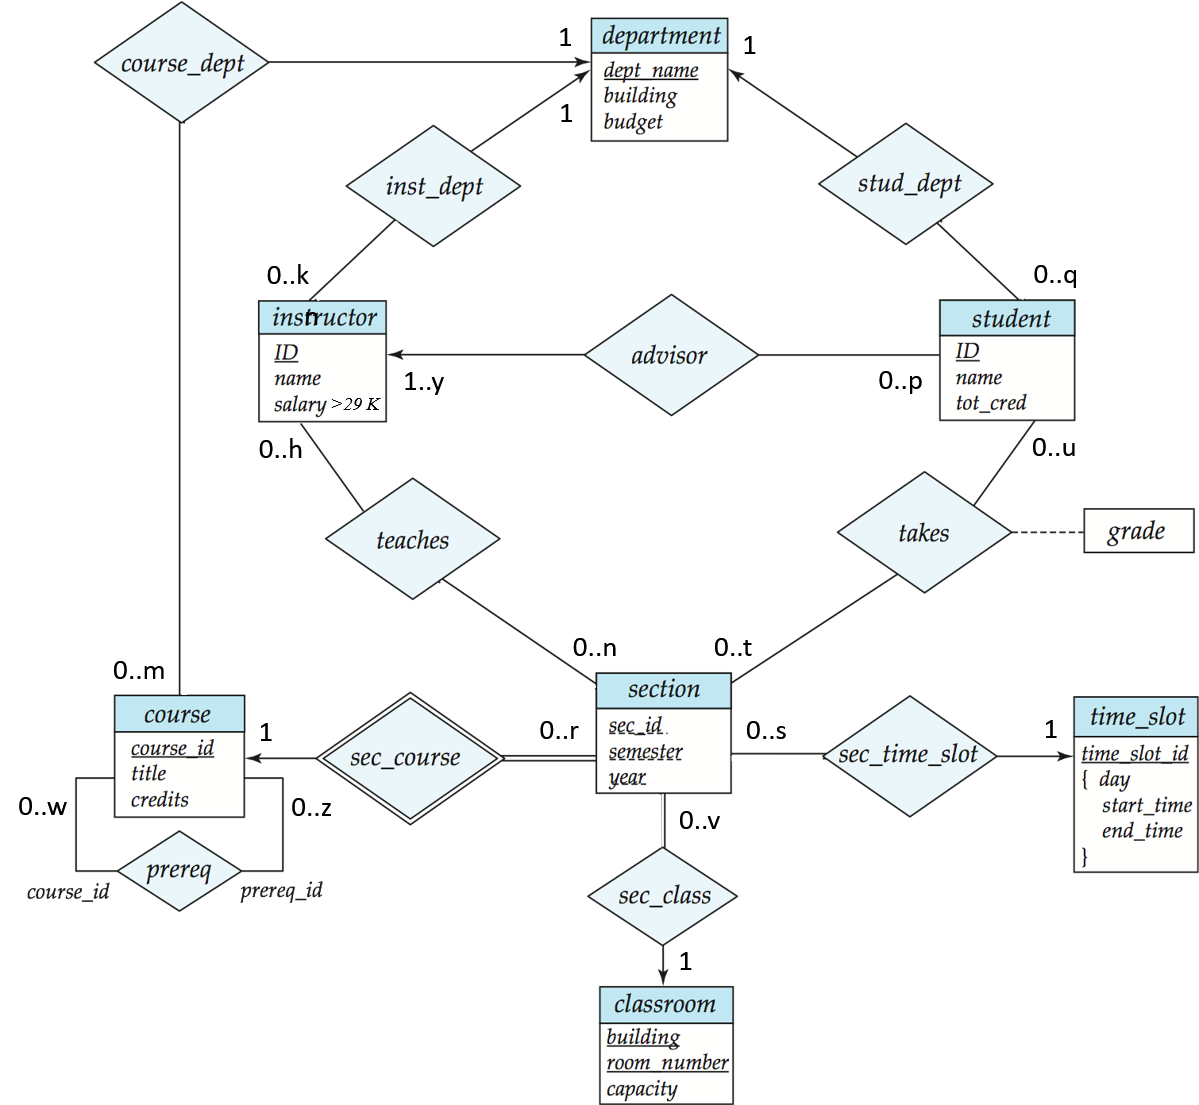
\includegraphics[scale=0.35]{img/ERM-UniversityUseCase.png}
\end{figure}
\end{frame}

\begin{frame}[t]
\frametitle{Anwendungsf\"alle}
\framesubtitle{\insertsubsection}
\begin{alertblock}{Aufgabenstellung}
\begin{enumerate}
	\item Erstellen Sie aus dem ER-Modell das logische Datenmodell 
	\item Implementieren Sie das logische Datenmodell auf der PostgreSQL-Datenbank 
	\item Befüllen Sie die Datenbank mit ausreichend vielen Testdaten aus dem Datenpool der Vorlesung
\end{enumerate}
\end{alertblock}
\abs
\abs
\textbf{Beachten Sie:} Das ER-Modell soll in seiner \"au\ss eren Struktur -- Entit\"aten, Beziehungen, Kardinalit\"aten -- realisiert 
werden. Die innere Struktur wie beispielsweise Anzahl, Art und Datentypen der Attribute k\"onnen Sie nach Ihren eigenen Ideen und
Vorstellungen entwerfen.
\end{frame}

\begin{frame}[t]
\frametitle{Anwendungsf\"alle}
\framesubtitle{\insertsubsection}
\begin{alertblock}{Aufgabenstellung (Fortsetzung)}
\begin{enumerate}
 \setcounter{enumi}{3}	
 % 2.2
 \item Betrachten Sie die Fremdschl\"usselbeziehung vom \texttt{dept\_name}-Attribute von der Relation der Dozenten 
  (\texttt{instructor}) auf die Fakult\"aten-Relation (\texttt{department}). Geben Sie Beispiele von Eingabe- 
  und L\"oschoperationen auf diesen Tabellen an, die eine Verletzung der Fremdschl\"usselbeziehung zur Folge haben.
 % 2.5
 \item\label{first} Was ist das Ergebnis der Hintereinanderausf\"uhrung folgender Operationen: 
  \begin{itemize} 
	 \item Kartesisches Produkt der Relationen \texttt{student} und \texttt{advisor} (und ggf.~\texttt{instructor}).
	 \item Selektion auf diesem Produkt mit der Bedingung \texttt{s\_id}$=$\texttt{i\_ID}? 
  \end{itemize}
  F\"uhren Sie die entsprechende SQL-Anweisung auf der Datenbank durch.
\end{enumerate}
\end{alertblock}
\end{frame}

\begin{frame}[t]
\frametitle{Anwendungsf\"alle}
\framesubtitle{\insertsubsection}
\begin{alertblock}{Aufgabenstellung (Fortsetzung)}
\begin{enumerate}
 \setcounter{enumi}{5}	
 % 2.6
 \item\label{U1} F\"uhren Sie folgende Operationen der relationalen Algebra in SQL auf der Datenbank aus.
  \"Uberlegen Sie sich vorab, welches Ergebnis die jeweilige Operation liefert.
  \begin{itemize}
   \item $\sigma_{year= 2009}(\texttt{section}\bowtie\texttt{takes})\bowtie\texttt{student}$
   \item $\sigma_{year= 2009}(\texttt{section}\bowtie\texttt{takes}\bowtie\texttt{student})$
   \item $\Pi_{ID,name,course\_id}(\texttt{section}\bowtie\texttt{takes}\bowtie\texttt{student})$
  \end{itemize}
 % 3.4
 \item\label{U2} F\"uhren Sie die folgenden Inserts, Updates, Deletes auf der Datenbank durch:
  \begin{itemize}
   \item Erh\"ohe das Gehalt jedes Dozenten in der Fakult\"at Informatik (\texttt{Comp. Sci.}) um 10\%.
   \item L\"osche alle Kurse, die nie angeboten wurden, d.~h., die nicht in der \texttt{section}-Tabelle vorkommen.
   \item F\"uge jede(n) Studierende(n) mit mehr als 100 Gesamt-Credit-Points (\texttt{tot\_cred}) in die 
    \texttt{instructor}-Tabelle mit einem Gehalt von 10.000 \$ ein. Vorsicht!
  \end{itemize}
\end{enumerate}
\end{alertblock}
\end{frame}

\begin{frame}[t]
\frametitle{Anwendungsf\"alle}
\framesubtitle{\insertsubsection}
\begin{alertblock}{Aufgabenstellung (Fortsetzung)}
\begin{enumerate}
 \setcounter{enumi}{7}	
 % 3.1 
 \item\label{U3} Dr\"ucken Sie die folgenden Anfragen in SQL aus und f\"uhren Sie die entsprechende Abfrage auf der 
  Datenbank durch:
  \begin{itemize}
   \item Finde die Kurse in der Fakult\"at Informatik (\texttt{Comp.~Sci.}) mit drei credit points.
   \item Finde die \texttt{ID}s aller Studenten, die Dozent (\texttt{instructor}) 
    \texttt{Bondi} unterrichtet. 
   \item Finde das h\"ochste Gehalt eines Dozenten. Finde alle Dozenten mit h\"ochstem Gehalt.
   \item Finde die Anzahl Einschreibungen in jeder Sektion (Tabelle \texttt{section}) eines Kurses im Wintersemester 
    (\texttt{Fall}) 2009.
   \item Finde die maximale Einschreibungszahl im Wintersemester (\texttt{Fall}) 2009.
   \item Finde die Sektionen mit maximaler Einschreibungszahl im Wintersemester (\texttt{Fall}) 2009.
  \end{itemize}
\end{enumerate}
\end{alertblock}
\end{frame}

\begin{frame}[t]
\frametitle{Anwendungsf\"alle}
\framesubtitle{\insertsubsection}
\begin{alertblock}{Aufgabenstellung (Fortsetzung)}
\begin{enumerate}
 \setcounter{enumi}{8}	
 % 4.1
 \item\label{U4} F\"uhren Sie folgende Anfragen auf der Datenbank aus: 
  \begin{itemize}
   \item Anzeige aller Dozenten mit ihren IDs, Namen und die Anzahl von Sektionen, die sie lehrten (Anzeige "0", falls 
    keine Sektion gelehrt wurde). 
   \item Anzeige aller Kombinationen von Sektionen, die im Sommersemester (\texttt{Spring}) 2010 angeboten wurden, 
    und den Namen der zugeh\"origen Dozenten. Wenn eine Sektion nicht gelehrt wurde, soll sie mit Dozentennamen 
    '\texttt{-}' ausgegeben werden.
   \item Anzeige aller Fakult\"aten (\texttt{department}) und der Gesamtzahl der zu der jeweiligen Fakult\"at
    geh\"orenden Dozenten. Auch Fakult\"aten ohne Dozenten sollen korrekt angezeigt werden.    	
  \end{itemize}
 % 4.2 
 \item\label{U5} Outer Joins k\"onnen in SQL ohne die explizite Verwendung der '\texttt{OUTER JOIN}'-Operation ausgef\"uhrt werden.
  Zeigen Sie das anhand der folgenden SQL-Anfragen:
  \begin{itemize}
   \item \texttt{SELECT * FROM student NATURAL LEFT OUTER JOIN takes}
   \item \texttt{SELECT * FROM student NATURAL FULL OUTER JOIN takes}
  \end{itemize}
\end{enumerate}
\end{alertblock}
\end{frame}

\begin{frame}[t]
\frametitle{Anwendungsf\"alle}
\framesubtitle{\insertsubsection}
\begin{alertblock}{Aufgabenstellung (Fortsetzung)}
\begin{enumerate}
 \setcounter{enumi}{10}	
 % 4.8
 \item\label{U6} Ein Dozent kann nicht zwei oder mehr Sektionen im gleichen time slot im Semester und Jahr unterrichten. 
  \begin{itemize}
   \item Schreiben Sie eine SQL-Abfrage, mit der alle (Dozent,Sektion)-Tupel bestimmt werden, die diese Bedingung verletzen
   \item \"Uberlegen Sie sich, wie diese Bedingung bereits in den Relationenschemata und den Integrit\"atsbedingungen
    festgelegt werden kann, um falsche Dateneingaben zu vermeiden.
  \end{itemize}
\end{enumerate}
\end{alertblock}
\end{frame}


% ANWENDUNGSPROGRAMMIERUNG
% Basic
%!TEX root = Slides.tex
\part{Grundlagen der Datenbankprogrammierung}
\label{part:programmierung}

\section{Systemarchitekturen}
\subsection{Grundlegendes}

\begin{frame}[t]
\frametitle{\insertsection}
\framesubtitle{\insertsubsection}
\structure{Benutzer und Anwendungen wollen auf Daten einer Datenbank zugreifen}\\[4pt]
\begin{itemize}
 \item Abfragedetails bzw. Abfragesprachen wie SQL sollen nach Möglichkeit vor Anwender verborgen bleiben
 \item Datenhaltung soll austauschbar sein -- Umzug auf anderes (R)DBMS soll minimale bis keine Auswirkungen auf Anwendung haben
 \item (R)DBMS soll zentrale Schnittstelle f\"ur Datenzugriff bilden
\end{itemize}
\abs
Im Laufe der Zeit haben sich mehrere Architekturmodelle gebildet.
\end{frame}

\begin{frame}[t]
\frametitle{\insertsection}
\framesubtitle{\insertsubsection}	
\structure{2-Schichten-Architekturen (2-Tier Architectures)}
\begin{figure}
	\begin{tikzpicture}[
 		block/.style={draw, fill=white,	rectangle, minimum width={width("Magnetometer2222")+2pt},	font=\small}]
			\node[block, fill=blue!30, align=center] (tier1) {Präsentations-\\Schicht};
 			\node[block, fill=blue!30, align=center] (tier2) [below=0mm of tier1] {Anwendungs-\\logik};
 			\node[block, fill=red!30, align=center] (tier3) [below=4mm of tier2] {Datenhaltung}; 
 			\draw (tier2) -- (tier3);				
 			\node[block,fill=blue!30, align=center] (tier21) [left=30mm of tier1] {Präsentations-\\Schicht};
 			\node[block,fill=red!30, align=center] (tier22) [below=4mm of tier21] {Anwendungs-\\logik};
 			\node[block,fill=red!30, align=center] (tier23) [below=0mm of tier22] {Datenhaltung}; 
 			\draw (tier21) -- (tier22);
	\end{tikzpicture}
	\caption{\label{fig:2tier}Zwei alternative 2-Schichten-Architekturen}
\end{figure}		
\end{frame}

\begin{frame}[t]
\frametitle{\insertsection}
\framesubtitle{\insertsubsection}		
\onslide
\structure{Eigenschaften klassischer 2-Schichten-Architekturen}\\[4pt]
	\begin{itemize}
		\item Programmiersprachen: häufig 4GL-Sprachen 
		% Fourth generation language oder kurz 4GL: 
		% Programmiersprachen bzw. -umgebungen, die darauf ausgerichtet sind, rasch – mit möglichst wenigen Codezeilen – 
		% für bestimmten Anwendungsbereich Funktionen oder komplette Anwendungen schreiben zu können und
		% Integration von Datenbank- und Benutzerschnittstellenanweisungen in die Programmiersprache
		%    Befehle zur Abfrage und Manipulation einer Datenbank
		%    Befehle zur einfachen Erstellung von Benutzeroberflächen
		% 4GL-Programmiersprachen: Java, C++, auch SQL
		\begin{itemize}
			\item Speziell für die Entwicklung datenzentrischer Anwendungen
			\item Meist automatische Erstellung von Benutzeroberflächen auf Basis des Datenmodells 
		  \item Leichte und schnelle Entwicklung
		\end{itemize}
		\pause
		\item Nachteile
		\begin{itemize}
			\item Starke Kopplung zwischen den einzelnen Schichten 
			\item Keine Komponente kann ersetzt werden, ohne die anderen Komponenten anpassen zu m\"ussen
			\item Große Systeme werden schnell un\"ubersichtlich 
		\end{itemize}
	\end{itemize}
\pause
\abs
\structure{Durch die schwierige Wartbarkeit und mangelnde Flexibilität sind klassische 2-Schichten-Architekturen 
	heute eher die Ausnahme.}\\[4pt]
\pause
\structure{Moderne 2-Schichten-Architekturen haben Eigenschaften von 3-Schichten-Architekturen
	mit API-separierter Anwendungslogik und Datenhaltung in unterer Schicht}				
\end{frame}

\begin{frame}[t]
\frametitle{\insertsection}
\framesubtitle{\insertsubsection}
\structure{3-Schichten-Architekturen}\\[8pt]
\begin{figure}
	\centering
	\begin{tikzpicture}[block/.style={draw,	fill=white,	rectangle, minimum width={width("Magnetometer2222")+2pt},	font=\small}]
 	\node[block, fill=blue!30, align=center] (tier1) {Client Tier};
	\node[block, fill=green!30, align=center] (tier2) [below=4mm of tier1] {Middle Tier};
	\node[block, fill=red!30, align=center] (tier3) [below=4mm of tier2] {Server Tier}; 
	\draw (tier1) -- (tier2); 
	\draw (tier2) -- (tier3);
	\end{tikzpicture}
	\qquad	
	\begin{tikzpicture}[block/.style={draw,	fill=white,	rectangle, minimum width={width("Magnetometer2222")+2pt},	font=\small}]
	\node[align=center] (tier1f) {};
	\node[align=center] (tier2f) [below=4mm of tier1f] {$\Longrightarrow$};
	\node[align=center] (tier3f) [below=4mm of tier2f] {}; 
	\draw (tier1f) -- (tier2f); 
	\draw (tier2f) -- (tier3f);
	\end{tikzpicture}
	\qquad
	\begin{tikzpicture}[block/.style={draw,	fill=white,	rectangle, minimum width={width("Magnetometer2222")+2pt},	font=\small}]
	\node[block, fill=blue!30, align=center] (tier1c) {Pr\"asentation};
	\node[block, fill=green!30, align=center] (tier2c) [below=4mm of tier1c] {Anwendung};
	\node[block, fill=red!30, align=center] (tier3c) [below=4mm of tier2c] {Datenhaltung}; 
	\draw (tier1c) -- (tier2c); 
	\draw (tier2c) -- (tier3c);
	\end{tikzpicture}
	\caption{\label{fig:3tier}3-Schichten-Architektur}
\end{figure}		
\end{frame}

\begin{frame}[t]
\frametitle{\insertsection}
\framesubtitle{\insertsubsection}
\onslide
\structure{Eigenschaften von 3-Schichten-Architekturen}\\[4pt]
\begin{itemize}
	\item Client-Schicht ausschließlich für Pr\"asentation der Ergebnisse und Daten 
	\item Anwendungslogik befindet sich in mittlerer Schicht 
	\begin{itemize}
		\item Berechnungsvorschriften
		\item Abläufe
		\item $\dots$
	\end{itemize}
	\item Datenhaltung in Server-Schicht kein Bestandteil der Anwendungslogik 
	\begin{itemize}
		\item Einheitliche Zugriffskonzepte und Schnittstellen
	\end{itemize}
\end{itemize}
\pause
\abs
\structure{Durch klare Schnittstellen/Zust\"andigkeiten k\"onnen die einzelnen Schichten modifiziert werden, 
	ohne zu starte Einfl\"usse auf benachbarte Schichten bef\"urchten zu m\"ussen.}
\\[4pt]
\pause
\structure{Zur Erinnerung: Moderne 2-Schichten-Architekturen haben Eigenschaften von 3-Schichten-Architekturen
	mit API-separierter Anwendungslogik und Datenhaltung}				
\end{frame}

\subsection{Zugriff auf Datenbanken}
\begin{frame}[t]
\frametitle{\insertsection}
\framesubtitle{\insertsubsection}
\onslide
\structure{Zugriffskonzepte und Schnittstellen f\"ur programmatischen Zugriff auf Datenbanken}\\[4pt]
\begin{description}[leftmargin=0cm]
	\item[ODBC] Open Database Connectivity. Klassische Schnittstelle für Zugriffe auf RDBMS
	\item[OLEDB] Designierter Nachfolger von ODBC, jedoch komplexer
	\item[DAO] Data Access Objects. In erster Linie von Microsoft entwickelt, kann auch auf ODBC-Quellen zugreifen
	\item[ADO] ActiveX Data Objects. Zugriff auf tabellenartige Datenquellen (RDBMS, CSV etc.)
	\item[ADO.NET] Reimplementierung von ADO auf~.NET-Framework von Microsoft
	\item[JDBC] Java Database Connectivity. F\"ur Java-Programmierung, vergleichbar mit ODBC 
\end{description}
\pause
\abs
\structure{In Vorlesung: JDBC}
\end{frame}

\section{JDBC}
\subsection{Einführung}

\begin{frame}[t]
\frametitle{\insertsection}
\framesubtitle{\insertsubsection}
\onslide
\begin{itemize}
	\item Zuerst von Sun Microsystems (jetzt Oracle) entwickelt
	\item DBMS-neutrale Schnittstelle (API) f\"ur Datenbankzugriffe
	\item Direkte Nutzung von SQL-Statements[4pt]
%	\pause
%	\item Liegt in verschiedenen Versionen vor:
%	\begin{itemize}
%		\item JDBC V1 konnte herstellerunabhängige Verbindungen zu Datenbanken aufbauen und einfache Queries verarbeiten
%		\item JDBC V2 konnte änderbare Ergebnismengen verarbeiten, außerdem kannte es neue Datentypen und Connection Pooling
%		\item JDBC V3 wurde mit weiteren Änderungsmethoden sowie benutzerdefinierten Datentypen erweitert
%		\item JDBC V4 ist in erster Linie ein Performance-Update 
%	\end{itemize}
\end{itemize}
\end{frame}

\begin{frame}[t]
\frametitle{\insertsection}
\framesubtitle{\insertsubsection}
\structure{Idee von JDBC}\\[4pt]
\begin{columns}[c]
	\begin{column}{.35\textwidth}
		\begin{figure}
			\begin{tikzpicture}[block/.style={draw,	fill=white,	rectangle, minimum width={width("Magnetometer2222")+2pt},	font=\small}]
			\node[block, fill=blue!30, align=center] (tier1) {Java\\Application};
			\node[block, fill=blue!20, align=center] (tier2) [below=0mm of tier1] {JDBC -- API};
			\node[block, fill=orange!60, align=center] (tier2b) [below=0mm of tier2] {JDBC -- Impl.};
			\node[drop shadow, fill=orange, cylinder,minimum height=0.5cm, draw, shape border rotate=90, minimum width=2cm] 
			(db) [below=5mm of tier2b] {DB};
			\draw (tier2b) -- (db);
			\end{tikzpicture}
			\caption{\label{fig:jdbc}JDBC-Konzept}
		\end{figure}		
	\end{column}
	\begin{column}{.65\textwidth}
		\begin{itemize}
			\item JDBC-API befindet sich im Package \texttt{java.sql}
			\item Java-Applikation und JDBC in Anwendungsschicht
			\item Kommunikation mit Datenbanken durch (propriet\"are) \textbf{JDBC-Treiber}, die JDBC-API implementieren.
		\end{itemize}
	\end{column}
\end{columns}
\end{frame}

%%%%%%%%%%%%%%%%%%%%%%%%%%%%%%%%
% wird voererst weggelassen
%%%%%%%%%%%%%%%%%%%%%%%%%%%%%%%%
\nowrite{ 
\begin{frame}[t]
\frametitle{\insertsection}
\framesubtitle{\insertsubsection}
\begin{columns}
	\begin{column}{.48\textwidth}
		\begin{figure}
		 \pgfuseimage{jdbctypes}
		 \tiny Bildquelle: Wikipedia
		 \caption{JDBC Treibertypen}
		\end{figure}		
	\end{column}
	\begin{column}{.48\textwidth}
		\begin{itemize}
			\item Typ-1-Treiber sind Bridge-Treiber zwischen Schnittstellentechnologien
			\item Typ-2-Treiber arbeiten direkt proprietären Bibliotheken 
			\item Typ-3-Treiber nutzen einen Middleware-Server
			\item Typ-4-Treiber kommunizieren direkt mit der DB 
		\end{itemize}
		Die meisten JDBC-Treiber sind Typ-4-Treiber.
	\end{column}
\end{columns}
\end{frame}
}
%%%%%%%%%%%%%%%%%%%%%%%%%%%%%%%%

\subsection{API -- Erste Schritte}

\begin{frame}[t]\frametitle{\insertsection}
\framesubtitle{\insertsubsection}
\structure{Die wichtigsten Objekte der JDBC-API}
\begin{figure}\scalebox{0.9}{
		\begin{tikzpicture}[
		block/.style={draw,	fill=white,	rectangle, minimum width={width("Magnetometer2222")+2pt},	font=\small}]
		\node[block, fill=blue!50, align=center] (rs) {ResultSet};
		\node[block, fill=blue!50, align=center] (st) [below=10mm of rs] {Statement};
		\node[block, fill=blue!50, align=center] (rs2) [right=40mm of rs] {ResultSet};
		\node[block, fill=blue!50, align=center] (pst) [below=10mm of rs2] {PreparedStatement};
		\node[block, fill=blue!50, align=center] (con) [below right=5mm of st] {Connection};
		\node[block, fill=blue!50, align=center] (dm) [below=10mm of con] {DriverManager};
		\draw (rs) -- (st); 
		\draw (rs2) -- (pst); 
		\draw (pst) -- (con);
		\draw (st) -- (con); 
		\draw (con) -- (dm);
		\end{tikzpicture}
	}
	\caption{\label{fig:APIStruktur}JDBC API-Struktur}
\end{figure}					
\vskip -1.2em
\structure{Doku: \href{https://docs.oracle.com/javase/9/docs/api/java/sql/package-summary.html}
	{\textcolor{blue}{\underline{Java API Specification Package \texttt{java.sql}}}}}
\end{frame}

\begin{frame}[fragile]
\frametitle{\insertsection}
\framesubtitle{\insertsubsection}
\onslide
\structure{\texttt{\textbf{DriverManager}} verwaltet die installierten und geladenen JDBC-Treiber}\\[8pt]
\begin{columns}
	\begin{column}{.3\textwidth}
		\begin{figure}\scalebox{.45}{
				\begin{tikzpicture}[block/.style={draw,	fill=white,	rectangle, minimum width={width("Magnetometer2222")+2pt},	font=\small}]
				\node[block, fill=blue!10, align=center] (rs) {ResultSet};
				\node[block, fill=blue!10, align=center] (st) [below=10mm of rs] {Statement};
				\node[block, fill=blue!10, align=center] (rs2) [right=40mm of rs] {ResultSet};
				\node[block, fill=blue!10, align=center] (pst) [below=10mm of rs2] {PreparedStatement};
				\node[block, fill=blue!10, align=center] (con) [below right=5mm of st] {Connection};
				\node[block, fill=blue!50, align=center] (dm) [below=10mm of con] {DriverManager};
				\draw (rs) -- (st); 
				\draw (rs2) -- (pst); 
				\draw (pst) -- (con);
				\draw (st) -- (con); 
				\draw (con) -- (dm);
				\end{tikzpicture}
			}				
		\end{figure}
	\end{column}
	\begin{column}{.65\textwidth}
		\pause
		Treiber in System/Applikation vorab bekannt machen:
		\begin{enumerate}
			\item JDBC-Treiberpaket (\texttt{jar}) als Teil des \texttt{CLASSPATH} 
			\pause
			\item JDBC-API in Applikation: \texttt{import java.sql.*} 
			\pause
			\item Laden des propriet\"aren JDBC-Treibers (alternativ):
			\begin{itemize}
				\item In Applikation: \texttt{Class.forName("{org}.postgresql.Driver");}
				\item Bei Ausf\"uhrung: \texttt{java~-Djdbc.drivers=org.postgresql.Driver MyApp}
			\end{itemize} 
		\end{enumerate}
		%\lstset{language=Java}
		%\lstset{escapeinside={(*@}{@*)}}
		%\begin{lstlisting}[xleftmargin=3ex,numbers=none]
		%try {
		%Class.forName("com.mysql.jdbc.Driver").newInstance(); (*@\label{lst:classforname}@*)
		%} catch (Exception e) {
		%...
		%}
		%\end{lstlisting}
		%Zeile \ref{lst:classforname} lädt den Treiber unter dem angegebenen Namen, so dass er von der JVM verwendet werden kann.
	\end{column}
\end{columns}
\end{frame}

\begin{frame}[fragile]
\frametitle{\insertsection}
\framesubtitle{\insertsubsection}
\structure{\texttt{\textbf{Connection}}-Objekt repräsentiert Verbindung zur Datenbank}\\[8pt]
\begin{columns}
	\begin{column}{.3\textwidth}
		\begin{figure}\scalebox{.45}{
				\begin{tikzpicture}[block/.style={draw,	fill=white,	rectangle, minimum width={width("Magnetometer2222")+2pt},	font=\small}]
				\node[block, fill=blue!10, align=center] (rs) {ResultSet};
				\node[block, fill=blue!10, align=center] (st) [below=10mm of rs] {Statement};
				\node[block, fill=blue!10, align=center] (rs2) [right=40mm of rs] {ResultSet};
				\node[block, fill=blue!10, align=center] (pst) [below=10mm of rs2] {PreparedStatement};
				\node[block, fill=blue!50, align=center] (con) [below right=5mm of st] {Connection};
				\node[block, fill=blue!10, align=center] (dm) [below=10mm of con] {DriverManager};
				\draw (rs) -- (st); 
				\draw (rs2) -- (pst); 
				\draw (pst) -- (con);
				\draw (st) -- (con); 
				\draw (con) -- (dm);
				\end{tikzpicture}
			}				
		\end{figure}
	\end{column}
	\begin{column}{.65\textwidth}
		Von \texttt{DriverManager} mit Hilfe einer \textit{connection URL} erzeugt:
\lstset{language=Java}
\lstset{escapeinside={(*@}{@*)}}
\begin{lstlisting}[xleftmargin=3ex, numbers=none]
 ...
 String url = "jdbc:postgresql://<host><:port></database>";
 Connection conn = DriverManager.getConnection(url,uname,pwd);
 ...
\end{lstlisting}
	\end{column}
\end{columns}
\end{frame}

\begin{frame}[fragile]
\frametitle{\insertsection}
\framesubtitle{\insertsubsection}
\structure{\texttt{\textbf{Statement}}}\\[8pt]
\begin{columns}
	\begin{column}{.3\textwidth}
		\begin{figure}\scalebox{.45}{
				\begin{tikzpicture}[block/.style={draw,	fill=white,	rectangle, minimum width={width("Magnetometer2222")+2pt},	font=\small}]
				\node[block, fill=blue!10, align=center] (rs) {ResultSet};
				\node[block, fill=blue!50, align=center] (st) [below=10mm of rs] {Statement};
				\node[block, fill=blue!10, align=center] (rs2) [right=40mm of rs] {ResultSet};
				\node[block, fill=blue!10, align=center] (pst) [below=10mm of rs2] {PreparedStatement};
				\node[block, fill=blue!10, align=center] (con) [below right=5mm of st] {Connection};
				\node[block, fill=blue!10, align=center] (dm) [below=10mm of con] {DriverManager};
				\draw (rs) -- (st); 
				\draw (rs2) -- (pst); 
				\draw (pst) -- (con);
				\draw (st) -- (con); 
				\draw (con) -- (dm);
				\end{tikzpicture}
			}				
		\end{figure}
	\end{column}
	\begin{column}{.65\textwidth}
		\begin{itemize}
			\item \texttt{Statement} repr\"asentiert einen SQL-Befehl
			\item Mit \texttt{Connection}-Objekt erzeugt:
		\end{itemize}
\lstset{language=Java}
\lstset{escapeinside={(*@}{@*)}}
\begin{lstlisting}[numbers=none]
...
Statement stmt = conn.createStatement(); 
...
\end{lstlisting}
	 \begin{itemize}
	  \item Ausf\"uhrung des \texttt{Statement}-Objekts f\"uhrt zur Rückgabe eines \texttt{ResultSet} ...
   \end{itemize}
	\end{column}
\end{columns}
\end{frame}

\begin{frame}[fragile]
\frametitle{\insertsection}
\framesubtitle{\insertsubsection}
\structure{\texttt{\textbf{ResultSet}}}\\[8pt]
\begin{columns}
	\begin{column}{.3\textwidth}
		\begin{figure}\scalebox{.45}{
				\begin{tikzpicture}[block/.style={draw,	fill=white,	rectangle, minimum width={width("Magnetometer2222")+2pt},	font=\small}]
				\node[block, fill=blue!50, align=center] (rs) {ResultSet};
				\node[block, fill=blue!10, align=center] (st) [below=10mm of rs] {Statement};
				\node[block, fill=blue!10, align=center] (rs2) [right=40mm of rs] {ResultSet};
				\node[block, fill=blue!10, align=center] (pst) [below=10mm of rs2] {PreparedStatement};
				\node[block, fill=blue!10, align=center] (con) [below right=5mm of st] {Connection};
				\node[block, fill=blue!10, align=center] (dm) [below=10mm of con] {DriverManager};
				\draw (rs) -- (st); 
				\draw (rs2) -- (pst); 
				\draw (pst) -- (con);
				\draw (st) -- (con); 
				\draw (con) -- (dm);
				\end{tikzpicture}
			}				
		\end{figure}
	\end{column}
	\begin{column}{.65\textwidth}
		\begin{itemize}
			\item \texttt{ResultSet} als Ergebnis der Ausf\"uhrung eines \texttt{Statement}-Objekts
			\item \texttt{ResultSet} repr\"asentiert und beinhaltet die Ergebnismenge (Tupeln) eines SQL-Befehls
		\end{itemize}
	\end{column}
\end{columns}
\end{frame}

\begin{frame}[t]
\frametitle{\insertsection}
\framesubtitle{\insertsubsection}
\onslide
\structure{\texttt{\textbf{ResultSet}} und \texttt{\textbf{Statement}}}\\[8pt]
\structure{Unterschiedliche Ausf\"uhrungsmethoden:}
\begin{itemize}
	\item \texttt{Statement.execute(String sql)}
	\begin{itemize}
		\item F\"uhrt SQL-Befehl \texttt{sql} auf Datenbank aus
		\item Rückgabe: \texttt{true}, wenn Ausf\"uhrung erfolgreich, sonst \texttt{false}
		\item Resultate danach mit Methode \texttt{getResultSet()} abrufen. R\"uckgabe: \texttt{ResultSet}
	\end{itemize}
	\pause 
	\item \texttt{Statement.executeQuery(String sql)}
	\begin{itemize}
		\item F\"uhrt SQL-Befehl \texttt{sql} aus 
		\item R\"uckgabe: \texttt{ResultSet} 
		\item \texttt{ResultSet} ist \texttt{null} im Fehlerfall
	\end{itemize}
	\pause 
	\item \texttt{Statement.executeUpdate(String sql)}
	\begin{itemize}
		\item F\"uhrt SQL-Befehl \texttt{sql} aus
		\item R\"uckgabe: Anzahl (\texttt{int}) der vom Update betroffenen Tupel
	\end{itemize}
\end{itemize}
\end{frame}

\begin{frame}[fragile]
\frametitle{\insertsection}
\framesubtitle{\insertsubsection}
\structure{\texttt{\textbf{ResultSet}} -- Beispiel}\\[4pt]
\lstset{language=Java}
\lstset{escapeinside={(*@}{@*)}}
\begin{lstlisting}[xleftmargin=3ex, numbers=none, showstringspaces=false]
...
Statement stmt = conn.createStatement(); 
String sql = "SELECT * FROM \"MySchema\".\"Film\"";

if(stmt.execute(sql)){
 ResultSet rs = stmt.getResultSet(); 
 // Resultat mit ResultSet rs verarbeiten - naechste Folie
} 
\end{lstlisting}
\end{frame}

\begin{frame}[fragile]
\frametitle{\insertsection}
\framesubtitle{\insertsubsection}
\onslide
\structure{\texttt{\textbf{ResultSet}}}\\[4pt]
\begin{itemize}
	\item \texttt{ResultSet} weist intern eine tabellarische Struktur auf und kann daher \"ahnlich wie eine Relation gesehen werden
	\pause
	\item F\"ur das Traversieren eines \texttt{ResultSet} werden entsprechende Methoden bereitgestellt
	\begin{itemize}
		\item \texttt{next()} setzt den Zugriffs-Pointer auf den nächsten Eintrag und gibt \texttt{false} zur\"uck, wenn es kein 
		weiteres Tupel gibt 
		\item Nur f\"ur \texttt{scrollable ResultSet}:
		\begin{itemize}
			\item \texttt{previous()} setzt Zugriffs-Pointer vorherigen Eintrag
			\item \texttt{first()} setzt den Zugriffs-Pointer \textbf{auf} den ersten Eintrag
			\item \texttt{last()} setzt Zugriffs-Pointer auf letzten Eintrag
			\item \texttt{beforeFirst()} setzt Zugriffs-Pointer \textbf{vor} den ersten Eintrag
			\item \texttt{afterLast()} setzt Zugriffs-Pointer \textbf{nach} letzten Eintrag
		\end{itemize}
	\end{itemize}
	\item Traversieren eines \texttt{ResultSet} meist mit Hilfe einer Schleife -- n\"achste Folie
	\pause
	\item Typisierter Zugriff auf Daten eines Tupels des \texttt{ResultSet}:
	\begin{itemize}
		\item Zugriff über Spaltenindex bzw.~Spaltenname m\"oglich: z.B. \texttt{getInt(3)}, \texttt{getInt("Jahr")},
		\texttt{getString("Name")}
	\end{itemize}
\end{itemize}
\end{frame}

\begin{frame}[fragile]
\frametitle{\insertsection}
\framesubtitle{\insertsubsection}
\structure{\texttt{\textbf{ResultSet}} -- Beispiel}
\lstset{language=Java}
\lstset{escapeinside={(*@}{@*)}}
\begin{lstlisting}[xleftmargin=3ex, showstringspaces=false, numbers=none]
...			
ResultSet rs = stmt.getResultSet(); 

//Durchlaufen des ResultSet
while (rs.next()) {
 System.out.println("Name des Films: " + rs.getString(2)); 
}
...
\end{lstlisting}
\end{frame}

\begin{frame}[fragile]\frametitle{\insertsection}
\framesubtitle{\insertsubsection}
\structure{\texttt{\textbf{ResultSet}} -- Metadaten}\\[4pt]
\begin{itemize}
\item \texttt{ResultSet} enthält Metadaten (Attributnamen, Datentypdefinitionen etc.).
\item Diese Informationen können mit einem Objekt vom Typ \texttt{ResultSetMetaData} abgerufen werden.
\end{itemize}
Beispiel:
\lstset{language=Java}
\lstset{escapeinside={(*@}{@*)}}
\begin{lstlisting}[xleftmargin=3ex, numbers=none]
...
ResultSet rs = stmt.getResultSet(); 
ResultSetMetaData rsmd = rs.getMetaData(); 

for (int i = 1; i <= rsmd.getColumnCount(); i++){
 String spaltenname = rsmd.getColumnLabel(i);
 String spaltentyp = rsmd.getColumnTypeName(i);
}
\end{lstlisting}
\end{frame}

\begin{frame}[fragile]
\frametitle{\insertsection}
\framesubtitle{\insertsubsection}
\structure{\texttt{\textbf{PreparedStatement}}}\\[8pt]
\begin{columns}
	\begin{column}{.3\textwidth}
		\begin{figure}\scalebox{.45}{
				\begin{tikzpicture}[block/.style={draw,	fill=white,	rectangle, minimum width={width("Magnetometer2222")+2pt},	font=\small}]
				\node[block, fill=blue!10, align=center] (rs) {ResultSet};
				\node[block, fill=blue!10, align=center] (st) [below=10mm of rs] {Statement};
				\node[block, fill=blue!10, align=center] (rs2) [right=40mm of rs] {ResultSet};
				\node[block, fill=blue!50, align=center] (pst) [below=10mm of rs2] {PreparedStatement};
				\node[block, fill=blue!10, align=center] (con) [below right=5mm of st] {Connection};
				\node[block, fill=blue!10, align=center] (dm) [below=10mm of con] {DriverManager};
				\draw (rs) -- (st); 
				\draw (rs2) -- (pst); 
				\draw (pst) -- (con);
				\draw (st) -- (con); 
				\draw (con) -- (dm);
				\end{tikzpicture}
			}				
		\end{figure}
	\end{column}
	\begin{column}{.65\textwidth}
		\begin{itemize}
			\item H\"aufig wiederkehrende Statements können durch ein \texttt{PreparedStatement} vorbereitet werden. 
			\item DBMS nimmt \texttt{PreparedStatement} entgegen
			\begin{itemize}
				\item bereitet den optimierten Ausführungsplan intern vor
				\item verwendet den optimierten Ausführungsplan fortan (im Kontext einer \texttt{Connection})
			\end{itemize}
		\end{itemize}
	\end{column}
\end{columns}
\end{frame}

\begin{frame}[fragile]
\frametitle{\insertsection}
\framesubtitle{\insertsubsection}
\onslide
\structure{\texttt{\textbf{PreparedStatement}} -- Syntax}
\lstset{language=Java}
\lstset{escapeinside={(*@}{@*)}}
\begin{lstlisting}[xleftmargin=3ex, showstringspaces=false]
String sql = "SELECT * FROM \"Film\" WHERE \"Name\" = ? AND \"Jahr\" = ?";

// PreparedStatement in RDBMS im Kontext der Connection conn
PreparedStatement pst = conn.prepareStatement(sql); 

// Parameter fuer PreparedStatement setzen
pst.setString(1,'Tatort'); (*@\label{lst:pst}@*)
pst.setInt(2,2011); (*@\label{lst:pst2}@*)

// SQL mit PrepraredStatement ausfuehren
ResultSet rs = pst.executeQuery(); 
\end{lstlisting}
\pause
\begin{itemize}
	\item Im SQL-String \texttt{sql} werden \texttt{?} als Platzhalter f\"ur Parameter verwendet.
	\item Diese Platzhalter werden mit \texttt{set}-Methoden belegt.
	\begin{itemize}
		\item In Zeile \ref{lst:pst} wird der erste Parameter auf den Wert \texttt{'Tatort'} gesetzt. 
		\item In Zeile \ref{lst:pst2} wird der zweite Parameter auf den Wert \texttt{2011} gesetzt. 
	\end{itemize}
\end{itemize}
\end{frame}

%!TEX root = Slides.tex
\section{Anwendungsf\"alle -- Programmierung}

\begin{frame}[t]
\frametitle{\insertsection}
\structure{\textbf{Auftragsmanagement}}\\[4pt]
\structure{\textbf{Universit\"atsverwaltung}}\\[8pt]
\begin{itemize}
	\item Programmierung von Java-Applikationen f\"ur die (parametrisierbare) Abfrage
	\item Pr\"asentation der Ergebnisse durch die Teams
\end{itemize}
\end{frame}

\subsection*{Auftragsmanagement}

\begin{frame}[t]
\frametitle{\insertsection}
\framesubtitle{\insertsubsection}
\begin{itemize}
\item Implementieren Sie die Datenbankabfragen aus den Aufgaben \ref{A1} -- \ref{A8} des Auftragsmanagements in Java. 
\item Parametrisieren Sie die in Java implementierten Abfragen aus den Aufgaben \ref{A4}, \ref{A7}, \ref{A8}. 
\end{itemize}
\end{frame}

\subsection*{Universit\"atsverwaltung}

\begin{frame}[t]
\frametitle{\insertsection}
\framesubtitle{\insertsubsection}
\begin{itemize}
	\item Implementieren Sie die Datenbankabfragen aus den Aufgaben \ref{U1}, \ref{U2}, \ref{U3}, \ref{U4} der 
	Universit\"atsverwaltung in Java. 
	\item Parametrisieren Sie wenn m\"oglich die in Java implementierten Abfragen. 
	\end{itemize}
\end{frame}


% Advanced
%!TEX root = Slides.tex
\part{Fortgeschrittene Datenbankprogrammierung}
\label{part:programmierungAdvanced}

\section{JDBC}
\subsection{Connection Pooling}

\begin{frame}[t]\frametitle{\insertsection}
\framesubtitle{\insertsubsection}
\structure{Verbindungsauf- und -abbau ist Flaschenhals bei Datenbankprogrammierung}
\begin{itemize}
	\item Verbindungsaufbau kostet im Allgemeinen sehr viel Zeit 
	\item Auf einzelner Verbindung kann nicht parallel gearbeitet werden. Mehrere Threads müssen 
	eigene Verbindungsobjekte erzeugen.
\end{itemize}
\onslide\pause 
\begin{block}{Connection Pooling}
	\begin{itemize}
		\item Mehre Verbindungen werden beim Start der Anwendung aufgebaut und in Pool gehalten
		\item Verbindungen aus Pool können sofort verwendet werden
		\item Nicht mehr benötigte Verbindungen werden nicht abgebaut, sondern in Pool zurückgegeben 
		\item Parameter steuern Verhalten des Pools -- wie viele Verbindungen usw.
	\end{itemize}
\end{block}
\end{frame}

\begin{frame}[fragile]\frametitle{\insertsection}
\framesubtitle{\insertsubsection}
\structure{Connection Pooling muss nicht selbst implementiert werden}
\abs
Verwende Bibliotheken f\"ur JDBC-konformes Connection Pooling. 
\nl
Beispiel: Open Source Bibliothek C3PO.
\abs
\onslide\pause
\begin{itemize}
\item C3PO verf\"ugbar unter \url{http://sourceforge.net/projects/c3p0/}
\item Paket muss im \texttt{CLASSPATH} liegen und kann sofort verwendet werden
\item Verbindungen zu Datenbanken werden über eigene Datenquelle (Data Source) bereitgestellt
\end{itemize} 
\end{frame}

\begin{frame}[fragile]\frametitle{\insertsection}
\framesubtitle{\insertsubsection\ -- Code-Beispiel}
\begin{lstlisting}[xleftmargin=3ex, showstringspaces=false, language=Java]
//Erstellen einer Datenquelle
ComboPooledDataSource cpds = new ComboPooledDataSource(); 
cpds.setDriverClass("org.postgresql.Driver");
cpds.setJdbcUrl("jdbc:postgresql://<host><:port></database>");
cpds.setUser("db");
cpds.setPassword("db"); 
cpds.setMinPoolSize(5); 
cpds.setAcquireIncrement(5);
cpds.setMaxPoolSize(100); 

//Verwendung der Datenquelle
Connection con1 = cpds.getConnection();
Connection con2 = cpds.getConnection();
...
\end{lstlisting}
\end{frame}

\begin{frame}[fragile]\frametitle{\insertsection}
\framesubtitle{\insertsubsection\ -- Web App Server}
\structure{Die meisten Web Application Server verf"ugen über eigenes Connection Pooling mittels JNDI}
\vspace{3mm}
Beispiel Apache Tomcat: Deskriptor \texttt{server.xml} und Java-Code gegenübergestellt
\begin{columns}
  \begin{column}{.48\textwidth}
  	\lstset{language=xml}
		\lstset{escapeinside={(*@}{@*)}}
\begin{lstlisting}[xleftmargin=3ex, basicstyle=\ttfamily\tiny, showstringspaces=false]
<Context>
 <Resource name="jdbc/TestDB" 
  auth="Container" type="javax.sql.DataSource" 
  maxActive="100" 
  maxIdle="30" 
  maxWait="1000" 
  username="<user>" 
  password="<password>" 
  driverClassName="org.postgresql.Driver"
  url="jdbc:postgresql://<host><:port></database>"/> 
</Context>
\end{lstlisting}
	\end{column}
	\begin{column}{.48\textwidth}
\lstset{language=Java}
			\lstset{escapeinside={(*@}{@*)}}
\begin{lstlisting}[xleftmargin=3ex, basicstyle=\ttfamily\tiny, showstringspaces=false, language=Java]
//Initialisierung
Context initContext = new InitialContext(); 
Context envContext = 
  (Context)initContext.lookup("java:/comp/env");
DataSource ds = 
  (DataSource)envContext.lookup("jdbc/TestDB");
			
//Jetzt kann Verbindung angefordert werden
Connection conn = ds.getConnection(); 
\end{lstlisting}
  \end{column}
\end{columns}
Web App Server verwaltet eigenen Connection Pool und stellt ihn Java-Anwendungen zur Verf\"ugung
\end{frame}

\subsection{Entwicklung von Anwendungen mit Datenbankanbindung}

\begin{frame}
	\frametitle{\insertsection}
	\framesubtitle{\insertsubsection}
	\structure{Wie es \textbf{nicht} geht:}
	\begin{itemize}
		\item Datenbankverbindungen und -abfragen im Code verstreuen
		\item Immer wieder durch ResultSets iterieren und quasi tabellarisch arbeiten
	\end{itemize}
\abs
	\structure{Stattdessen:}
	\begin{itemize}
		\item Entwerfen einer geeigneten Softwarearchitektur
		\item Nutzung der M\"oglichkeiten der Objektorientierung
	\end{itemize}	
\end{frame}

\begin{frame}
	\frametitle{\insertsection}
	\framesubtitle{\insertsubsection}
	\onslide
	\structure{Systematischer Aufbau:}
	\begin{itemize}
		\item Entwurf von Containerklassen f\"ur die Entit\"aten und Relationenschemata
		\begin{itemize}
			\item Verwendung von getter- und setter-Methoden
		\end{itemize}
 	  \pause
		\item Entwurf einer Zugriffsschnittstelle, die auf Containerklassen zugreift
		\pause
		\item Implementierung der Zugriffsschnittstelle f\"ur die konkrete Datenbank
		\pause
		\item Zugriff auf die Daten im Code \textit{ausschließlich über Zugriffsschnittstelle}
		\begin{itemize}
			\item ... am besten mittels Generator- oder Factory-Klasse
		\end{itemize}
	\end{itemize}
\end{frame}

\begin{frame}[fragile]\frametitle{\insertsection}
	\framesubtitle{\insertsubsection\ -- Beispiel}
	Containerklasse f\"ur Relationenschema
	\nl
	\texttt{\small Auto(int ID, varchar Name, varchar Marke, int[3] Farbe, int Leistung)}:
\begin{lstlisting}[xleftmargin=3ex, language=Java]
public class Auto{
 private int id; 		
 private int[] farbe; 		
 private int power; 
 ...

 public Auto() {farbe = new int[3];}

 public void setID(int id) {this.id = id;}
 public int getID() {return this.id;}

 public void setFarbe(int[] farbe) {this.farbe = farbe;}
 public int[] getFarbe() {return this.farbe;}

 public void setLeistung(int leistung) {this.power = leistung;}
 public int getLeistung() {return this.power;}
 ...
}
\end{lstlisting}
\end{frame}

\begin{frame}[fragile]\frametitle{\insertsection}
	\framesubtitle{\insertsubsection\ -- Beispiel}
	\structure{Zugriffsinterface}
\begin{lstlisting}[xleftmargin=3ex, language=Java]
public interface IRepository{
  public Auto createAuto(); 
		
  public Auto[] lookupAutoByFarbe(char[] farbe); 
  		
  public Auto[] lookupAutoByLeisung(int leistung); 

  public Auto lookupAutoById(int id); 
		
  public void saveAuto(Auto a); 	
}
\end{lstlisting}
\end{frame}

\begin{frame}[fragile]\frametitle{\insertsection}
	\framesubtitle{\insertsubsection\ -- Beispiel}
	\structure{Implementierungsklasse von Zugriffsinterface f\"ur PostgreSQL:}
\begin{lstlisting}[xleftmargin=3ex, showstringspaces=false, language=Java]
public class PostgreSQLRepository implements IRepository{
  private Connection con; 
  ... 
  
  public Auto lookupAutoById(int id){
    PreparedStatement pst = new PreparedStatement("SELECT * from Auto WHERE id = ?"); 
    pst.setInt(1,id); 
    ResultSet rs = pst.execute(); 
    Auto a = new Auto(); 
    
    while (rs.next()){
      a.setId(rs.getInt(0));
      a.setFarbe(rs.getFarbe(3));
      ...
    }
    return a;
  }
}
\end{lstlisting}
\end{frame}

\begin{frame}[fragile]\frametitle{\insertsection}
\framesubtitle{\insertsubsection\ -- Beispiel}
\structure{Factory-Klasse zur Erzeugung von Zugriffsinterfaces}
\begin{lstlisting}[xleftmargin=3ex, showstringspaces=false, language=Java]
public class RepoFactory{
  ...
  public static IRepository createRepository(ConfigObject config){
    if (config.getDatabase() == "Postgresql"){
      ...
      return new PostgreSQLRepository(); 
    } 
    else if (config.getDatabase() == "MySQL"){
      ...
      return new MySQLRepository(); 
    }
  }
}
\end{lstlisting}
Annahme: Config-Objekt \texttt{config} Konfigurationsdatei, in der die Datenbank konfiguriert wird.
\end{frame}

\begin{frame}[fragile]\frametitle{\insertsection}
\framesubtitle{\insertsubsection}
\structure{Zusammenfassung: Verwendung der Klassen}
\begin{lstlisting}[xleftmargin=3ex, showstringspaces=false, language=Java]
public static void main(String args[]){
  
  ConfigObject config = ...
  
  IRepository repo = RepoFactory.createRepository(config); 
  Auto auto = new Auto();
  auto.setLeistung(120);
  repo.saveAuto(auto)
  repo.lookupAutoByLeistung(120);
  
  Auto nocheinauto = new Auto(); 
  nocheinauto.setFarbe("schwarz");
  repo.saveAuto(nocheinauto);   
}
\end{lstlisting}
\end{frame}

\section{Objekt-relationales Mapping}
\subsection{Begriffserklärung}

\begin{frame}[t]\frametitle{Objekt-relationales Mapping}
    \framesubtitle{Begriffserklärung}
    \structure{Objektorientierte Welt: Objekte haben starke Strukturierung}
    \begin{itemize}
    	\item Schachtelung und komplexe Abhängigkeiten von Objekten
    	\item Vererbungshierarchien 
    	\item Schnittstellenkonzepte
    	\item Polymorphie und abstrakte Klassen
    \end{itemize}
\end{frame}

\begin{frame}[t]\frametitle{Objekt-relationales Mapping}
\framesubtitle{Begriffserklärung}
\structure{Relationale Welt:}
\begin{itemize}
	\item Tabellen sind "flach"
	\item Abhängigkeiten \"uber referentielle Integrit\"at 
	\item Keine inher\"anten Vererbungs-, Methoden- oder Schnittstellenkonzepte
\end{itemize}
\end{frame}

\begin{frame}[t]\frametitle{Objekt-relationales Mapping}
\framesubtitle{Begriffserklärung}
\onslide
\structure{Br\"ucke zwischen den Welten}
\begin{itemize}
	\item Versuch des Mapping zwischen objektorientierter und relationaler Welt 
	\item Mittels \textit{Object Flattening} werden strukturierte Objekte auf flache Tabellen und Schemata abgebildet
	\item Object Flattening erlaubt nur in gewissem Umfang die R\"uckabbildung von Schemata in Objekte
\end{itemize}
\pause
\begin{definition}[Object-Relational Impedance Mismatch]
	Unter dem Begriff \textit{Object-Relational Impedance Mismatch} wird die grundlegende Unverträglichkeit 
	von objektorientierten Programmiersprachen mit den Konzepten relationaler Datenbanken verstanden. 
	Es besteht ein \textit{Paradigmenkonflikt}.	
\end{definition}
\end{frame}

\againframe<2>{isa}

\begin{frame}[t]\frametitle{Objekt-relationales Mapping}
\framesubtitle{Ansätze für die Abbildung von is-a -- Beziehungen}
\structure{Es wurden verschiedene Möglichkeiten diskutiert:}
\onslide
\begin{itemize}
	\item One Table per Class Hierarchy 
	\begin{itemize}
		\item Attribute aller Entit\"aten der Klassenhierarchie in gemeinsames Relationenschema. 
		\item Unterscheidung der Entit\"aten durch Diskriminator-Attribut.
		\item \textbf{Problem:} Ansatz einfach zu implementieren, provoziert jedoch \texttt{null}-Werte und wird f\"ur 
		komplexere Hierarchien schwer wartbar.\\[4pt]
		%\item Normalisierung? 
	\end{itemize}
	\pause
	\item One Table per Concrete Class 
	\begin{itemize}
		\item Alle konkreten Klassen in eigenem Relationenschema.
		\item \textbf{Problem:} Informationen der Vererbung gehen verloren. Abstrakte Klasse existiert nicht mehr im Datenmodell.\\[4pt]
	\end{itemize}
	\pause
	\item One Table per Class
	\begin{itemize}
		\item Alle Klassen (auch die abstrakten) werden in eigenem Relationenschema abgebildet.
		\item \textbf{Problem:} Alle Vererbungsinformationen vorhanden, aber erhöhter Join-Aufwand 						
	\end{itemize}
\end{itemize}
\end{frame}

\begin{frame}[t]\frametitle{Objekt-relationales Mapping}
\framesubtitle{Verschiedene Konzepte}
\alert{Fazit: O-R-Mapping ist grundsätzliches Abbildungsproblem. Es gibt keine einheitliche Lösung.}
\abs
Entwickler arbeiten auf Objekten und m\"ussen Speicherung der Daten und Zerlegung der Objekte in Relationen manuell durchführen.
\abs
Dazu gibt es verschiedene Ansätze:
\onslide\pause
\begin{itemize}
	\item Objektorientierte Datenbanken 
	\begin{itemize}
		\item Objekte k\"onnen direkt in Datenbank abgelegt werden
		\item Nicht standardisiert. Auslesen der Objekte nur mit Hilfe der Anwendung möglich
		\item F\"ur spezielle Anwendungsfälle
	\end{itemize}
	\pause
	\item Erweiterung objektorientierter Programmiersprachen um relationale Konzepte
	\begin{itemize}
		\item SQL direkt im Code eingebettet
		\item Lösung widerspricht in großen Teilen objektorientierten Ansätzen
		\item Wird in der heutigen Entwicklung fast nicht mehr eingesetzt
	\end{itemize}
	\pause
	\item O/R-Mapper ...
\end{itemize}
\end{frame}

\subsection{O/R-Mapper}

\begin{frame}[t]\frametitle{Objekt-relationales Mapping}
	\framesubtitle{O/R-Mapper Allgemein}
	\structure{O/R-Mapper bilden eine Zwischenschicht zwischen Anwendung und Datenbank}
  \onslide
	\begin{itemize}
		\item Sie erledigen das Mapping von Objekten auf Relationen 
		\item Transparent für Anwendungsentwicklung
		\item Weite Verbreitung\\[8pt]
		\pause
		\item Viele unterschiedliche Implementierungen und Standards 
		\begin{itemize}
			\item Microsoft .NET Entity Framework 
			\begin{itemize}
				\item Alle .NET-Programmiersprachen (C\#, Visual Basic, Visual C++)
				\item Gute Unterstützung verschiedener Datenbanken
				\item Unterstützt Code-First und Model-First Ansätze
			\end{itemize}
			\item Java Persistence API (JPA)
			\begin{itemize}
				\item Standardisierte O/R-Mapper-Spezifikation für Java
			\end{itemize}
		\end{itemize}
	\end{itemize}
\end{frame}

\begin{frame}[t]\frametitle{Objekt-relationales Mapping}
	\framesubtitle{Java Persistence API (JPA)}
	\onslide
	\structure{Die JPA wurde erstmals 2006 veröffentlicht}
	\abs
	\begin{itemize}
		\item Standardisierte Programmierschnittstelle (API)
		\begin{itemize}
			\item Methoden zum Speichern, Modifizieren und Laden von Objekten aus relationalen Datenbanken
			\item Unterstützung von Polymorphie / Vererbung 
			\item Verwendet Java Annotations (z.B. \texttt{@Entity, @OneToMany})
		\end{itemize}
	\pause
		\item Java Persistence Query Language 
		\begin{itemize}
			\item Eigene, an SQL angelehnte Sprache
		\end{itemize}
		\item XML-Datei zur Konfiguration des relationalen Mappings
		\begin{itemize}
			\item Mittels \texttt{persistence.xml}-Datei kann das Mapping definiert werden
		\end{itemize}
	\pause
		\item Viele Implementierungen der JPA, z.B. \textit{Eclipselink} oder \textit{Hibernate}
	\end{itemize}
\end{frame}

\begin{frame}[t]\frametitle{Objekt-relationales Mapping}
	\framesubtitle{EclipseLink}
	\structure{JPA-Referenzimplementierung \textit{EclipseLink}}
	\abs
	\begin{itemize}
		\item Kann unter \url{https://www.eclipse.org/eclipselink/} heruntergeladen werden
		\item Umfasst mehr als nur eine JPA-Implementierung
		\item Konfiguration über \texttt{persistence.xml}
		\item Verwendung von Annotationen im Code
		\item Muss im \texttt{CLASSPATH} vorhanden sein
	\end{itemize}
\end{frame}

\begin{frame}[fragile]\frametitle{Objekt-relationales Mapping}
    \framesubtitle{Beispiel -- Tabellen f\"ur Genre und Film}
    \structure{persistence.xml}
\lstset{language=xml}
\lstset{escapeinside={(*@}{@*)}}
\begin{lstlisting}[xleftmargin=3ex, language=xml]
<?xml version="1.0" encoding="UTF-8" ?>
<persistence xmlns:xsi=...> 
 <persistence-unit name="filme" transaction-type="RESOURCE_LOCAL">   
  <class>de.test.Film</class>   
  <class>de.test.Genre</class>   
  <properties>     
   <property name="javax.persistence.jdbc.driver" value="org.postgresql.Driver"/>     
   <property name="javax.persistence.jdbc.url" 
             value="jdbc:postgresql://<host><:port></database>"/>
   <property name="javax.persistence.jdbc.user" value="<user>"/>
   <property name="javax.persistence.jdbc.password" value="<password>"/>
   <property name="eclipselink.ddl-generation" value="create-tables"/>
   <property name="eclipselink.ddl-generation.output-mode" value="database"/>
  </properties>
 </persistence-unit>
</persistence> 
	\end{lstlisting}
\end{frame}

\begin{frame}[fragile]\frametitle{Objekt-relationales Mapping}
    \framesubtitle{Beispiel -- Tabellen f\"ur Genre und Film}
    \structure{Java-Code \texttt{\small Film(FilmNr int,Name varchar(50),ErschJahr int,GenreID int)}}
\lstset{language=Java}
\lstset{escapeinside={(*@}{@*)}}
\begin{lstlisting}[xleftmargin=3ex, basicstyle=\ttfamily\tiny, language=Java]
package de.test;
import javax.persistence.*;

@Entity
public class Film{
 @Id
 @GeneratedValue(strategy=GenerationType.IDENTITY)
 @Column(name="FilmNr")
 private long filmid ; 

 @Column(name="Name")
 private String name ; 

 @Column(name="ErschJahr")
 private int jahr;

 @Column(name="GenreID")
 private int genreid;

 @OneToOne(cascade=CascadeType.PERSIST)
 @JoinColumn(name="GenreID")
 private Genre genre ; 

 //Getter und Setter fuer private Attribute
 ...
}
\end{lstlisting}
\end{frame}

% genauer im code:
% import javax.persistence.CascadeType;
% import javax.persistence.Entity;
% import javax.persistence.GeneratedValue;
% import javax.persistence.GenerationType;
% import javax.persistence.Id;
% import javax.persistence.OneToOne;

%\section*{Zusammenfassung}
%
%\begin{frame}{Zusammenfassung}
%	\begin{itemize}
%		\item Grundlagen über Systemarchitekturen
%		\begin{itemize}
%					\item 2-Tier
%					\item 3-Tier
%		\end{itemize}		
%		\item JDBC
%		\begin{itemize}
%			\item Einführung
%			\item API-Struktur
%			\item Connection Pooling
%		\end{itemize}
%		\item Object-relationaler Impedance Mismatch und O/R - Mapper
%	\end{itemize}
%
%\end{frame}
%

% ENTWURFSTHEORIE
% Relationale Entwurfstheorie - Kemper et al, Kapitel 6
%!TEX root = Slides.tex
\part{Entwurfstheorie}

\section{Problemstellung}

\begin{frame}\frametitle{\insertsection}
\begin{itemize}
	\item Bisher: Top-Down-Entwurf: Von der Anforderungsanalyse \"uber das ERM zum relationalen Schema
	\begin{itemize}
		\item Oft Datenredundanz, hohe Anzahl Attribute in Tabellen, etc. in Kauf genommen
		\item Oder zu viele schmale Relationen, Entit\"aten und Einheiten auseinandergebrochen, etc.
	\end{itemize}
  \pause
  \abs
	\item Besser: Konzeptuelle Feinabstimmung der erstellten relationalen Schemata
	\begin{itemize}
		\item Grundlage: Funktionale Abh\"angigkeiten und Schl\"ussel
		\item Ziel: G\"utebestimmung und Anpassung der Relationenschemata mit Hilfe von Normalformen und Normalisierungsalgorithmen
	\end{itemize}
	\end{itemize}
\end{frame}

\subsection{Breite Relationen}

\begin{frame}[t]\frametitle{\insertsection}
	\framesubtitle{\insertsubsection}
 	\structure{Gegeben sei die folgende recht breite Relation:}
 	\begin{center}
		\begin{tabular}{|c|c|c|c|c|c|}\hline
			\multicolumn{6}{|c|}{\small \textbf{Mitarbeiter\_Projekt}}\\\hline\hline
			 \small \textbf{\key{MANr}} & \small \textbf{Vorname}&\small \textbf{Nachname}&\textbf{\key{PNr}} &\small \textbf{Projektname}&\small \textbf{Funktion} \\\hline 
			\small 1 &\small Max & \small Mustermann &\small 4711 &\small Entwicklung &\small Entwickler \\\hline 
			\small 1 &\small Max & \small Mustermann &\small 4713 &\small Vertrieb & \small Kampagnen \\\hline 
			\small 2 &\small Erika &\small Musterfrau &\small 4711 &\small Entwicklung &\small SCRUM Master \\\hline 
			\small 2 &\small Erika &\small Musterfrau &\small 4712 &\small Test &\small Integrations-Tests \\\hline 
			\small 3 &\small Moritz & \small Musterherr &\small 4713 &\small Research &\small Leitung \\\hline 
		\end{tabular}
	\end{center}
	Relation hat einige problematische Eigenschaften, die zu \textit{Anomalien} führen können. 
\end{frame}

\begin{frame}[t]\frametitle{\insertsection}
\framesubtitle{\insertsubsection}
\structure{Redundanzproblem}
\begin{center}
	\begin{tabular}{|c|c|c|c|c|c|}\hline
		\multicolumn{6}{|c|}{\small \textbf{Mitarbeiter\_Projekt}}\\\hline\hline
		\small\textbf{\key{MANr}}&\small\textbf{Vorname}&\small\textbf{Nachname}&\textbf{\key{PNr}}&\small\textbf{Projektname}&\small\textbf{Funktion}\\\hline 
		\small 1 &\small Max & \small Mustermann &\small 4711 &\small Entwicklung &\small Entwickler \\\hline 
		\small \cellcolor{Red}1 &\small \cellcolor{Red}Max & \small \cellcolor{Red}Mustermann &\small 4713 
		&\small Vertrieb & \small Kampagnen \\\hline 
		\small 2 &\small Erika &\small Musterfrau &\small \cellcolor{Red}4711 &\small \cellcolor{Red}Entwicklung &\small SCRUM Master \\\hline 
		\small \cellcolor{Red}2 &\small \cellcolor{Red}Erika &\small \cellcolor{Red}Musterfrau 
		&\small 4712 &\small Test &\small Integrations-Tests \\\hline 
		\small 3 &\small Moritz & \small Musterherr &\small 4714 &\small Research &\small Leitung \\\hline 
	\end{tabular}
\end{center} 	
Datenredundanz: Werte müssen ggf.~mehrfach eingegeben werden
\end{frame}

\begin{frame}[t]\frametitle{\insertsection}
\framesubtitle{\insertsubsection}
\structure{Einf\"ugeanomalien}
\begin{center}
\begin{tabular}{|c|c|c|c|c|c|}\hline
	\multicolumn{6}{|c|}{\small \textbf{Mitarbeiter\_Projekt}}\\\hline\hline
	\small\textbf{\key{MANr}}&\small\textbf{Vorname}&\small\textbf{Nachname}&\textbf{\key{PNr}}&\small\textbf{Projektname}&\small\textbf{Funktion}\\\hline 
	\small 1 &\small Max & \small Mustermann &\small 4711 &\small Entwicklung &\small Entwickler \\\hline 
	\small 1 &\small Max & \small Mustermann &\small 4713 &\small Vertrieb & \small Kampagnen \\\hline 
	\small \cellcolor{red}\texttt{null} &\small \cellcolor{red}\texttt{null} & \small \cellcolor{red}\texttt{null}
	&\small 4712 & \small Test &\small Unit-Tests \\\hline 		
	\small 2 &\small Erika &\small Musterfrau &\small 4711 &\small Entwicklung &\small SCRUM Master \\\hline 
	\small 2 &\small Erika &\small Musterfrau &\small 4712 &\small Test &\small Integrations-Tests \\\hline 
	\small 3 &\small Moritz & \small Musterherr &\small 4714 &\small Research &\small Leitung \\\hline 
\end{tabular}
\end{center} 	
\begin{itemize}
\item Neues Projekt und neue Funktion ohne Zuordnung zu Mitarbeiter nicht möglich $\Rightarrow$ Primary Key Coinstraint
\item Entsprechend: Neue Mitarbeiterin ohne Projekt-/Funktionszuordnung nicht möglich.
\end{itemize}
\end{frame}

\begin{frame}[t]\frametitle{\insertsection}
\framesubtitle{\insertsubsection}
\structure{Einf\"ugeanomalien}
\begin{center}
	\begin{tabular}{|c|c|c|c|c|c|}\hline
		\multicolumn{6}{|c|}{\small \textbf{Mitarbeiter\_Projekt}}\\\hline\hline
		\small\textbf{\key{MANr}}&\small\textbf{Vorname}&\small\textbf{Nachname}&\textbf{\key{PNr}}&\small\textbf{Projektname}&\small\textbf{Funktion}\\\hline 
		\small 1 &\small Max & \small Mustermann &\small 4711 &\small Entwicklung &\small Entwickler \\\hline 
		\small 1 &\small Max & \small Mustermann &\small 4713 &\small Vertrieb & \small Kampagnen \\\hline 
		\small 1 &\small Max & \small \cellcolor{red}Musterrann &\small 4712 & \small Test &\small Unit-Tests \\\hline 		
		\small 2 &\small Erika &\small Musterfrau &\small 4711 &\small Entwicklung &\small SCRUM Master \\\hline 
		\small 2 &\small Erika &\small Musterfrau &\small 4712 &\small Test &\small Integrations-Tests \\\hline 
		\small 3 &\small Moritz & \small Musterherr &\small 4714 &\small Research &\small Leitung \\\hline 
	\end{tabular}
\end{center} 	
\begin{itemize}
	\item Wegen Redundanz h\"ohere Wahrscheinlichkeit von Dateninkonsistenz, bspwse.~durch Tippfehler.
\end{itemize}
\end{frame}

\begin{frame}[t]\frametitle{\insertsection}
\framesubtitle{\insertsubsection}
\structure{Einf\"ugeanomalien}
\begin{center}
\begin{tabular}{|c|c|c|c|c|c|}\hline
\multicolumn{6}{|c|}{\small \textbf{Mitarbeiter\_Projekt}}\\\hline\hline
\small\textbf{\key{MANr}}&\small\textbf{Vorname}&\small\textbf{Nachname}&\textbf{\key{PNr}}&\small\textbf{Projektname}&\small\textbf{Funktion}\\\hline 
\small 1 &\small Max & \small Mustermann &\small 4711 &\small Entwicklung &\small Entwickler \\\hline 
\small 1 &\small Max & \small Mustermann &\small 4713 &\small Vertrieb & \small Kampagnen \\\hline 
\small 1 &\small Max & \small Mustermann &\small 4712 & \small Test &\small Unit-Tests \\\hline 		
\small \cellcolor{red}1 &\small Max &\small Mustermann &\small \cellcolor{red}4712 &\small Test &\small Integrations-Tests \\\hline 
\small 2 &\small Erika &\small Musterfrau &\small 4711 &\small Entwicklung &\small SCRUM Master \\\hline 
\small 2 &\small Erika &\small Musterfrau &\small 4712 &\small Test &\small Integrations-Tests \\\hline 
\small 3 &\small Moritz & \small Musterherr &\small 4714 &\small Research &\small Leitung \\\hline 
\end{tabular}
\end{center} 	
\begin{itemize}
\item Funktionserweiterung f\"ur Mitarbeiter im Projekt nicht m\"oglich $\Rightarrow$ Primary Key Coinstraint
\end{itemize}
\end{frame}

\begin{frame}[t]\frametitle{\insertsection}
\framesubtitle{\insertsubsection}
\structure{L\"oschanomalien}
\begin{center}
\begin{tabular}{|c|c|c|c|c|c|}\hline
\multicolumn{6}{|c|}{\small \textbf{Mitarbeiter\_Projekt}}\\\hline\hline
\small\textbf{\key{MANr}}&\small\textbf{Vorname}&\small\textbf{Nachname}&\textbf{\key{PNr}}&\small\textbf{Projektname}&\small\textbf{Funktion}\\\hline 
\small 1 &\small Max & \small Mustermann &\small 4711 &\small Entwicklung &\small Entwickler \\\hline 
\small 1 &\small Max & \small Mustermann &\small 4713 &\small Vertrieb & \small Kampagnen \\\hline 
\small 1 &\small Max & \small Mustermann &\small 4712 & \small Test &\small Unit-Tests \\\hline 		
\small 2 &\small Erika &\small Musterfrau &\small 4711 &\small Entwicklung &\small SCRUM Master \\\hline 
\small 2 &\small Erika &\small Musterfrau &\small 4712 &\small Test &\small Integrations-Tests \\\hline 
\small 3 &\small\sout{Moritz} & \small \sout{Musterherr} 
&\small \cellcolor{Red}\sout{4714} &\small \cellcolor{Red}\sout{Research} &\small \cellcolor{Red}\sout{Leitung} \\\hline 
\end{tabular}
\end{center} 	
\begin{itemize}
\item L\"oschen eines Datensatzes vernichtet Informationen \"uber andere Sachverhalte/Entit\"aten.
\item Beispiel: L\"oschen des Mitarbeiters in Projekt 4714 bedingt L\"oschen des Projektes.
\end{itemize}
\end{frame}

\begin{frame}[t]\frametitle{\insertsection}
	\framesubtitle{\insertsubsection}
 	\structure{Modifikationsanomalien}
 	\begin{center}
 		\begin{tabular}{|c|c|c|c|c|c|}\hline
 		 \multicolumn{6}{|c|}{\small \textbf{Mitarbeiter\_Projekt}}\\\hline\hline
 		 \small\textbf{\key{MANr}}&\small\textbf{Vorname}&\small\textbf{Nachname}&\textbf{\key{PNr}}&\small\textbf{Projektname}&\small\textbf{Funktion}\\\hline 
 		 \small 1 &\small Max & \small Mustermann &\small 4711 &\small Entwicklung &\small Entwickler \\\hline 
 		 \small 1 &\small Max & \small Mustermann &\small 4713 &\small Vertrieb & \small Kampagnen \\\hline 
 		 \small 1 &\small Max & \small Mustermann &\small 4712 & \small Test &\small Unit-Tests \\\hline 		
 		 \small 2 &\small Erika &\small Musterfrau &\small 4711 &\small Entwicklung &\small SCRUM Master \\\hline 
 		 \small 2 &\small Erika &\small \cellcolor{red}Mustermann &\small 4712 &\small Test &\small Integrations-Tests \\\hline 
 	  \end{tabular}
	\end{center}
	\begin{itemize}
		\item \"Anderungen eines Attributwertes (z.B. Nachname von Frau Musterfrau) m\"ussen in allen Tupeln durchgef\"uhrt werden
		\item Werden Tupel vergessen, entstehen inkonsistente Datenbest\"ande
	\end{itemize}
\end{frame}

\begin{frame}[t]\frametitle{\insertsection}
	\framesubtitle{\insertsubsection}
 	\structure{Die Relation nach ein paar Tagen im operativen Einsatz:}
 	\begin{center}
		\begin{tabular}{|c|c|c|c|c|c|}\hline
			\multicolumn{6}{|c|}{\small \textbf{Mitarbeiter\_Projekt}}\\\hline\hline
			 \small \textbf{\key{MANr}} & \small \textbf{Vorname}&\small \textbf{Nachname}&\small\textbf{\key{PNr}} &\small \textbf{Projektname}&\small \textbf{Funktion} \\\hline 
			\small 1 &\small Max &\small Mustermann &\small 4711 & \small Entwicklung &\small Entwickler \\\hline 
			\small 1 &\small Max &\small \cellcolor{Red}Mustrmann &\small 4712 &\small Test &\small Unit-Tests \\\hline 
			\small 2 &\small Erika &\small Musterfrau &\small 4711 & Entwicklung &\small SCRUM Master \\\hline 
			\small 2 &\small Erika &\small \cellcolor{Red}Mustermann &\small 4712 &\small Test &\small Integrations-Tests \\\hline 
			\cellcolor{Red}\small\sout{3} &\cellcolor{Red}\small\sout{Moritz}&\cellcolor{Red}\small\sout{Musterherr}
			  &\cellcolor{Red}\small\sout{4714}&\cellcolor{Red}\small\sout{Research} & \cellcolor{Red}\small\sout{Leitung}\\\hline
			\cellcolor{Yellow}\small 9999 &\cellcolor{Yellow}\small \texttt{null} &\cellcolor{Yellow} \texttt{null}
			   &\cellcolor{Yellow}\small 4715 & \cellcolor{Yellow}\small App-Development  &\small \cellcolor{Yellow} Dokumentation  \\\hline 
			\cellcolor{Yellow}\small 4 &\cellcolor{Yellow}\small Michael &\cellcolor{Yellow}\small Franke  
			& \cellcolor{Yellow}\small 9999 & \cellcolor{Yellow}\small \texttt{null}  &\small \cellcolor{Yellow} \texttt{null}  \\\hline 
		\end{tabular}
	\end{center}	
\end{frame}

\subsection{Schmale Relationen}

\begin{frame}[t]\frametitle{\insertsection}
\framesubtitle{\insertsubsection}
\structure{Schema f\"ur Mitarbeiter- und Projektdaten in Form von schmalen Relationen:}
\begin{center}
	\begin{tabular}{|c|c|c|c|}\hline
		\multicolumn{4}{|c|}{\small \textbf{Mitarbeiter}}\\\hline\hline
		\small \textbf{\key{MANr}} & \small \textbf{Vorname}&\small \textbf{Nachname}&\textbf{\key{PNr}}\\\hline 
		\small 1 &\small Max & \small Mustermann &\small 4711\\\hline 
		\small 1 &\small Max & \small Mustermann &\small 4713\\\hline 
		\small 2 &\small Erika &\small Musterfrau &\small 4711\\\hline 
		\small 2 &\small Erika &\small Musterfrau &\small 4712\\\hline 
		\small 3 &\small Moritz & \small Musterherr &\small 4713\\\hline 
	\end{tabular}
	\hspace{4mm}
	\begin{tabular}{|c|c|c|}\hline
		\multicolumn{3}{|c|}{\small \textbf{Projekt}}\\\hline\hline
		\textbf{PNr} &\small \textbf{Projektname}&\small \textbf{Funktion} \\\hline 
		\small 4711 &\small Entwicklung &\small Entwickler \\\hline 
		\small 4713 &\small Vertrieb & \small Kampagnen \\\hline 
		\small 4711 &\small Entwicklung &\small SCRUM Master \\\hline 
		\small 4712 &\small Test &\small Integrations-Tests \\\hline 
		\small 4713 &\small Research &\small Leitung \\\hline 
	\end{tabular}
\end{center}
\begin{itemize}
	\item Zusammenf\"uhrung (Join) der Einheiten kann zu unerw\"unschten Datens\"atzen f\"uhren.
\end{itemize}
\end{frame}

\begin{frame}[t]\frametitle{\insertsection}
\framesubtitle{\insertsubsection}
\structure{Weiteres Beispiel: Schema f\"ur Mitarbeiterdaten mit vielen schmalen Relationen}
\begin{center}
	\begin{tabular}{|c|c|}\hline
		\multicolumn{2}{|c|}{\small \textbf{MA\_Vorname}}\\\hline\hline
		\small \textbf{\key{MANr}} & \small \textbf{Vorname}\\\hline 
		\small 1 &\small Max \\\hline 
		\small 2 &\small Erika \\\hline 
	\end{tabular}
	\hspace{4mm}
	\begin{tabular}{|c|c|}\hline
		\multicolumn{2}{|c|}{\small \textbf{MA\_Nachname}}\\\hline\hline
		\small \textbf{\key{MANr}} & \small \textbf{Nachname}\\\hline 
		\small 1 &\small Mustermann \\\hline 
		\small 2 &\small Musterfrau \\\hline 
	\end{tabular}
	\abs
	\begin{tabular}{|c|c|}\hline
		\multicolumn{2}{|c|}{\small \textbf{MA\_PLZ}}\\\hline\hline
		\small \textbf{\key{MANr}} & \small \textbf{PLZ}\\\hline 
		\small 1 &\small 68165 \\\hline 
		\small 2 &\small 76243 \\\hline 
	\end{tabular}
	\hspace{4mm}
	\begin{tabular}{|c|c|}\hline
		\multicolumn{2}{|c|}{\small \textbf{MA\_Ort}}\\\hline\hline
		\small \textbf{\key{MANr}} & \small \textbf{Ort}\\\hline 
		\small 1 &\small Mannheim \\\hline 
		\small 2 &\small Karlsruhe \\\hline 
	\end{tabular}
	\hspace{4mm}
	\begin{tabular}{|c|c|}\hline
		\multicolumn{2}{|c|}{\small \textbf{MA\_Str}}\\\hline\hline
		\small \textbf{\key{MANr}} & \small \textbf{Strasse}\\\hline 
		\small 1 &\small Gartenstrasse \\\hline 
		\small 2 &\small Hauptstrasse \\\hline 
	\end{tabular}
\end{center}
\begin{itemize}
	\item Objekt-Semantik auf mehrere Tabellen verteilt; zu viele Abh\"angigkeiten untereinander 
	\item Hoher Aufwand, semantisch vollständige Daten zu erhalten: 
	\nl
	\texttt{MA\_Vorname} $\Join$ \texttt{MA\_Nachname}$\Join$ \texttt{MA\_PLZ} $\Join$ \texttt{MA\_Ort}$\Join$ \texttt{MA\_Str} 
\end{itemize}
\end{frame}

\subsection{Fazit}
\begin{frame}[t]\frametitle{\insertsection}
\framesubtitle{\insertsubsection}
\begin{block}{Zu breite Relationen}
	\begin{itemize}
		\item Sind abfragetechnisch einfach zu handhaben, leiden aber an Anomalien
		\item Vermischung unterschiedlicher Entit\"aten in einer Relation f\"uhrt zu Unsauberkeiten
	\end{itemize}
\end{block}
\pause
\begin{block}{Zu schmale Relationen}
	\begin{itemize}
		\item Unhandlich, da zu viele Relationen gepflegt werden m\"ussen
		\item Semantische Einheiten werden auseinander gebrochen und m\"ussen mit viel Aufwand wieder zusammengef\"ugt werden
		\item Zusammenf\"uhrung der Einheiten kann zu unerw\"unschten Datens\"atzen f\"uhren
	\end{itemize}
\end{block}
\pause
\begin{block}{\textbf{Ziel}}
	Finde Methodik und Systematik, um ein '\textit{gutes}' Datenmodell zu erstellen ...
\end{block}
\end{frame}

\section{Normalformen}

\subsection{Grundlagen}

\begin{frame}[t]
\frametitle{\insertsection}
\framesubtitle{\insertsubsection}
\begin{definition}[Normalisierung]
	Normalisierung ist ein Zerlegungsprozess eines Relationenschemas $\mcl{R}(\mcl{A})$ in mehrere Teilschemata 
	$\mcl{R}_1(\mcl{A}_1),\mcl{R}_2(\mcl{A}_2),\dots ,\mcl{R}_n(\mcl{A}_n)$ mit $\bigcup_{i=1}^n\mcl{A}_i = \mcl{A}$. 
	\abs
	F\"ur eine solche Zerlegung m\"ussen zwei grundlegende Korrektheitskriterien erf\"ullt sein:\\[4pt]
	\begin{enumerate}
		\pause
		\item \emph{Verlustlosigkeit}: Die Information einer beliebigen Relation $R$ des Schemas $\mcl{R}$ muss 
		eineindeutig aus den entsprechenden Relationen $R_1,\ldots , R_n$ der Schemata 
		$\mcl{R}_1,\dots ,\mcl{R}_n$ rekonstruierbar sein.\\[4pt]
		\pause
		\abs
		\item \emph{Abh\"angigkeitserhaltung}: Die funktionalen Abh\"angigkeiten des Schemas $\mcl{R}$ und die 
		funktionalen Abh\"angigkeiten der Schemata $\mcl{R}_1,\dots ,\mcl{R}_n$ m\"ussen aufeinander abbildbar sein.		
	\end{enumerate}
\end{definition}
\end{frame}
%
% Synonyme:
% Verlustlosigkeit          ~   Verbundtreue
% Abh\"angigkeitserhaltung  ~   Abh\"angigkeitstreue
%

\begin{frame}[t]
\frametitle{\insertsection}
\framesubtitle{\insertsubsection}
\onslide
\begin{block}{\textbf{Mit anderen Worten:}}
	\begin{itemize}
		\item \emph{Verlustlosigkeit}. F\"ur jede Relation $R$ und deren Zerlegung $R_1,R_2,\dots ,R_n$ muss $R$ mittels Join-Operation 
		aus $R_1,R_2,\dots ,R_n$ rekonstruiert werden k\"onnen.
		$$R=R_1\Join\ldots\Join R_n$$
		\pause
		\item \emph{Abh\"angigkeitserhaltung}. Die funktionalen Abh\"angigkeiten von $R$ m\"ussen in den Teilrelationen 
		$R_1,R_2,\dots , R_n$ enthalten sein. Es d\"urfen aus den Relationen $R_1,R_2,\dots, R_n$ keine weiteren funktionalen 
		Abh\"angigkeiten herleitbar sein.
		$$FD(R)\equiv FD(R_1)\cup\ldots\cup FD(R_n)$$
	\end{itemize}
\end{block}
\end{frame}

\begin{frame}[t]
\frametitle{\insertsection}
\framesubtitle{\insertsubsection}
\begin{block}{\textbf{Bemerkung}}
	\begin{itemize}
%		\item	Normalisierte Schemata nicht immer erw\"unscht! Stichworte: Performanz, Query-Komplexit\"at $\Rightarrow$ Denormalisierung
		\item Normalisierung basiert auf Methodik und Systematik der \textbf{Normalformen} ...\\[12pt]
		\item Normalformen dienen zur L\"osung der Anomalien- und Redundanz-Probleme
		\item Jede Normalform erf\"ullt bestimmte Eigenschaften, die einen Teil dieser Probleme l\"osen
	\end{itemize}
\end{block}
\end{frame}

\begin{frame}[t]
\frametitle{\insertsection}
\framesubtitle{\insertsubsection}
Arten von Normalformen:
\begin{itemize}
	\item \textbf{First Normal Form}\\[4pt]
	\item \textbf{Second Normal Form}\\[4pt]
	\item \textbf{Third Normal Form}\\[4pt]
	\item \textbf{Boyce-Codd Normal Form}\\[4pt]
	\item Fourth Normal Form\\[4pt]
	\item Fifth Normal Form (oder Project-Join Normal Form)\\[4pt]
	\item Inclusion Dependency Normal Form\\[4pt]
	\item Domain-Key Normal Form
\end{itemize}
\end{frame}

\subsection{Erste Normalform}

\begin{frame}[t]
\frametitle{\insertsection}
\framesubtitle{\insertsubsection}
\onslide
\begin{definition}[Erste Normalform (1NF)]\label{def:1nf}
	Ein Relationenschema $\mcl{R}$ ist in 1NF genau dann, wenn alle Attribute von $\mcl{R}$ ausschließlich atomare Werte 
	annehmen k\"onnen. Mehrwertige oder zusammengesetzte Attribute sind nicht gestattet.
\end{definition}
\pause
\nl\\[18pt]
{Definitionsgem\"a\ss} befindet sich jede Relation automatisch in 1NF.
\nl
Codd hat diese Normalform aber nochmals explizit formuliert.
\end{frame}

\begin{frame}[t]\frametitle{\insertsection}
\framesubtitle{\insertsubsection}
\structure{Die folgende Relation \texttt{Person} befindet sich \textit{nicht} in 1NF:}
\begin{center}
	\begin{tabular}{|c|c|c|c|}\hline
		\multicolumn{4}{|c|}{\small \textbf{\texttt{Person}}}\\\hline\hline
		\small \textbf{\key{\texttt{PNr}}} & \small \textbf{\texttt{Titel}}&\small \textbf{\texttt{Vorname}}&\small\textbf{\texttt{Nachname}} \\\hline 
		\small 1 &\small B.Sc. & \small Hans &\small Schneider  \\\hline 
		\small 2 &\small Dipl.-Kfm. & \small Max &\small Mustermann \\\hline 
		\small 3 &\cellcolor{Red}\small Dipl.-Inf. Dipl.-Kffr. &\small Erika &\small Musterfrau  \\\hline 
	\end{tabular}
\end{center}
In diesem Beispiel hat Frau Musterfrau zwei akademische Titel, die nicht unabh\"angig voneinander verarbeitet werden k\"onnen. 
\\[4pt]
Eine Operation auf dem Attribut \texttt{Titel} umfasst immer die \"Anderung beider Titel.
\end{frame}

\begin{frame}[t]\frametitle{\insertsection}
\framesubtitle{\insertsubsection}
\structure{Normalisierung: Erzeugung einer 1NF}
\begin{center}
\begin{tabular}{|c|c|c|}\hline
	\multicolumn{3}{|c|}{\small \textbf{\texttt{Person}}}\\\hline\hline
	\small \textbf{\key{\texttt{PNr}}} & \small \textbf{\texttt{Vorname}}&\small\textbf{\texttt{Nachname}} \\\hline 
	\small 1 & \small Hans &\small Schneider  \\\hline 
	\small 2 & \small Max &\small Mustermann \\\hline 
	\small 3 & \small Erika &\small Musterfrau  \\\hline 
\end{tabular}
\hspace{3mm}
\begin{tabular}{|c|c|}\hline
	\multicolumn{2}{|c|}{\small \textbf{\texttt{Titel}}}\\\hline\hline
	\small \textbf{\key{\texttt{PNr}}} & \small \textbf{\key{\texttt{Titel}}}\\\hline 
	\small 1 & \small B.Sc. \\\hline 
	\small 2 & \small Dipl.-Kfm.  \\\hline 
	\small 3 & \small Dipl.-Inf. \\\hline 
	\small 3 & \small Dipl.-Kffr. \\\hline 
\end{tabular}
\end{center}
\begin{itemize}
\item Aus dem mehrwertigen Attribut wird eigene Relation \texttt{Titel}.
\item Verkn\"upfung mit Relation \texttt{Person} \"uber deren Prim\"arschl\"ussel \texttt{PNr}.
\item	Prim\"arschl\"ussel von Relation \texttt{Titel}: Fremdschl\"ussel \texttt{PNr} und Attribut \texttt{Titel}.
\item Also: 1:n-Beziehung zwischen den Relationen \texttt{Person} und \texttt{Titel}.
\end{itemize}
\end{frame}

\begin{frame}[t]\frametitle{\insertsection}
\framesubtitle{\insertsubsection}
\structure{\textbf{Atomar oder nicht atomar?}}\\[4pt]
Ob ein Attribut atomar ist oder nicht, ist von der Verwendung des Attributs abh\"angig. 
\begin{block}{Beispiel}
	\begin{itemize}
		\item In einem Attribut \texttt{Vorname} wird f\"ur eine Person mit zwei Vornamen der Wert \textit{Hans Friedrich} gespeichert. 
		\texttt{Vorname} ist damit ein mehrwertiges Attribut. 
		\item Falls die Anwendung lediglich die Speicherung der Vornamen ben\"otigt, kann das Attribut als atomar betrachtet werden - 
		beide Vornamen werden wie \textit{ein} Vorname behandelt. 
		\item F\"ur eine Abfrage, wie viele Personen einen zweiten Vornamen besitzen, w\"are eine Zerlegung jedoch wieder sinnvoll.
	\end{itemize}
\end{block}
\abs
\pause
\alert{Es muss also vorab gepr\"uft werden, ob die Zerlegung eines mehrwertigen Attributs sinnvoll ist oder ob es als atomares 
	Attribut behandelt werden soll.}
\end{frame}

\begin{frame}[t]\frametitle{\insertsection}
\framesubtitle{\insertsubsection}
\structure{\textbf{1NF, Redundanzen, Anomalien}}\\[4pt]
Eine Relation in 1NF ist nicht notwendigerweise redundanz- oder anomaliefrei:
\begin{center}
	\begin{tabular}{|c|c|c|c|c|c|}\hline
		\multicolumn{6}{|c|}{\small \textbf{Mitarbeiter\_Projekt}}\\\hline\hline
		\small \textbf{\key{MANr}} & \small \textbf{Vorname}&\small \textbf{Nachname}&\textbf{\key{PNr}} &\small \textbf{Projektname}&\small \textbf{Funktion} \\\hline 
		\small 1 &\small Max & \small Mustermann &\small 4711 &\small Entwicklung &\small Entwickler \\\hline 
		\small 1 &\small \cellcolor{red}Max & \small \cellcolor{red}Mustermann &\small 4713 &\small Vertrieb & \small Kampagnen \\\hline 
		\small 2 &\small Erika &\small Musterfrau &\small 4711 &\small Entwicklung &\small SCRUM Master \\\hline 
		\small 2 &\small \cellcolor{red}Erika &\small \cellcolor{red}Musterfrau &\small 4712 &\small Test &\small Integrations-Tests \\\hline 
		\small 3 &\small Moritz & \small Musterherr &\small 4713 &\small Research &\small Leitung \\\hline 
		\small 4 &\small Karla & \small Musterdame &\small 4713 &\small \cellcolor{red}Vertrieb &\small \cellcolor{red}Kampagnen \\\hline 
	\end{tabular}
\end{center}
\end{frame}

\subsection{Zweite Normalform}

\begin{frame}[t]
\frametitle{\insertsection}
\framesubtitle{\insertsubsection}
\begin{block}{\textbf{Motivation der Zweiten Normalform}}
	\begin{itemize}
		\item Jeder Kandidatenschl\"ussel repr\"asentiert ein Konzept des Relationenschemas.
		\item Alle Attribute, die zu keinem Kandidatenschl\"ussel geh\"oren, sollen einen Fakt oder ein Merkmal 
		jedes Konzepts des Schemas darstellen.	
	\end{itemize}
\end{block}
\pause
\begin{definition}[Zweite Normalform (2NF)]\label{def:2nf}
	Ein Relationenschema $\mcl{R}$ ist in 2NF, wenn es in 1NF ist und jedes Attribut $A$ von $\mcl{R}$, das nicht zu einem  
	Kandidatenschlüssel geh\"ort, voll funktional von jedem Kandidatenschlüssel abhängt.
\end{definition}
\pause
\begin{block}{\textbf{Folge}}
	\begin{itemize}
		\item Relationenschema in 1NF, dessen Kandidatenschl\"ussel nur ein Attribut haben, ist in 2NF.
		\item Test auf 2NF muss daher nur f\"ur zusammengesetzte Kandidatenschl\"ussel erfolgen.
	\end{itemize}
\end{block}
\end{frame}

\begin{frame}[t]\frametitle{\insertsection}
\framesubtitle{\insertsubsection}
\onslide
\structure{Die folgende Relation ist nicht in 2NF:}
\begin{center}
	\begin{tabular}{|c|c|c|c|c|}\hline
		\multicolumn{5}{|c|}{\small \textbf{\texttt{Mitarbeiter-Projekt-Fkt}}}\\\hline\hline
		\small \textbf{\key{\texttt{MANr}}} & \small \textbf{\texttt{Vorname}}&\small \textbf{\texttt{Nachname}}
		   &\small\textbf{\key{\texttt{PNr}}} &\small \textbf{\texttt{Funktion}} \\\hline 
		\small 1 &\small Max & \small Mustermann &\small 4712 &\small Unit-Tests \\\hline 
		\small 1 &\small Max & \small Mustermann &\small 4713 & \small Kampagnen \\\hline 
		\small 2 &\small Erika &\small Musterfrau &\small 4712 &\small Integrations-Tests \\\hline 
	\end{tabular}
\end{center}
\hspace*{7em}Funktionale Abhängigkeiten:
\hspace*{7em}$\{\texttt{MANr},\texttt{PNr}\}\rightarrow\{\texttt{MANr},\texttt{PNr},\texttt{Vorname},\texttt{Nachname},\texttt{Funktion}\}$
\\
\hspace*{7em}$\{\texttt{MANr}\}\rightarrow\{\texttt{Vorname},\texttt{Nachname}\}$
\pause
\abs
\textbf{Begr\"undung:} \texttt{Vorname} und \texttt{Nachname} nicht voll funktional von Prim\"arschlüssel 
$\{\texttt{MANr},\texttt{PNr}\}$ (einziger Kandidatenschl\"ussel), sondern von Teilmenge $\{\texttt{MANr}\}$ 
dieses Schlüssels funktional abhängig.
\end{frame}

\begin{frame}[t]\frametitle{\insertsection}
	\framesubtitle{\insertsubsection}
	\structure{Zerlegung in 2NF:}
	 \begin{center}
		    \begin{tabular}{|c|c|c|}\hline
					\multicolumn{3}{|c|}{\small \textbf{\texttt{Person}}}\\\hline\hline
					 \small \textbf{\key{\texttt{MANr}}} & \small \textbf{\texttt{Vorname}}&\small\textbf{\texttt{Nachname}} \\\hline 
					\small 1 & \small Max &\small Mustermann  \\\hline 
					\small 2 & \small Erika &\small Musterfrau \\\hline 
				\end{tabular}
				\hspace{3mm}
				\begin{tabular}{|c|c|c|}\hline
			\multicolumn{3}{|c|}{\small \textbf{\texttt{Mitarbeiter-Projekt-Fkt}}}\\\hline\hline
			 \small \textbf{\key{\texttt{MANr}}} & \small\textbf{\key{\texttt{PNr}}} &\small \textbf{\texttt{Funktion}} \\\hline 
			\small 1 &\small 4712 &\small Unit-Tests \\\hline 
			\small 1 &\small 4713 & \small Kampagnen \\\hline 
			\small 2 &\small 4712 &\small Integrations-Tests \\\hline 
		\end{tabular}
			\end{center}
\begin{itemize}
	\item Funktionale Abh\"angigkeit $\{\texttt{MANr}\}\rightarrow\{\texttt{Vorname}, \texttt{Nachname}\}$ 
	in eigene Relation \texttt{Person} \"uberf\"uhren
	\item Determinante \texttt{MANr} wird Prim\"arschl\"ussel
	\item Verbindung zu 'Rest-Relation' \texttt{Mitarbeiter-Projekt-Fkt} \"uber Fremdschl\"usselbeziehung 
\end{itemize}
\end{frame}

\subsection{Dritte Normalform}

\begin{frame}[t]\frametitle{\insertsection}
\framesubtitle{\insertsubsection}
\textbf{Motivation der Dritten Normalform}
\\[4pt]
Durch 2NF k\"onnen einige Redundanzen und Anomalien beseitigt werden. 
\pause
\\[4pt]
\alert{Aber: Die folgende Relation befindet sich in 2NF und enth\"alt immer noch Redundanzen.}
\begin{center}
	\begin{tabular}{|c|c|c|c|c|}\hline
		\multicolumn{5}{|c|}{\small \textbf{\texttt{Mitarbeiter-Projekt-Fkt}}}\\\hline\hline
		\small \textbf{\key{\texttt{MANr}}} & \small \textbf{\texttt{Vorname}}&\small \textbf{\texttt{Nachname}}
		  &\small\textbf{\texttt{PLZ}} &\small \textbf{\texttt{Ort}} \\\hline 
		\small 1 &\small Max & \small Mustermann &\small 68165 &\cellcolor{Red}\small Mannheim \\\hline 
		\small 2 &\small Erika &\small Musterfrau &\small 57072 &\small Siegen \\\hline 
		\small 3 &\small Hans &\small Schmidt &\small 68165 &\cellcolor{Red}\small Mannheim \\\hline 
	\end{tabular}
\end{center}
\hspace*{9em}{Funktionale Abh\"angigkeiten:}\\
\hspace*{9em}$\{\texttt{MANr}\}\rightarrow\{\texttt{Vorname},\texttt{Nachname},\texttt{PLZ},\texttt{Ort}\}$
\\
\hspace*{9em}$\{\texttt{PLZ}\}\rightarrow\{\texttt{Ort}\}$
\pause
\\[4pt]
\textbf{Grund:} Funktionale Abh\"angigkeit eines Attributes von einem Nicht-Schl\"ussel.
\end{frame}

% Nicht verwendete alternative Definition (JR), jedoch ist hier Transitivit\"at nicht definiert!
\nowrite{
	\begin{frame}[t]\frametitle{\insertsection}
	\framesubtitle{\insertsubsection}
	\begin{definition}[Dritte Normalform (3NF)]
		\label{def:3nf}
		Eine Relation $R$ ist genau dann in 3NF, wenn sie in 2NF ist und kein Nicht-Schlüssel-Attribut transitiv von einem 
		Schlüsselkandidaten abhängt.
	\end{definition}
	Transitivitätsregel: $\{X\rightarrow Y\}\wedge \{Y\rightarrow Z\}\Longrightarrow\{X\rightarrow Z\}$
	\vspace{3mm}
	\alert{Für die 3NF darf es kein solches $Y$ unter den Nicht-Schlüssel-Attributen geben.}
\end{frame}
}

\begin{frame}[t]\frametitle{\insertsection}
\framesubtitle{\insertsubsection}
\begin{definition}[Dritte Normalform (3NF)]\label{def:3nf}
Ein Relationenschema $\mcl{R}(\mcl{A})$ ist in 3NF, wenn f\"ur jede funktionale Abh\"angigkeit $X\rightarrow A$ 
mit $X\subseteq\mcl{A}$ und $A\in\mcl{A}$ eine der folgenden Bedingungen gilt:
\\[4pt]
\begin{itemize}
	\item $X$ ist Superschl\"ussel von $\mcl{R}$.\\[4pt]
	\item $A\in X$, d.~h.~$X\rightarrow A$ ist trivial.\\[4pt]
	\item $A$ ist in einem Kandidatenschl\"ussel von $\mcl{R}$ enthalten.
\end{itemize}
\end{definition}
\pause
\abs
\begin{lemma}
Ist ein Relationenschema $\mcl{R}(\mcl{A})$ in 3NF, dann ist es auch in 2NF.
\end{lemma}
\end{frame}

\begin{frame}[t]\frametitle{\insertsection}
\framesubtitle{\insertsubsection}
\structure{Die folgende Relation befindet sich nicht in 3NF:}
\begin{center}
\begin{tabular}{|c|c|c|c|c|}\hline
\multicolumn{5}{|c|}{\small \textbf{\texttt{Mitarbeiter}}}\\\hline\hline
\small \textbf{\texttt{\key{MANr}}} & \small \textbf{\texttt{Vorname}}&\small \textbf{\texttt{Nachname}}
&\small\textbf{\texttt{PLZ}} &\small \textbf{\texttt{Ort}} \\\hline 
\small 1 &\small Max & \small Mustermann &\small 68165 &\small Mannheim \\\hline 
\small 2 &\small Erika &\small Musterfrau &\small 57072 &\small Siegen \\\hline 
\small 3 &\small Hans &\small Schmidt &\small 68165 &\small Mannheim \\\hline 
\end{tabular}
\end{center}
\textbf{Funktionale Abhängigkeiten:}
\nl
$\texttt{MANr}\rightarrow\{\texttt{Vorname}, \texttt{Nachname}, \texttt{PLZ}, \texttt{Ort}\}$
\\
$\texttt{PLZ}\rightarrow\texttt{Ort}$
\pause
\\[8pt]
\textbf{Begr\"undung:} 
\nl
$\texttt{PLZ}$ ist nicht Superschl\"ussel, $\texttt{Ort}\notin\{\texttt{PLZ}\}$, $\texttt{Ort}$ geh\"ort nicht zu einem Kandidatenschl\"ussel.
\end{frame}

\begin{frame}[t]\frametitle{\insertsection}
\framesubtitle{\insertsubsection}
\structure{Zerlegung in 3NF:}
\begin{center}
\begin{tabular}{|c|c|c|c|}\hline
\multicolumn{4}{|c|}{\small \textbf{\texttt{Mitarbeiter}}}\\\hline\hline
\small \textbf{\texttt{\key{MANr}}} & \small \textbf{\texttt{Vorname}}&\small \textbf{\texttt{Nachname}}
&\small\textbf{\texttt{PLZ}}  \\\hline 
\small 1 &\small Max & \small Mustermann &\small 68165 \\\hline 
\small 2 &\small Erika &\small Musterfrau &\small 57072\\\hline 
\small 3 &\small Hans &\small Schmidt &\small 68165 \\\hline 
\end{tabular}
\hspace{3mm}
\begin{tabular}{|c|c|}\hline
\multicolumn{2}{|c|}{\small \textbf{\texttt{Ort}}}\\\hline\hline
\small\textbf{\texttt{\key{PLZ}}} & \small\textbf{\texttt{Ort}}\\\hline
\small 68165 & \small Mannheim\\\hline 
\small 57072 & \small Siegen \\\hline
\end{tabular}
\end{center}
\pause
Die 'schlechte' funktionale Abh\"angigkeit $\texttt{PLZ}\rightarrow\texttt{Ort}$ wird in eine eigene Relation \"uberf\"uhrt: 
\begin{itemize}
\item Determinante \texttt{PLZ} wird zum Prim\"arschl\"ussel
\item \texttt{PLZ} über Fremdschl\"usselbeziehung mit Mitarbeiter-Relation verkn\"upft
\end{itemize}
\end{frame}

\begin{frame}[t]\frametitle{\insertsection}
\framesubtitle{\insertsubsection}
\structure{Allgemein gilt:}
\\[8pt]
Ein Relationenschema $\mcl{R}$ kann stets durch den \emph{Synthesealgorithmus} verlustlos und abh\"angigkeitserhaltend in 3NF-Schemata 
$\mcl{R}_1,\ldots,\mcl{R}_n$ zerlegt werden.
\pause
\\[36pt]
Vorteil der 3NF:
\\[8pt]
Beseitigung einiger Redundanzen durch Entfernung von Nicht-Schl\"ussel-Abhängigkeiten.
\end{frame}

\begin{frame}[t]\frametitle{\insertsection}
\framesubtitle{\insertsubsection}
In welcher NF befindet sich die folgende Relation?
\abs
%
% Antwort: in 3NF
%
\begin{center}
\begin{tabular}{|c|c|c|}\hline
\multicolumn{3}{|c|}{\small \textbf{\texttt{MITARBEITER-PROJEKT-GRUPPENLEITUNG}}}\\\hline\hline
\small \textbf{\key{MANr}} & \small \textbf{\texttt{\key{PROJEKT}}}&\small \textbf{\texttt{PROJEKTLEITER}} \\\hline 
\small 1 &\small Entwicklung A& \small Meier  \\\hline 
\small 2 &\small Entwicklung A &\small Schulz \\\hline 
\small 2 &\small Entwicklung B &\small Schmidt \\\hline 
\small 3 &\small Entwicklung B &\small Schmidt \\\hline 
\end{tabular}
\end{center}
\end{frame}

\subsection{Boyce-Codd Normalform}

% Nicht verwendete alternative Definition (JR), jedoch ist hier Transitivit\"at nicht definiert!
\nowrite{
\begin{frame}[t]\frametitle{\insertsection}
\framesubtitle{\insertsubsection}
\begin{definition}[Boyce-Codd Normalform (BCNF)]
\label{def:bcnf}
Eine Relation $R$ ist genau dann in BCNF, wenn sie in 3NF ist und kein Attribut transitiv von einem Schlüsselkandidaten abhängt.
\end{definition}
\vspace{3mm}
\alert{Verallgemeinerung der 3NF: die BCNF bezieht sich auf alle Attribute, nicht nur auf die Nicht-Schlüssel-Attribute. Sie ist daher eine 
Verschärfung der 3NF: Die BCNF verhindert, dass Teile von Schlüsselkandidaten funktionale Abhängigkeiten aufweisen.}
\end{frame}
}

\begin{frame}[t]\frametitle{\insertsection}
\framesubtitle{\insertsubsection}
\begin{definition}[Boyce-Codd-Normalform (BCNF)]\label{def:bcnf}
Ein Relationenschema $\mcl{R}(\mcl{A})$ ist in BCNF, wenn f\"ur jede funktionale Abh\"angigkeit $X\rightarrow Y$ 
mit $X,Y\subseteq\mcl{A}$ eine der folgenden Bedingungen gilt:
\\[4pt]
\begin{itemize}
\item $X$ ist Superschl\"ussel von $\mcl{R}$.\\[4pt]
\item $Y\subseteq X$, d.~h.~$X\rightarrow Y$ ist trivial.
\end{itemize}
\end{definition}
\pause
\abs
\begin{lemma}
Ist ein Relationenschema $\mcl{R}(\mcl{A})$ in BCNF, dann ist es auch in 3NF.
\end{lemma}
\end{frame}

\begin{frame}[t]
\frametitle{\insertsection}
\framesubtitle{\insertsubsection}
\structure{Die folgende Relation befindet sich nicht in BCNF:}
\begin{center}
\begin{tabular}{|c|c|c|}\hline
\multicolumn{3}{|c|}{\small \textbf{\texttt{MITARBEITER-PROJEKT-GRUPPENLEITUNG}}}\\\hline\hline
\small \textbf{\key{\texttt{MANr}}} & \small \textbf{\key{\texttt{PROJEKT}}}&\small \textbf{\texttt{PROJEKTLEITER}} \\\hline 
\small 1 &\small Entwicklung A& \small Meier  \\\hline 
\small 2 &\small Entwicklung A &\small Schulz \\\hline 
\small 2 &\small Entwicklung B &\small Schmidt \\\hline 
\small 3 &\small Entwicklung B &\small Schmidt \\\hline 
\end{tabular}
\end{center}
Funktionale Abh\"angigkeiten: 
% Sachverhalt:
% > Mitarbeiter arbeiten in Projekten.
% > Ein Mitarbeiter kann in verschiedenen Projekten arbeiten.
% > Ein Mitarbeiter kann in h¨ochstens einem Projekt als Projektleiter auftreten.
\begin{itemize}
\item $\{\texttt{MANr}, \texttt{PROJEKT}\}\rightarrow\texttt{PROJEKTLEITER}$ (Prim\"arschl\"ussel)
%\item $\{\texttt{MANr}, \texttt{PROJEKTLEITER}\}\rightarrow\texttt{PROJEKT}$ (Kandidatenschl\"ussel)
\item $\texttt{PROJEKTLEITER}\rightarrow \texttt{PROJEKT}$
\end{itemize}
\pause\abs
\textbf{Begr\"undung:}
\nl
\texttt{PROJEKTLEITER} ist nicht Superschl\"ussel, $\texttt{PROJEKTLEITER}\rightarrow \texttt{PROJEKT}$ nicht trivial
\end{frame}

\begin{frame}[t]\frametitle{\insertsection}
\framesubtitle{\insertsubsection}
\structure{Zerlegung in BCNF:}
\begin{center}
\begin{tabular}{|c|c|}\hline
\multicolumn{2}{|c|}{\small \textbf{\texttt{MITARB-PROJ-GRP}}}\\\hline\hline
\small \textbf{\key{\texttt{MANr}}} & \small \textbf{\key{\texttt{PROJEKTLEITER}}} \\\hline 
\small 1 & \small Meier  \\\hline 
\small 2 & \small Schulz \\\hline 
\small 2 & \small Schmidt \\\hline 
\small 3 & \small Schmidt \\\hline 
\end{tabular}
\hspace{3mm}
\begin{tabular}{|c|c|}\hline
\multicolumn{2}{|c|}{\small \textbf{\texttt{PROJ-GRP-PROJEKT}}}\\\hline\hline
\small \textbf{\key{\texttt{PROJEKTLEITER}}} & \small \textbf{\texttt{PROJEKT}} \\\hline 
\small Meier & \small Entwicklung A  \\\hline 
\small Schulz & \small Entwicklung B \\\hline 
\small Schmidt & \small Entwicklung B \\\hline 
\end{tabular}
\end{center}
'Schlechte' funktionale Abh\"angigkeit $\texttt{PROJEKTLEITER}\rightarrow \texttt{PROJEKT}$ in eigene Relation auslagern: 
\begin{itemize}
\item Determinante \texttt{PROJEKTLEITER} wird zum Prim\"arschl\"ussel in dieser Relation.
\item \texttt{PROJEKTLEITER} wird zum Fremdschl\"ussel in der \texttt{MITARB-PROJ-GRP}-Relation. 
% (JR):
%	Die Determinante eines Teilschlüssels wird in eine neue Relation ausgelagert. Die Determinante
%	wird zum neuen Primärschlüssel. In der Relation wird der abhängige Teilschlüssel ergänzt.
\end{itemize}
\pause
\abs
\alert{Prim\"arschl\"ussel $\{\texttt{MANr}, \texttt{PROJEKT}\}\rightarrow\texttt{PROJEKTLEITER}$ geht bei Zerlegung verloren.}
\end{frame}

\begin{frame}[t]\frametitle{\insertsection}
\framesubtitle{\insertsubsection}
\structure{Allgemein gilt:}
\\[8pt]
Ein Relationenschema $\mcl{R}$ kann stets durch den \emph{Dekompositionsalgorithmus} verlustlos in BCNF-Schemata 
$\mcl{R}_1,\ldots,\mcl{R}_n$ zerlegt werden.
\pause
\\[36pt]
\alert{Diese Zerlegung ist nicht immer abh\"angigkeitserhaltend.}
\end{frame}

\nowrite{
\section*{Übungsaufgaben}
%\subsection*{Grundlegendes Datenbankverständnis}
\begin{frame}{\insertsection}
	%\framesubtitle{\insertsubsection}
	\begin{alertblock}{Normalisierung}
		{
			Gegeben ist die folgende Relation: 			
			\centering			
			\small
			\begin{tabular}{|c|c|c|c|}\hline
				\multicolumn{4}{|c|}{\textbf{Buchhandel}}\\\hline
				\textbf{InvNr} & \textbf{Titel} & \textbf{ISBN} & \textbf{Autor}\\\hline\hline
				1 & Per Anhalter durch die Galaxis & 0-4561-123 & Adams \\\hline 
				2 & Datenbank-Systeme & 3-1234-567 & Kemper und Eickler \\\hline 
				3 & Datenbank-Systeme & 4-5678-901 & Elmasri und Navathe \\\hline 
				4 & Machs gut und danke für den Fisch& 2-3456-789 & Adams\\\hline 
			\end{tabular}			
		}
				\begin{itemize}
					\item In welcher Normalform befindet sich die unten stehende Relation? 
					\item Überführen Sie die Relation in die 3NF.
				\end{itemize}		
	\end{alertblock}
\end{frame}
%
\begin{frame}{\insertsection}
	%\framesubtitle{\insertsubsection}
	\begin{alertblock}{Normalisierung}
		{
			Gegeben ist die folgende Relation: 			
			\centering			
			\small
			\begin{tabular}{|c|c|c|c|c|c|c|}\hline
				\multicolumn{7}{|c|}{\textbf{Ergebnisse}}\\\hline
				\textbf{MatrNr} & \textbf{Name} & \textbf{Stgang} & \textbf{StRichtung} & \textbf{Fach} &  \textbf{Semester} & \textbf{Note} \\\hline\hline
				4711 & Mustermann & WI & AM &  DB 1 & 3 & 1.4 \\\hline
				4713 & Schulz & WI & SE &  DB 1 & 3 & 1.6 \\\hline
				4713 & Schulz & WI & SE &  VertSys & 4 & 1.8 \\\hline
				4712 & Musterfrau & WI & AM &  DB 1 & 3 & 1.2 \\\hline
				4715 & Schröder & WI & SE &  DB 1 & 3 & 5.0 \\\hline
				4711 & Mustermann & WI & AM &  DB 2 & 4 & 2.0 \\\hline
				4712 & Musterfrau & WI & AM &  DB 2 & 4 & 2.2 \\\hline
				4715 & Schröder & WI & SE &  VertSys & 4 & 2.2 \\\hline
			\end{tabular}			
		}
		\begin{itemize}
			\item In welcher Normalform befindet sich die unten stehende Relation? 
			\item Überführen Sie die Relation in die 3NF.
		\end{itemize}
	\end{alertblock}	
\end{frame}
}


% DATENBANKTECHNIK
\part{Physische Datenspeicherung}
\section{Speichersysteme}

\subsection{Speicherhierarchie}

\begin{frame}
	\frametitle{\insertsection}
	\framesubtitle{\insertsubsection}
	\begin{figure}
		\includegraphics[scale=0.36]{img/memhierarchyPlus.png}
		\caption{Speicherhierarchie (Quelle: \cite[S. 432]{SKS11})}
	\end{figure}
\end{frame}

\begin{frame}
	\frametitle{\insertsection}
	\framesubtitle{\insertsubsection}
    \structure{Generell gilt: Je schneller, desto kleiner und teurer.\abs Standard-Speicherhierarchie:}
    \begin{itemize}
        \item Cache
        \begin{itemize}
            \item Direkt an der CPU
            \item Normalerweise verwendet für Pipelining und Prefetching
        \end{itemize}
        \pause
        \item Hauptspeicher
        \begin{itemize}
            \item Heute im Bereich zwischen 4-32 GB (Standard) oder 128 GB bis 6 TB (In-Memory-DB)
            \item In-Memory DB: Komplette Datenbanken im Hauptspeicher
        \end{itemize}
        \pause
        \item Festplattensysteme 
        \begin{itemize}
            \item Speicherkapazität im Terabyte-Bereich
            \item Können im Verbund Petabytes an Daten speichern
            \item Faktor Zugriffszeit (magnetische Festplatte -- Memory): $100.000$
        \end{itemize}
    \end{itemize}
\end{frame}

\begin{frame}
	\frametitle{\insertsection}
	\framesubtitle{\insertsubsection}
    \structure{Datenbanken speichern die Daten persistent, d.h. permanent auf einer Festplatte:}\\[6pt]
    \begin{itemize}
        \item Die meisten Datenbanken sind zu groß, um sie im Hauptspeicher zu halten.\\[4pt]
        \item Primärer Speicher ist ausfallgefährdeter als sekundärer Speicher.\\[4pt]
        \item Kosten für Sekundärspeicher deutlich geringer als f\"ur Prim\"arspeicher.\\[4pt]
        \item Auch In-Memory-Datenbanken persistieren die Daten regelm\"a\ss ig auf Festplatten.
    \end{itemize}
\pause
\abs
Im Rahmen dieser Vorlesung:
\nl
Datenbanken werden in der Regel auf Festplattensystemen gespeichert.
\end{frame}

\subsection{Arbeitsweise}

\begin{frame}
\frametitle{\insertsection}
\framesubtitle{\insertsubsection}
\structure{Aufbau einer Festplatte}
\begin{columns}
	\begin{column}{.48\textwidth}
		\begin{figure}
			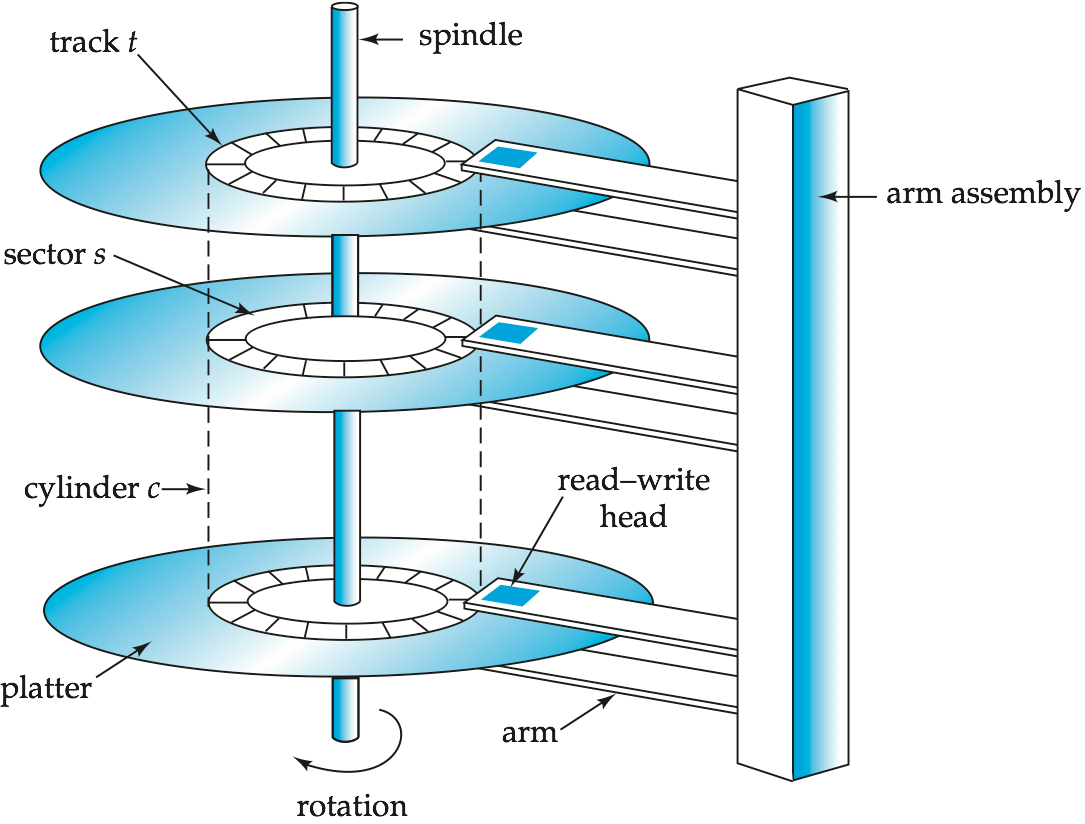
\includegraphics[scale=0.35]{img/hdd.png}
			\caption{Festplatte: Schematischer Aufbau (Quelle: \cite[S. 433]{SKS11})}
		\end{figure}
	\end{column}
	\begin{column}{.5\textwidth}
		\begin{itemize}
			\item Festplatten sind meist in mehrere einzelne Magnetplatten unterteilt
			\item Ein Zugriffsarm für jede Platte
			\item Platten sind in Spuren (Tracks) unterteilt
			\item Spuren sind in Sektoren oder Datenbl\"ocke unterteilt
			\item	Datenbl\"ocke bilden kleinste Zugriffseinheit auf der Festplatte
			\item Vertikal gestapelte Spuren hei\ss en Zylinder
		\end{itemize}
		\vspace{4em}
	\end{column}
\end{columns}
\end{frame}

\begin{frame}
\frametitle{\insertsection}
\framesubtitle{\insertsubsection}
\structure{Zugriff auf die Daten einer Festplatte}
\\[4pt]
\begin{itemize}
	\item Mittlere Zugriffszeit
	\begin{itemize}
		\item Seek Time (Schreib-Lese-Kopf in Position bringen): 6-8ms
		\item Latency (Warten, bis der richtige Sektor den Kopf passiert): 2-3ms
		\item Transferzeit (Daten von Platte in den Speicher übertragen): 15 MB/s
	\end{itemize}
	\pause
	\abs      				
	\item Daten werden \textbf{blockweise} in Hauptspeicher übertragen.
	\begin{itemize}
		\item G\"angig sind Bl\"ocke mit Gr\"o\ss en von 512 Bytes bis 8 KB.
		\item Suchen des ersten Blocks auf Platte dauert lange (\textit{SeekTime + Latency})
		\item Sind Bl"ocke konsekutiv angeordnet, k\"onnen Folgebl\"ocke direkt gelesen werden
		\item Sind Bl\"ocke nicht konsekutiv angeordnet: \textit{SeekTime + Latency} f\"ur jeden weiteren Block 
	\end{itemize}
\end{itemize}
\abs
\pause
\alert{Festplattenzugriffe / Anzahl der \textbf{Blockzugriffe} sind \textbf{teuer} und m\"ussen minimiert werden!}
\end{frame}

\section{Seiten und Datens\"atze}

\subsection{Grundlegende Betrachtungen}

\begin{frame}
\frametitle{\insertsection}
\framesubtitle{\insertsubsection}
\textbf{Seite = Dateneinheit im Speicher}
\begin{itemize}
	\item Die kleinste Dateneinheit im Speicher eines Datenbanksystems sind \textbf{Seiten}.
	\begin{itemize}
		\item Eine Seite umfasst mehrere Bl\"ocke, die in der Regel in einer Spur liegen.
	\end{itemize}
	\item Jede Relation wird in mehreren Seiten im Speicher gespeichert.
\end{itemize}
\pause
\ \\[20pt]
\textbf{Datensatz (Record) = Abbildung des logischen Tupels einer Relation im Speicher}
\begin{itemize}
	\item Ein Tupel der Relation wird in einem \textbf{Datensatz} gespeichert.
	\item Der Datensatz liegt in einer Seite und geht nicht \"uber Seitengrenzen hinaus.
	\item Ein oder mehrere Datens\"atze können in einer Seite abgelegt werden.
\end{itemize}
\end{frame}

\begin{frame}
\frametitle{\insertsection}
\framesubtitle{\insertsubsection}
\structure{Speicherung einer Relation in Seiten und Datens\"atze}
\begin{columns}	
\begin{column}{.3\textwidth}
	\begin{tabular}{|c|c|c|}\hline
		\multicolumn{3}{|c|}{\small \textbf{\texttt{Vorlesungen}}}\\\hline\hline
		\small \textbf{{\texttt{VID}}} & \small \textbf{{\texttt{Name}}} & \small \textbf{{\texttt{\ldots}}}\\\hline 
		\small 5001 & \small Grundz\"uge & \small \ldots\\\hline 
		\small 4052 & \small Logik & \small \ldots\\\hline 
		\small 5041 & \small Ethik  & \small \ldots\\\hline 
		\small \ldots & \small \ldots & \small \ldots\\\hline 
	\end{tabular}
	\hspace{3mm}
\end{column}
\begin{column}{.48\textwidth}
	\begin{figure}
		\includegraphics[scale=0.3]{img/Seite-4711-2.png}
		\caption{Seiten mit Datens\"atzen}
	\end{figure}
\end{column}\end{columns}
\end{frame}

\begin{frame}
\frametitle{\insertsection}
\framesubtitle{\insertsubsection}
\structure{Alle I/O-Operationen der Datenbank durchlaufen den Datenbankpuffer}
\begin{itemize}
	\item Datenbankpuffer ist Teil des Hauptspeichers, der (tempor\"ar) Kopien der Seiten speichert.
	\pause
	\abs
	\item Daten der Relationen werden seitenweise von der Festplatte gelesen und auf \textit{Seiten} im Puffer geschrieben. 
	\item \textbf{DB-Operationen erfolgen ausschlie\ss lich auf den Datens\"atzen im Puffer}.
	\item Die Daten werden erst \textbf{nach Abschluss aller relevanten Operationen} auf die Festplatte zur\"uckgeschrieben.\\[6pt]
	\pause
	\abs
	\item Die Verwaltung des Puffers beinhaltet:
	\begin{itemize}
		\item Speicherreservierung und Speicherfreigabe
		\item Suchen, Ersetzen/Swapping von Seiten im Puffer
		\item Synchronisation der Pufferseiten -- im Multiuser- und Multiprogramming-Betrieb wichtig
	\end{itemize}
\end{itemize}    
\end{frame}

\begin{frame}
\frametitle{\insertsection}
\framesubtitle{\insertsubsection}
\begin{figure}
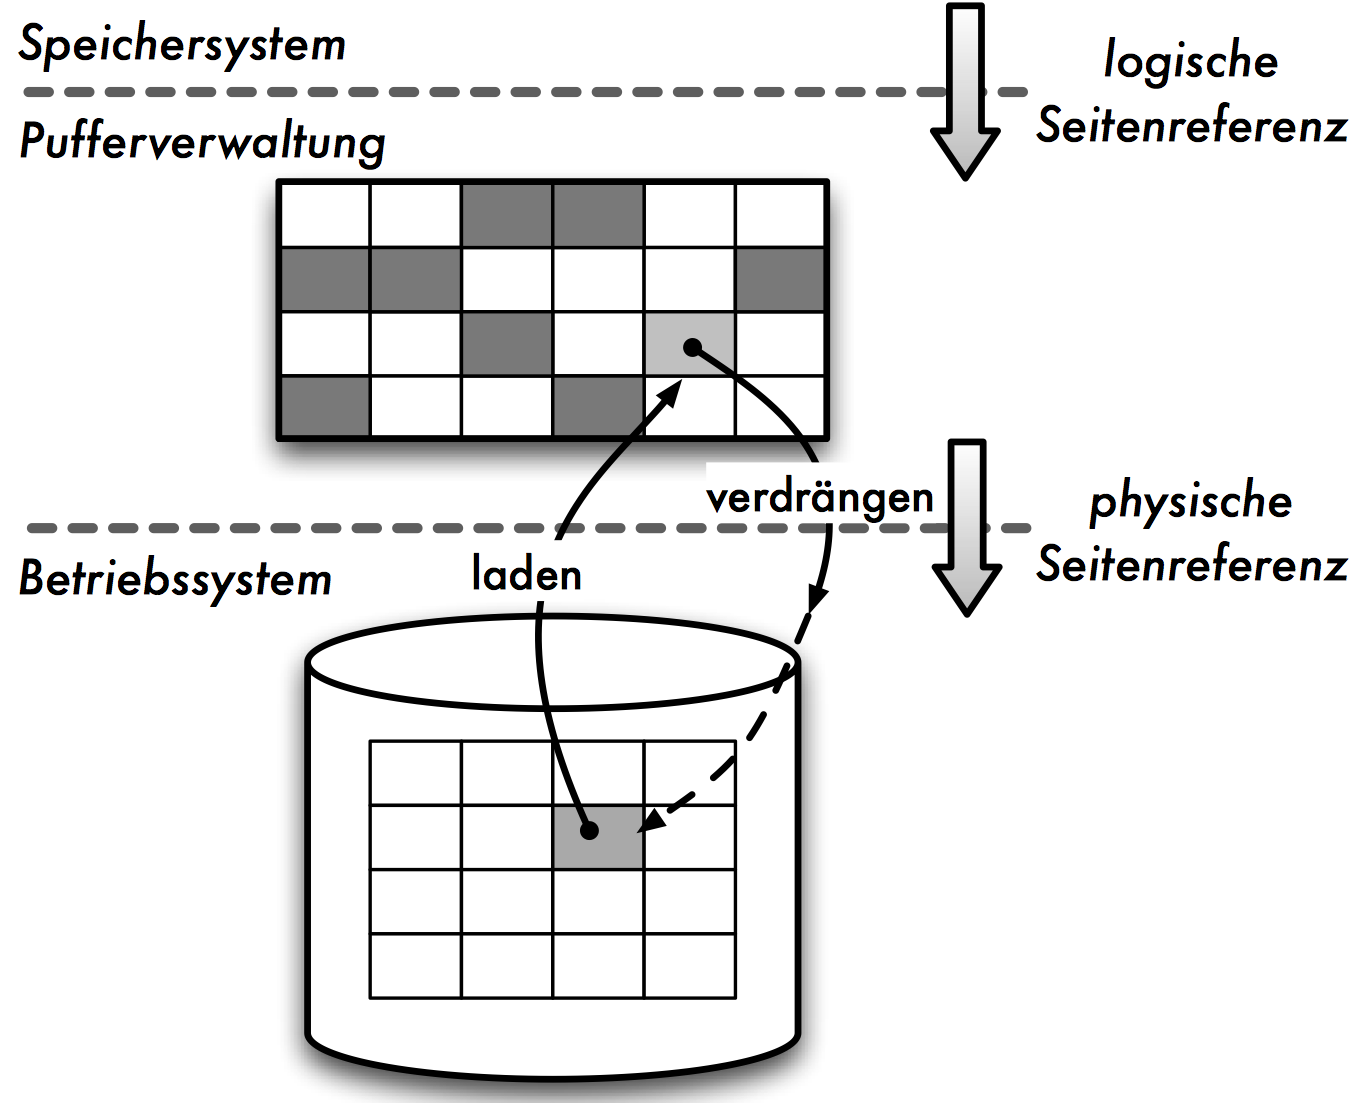
\includegraphics[scale=0.13]{img/buffer.png}
\caption{Zugriff auf Seite über Pufferverwaltung (Quelle: \cite[S. 31]{SSH11})}
\end{figure}
\end{frame}

\subsection{Aufbau eines Datensatzes}

\begin{frame}
\frametitle{\insertsection}
\framesubtitle{\insertsubsection}
\textbf{Felder eines Datensatzes}
\begin{itemize} 
	\item Ein Datensatz ist eine Sammlung von \textbf{Feldern}.
  \item Zu jedem Attribut eines Tupels einer Relation geh\"ort ein Feld des Datensatzes.
	% \item Ein Record ist eine Kollektion von Feldern, die in einer Beziehung zueinander stehen	
	\item Ein Feld speichert den Wert des entsprechenden Attributs des Tupels.\\[20pt]
	\item Jedes Feld wird durch ein oder mehrere Bytes repräsentiert.
	\item Die Felder sind typisiert (\texttt{bool, int} etc.).
  %	\item Alle Felder und ihre zugehörigen Datentypen bestimmen den Recordtyp
	\pause
	\item Zu gro\ss e Attributwerte (z.~B.~Bilder) werden i.~d.~R.~ausgelagert:
	\begin{itemize}
		\item Daf\"ur existieren spezielle Datentypen:
		\begin{itemize}
			\item Binary Large Object (\texttt{BLOB}) für Binärdaten (Bilder, Musik etc.)
			\item Character Large Object (\texttt{CLOB}) für Textdaten (Fliesstexte, Webseiten etc.)
		\end{itemize}  
		\item Es wird nur eine Referenz (Pointer) im Feld gespeichert
		\item Die Daten selbst werden aus der Seite ausgelagert
	\end{itemize}	
\end{itemize}
\end{frame}

\begin{frame}
	\frametitle{\insertsection}
	\framesubtitle{\insertsubsection}
 \begin{itemize}
	\item Datens\"atze werden durch folgende Typen klassifiziert:
	\begin{itemize}
		\item 'Fixed Length Records' oder 'Fixl\"angen-Speicherung': Datens\"atze haben immer die gleiche L\"ange, auch wenn reservierter 
		Speicher ggf.~nicht verwendet wird.
		\item 'Variable Length Records' oder 'Speicherung in variabler L\"ange': Datens\"atze belegen nur den tats\"achlich verwendeten 
		Speicher.
	\end{itemize}
\end{itemize}    
\end{frame}

\begin{frame}[fragile]
	\frametitle{\insertsection}
	\framesubtitle{\insertsubsection}
\begin{columns}
\begin{column}{.48\textwidth}
    \structure{Struktur eines Fix-Length-Datensatzes}
    \lstset{language=c}
    \begin{lstlisting}[xleftmargin=3ex]
struct mitarbeiter {
  char name[30];
  char ssn[9];
  int salary;
  int job_code;
  char department[20];
} ;
    \end{lstlisting}
\end{column}
\begin{column}{.48\textwidth}
    \structure{Struktur eines Variable-Length-Datensatzes}
    \lstset{language=C}
    \begin{lstlisting}[xleftmargin=3ex]
struct mitarbeiter {
  char* name; /* Pointer */
  char ssn[9];
  int salary;
  int job_code;
  char* department /* Pointer */;
} ;
    \end{lstlisting}
\end{column}
\end{columns}
\end{frame}

\subsection{Abbildung im Hauptspeicher}

\begin{frame}
	\frametitle{\insertsection}
	\framesubtitle{\insertsubsection}
	\structure{Fixl\"angen-Speicherung}
	\begin{itemize}
		\item F\"ur jedes Feld wird im Speicher eine feste Anzahl von Bytes reserviert 
		\item Vorteil: Sehr einfache und schnelle Adressierung
		\item Nachteil: Unflexibel bez\"uglich \"Anderung der Datengr\"o\ss e
	\end{itemize}	
	 \begin{figure}
	 	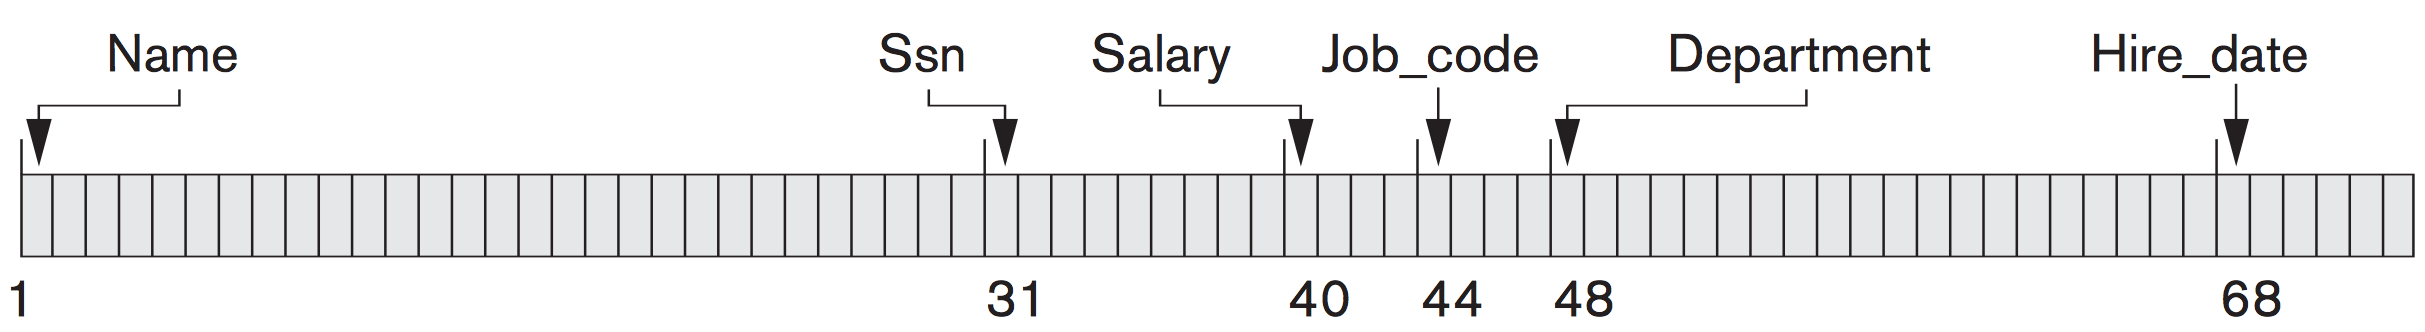
\includegraphics[scale=0.13]{img/fix.png}
	 	\caption{Fixlängen-Speicherung (Quelle: \cite[S. 596]{EN10})}
	 \end{figure}
\end{frame}

\begin{frame}
	\frametitle{\insertsection}
	\framesubtitle{\insertsubsection}
	\structure{Speicherung in variabler L\"ange -- Alternative 1}
	\begin{itemize}
		\item Zwischen Feldern variabler L\"ange wird ein spezielles Trennzeichen gesetzt. 
		\item Vorteil: Keine Speicherplatzverschwendung und flexibel bez\"uglich Datengr\"o\ss e.
		\item Nachteil: Langsamerer Zugriff als bei Fixl\"angen.
	\end{itemize}	
	\begin{figure}
		\includegraphics[scale=0.13]{img/var.png}
		\caption{Speicherung in variabler L\"ange -- Alternative 1 (Quelle: \cite[S. 596]{EN10})}
	\end{figure}
\end{frame}

\begin{frame}
	\frametitle{\insertsection}
	\framesubtitle{\insertsubsection}
	\structure{Speicherung in variabler L\"ange -- Alternative 2}
	\begin{itemize}
		\item Speicherung als Key-Value-Paare
		\item Nicht gesetzte Felder werden nicht mehr explizit gespeichert. 
		\item Vorteil: Es wird nur noch der minimal notwendige Speicherplatz belegt.
		\item Nachteil: Auslesen der Key-Value-Paare aufw\"andig.
	\end{itemize}
	\begin{figure}
		\includegraphics[scale=0.13]{img/var2.png}
		\caption{Speicherung in variabler L\"ange, Alternative 2 (Quelle: \cite[S. 596]{EN10})}
	\end{figure}
\end{frame}

\subsection{Abbildung im Hauptspeicher -- Dateien und Bl\"ocke}

\begin{frame}
	\frametitle{\insertsection}
	\framesubtitle{\insertsubsection}
    \structure{Organisationsformen \textit{Unspanned} und \textit{Spanned}}
    \begin{itemize}
    	\item DB-Dateien bestehen aus Sequenzen von Datens\"atzen: Datens\"atze werden in Dateien geschrieben.
      \item Datens\"atze innerhalb einer Datei sind (normalerweise) vom gleichen Relationentyp.
      \pause
      \item Die Datens\"atze werden in einer Datei in Bl\"ocken im Unspanned- bzw.~im Spanned-Modus gespeichert ...
    \end{itemize}
\end{frame}

\begin{frame}
\frametitle{\insertsection}
\framesubtitle{\insertsubsection}
\structure{Organisationsformen \textit{Unspanned} und \textit{Spanned}}
\abs
\emph{Unspanned}: Pro Block werden nur ein oder mehrere vollst\"andige Datens\"atze gespeichert
	\begin{itemize}
		\item Ungenutzter Speicherplatz am Ende eines Blocks
	\end{itemize}
  \begin{figure}
	 \includegraphics[width=200pt]{img/unspanned.png}
	 \caption{Unspanned (Quelle: \cite[S. 598]{EN10})}
  \end{figure}
\end{frame}


\begin{frame}
\frametitle{\insertsection}
\framesubtitle{\insertsubsection}
\structure{Organisationsformen \textit{Unspanned} und \textit{Spanned}}
\abs
\emph{Spanned}: Es können auch nur Teile eines Datensatzes in einem Block gespeichert werden. 
	\begin{itemize}
		\item Am Ende eines Blocks wird ein Pointer auf den nachfolgenden Block gesetzt.
		\item Ein Datensatz kann sich \"uber mehrere Bl\"ocke '\textit{spannen}'.
		\item Stets zu verwenden, wenn die Datens\"atze gr\"o\ss er als die Bl\"ocke sind. 
	\end{itemize}
  \begin{figure}
 	 \includegraphics[width=200pt]{img/spanned.png}
	 \caption{Spanned (Quelle: \cite[S. 598]{EN10})}
  \end{figure}
\end{frame}

\begin{frame}
\frametitle{\insertsection}
\framesubtitle{\insertsubsection}
\begin{definition}[Blocking Factor]
	Für gegebene effektive Blockgr\"o\ss e $B$ und L\"ange der Datens\"atze $R$ ist der Blocking Factor gegeben durch:
	$$bfr = \left \lfloor \frac{B}{R}\right \rfloor$$
\end{definition}
\pause
\ \\[-18pt]
\begin{block}{\textbf{Bemerkung}}
	\begin{itemize}
		\item \textit{bfr} gibt maximale Anzahl vollst\"andiger Datens\"atze pro Block an.
		\item In der Organisationsform 'Unspanned' bleiben $B-(bfr \cdot R)$ Bytes pro Block ungenutzt, und es werden
		$\left \lceil \frac{n}{bfr}\right \rceil$ Bl\"ocke für die Speicherung von $n$ Datens\"atzen ben\"otigt. \textbf{Warum?}
	\end{itemize} 
\end{block}
\pause
\ \\[-8pt]
\textbf{Beispiel:}
$B=512,\ R=120 \Rightarrow bfr = \left\lfloor\frac{512}{120}\right\rfloor = 4$. Im Unspanned-Modus
bleiben somit $512-(4 \cdot 120)=32$ Bytes pro Block ungenutzt. F\"ur $n=250$ Datens\"atze werden 
dann $\left \lceil \frac{250}{4}\right \rceil = 63$ Bl\"ocke ben\"otigt.
\end{frame}

\subsection{Speicherung von Dateien}

\begin{frame}
\frametitle{\insertsection}
\framesubtitle{\insertsubsection}
\structure{Verschiedene Verfahren zur Speicherung zusammengeh\"orender Bl\"ocke auf der Festplatte:}
\abs
\textbf{Contiguous Allocation}
	\begin{itemize}
		\item Alle Bl\"ocke werden konsekutiv hintereinander geschrieben
		\item Vorteil: Hohe Lesegeschwindigkeit
		\item Nachteil: Teure Einf\"ugeoperationen
	\end{itemize}\ \\[4pt]
\begin{figure}
	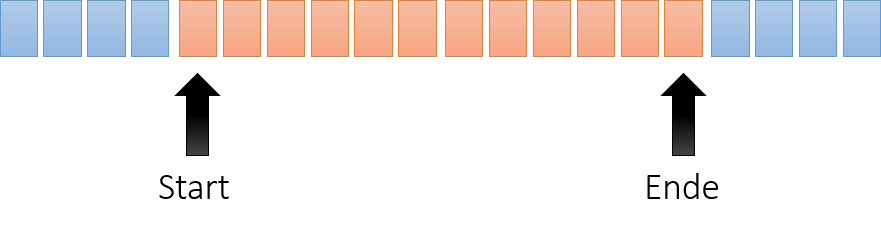
\includegraphics[width=200pt]{img/cont.png}
\end{figure}
\end{frame}

\begin{frame}
\frametitle{\insertsection}
\framesubtitle{\insertsubsection}
\structure{Verschiedene Verfahren zur Speicherung zusammengeh\"orender Bl\"ocke auf der Festplatte}
\abs
\textbf{Linked Allocation}
	\begin{itemize}
		\item Am Ende jedes Blocks befindet sich ein Pointer auf den n\"achsten Block
		\item Vorteil: Einf\"ugeoperationen problemlos realisierbar
		\item Nachteil: Teure Leseoperationen
	\end{itemize}\ \\[4pt]
\begin{figure}
	\includegraphics[width=200pt]{img/linked.png}
\end{figure}
\end{frame}

\begin{frame}
\frametitle{\insertsection}
\framesubtitle{\insertsubsection}
\structure{Verschiedene Verfahren zur Speicherung zusammengeh\"orender Bl\"ocke auf der Festplatte}
\abs
\textbf{Clustered Allocation}
	\begin{itemize}
		\item Konsekutive Block-Cluster werden untereinander verlinkt
		\item Kompromissl\"osung zwischen Contiguous Allocation und Linked Allocation
	\end{itemize}
\begin{figure}
	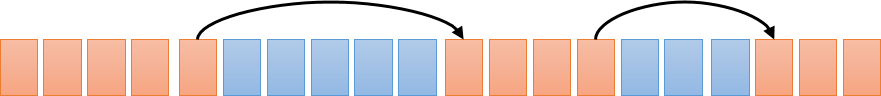
\includegraphics[width=200pt]{img/clustered.png}
\end{figure}
\end{frame}

\section{Formen der Dateiorganisation}
\subsection{Heap-Dateien}

\begin{frame}
	\frametitle{\insertsection}
	\framesubtitle{\insertsubsection}
	\structure{\textbf{Heap-Dateien}}\\[4pt]
	\begin{itemize}
		\item In einer Heap-Datei werden die Datens\"atze unsortiert sequentiell auf dem Datenträger gespeichert.\\[4pt]
		\item Neue Einträge werden ans Ende der Datei angeh\"angt. Stichwort: \textit{append}-Operation.\\[4pt]
		\item Die Adresse des letzten Blocks/der letzten Seite der Datei ist im Datei-Header abgespeichert.
	\end{itemize}	
\end{frame}

\begin{frame}
\frametitle{\insertsection}
\framesubtitle{\insertsubsection}
\structure{\textbf{Einf\"ugen in einer Heap-Datei}}	
\begin{itemize}
	\item Erster Datei-Block wird in den Hauptspeicher geladen.\\[4pt]
	\item Aus den Header-Informationen wird der letzte Block der Datei identifiziert.\\[4pt]
	\item Letzter Block der Datei wird in den Hauptspeicher geladen. \\[4pt]
	\item Ein neuer Datensatz wird in den letzten Block geschrieben. \\[4pt]
	\item Falls nicht mehr genug Platz im letzten Block vorhanden ist, wird ein neuer Block erzeugt.\\[4pt]
	\item Block wird auf Platte zur\"uck geschrieben -- ggf.~Update der Adresse des letzten Blocks im Header.\\[4pt]
\end{itemize}
\pause
Fazit: Einf\"uge-Operationen sehr effizient, da immer nur am Ende angeh\"angt wird.
\end{frame}

\begin{frame}
\frametitle{\insertsection}
\framesubtitle{\insertsubsection}
\structure{\textbf{Lesen/\"Andern in einer Heap-Datei}}	
\begin{itemize}
	\item Der Bestand wird Seite für Seite nach Treffern abgesucht. 
	\item Ggf.~\"Andern und R\"uckschreiben des modifizierten Blocks auf die Platte.
	\item Ggf.~muss die Datei bis zum Ende gelesen werden.
	\item Suchoperation ist linear zur Anzahl der Bl\"ocke/Seiten: $O(n)$. $\frac{n}{2}$ im Durchschnitt.
\end{itemize}
\end{frame}

\begin{frame}
\frametitle{\insertsection}
\framesubtitle{\insertsubsection}
\structure{\textbf{L\"oschen in einer Heap-Dateien}}
\begin{itemize}
	\item Lesen des relevanten Blocks in den Hauptspeicher 
	\item L\"oschen des in Frage kommenden Datensatzes 
	\item R\"uckschreiben des (leeren) Blocks auf die Platte
\end{itemize}
\abs
\pause
\alert{Dadurch wird Datei stark fragmentiert. Es entstehen Lücken, die Speicherplatz verschwenden.}
\end{frame}

\begin{frame}
\frametitle{\insertsection}
\framesubtitle{\insertsubsection}
\structure{\textbf{L\"oschen in einer Heap-Dateien} -- R\"uckschreiben des Blocks}
\begin{itemize}
\item Alternative 1: Verwendung eines Deletition-Markers, mit dem ein Datensatz als \textit{gel\"oscht} markiert wird.
\begin{itemize}
	\item Damit kann eine \textit{Papierkorb-Semantik} realisiert werden. Gel\"oschte Datens\"atze k\"onnen wiederhergestellt werden
\end{itemize}
\pause
\ \\[4pt]
\item Alternative 2: Tats\"achliches L\"oschen. Einf"ugen neuer Datens\"atze erfolgt in den entstandenen L\"ucken, 
da Heap-Datei ohnehin nicht sortiert ist.
\begin{itemize}
	\item Erfordert eine Art Buchhaltung, an welcher Stelle L\"ucken in passender Größe existieren.
	\item Kann in Kombination mit Alternative 1 verwendet werden.
\end{itemize} 
\end{itemize}
\abs
\pause
\alert{Beide Varianten benötigen regelmäßige Datei-Reorganisationen!}
\end{frame}

\begin{frame}
\frametitle{\insertsection}
\framesubtitle{\insertsubsection}
\structure{\textbf{Besondere Eigenschaft von Heap-Dateien}}\\[4pt]
Werden Datens\"atze mit Fixl\"angen im Unspanned-Modus gespeichert, kann auf einen Datensatz an Position $i$ in der Datei 
folgenderma\ss en zugegriffen werden: 
\abs
Der $i$-te Datensatz befindet sich im Block $\left \lfloor\frac{i}{bfr}\right\rfloor$ und ist dort an der Position $i\mod bfr$. 
\textbf{Warum?}
\abs\ \abs
\pause
\alert{Beachte: Dieser Zugriff in der unsortierten Heap-Datei beschleunigt lediglich das Suchen nach dem 
	$i$-ten Eintrag der Datei, nicht aber die Suche anhand konkreter Felder in den Datens\"atzen.}
\end{frame}

\subsection{Sortierte Dateien}

\begin{frame}
\frametitle{\insertsection}
\framesubtitle{\insertsubsection}
\structure{\textbf{Sortierte Dateien}}
\begin{itemize}
	\item In einer sortierten Datei werden die Datens\"atze anhand eines Sortierfelds sequentiell gespeichert.
	\item Besitzt Sortierfeld Schlüsseleigenschaften -- und ist daher eindeutig --, so wird es als Sortierschl\"ussel bezeichnet.
	\item Auch zusammengesetzte Sortierfeld, z.~B.~\texttt{(Nachname, Vorname)}, ist m\"oglich.
\end{itemize}
\end{frame}

\begin{frame}
	\frametitle{\insertsection}
	\framesubtitle{\insertsubsection}
	\structure{\textbf{Sortierte Dateien}}
\abs
	\structure{Vorteile}
	\begin{itemize}
		\item Lesezugriffe in Sortierreihenfolge sind sehr effizient.
		\item Suche über den Sortierschl\"ussel kann effizient abgebildet werden: Binäre Suche in $O(\log_2 n)$ f\"ur $n$ Datens\"atze.
	\end{itemize}
\abs
\pause
	\structure{Nachteile}
	\begin{itemize}
		\item Teure Einf\"uge- und L\"oschoperationen
		\item Aufwand wie bei Heap-Datei, wenn Sortierschl\"ussel nicht verwendet wird
	\end{itemize}
\end{frame}

\begin{frame}
\frametitle{\insertsection}
\framesubtitle{\insertsubsection}
\begin{columns}
	\begin{column}{.4\textwidth}
		\includegraphics[width=170pt]{img/Record-Block-Storing-4.png}
	\end{column}	
	\begin{column}{.55\textwidth}
		\structure{\textbf{Beispiel}}
		\begin{itemize}
			\item Sortierfeld: Name 
			\item Alphabetisch aufsteigende Reihenfolge in den Bl\"ocken
			\item Mittels bin\"arer Suche effizientes Auffinden eines Datensatzes m\"oglich
			\item Einf\"ugen muss Sortierung ber\"ucksichtigen
		\end{itemize}
	\end{column}
\end{columns}
\end{frame}

\begin{frame}
\frametitle{\insertsection}
\framesubtitle{\insertsubsection}
\structure{Sortierte Datei mit Pointer}\\[4pt]
\begin{itemize}
	\item Datens\"atze enthalten Pointer, der auf n\"achsten Datensatz in Sortierreihenfolge verweist.
\end{itemize}
\begin{center}
\begin{figure}
	\includegraphics[scale=0.35]{img/seq1.png}
	\caption{Sortierte Datei mit Pointer (Quelle: \cite[S. 458]{SKS11})}
\end{figure}
\end{center}
\end{frame}

\begin{frame}
\frametitle{\insertsection}
\framesubtitle{\insertsubsection}	
\structure{Sortierte Datei mit Pointer}\\[4pt]
\begin{itemize}
\item Einf\"ugen eines Datensatzes.
\end{itemize}
\begin{center}
\begin{figure}
\includegraphics[scale=0.45]{img/seq2.png}
\caption{Einf\"ugeoperation in sortierter Datei mit Pointer (Quelle: \cite[S. 459]{SKS11})}
\end{figure}
\end{center}
\end{frame}

\begin{frame}
\frametitle{\insertsection}
\framesubtitle{\insertsubsection}
\structure{Sortierte Datei mit Pointer}\\[4pt]
\textbf{Vorteil}
\begin{itemize}
\item Minimierung des Einf\"uge-Overheads.
\item Einf\"ugeoperationen k\"onnen deutlich schneller durchgef\"uhrt werden.
\end{itemize}
\abs
\pause
\textbf{Nachteil}
\begin{itemize}
\item Daten der Datei werden ggf.~\"uber unterschiedliche Bl\"ocke/Seiten verteilt.
\item Dadurch zusätzlicher Suchaufwand erforderlich. Reorganisation auch hier notwendig.
\end{itemize}
\end{frame}

\subsection{Hash-Dateien}

\begin{frame}
\frametitle{\insertsection}
\framesubtitle{\insertsubsection}
\structure{\textbf{Hash-Dateien}}\\[4pt]
\abs
Idee: 
\begin{itemize}
	\item Wert eines bestimmten Feldes (Hash-Feld) des Datensatzes auf eine \textit{Bucket}-Nummer abbilden.
	\item Bucket besteht aus Datenbankseiten der Relation.		
	\item Im Bucket mit der entsprechenden Bucket-Nummer wird der zugeh\"orige Datenzatz gespeichert.
	\item Abbildung zwischen Hash-Feld des Datensatzes und Bucket-Nummer mittels einer Hash-Funktion.  
	\item Ein oder mehrere Hash-Felder m\"oglich.
\end{itemize}	
\end{frame}

\begin{frame}
\frametitle{\insertsection}
\framesubtitle{\insertsubsection}
\structure{\textbf{Hash-Dateien}}\\[4pt]
Idee: 
\begin{figure}
\includegraphics[scale=0.35, trim=0 0 0 4cm]{img/Hash-Bucket-0.png}
\\[-8pt]\caption{Mapping der Datens\"atze auf Buckets}
\end{figure}
\end{frame}

\begin{frame}
\frametitle{\insertsection}
\framesubtitle{\insertsubsection}
\structure{\textbf{Hash-Dateien}}\\[4pt]
\abs
Umsetzung: 
\begin{itemize}
	\item Einer Relation wird Speicherbereich von $p$ Buckets (Seiten) mit logischen Adressen $0, 1,\ldots, {p\text{\,--\,}1}$ zugeordnet. 
	\item Wertebereich (Dom\"ane) $S$ der Hash-Felder wird durch Hash-Funktion $h$ direkt auf eine Bucket-Adresse abgebildet. 
	$$h:S\to\{0, 1,\ldots, {p\text{\,--\,} 1}\},\quad s\mapsto h(s)\in\{0, 1,\ldots, {p\text{\,--\,} 1} \}$$
	In der Regel $\vert S\vert\gg p$, und somit $h$ \textbf{nicht} injektiv.
	\item Gebr\"auchlichste Art der Hash-Funktion: \emph{Division mit Rest} und meistens $p$ Primzahl.
	$$h(s) \equiv s\mod p$$
\end{itemize}		
\end{frame}

\begin{frame}
\frametitle{\insertsection}
\framesubtitle{\insertsubsection}
\structure{\textbf{Hash-Dateien}}\\[4pt]
Umsetzung: 
\begin{figure}
\includegraphics[scale=0.35, trim=0 0 0 4cm]{img/Hash-Bucket-1.png}
\\[-8pt]\caption{Mapping der Datens\"atze auf Buckets mit Hash-Funktion}
\end{figure}
\end{frame}

\begin{frame}
\frametitle{\insertsection}
\framesubtitle{\insertsubsection}
\structure{\textbf{Hash-Dateien}}\\[4pt]
\abs
Umsetzung Offenes Hashing: 
\begin{itemize}
	\item Ist beim Schreiben in der Seite des Bucket nicht genügend Platz, muss eine \"Uberlaufseite angelegt werden.
	\item Es wird ein Pointer in der vollen Seite auf die neue \"Uberlaufseite gespeichert.
	\item Eine \"Uberlaufseite kann wiederum \"uberlaufen, etc.
\end{itemize}		
\end{frame}

\begin{frame}
\frametitle{\insertsection}
\framesubtitle{\insertsubsection}
\structure{\textbf{Hash-Dateien}}\\[4pt]
Umsetzung: 
\begin{figure}
\includegraphics[scale=0.35, trim=0 0 0 4cm]{img/Hash-Bucket-3.png}
\\[-8pt]\caption{Mapping der Datens\"atze auf Buckets mit \"Uberlaufseite}
\end{figure}
\end{frame}

\begin{frame}
\frametitle{\insertsection}
\framesubtitle{\insertsubsection}
\structure{\textbf{Lesen in Hash-Dateien}}
\begin{itemize}
	\item Aus dem Feldwert wird m.~H.~der Hash-Funktion die Adresse der Seite und des Satzes direkt ermittelt. 
	\item Bei \"Uberl\"aufen muss die Kette linear abgearbeitet werden. 
	\item Ohne \"Uberlaufseiten kann auf jeden Datensatz in konstanter Zeit zugegriffen werden.
	\item Sehr schneller Zugriff.	
\end{itemize}
\end{frame}

\begin{frame}
\frametitle{\insertsection}
\framesubtitle{\insertsubsection}
\structure{\textbf{Schreiben in Hash-Dateien}}
\begin{itemize}
	\item Hash-Funktion liefert die Adresse des zugeordneten initialen Blocks.
	\item Bei \"Uberl\"aufen muss die Kette linear abgearbeitet werden. 
	\item Falls nicht gen\"ugend Platz vorhanden ist, wird eine neue \"Uberlaufseite angelegt, in die der Datensatz geschrieben wird.
\end{itemize}
\end{frame}

\begin{frame}
\frametitle{\insertsection}
\framesubtitle{\insertsubsection}
\structure{\textbf{L\"oschen in Hash-Dateien}}
\begin{itemize}
	\item Der betreffende Datensatz wird gesucht -- wie beim Lesen -- und aus dem Block eliminiert oder zum L\"oschen markiert. 
	\item Falls eine Überlaufseite leer wird, kann sie wieder freigegeben werden.
\end{itemize}
\end{frame}

% Speichereffizienz	HASH-Speicherstrukturen benötigen keine zusätzlichen Verwaltungsdaten. 
% Der Primärbereich muss ausreichend groß angelegt werden, damit neue Daten Platz finden und die Überlaufseiten nicht ausarten. 
% Bei veränderlichen Datenbeständen ist die Speichereffizienz niedrig.

\begin{frame}[t]
\framesubtitle{Gegenüberstellung: Heap -- Sortiert -- Hash}
{\small
	\begin{center}
		\begin{tabular}{|l|p{3cm}|p{3cm}|p{3cm}|}\hline
			& \textbf{Heap-Datei} & \textbf{Sortierte Datei} & \textbf{Hash-Datei}\\\hline
			Suchoperationen & Aufwändig. Alle S\"atze m\"ussen gelesen werden: $O(n)$, Durchschnitt $\frac{n}{2}$ 
			& Weniger aufwändig. Binäre Suche: $O(\log_2 n)$ & Nach Hash-Wert-Berechnung sehr schneller Zugriff\\\hline
			Einfügeoperationen & Schnell: Neuer Satz wird am Ende der Datei angeh\"angt 
			& Aufwändig. Dateien m\"ussen ggf.~umorganisiert werden 
			& Neuer Satz wird am Ende der Seite angeh\"angt. Ggf.~Erzeugen neuer \"Uberlaufseite\\\hline
			Löschoperationen & Aufwändig. Datensatz muss gesucht werden, Löschen hinterlässt Lücken, Reorganisation erforderlich 
			& M.~H.~von Sortierfeld günstiger. Ansonsten wie unsortierte Datei. Reorganisation erforderlich. 
			& \"Ahnlich wie bei Heap-Dateien\\\hline
			Sortierte Ausgabe & Sehr aufwändig & Sehr einfach & Sehr aufwändig \\\hline
		\end{tabular}
	\end{center}
}
\end{frame}

\section*{Übungsaufgaben}
\begin{frame}[t]
\frametitle{\insertsection}
\begin{alertblock}{Grundlagen der Datenspeicherung}
\begin{enumerate}
	\nowrite{ 
		\item Gegeben ist ein Datenschema \texttt{Kunde(\uline{KNR}, Vorname, Nachname, PLZ, Ort)}. Implementieren Sie ein Java-Programm, welches
		\begin{itemize}
			\item Eine Menge von Kundendatensätzen auf Festplatte speichern und wieder einlesen kann,
			\item einen Datensatz anhand der Kundennummer sucht,
			\item Datensätze anhand der PLZ sucht und
			\item Datensätze anhand des Nachnamens sucht, wobei Wildcards möglich sind (z.\,B. \texttt{Schmi*}).
		\end{itemize}
	}			
	\item Erläutern Sie, auf welche Weise Daten von der Festplatte in den Hauptspeicher übertragen werden.
	Gehen Sie in Ihren Erläuterungen nicht nur auf den Aufbau der Platte, sondern auch auf den Begriff der \textit{mittleren Zugriffszeit} ein.			
	\item Erl\"autern Sie den Begriff des \textit{Datensatzes} sowie den Begriff einer \textit{Datei}
	und erläutern Sie die drei aus der Vorlesung bekannten Speicherverfahren jeweils für Datens\"atze fester L\"angen und variable L\"angen 
	anhand eines Beispiels.			
\end{enumerate}
\end{alertblock}
\end{frame}

\begin{frame}[t]
\frametitle{\insertsection}	
\begin{alertblock}{Grundlagen der Datenspeicherung (forts.)}
\begin{enumerate}
\setcounter{enumi}{3}
\item Berechnen Sie den Blocking Factor für eine Blockgröße $b=1024$ und eine Satzlänge $r=327$.  
Wie viele Bl\"ocke werden für die Speicherung von 1000 S\"atzen ben\"otigt?
\item Durch die Abrundungsoperation bei der Berechnung von $\mathit{bfr}$ kann ggf.~das Ergebnis $\mathit{bfr}=0$ entstehen. 
Welche Aussage hat dieses Ergebnis und welche Konsequenz ergibt sich daraus?
\item In einer Heap-Datei wird der $i$-te Datensatz in den Festplattenblock
$$\left\lfloor{\frac{i}{\mathit{bfr}}}\right\rfloor,\quad \mathsf{Position~} (i \bmod \mathit{bfr})$$
gespeichert. Erl\"autern Sie, warum dieses Wissen im operativen Datenbankbetrieb faktisch nicht vorteilhaft ausgenutzt werden kann.
\end{enumerate}
\end{alertblock}
\end{frame}

%!TEX root = Slides.tex
\part{Indizes und Hashverfahren}

\section{Grundlagen Indizes}

\begin{frame}{Motivation}
\framesubtitle{Analogie: Index eines Buches}
\structure{\textbf{Daumenindex}}
\\[4pt]
\begin{columns}
	\begin{column}{.2\textwidth}
		\includegraphics[scale=0.32]{img/index1.png}
	\end{column}
	\begin{column}{.7\textwidth}
		\begin{itemize}
			\item Daumenindex ordnet logisch zusammenh\"angende Inhalte (Datenwerte) den Abschnitten des Buches (Adressen) zu.
			\item Jedem logischen Inhalt wird ein Abschnitt zugewiesen.
			\item Die Inhalte sind im Daumenindex sortiert/geordnet.
		\end{itemize}
	\end{column}
\end{columns}
\end{frame}

\begin{frame}{Motivation}
\framesubtitle{Analogie: Index eines Buches}
\structure{\textbf{Sachindex}}
\\[4pt]
\begin{columns}
\begin{column}{.33\textwidth}
	\includegraphics[scale=0.4]{img/index2.png}
\end{column}
\begin{column}{.67\textwidth}
	\begin{itemize}
		\item Sachindex ordnet Sachbegriffe (Datenwerte) den Seitenzahlen (Adressen) zu. 
		\item Jedem Sachbegriff k\"onnen mehrere Seitenzahlen zugewiesen werden.
		\item Die Sachbegriffe sind im Sachindex sortiert/geordnet.
	\end{itemize}
\end{column}
\end{columns}
\end{frame}

\begin{frame}{\insertsection}
\framesubtitle{\insertsubsection}	
\begin{definition}[Index]
	Ein Index einer Relation ist eine zus\"atzliche Datenstruktur, die einen effizienten Zugriff auf die Datens\"atze der Relation
	erm\"oglicht. 
	\pause
	\begin{itemize}
		\item Ein Index besteht aus bestimmten Index-Feldern und Adressfeldern.
		\item	Die Index-Felder entsprechen Feldern der Relation. 
		\item Die Werte der Index-Felder bestimmen die Adressen der Seiten der Relation, die die Datens\"atze 
		mit den entsprechenden Feldwerten enthalten. 
	\end{itemize}
\end{definition}		
\end{frame}

\begin{frame}{\insertsection}
\framesubtitle{\insertsubsection}
\begin{figure}
	\includegraphics[scale=0.4]{img/IndexSchema.png}
	\\[-10pt]\caption{Indexstruktur und Relationenschema}
\end{figure}
\end{frame}

\begin{frame}{\insertsection}
\framesubtitle{\insertsubsection}
\begin{figure}
\includegraphics[scale=0.4]{img/IndexPageRelation.png}
\\[-10pt]\caption{Index und Seiten der Relation}
\end{figure}
\end{frame}

\begin{frame}{\insertsection}
\framesubtitle{\insertsubsection}	
\begin{block}{\textbf{Bemerkung}}
	\begin{itemize}
		\item Index wird über einem oder mehreren Feldern (Attributen) der Relation gebildet.
		\item Beliebige Attribute können zur Erstellung des Index herangezogen werden.
		\pause
		\item Index ist zus\"atzliche Datenstruktur, die effizienten Zugriffspfad auf Datens\"atze erm\"oglicht.  	
		\item Index ben\"otigt zus\"atzlichen Speicherbedarf und Aufwand bei Indexverwaltung.				
	\end{itemize}
\end{block}
\abs
\begin{block}{\textbf{Bemerkung}}
	\begin{itemize}
		\item Index-Typen: Dense Index und Sparse Index
		\item Index-Arten: Prim\"arindex und Sekund\"arindex
		\item Index-Klassen: 
		\begin{itemize}
			\item Einstufige und mehrstufige Indizes
			\item B\"aume
			\item Hashing
		\end{itemize}
	\end{itemize}
\end{block}
\end{frame}

\begin{frame}[label=sparsedense]{\insertsection}
\framesubtitle{\insertsubsection}
\structure{Index-Typen}
\abs
Ein Index speichert
\begin{itemize}
	\item die Werte der Index-Felder in sortierter/geordneter Reihenfolge.
	\begin{itemize}
		\item Effiziente Sortierverfahren können angewendet werden
		\item Sequentielle Suche entfällt
	\end{itemize}
	\item eine Menge von zugeh\"origen Adressen auf die Seiten (Bl\"ocke), in denen ein Datensatz mit dem entsprechenden Wert 
	der Felder vorhanden ist. 
\end{itemize}
\pause
\structure{Zwei grundlegende Index-Typen:}
\begin{itemize}
	\item \textit{Dense Index}: Ein Eintrag im Index f\"ur jeden Feld-Wert der Relation
	\item \textit{Sparse Index}: Nur einige Datens\"atze der Relation sind im Index repr\"asentiert. Es existieren Werte-L\"ucken. 
	\begin{itemize}
		\item Notwendige Voraussetzung für einen Sparse Index: nach dem Suchfeld sortierte/geordnete und ggf.~verpointerte Datens\"atze in der
		Relation.
	\end{itemize}
\end{itemize}
\end{frame}

\begin{frame}{\insertsection}
\framesubtitle{\insertsubsection}	
\structure{Index-Arten}
\abs
\textbf{Prim\"arindex}
\begin{itemize}
	\item Prim\"arindex legt neben effizientem Zugriff auch physische Sortierung/Anordnung der 
	indizierten Relation fest.\\[4pt]
	\item Prim\"arindex und Relation sind nach den gleichen Feldern sortiert/geordnet.
	\item F\"ur jede Relation gibt es somit nur einen Prim\"arindex.\\[4pt]
	\item In der Regel wird der Prim\"arschl\"ussel der Relation als Index-Feld verwendet.
\end{itemize}
\pause
\abs
\textbf{Beispiel:} In Mitarbeitertabelle kann Mitarbeiter mit Prim\"arindex f\"ur Schl\"ussel
\texttt{MID} schnell gefunden werden, ohne alle Datens\"atze der Relation direkt zu lesen.	
\\[4pt]
\pause
Beachte: Relation und Prim\"arindex werden \"uber \texttt{MID} sortiert/geordnet gespeichert.
\end{frame}

\begin{frame}{\insertsection}
\framesubtitle{\insertsubsection}	
\structure{Index-Arten}
\abs
\textbf{Sekund\"arindizes}
\begin{itemize}
	\item sind Indizes, die neben dem Prim\"arindex definiert werden.\\[4pt] 
	\item erm\"oglichen weitere effiziente Zugriffspfade auf die Datens\"atze.
\end{itemize}
\pause
\ \\[4pt]
Folge:
\begin{itemize}
	\item Sekund\"arindizes bestimmen nicht Reihenfolge/Ordnung der Datens\"atze im Speicher, sondern geben direkt den Speicherort an.
	\item D\"unn besetzte Sekund\"arindizes (sparse) sind somit sinnlos. Sekund\"arindizes sind immer dicht besetzt (dense).
	\item Suche ist i.~d.~R.~teurer, da Datens\"atze nach einem anderen Schl\"ussel sortiert sind $\Rightarrow$ Keine bin\"are Suche m\"oglich.
\end{itemize}
\end{frame}

\begin{frame}{\insertsection}
\framesubtitle{\insertsubsection}	
\structure{Index-Arten}
\abs
\structure{\textbf{Sekund\"arindizes} -- Anwendungsf\"alle}
\begin{itemize}
\item Unterst\"utzung von schnellen Selektionsbedingungen auf Nicht-Prim\"arschl\"ussel-Attributen
\item Datens\"atze liegen nicht sortiert vor: Sekund\"arindex auf Prim\"arschl\"ussel
\end{itemize}
\pause
\abs\ \abs
\textbf{Beispiel:} In Mitarbeitertabelle k\"onnen mit Sekund\"arschl\"ussel für Attribut 
\texttt{Geburtsdatum} Mitarbeiter mit bestimmtem Geburtstag gefunden werden, ohne in den Datens\"atzen die 
Geburtsdaten zu pr\"ufen.
\\[4pt]
Beachte: Sekund\"arindex kann Sortierung/Ordnung nach \texttt{MID} i.~d.~R.~nicht optimal nutzen.
\end{frame}

\begin{frame}{\insertsection}
\framesubtitle{\insertsubsection}	
\structure{Index-Arten}
\abs
Vergleich mit Buchindizes
\begin{itemize}
	\item Prim\"arindex entspricht Daumenindex\\[8pt]
	\item Sekund\"arindex entspricht Sachindex
\end{itemize}
\end{frame}

\section{Einfache Indexstrukturen}

\subsection{Einfacher Prim\"arindex}

\begin{frame}{\insertsection}
	\framesubtitle{\insertsubsection}
	\structure{\textbf{Einfacher Prim\"arindex auf Prim\"arschl\"ussel}}
	\begin{itemize}
		\item Die Relation ist nach ihrem Prim\"arschl\"ussel sequenziell geordnet.
	  \item Index f\"ur den Prim\"arschl\"ussel. Besteht aus Schlüssel-Pointer-Paaren $(K,P)$
	  \begin{itemize}
	  	\item Pointer $P$ zeigt auf Datensatz, der den Prim\"arschlüsselwert $K$ hat.
	  \end{itemize}
    \item Index-Tupel $(K,P)$ sind nach $K$ sequenziell geordnet gespeichert -- ggf.~im fixed-length-Modus.
  \end{itemize}
\pause
\abs
Zwei M\"oglichkeiten:
\begin{itemize}
	\item Ein Eintrag $(K,P)$ im Index für jeden Wert $K$, der in der Relation vorkommt $\Rightarrow$ Dense Index
	\item Nur einige Datens\"atze der Relation im Index repräsentiert, z.~B.~ein Eintrag je Block $\Rightarrow$ Sparse Index	
\end{itemize}
\end{frame}
  
\begin{frame}{\insertsection}
\framesubtitle{\insertsubsection}
\structure{\textbf{Einfacher Prim\"arindex auf Prim\"arschl\"ussel -- Dense Index}}
\\[4pt]
\begin{columns}[T]
	\begin{column}{.33\textwidth}
		\includegraphics[scale=0.25]{img/Index_Primary-Simple-Dense.png}
	\end{column}
	\begin{column}{.67\textwidth}
		\begin{itemize}
			\item Schl\"ussel-Pointer-Paare im Index
			\item Jeder Schl\"ussel der Daten ist durch ein Paar im Index repräsentiert
			\begin{itemize}
				\item Aber: Wesentlich kleinere Datenmenge
				\item Passt womöglich in den Hauptspeicher
				\item Nur ein I/O pro Zugriff
			\end{itemize}
			\item Sortierung der Paare = Sortierung der Daten		  
		\end{itemize}
	\end{column}
\end{columns}
%	\alert{Pro Block der Datendatei existiert ein Eintrag auf den ersten Record des Blocks im Primary Index -- 
%		es handelt sich daher um einen \textit{sparse Index} (vgl. Folie \ref{sparsedense}).}	
\end{frame}

\begin{frame}{\insertsection}
\framesubtitle{\insertsubsection}
\structure{\textbf{Einfacher Prim\"arindex auf Prim\"arschl\"ussel -- Sparse Index}}
\\[4pt]
\begin{columns}[T]
\begin{column}{.33\textwidth}
	\includegraphics[scale=0.23]{img/Index_Primary-Simple-Sparse.png}
\end{column}
\begin{column}{.67\textwidth}
	\begin{itemize}
		\item Nur ein Index-Tupel $(K,P)$ pro Block: minimaler Prim\"arschl\"usselwert $K$, Pointer $P$ auf Block mit Pointer $P$.
		\item Weniger Speicherbedarf
		\item Aber etwas h\"oherer Suchaufwand. \textbf{Warum?}\\[8pt]
		\item Beispiel
		\begin{itemize}
			\item 100.000 Datenblöcke, 100 Indexpaare pro Block $\Rightarrow$ 1.000 Blocks für Index  $\Rightarrow$ 4MB
		\end{itemize}
	\end{itemize}
\end{column}
\end{columns}
\end{frame}

\begin{frame}{\insertsection}
\framesubtitle{\insertsubsection}
\structure{\textbf{Einfacher Prim\"arindex auf Prim\"arschl\"ussel -- Sparse Index}}
	\begin{figure}
	\includegraphics[width=300pt]{img/PrimaryIndex.pdf}
	\caption{Sparse Primary Index mit Zeiger auf Datendatei-Seiten -- sortiert}
	\end{figure}
\end{frame}

\begin{frame}{\insertsection}
\framesubtitle{\insertsubsection}
\structure{\textbf{Einfacher Prim\"arindex auf Prim\"arschl\"ussel -- Sparse Index}}
\abs
\structure{\textbf{Direkte Suche in Datenbl\"ocken (ohne Index)}}
\abs
\structure{Gegeben sei die folgende sortierte Datendatei:}
\begin{itemize}
	\item Relation mit $N= 30.000$ Datens\"atzen
	\item Block-Gr\"o\ss e: $B = 1024$ Bytes
	\item Datensatzl\"ange: $R = 100$ Bytes (Fixed)
	\item Blockorganisation: Unspanned
\end{itemize}
\abs
\pause
Berechne Anzahl Zugriffe bei direkter Suche nach Datensatz ohne Prim\"arindex:
\begin{itemize}
	\item $bfr=\left \lfloor\frac{B}{R}\right\rfloor = \left \lfloor\frac{1.024}{100}\right\rfloor = 10 \Rightarrow$ 
	$\left\lceil\frac{N}{bfr}\right\rceil = \left\lceil\frac{30.000}{10}\right\rceil = 3.000$ Bl\"ocke für Speicherung
	\item Bin\"are Suche auf in den Bl\"ocken: $\log_2 3000 \approx \mathbf{12}$ \textbf{Zugriffe}
\end{itemize}
\end{frame}

\begin{frame}{\insertsection}
\framesubtitle{\insertsubsection}
\structure{\textbf{Einfacher Prim\"arindex auf Prim\"arschl\"ussel -- Sparse Index}}
\abs
\structure{\textbf{Suche mit Index}}
\begin{itemize}
\item Block-Größe: $B=1024$ Bytes
\item Sortierschlüssel-Länge: $9$ Bytes$\quad$/$\quad$Pointer-Länge: $6$ Bytes
\item Somit: L\"ange eines Datensatzes im Prim\"arindex $r=15$ Bytes
\item Jeder der $3000$ Datenbl\"ocke hat eigenen Eintrag im Index $\Rightarrow n=3000$ Datens\"atze im Index
\end{itemize}
\abs
\pause
Berechne Anzahl Zugriffe bei Suche nach Datensatz mit Prim\"arindex:
\begin{itemize}
\item $bfr_I=\left \lfloor\frac{B}{r}\right\rfloor =\left \lfloor\frac{1.024}{15}\right\rfloor = 68, \Rightarrow$ 
$\left\lceil\frac{3000}{68}\right\rceil = 45$ Bl\"ocke für den Index benötigt
\pause
\item Binäre Suche auf der Index-Datei: $\log_2 45 \approx 6$ Zugriffe
\pause
\item Weitere Zugriff, um passenden Datensatz im Block zu suchen $\Rightarrow 7$ Zugriffe. 
Somit Reduktion um 5 Zugriffe: \textbf{Verbesserung um} $\mathbf{42\%}$ 
\end{itemize}
\end{frame}

\begin{frame}{\insertsection}
\framesubtitle{\insertsubsection}
\structure{\textbf{Einfacher Prim\"arindex auf Prim\"arschl\"ussel -- Sparse Index}}
\abs
\structure{\textbf{L\"oschen und Einf\"ugen von Datens\"atzen}}
\begin{itemize}
	\item Datensatz wird in Daten-Seite eingef\"ugt / gel\"oscht
	\begin{itemize}
		\item Position muss bestimmt werden 
		\item E: Ggf.~muss für neuen Datensatz Platz geschaffen werden $\Rightarrow$ neue Seite
		\item L: Ggf.~wird Inhalt der Seite (des Blocks) geleert $\Rightarrow$ Seite entfernen
	\end{itemize}
	\ \\[4pt]
	\item Index:
	\begin{itemize}
		\item Ist der Datensatz der erste (E) / letzte (L) im Block, so muss der Index angepasst werden
		\item Verschieben sich durch Reorganisationen der Datendatei die Seitenadressen, muss der Index erneut angepasst werden.
	\end{itemize}
\end{itemize}
\end{frame}

\begin{frame}{\insertsection}
\framesubtitle{\insertsubsection}
\structure{\textbf{Einfacher Prim\"arindex auf Prim\"arschl\"ussel -- Sparse Index}}
\abs
\structure{\textbf{Zusammenfassung}}
\begin{itemize}
	\item Datendatei und sortierter Prim\"arindex sortiert $\Rightarrow$ binäre Suche m\"oglich\\[6pt]
	\pause
	\item Suche eines Datensatzes über Prim\"arindex ist effizienter als \"uber Datendatei: 
	\begin{itemize}
		\item Datens\"atze im Index sind kleiner
		\item Folge: Blocking Factor erhöht sich $\Rightarrow$ Reduktion der Anzahl Blockzugriffe
		\item Prim\"arindex ist sparse. Nicht für jeden Schl\"usselwert Index-Eintrag
		\item Folge: Datenmenge im Index verringert sich, Anzahl Blockzugriffe nochmals reduziert.
	\end{itemize}
	\ \\[4pt]
	\pause
	\item Änderungen bei Einf\"ugen/L\"oschen m\"ussen sich auch im Index widerspiegeln.
\end{itemize}
\end{frame}

\begin{frame}{\insertsection}
\framesubtitle{\insertsubsection}
\structure{\textbf{Einfacher Prim\"arindex auf Nicht-Schl\"ussel-Feldern}}
\\[4pt]
\begin{itemize}
\item Index-Felder repr\"asentieren Nicht-Schl\"ussel-Felder der Relation 
\item Die Datens\"atze der Relation sind in den Seiten nach diesen Feldern sortiert/geordnet
\item Ggf.~sind die Seiten entsprechend ver-pointert	
\end{itemize}
\abs
Im folgenden einige einfache Formen von Prim\"arindizes auf Nicht-Schl\"ussel-Feldern
\end{frame}

\begin{frame}{\insertsection}
\framesubtitle{\insertsubsection}
\structure{\textbf{Einfacher Prim\"arindex auf Nicht-Schl\"ussel-Feldern -- Dense Index (Variante 1)}}
\\[4pt]
\begin{itemize}
\item Index besteht aus Feldwert-Adress-Paaren $(K,P)$ f\"ur alle Datens\"atze der Relation mit Feld-Werte $K$.
\item Die Adressen $P$ sind die Adressen der Seiten, in denen sich der Datensatz befindet.
\item Mehrere Feldwert-Adress-Paare im Index f\"ur einen Feld-Wert $K$ m\"oglich.
\end{itemize}
\end{frame}

\begin{frame}{\insertsection}
\framesubtitle{\insertsubsection}
\structure{\textbf{Einfacher Prim\"arindex auf Nicht-Schl\"ussel-Feldern -- Dense Index (Variante 2)}}
\\[4pt]
\begin{columns}[T]
\begin{column}{.33\textwidth}
\includegraphics[scale=0.23]{img/Index_NonKey_Primary-Simple-1.png}
\end{column}
\begin{column}{.67\textwidth}
\begin{itemize}
\item Nur ein Feld-Adress-Paar $(K,P)$ je Schl\"usselwert $K$. 
\item Pointer $P$ zeigt auf erste Seite, die Datensatz mit Feld-Wert $K$ enth\"alt  
\item Weitere Datens\"atze mit Feld-Wert $K$ folgen direkt in der Seite oder in nachfolgenden Seiten.
\end{itemize}
\end{column}
\end{columns}
\end{frame}

\begin{frame}{\insertsection}
\framesubtitle{\insertsubsection}
\structure{\textbf{Einfacher Prim\"arindex auf Nicht-Schl\"ussel-Feldern -- Sparse Index (Variante 1)}}
\\[4pt]
\begin{columns}[T]
\begin{column}{.33\textwidth}
\includegraphics[scale=0.23]{img/Index_NonKey_Primary-Simple-2.png}
\end{column}
\begin{column}{.67\textwidth}
\begin{itemize}
\item Ein Feld-Adress-Paar $(K,P)$ je Seite. 
\item Feld-Wert $K$ ist der Wert des ersten Datensatzes in der Seite bei Adresse $P$.  
\item Weitere Datens\"atze mit Feld-Wert $K$ folgen direkt in der Seite oder in nachfolgenden Seiten.
\end{itemize}
\end{column}
\end{columns}
\end{frame}

\begin{frame}{\insertsection}
\framesubtitle{\insertsubsection}
\structure{\textbf{Einfacher Prim\"arindex auf Nicht-Schl\"ussel-Feldern -- Sparse Index (Variante 2)}}
\\[4pt]
\begin{columns}[T]
\begin{column}{.33\textwidth}
\includegraphics[scale=0.23]{img/Index_NonKey_Primary-Simple-3.png}
\end{column}
\begin{column}{.67\textwidth}
\begin{itemize}
	\item Erstes Feld-Adress-Paar $(K_1,P_1)$ im Index: $K_1$ kleinster Feld-Wert der Relation, Pointer $P_1$ auf erste Datenseite
	der Relation.
	\item Weitere Feld-Adress-Paare $(K,P)$ im Index: 
	\begin{itemize}
		\item Pointer $P =$ Adresse der nachfolgenden Datenseite. 
		\item Hat diese Datenseite neue Feld-Werte, dann setze $K =$ kleinster \textit{neuer} Feld-Wert in der Datenseite
		\item Sonst setze $K =$ aktueller Wert
		\item F\"uge $(K,P)$ zu Index hinzu
	\end{itemize}
\end{itemize}
%\nowrite{ 
%	% Pseudocode
%	K = K1 							# kleinster Feldwert in der Relation 
%	D = [P1, ..., Pn]		# alle Adressen der Datenseiten (geordnet)
%	Index = ((K1,P1))		# erster Eintrag im Index 
%	
%	for j in (1,n)			
%	if Seite(Pj) enthält Satz mit Feldwert > K
%	K = kleinster neuer Feldwert aus Seite(Pj)
%	Index.add((K,Pj))	
%}
\end{column}
\end{columns}
\end{frame}

\begin{frame}{\insertsection}
\framesubtitle{\insertsubsection}
\structure{\textbf{Einfache Prim\"arindizes}}
\\[4pt]
\structure{Noch ausstehende Betrachtungen:}
\begin{itemize}
	\item Suche von Datens\"atzen mit Hilfe des Index
	\item \"Anderungsoperationen (insert, update, delete) auf den Datens\"atzen mit Hilfe des Index
	\item Laufzeituntersuchung
\end{itemize}
\end{frame}

\subsection{Einfacher Sekund\"arindex}

\begin{frame}{\insertsection}
\framesubtitle{\insertsubsection}
\structure{\textbf{Einfacher Sekund\"arindex}}
\\[4pt]
\begin{columns}[T]
	\begin{column}{.33\textwidth}
		\includegraphics[scale=0.25]{img/Index_Secondary-Simple-1.png}
	\end{column}
	\begin{column}{.67\textwidth}
		\begin{itemize}
			\item Index-Feld(er) kein Schl\"ussel in der Relation.
			\item Index-Feld-Pointer-Paare im Index sortiert nach Index-Feld.
			\item Mehrere Index-Feld-Pointer-Paare mit gleichen Index-Feld-Werten m\"oglich.
			\item Datens\"atze in den Seiten nicht nach den zugeh\"origen Feldern sortiert.
		\end{itemize}
	\end{column}
\end{columns}
\end{frame}

\begin{frame}{\insertsection}
\framesubtitle{\insertsubsection}
\structure{\textbf{Einfacher Sekund\"arindex} -- Indirektion durch Buckets}
\\[4pt]
\begin{columns}[T]
	\begin{column}{.33\textwidth}
		\includegraphics[scale=0.22]{img/Index_Secondary-Simple-2.png}
	\end{column}
	\begin{column}{.64\textwidth}
		\begin{itemize}
			\item Index-Feld-Pointer-Paare mit Pointer auf Buckets (sequentielle, ggf.~ver-pointerte Bl\"ocke)
			\item Buckets enthalten Adressen der Seiten mit den Datens\"atze der entsprechenden Feld-Werte
			\pause
			\item Vorteile
			\begin{itemize}
				\item Speicherplatzsparend, wenn Index-Feld-Werte {gro\ss} oder mehrfach vorhanden.
				\item Bestimmte Anfragen direkt durch Buckets beantwortbar: 
				Selektionen als Schnittmenge der zugeh\"origen Buckets
			\end{itemize}
			%\item Nachteil: Weitere Indirektion und Verwaltung der Struktur.
		\end{itemize}	
	\end{column}
\end{columns}
\end{frame}

\begin{frame}{\insertsection}
\framesubtitle{\insertsubsection}
\structure{\textbf{Einfacher Sekund\"arindex}}
\begin{figure}
	\includegraphics[width=320pt]{img/SecondaryIndex.pdf}
	\caption{Secondary Index auf einem sekundären Schlüsselattribut}
\end{figure}
\end{frame}

\begin{frame}{\insertsection}
\framesubtitle{\insertsubsection}
\structure{\textbf{Einfacher Sekund\"arindex}}
\begin{figure}
\includegraphics[width=320pt]{img/SecondaryIndex2.pdf}
\caption{Secondary Index auf einem sekundären Nicht-Schlüsselattribut}
\end{figure}
\end{frame}

\begin{frame}{\insertsection}
\framesubtitle{\insertsubsection}
\structure{\textbf{Einfacher Sekund\"arindex} -- Suche ohne Sekund\"arindex}
\begin{itemize}
\item Datei mit $30.000$ Datens\"atzen
\item Block-Größe: $1024$ Bytes
\item Datensatz-Länge: $100$ Bytes (Fixed)
\item Blockorganisation: Unspanned
\item Die Datendatei weist keine Sortierung anhand des Sekundär-Attributes auf.
\end{itemize}
\pause
\abs
Rechnung für direkte Suche nach Datensatz in Datendatei ohne Sekund\"arindex:
\begin{itemize}
\item $bfr=\left \lfloor\frac{1024}{100}\right\rfloor = 10, \Longrightarrow$ es werden $\left\lceil\frac{30000}{10}\right\rceil = 3000$ 
Datenbl\"ocke für die Speicherung benötigt
\item Sequentielle Suche auf der Datendatei im Durchschnitt: $\frac{3000}{2} = \mathbf{1500}$ \textbf{Blockzugriffe}
\end{itemize}
\end{frame}

\begin{frame}{\insertsection}
\framesubtitle{\insertsubsection}
\structure{\textbf{Einfacher Sekund\"arindex} -- Suche mit Sekund\"arindex}
\begin{itemize}
	\item Block-Größe: $1024$ Bytes
	\item Index-Feld-Länge: $9$ Bytes (Unique)$\quad$/$\quad$ Pointer-Länge: $6$ Bytes
	\item Somit: Sekund\"arindex-L\"ange: $15$ Bytes
	\item Index-Eintrag je Datenblock der Datendatei (unsortiert) $\Rightarrow$ 30.000 Index-Datens\"atze
\end{itemize}
\pause
\ \\[4pt]
Suche nach Datensatz mit Sekund\"arindex:
\begin{itemize}
	\item $bfr_I=\left \lfloor\frac{1024}{15}\right\rfloor = 68 \Rightarrow\left\lceil\frac{30000}{68}\right\rceil = 442$ 
	Indexbl\"ocke ben\"otigt
	\pause
	\item Bin\"are Suche in Index-Datei: $\log_2 442 \approx \mathbf{9}$ \textbf{Blockzugriffe}
	\item Weiterer Blockzugriff, um passenden Datensatz aus Datendatei zu holen
\end{itemize}
\pause
\ \\[4pt]
\textbf{1500 Blockzugriffe ohne Index gegen\"uber 10 Blockzugriffen mit Sekund\"arindex}
\end{frame}

%%%%%%%%%%%%%%%%%%%%%%%%%%%%%%%%%%%%%%%%%%%%%%%
% Clustered Index vorerst weglassen --> B-Bäume
%%%%%%%%%%%%%%%%%%%%%%%%%%%%%%%%%%%%%%%%%%%%%%%
\nowrite{ 
\subsection{Clustered Index}
%
\begin{frame}{\insertsection}
	\framesubtitle{\insertsubsection}
	\structure{Eigenschaften des Clustered Index:}
	\begin{itemize}
		\item Ein Clustered Index ist ebenfalls eine sortierte Datei mit Records fixer Länge
		\item Er wird über einem Sortierfeld einer Datendatei gebildet. Das Sortierfeld muss jedoch \textit{nicht} eindeutig sein
		\item Jeder Record besteht ebenfalls aus zwei Feldern: 
			\begin{itemize}
					\item Das erste Feld ist vom selben Datentyp wie das Sortierfeld der Datendatei
					\item Das zweite Feld ist ein Pointer auf einen Disk Block, in dem der Record liegt
				\end{itemize}
		\structure{Der Clustered Index besitzt somit die gleiche Struktur wie der Primary Index}
		
		\alert{Aber: An Stelle eines Eintrages pro Disk Block enthält der Clustered Index nun einen Eintrag für jeden unterschiedlichen Wert des Sortierfeldes! Auch der Clustered Index ist ein \textit{sparse Index}}.	
	\end{itemize}
\end{frame}
%
\begin{frame}{\insertsection}
	\framesubtitle{\insertsubsection}
	\begin{figure}
	\includegraphics[width=350pt]{img/ClusteredIndex.pdf}
	\caption{Clustered Index mit Block-Pointer auf Datendatei-Blöcke}
	\end{figure}
\end{frame}
%
\begin{frame}{\insertsection}
	\framesubtitle{\insertsubsection}
	\structure{Einfüge-Operationen:}
	\begin{itemize}
	\item Die bisherige Variante des Clustered Index kann nicht gut mit Einfügeoperationen umgehen (gleiche Problematik wie bei Primary Index)
	\item Daher gibt es für den Clustered Index eine Alternative: 
	\begin{itemize}
		\item Da zwar eine Sortierung vorliegt, aber keine Eindeutigkeit der Attributwerte, kann mit einer Variante der Overflow-Listen gearbeitet werden.
		\item Jeder Block beinhaltet nur einen Index-Wert in den Records
		\item Wird ein Block durch eine Einfüge-Operation zu voll, so wird ein Block Pointer am Ende eingefügt und der Block damit künstlich vergrößert.
		\item Ein \texttt{null}-Pointer zeigt an, dass es keine weiteren Einträge mit dem Attributwert mehr gibt.
	\end{itemize}
	\end{itemize}
\end{frame}
%
\begin{frame}{\insertsection}
	\framesubtitle{\insertsubsection}
	\begin{figure}
		\includegraphics[width=370pt]{img/ClusteredIndex2.pdf}
	\caption{Alternative des Clustered Index zum Auflösen der Einfügeproblematik}
	\end{figure}
\end{frame}
}
%%%%%%%%%%%%%%%%%%%%%%
% Ende Clustered Index 
%%%%%%%%%%%%%%%%%%%%%%

\section{Mehrstufiger Index}

\begin{frame}{\insertsection}
\framesubtitle{\insertsubsection}
\structure{\textbf{Idee und Konzeption}}\\[4pt]
\begin{columns}[T]
	\begin{column}{.5\textwidth}
		\begin{itemize}
			\item Auch ein Index kann gro\ss\ werden.
			\begin{itemize}
				\item Kostet zus\"atzlichen I/O und Speicher
			\end{itemize}
			\item Idee: Zweiten Index \"uber den ersten Index legen
			\item Zweiter Index nur als dünn besetzter Index sinnvoll. Warum?\\[10pt]
			\pause
			\item Im Prinzip auch dritte, vierte, etc.~Ebene denkbar. 
			\item Mehrstufigkeit bringt weitere Effizienz. \textbf{Aber:} B-B\"aume besser geeignet, 
			da inh\"arent mehrstufig -- siehe sp\"ater
		\end{itemize}
	\end{column}
	\onslide
	\begin{column}{.45\textwidth}
		\includegraphics[scale=0.25]{img/Index_Multilevel.png}
	\end{column}
\end{columns}
\end{frame}

\begin{frame}{\insertsection}
\framesubtitle{\insertsubsection}
\structure{\textbf{Idee und Konzeption}}\\[4pt]
\begin{figure}
\includegraphics[width=350pt]{img/MultiIndex.pdf}
\caption{Mehrstufiger Index}
\end{figure}
\end{frame}

\begin{frame}{\insertsection}
\framesubtitle{\insertsubsection}
\structure{\textbf{Schnellerer und effizienterer Zugriff durch mehrstufigen Index}}\\[4pt]
\begin{itemize}
%\item Ersetze bin\"are Suche durch $m$-\"are Suche mit $m> 2$.
%\end{itemize}
%\begin{block}{Begr\"undung}
%	\begin{itemize}
%		\item Sei 
%	\end{itemize}
%\end{block}
\item Bisher: Sortierte Indizes nutzen binäre Suchalgorithmik.
\item Halbierung des Suchraums in jedem Suchschritt. Reduktionsfaktor $b=2$.
\item Resultierende Komplexitätsklasse: $O(\log_2 n)$ (Logarithmus zur Basis $b=2$).
%\item Der Logarithmus zur Basis 2 trägt der Halbierung des Suchraums Rechnung. Man spricht auch vom Fan-Out $fo=2$.
\end{itemize}
\pause
\ \\[4pt]
Wir werden zeigen: 
\begin{itemize}
\item Mehrstufige Indizes erlauben schnellere Verkleinerung des Suchraums je Suchschritt.
\item Reduktionsfaktor $b>2$ f\"ur schnellere Verkleinerung des Suchraums.
\item Obere Schranke f\"ur Reduktionsfaktor: $b\le bfr_\mathrm{\,I}=\left \lfloor\frac{B}{r}\right\rfloor$, mit $B=$ Blockl\"ange und $r=$ 
L\"ange der Index-Tupel. 
\item Resultierende Komplexitätsklasse: $O(\log_b n)$ (Logarithmus zur Basis $b>2$).
\end{itemize}
%\alert{Gesucht ist daher eine Index-Datei mit $fo = bfr$}
\end{frame}

%\begin{frame}{\insertsection}
%\framesubtitle{\insertsubsection}
%\structure{Konstruktion eines mehrstufigen Index mit Reduktionsfaktor $b=bfr_\mathrm{\,I}$}
%\begin{itemize}
%\item Die erste Stufe ist ein Index f\"ur die Datens\"atze. 
%\item Die zweite Stufe ist ein Index f\"ur den Index der ersten Stufe.
%\item Jede weitere Stufe ist ein Index für die vorherige Index-Stufe.
%\item Alle Indizes sind geordnet in den (eindeutigen) Suchfeldern.
%\end{itemize}
%\end{frame}

\begin{frame}{\insertsection}
\framesubtitle{\insertsubsection}
\structure{\textbf{Konstruktion eines mehrstufigen Index mit Reduktionsfaktor $b=bfr_\mathrm{\,I}$}}\\[4pt]
\begin{columns}[T]
\begin{column}{.5\textwidth}
\includegraphics[height=.66\textwidth, width=1.05\textwidth]{img/Index_Multilevel_Zugriffe.png}
\end{column}
\begin{column}{.51\textwidth}
\begin{itemize}
\item Mehrstufiger Index mit $m$ Stufen. 
\item Jeder Indexblock hat Blocking Factor $bfr_\mathrm{\,I}$.
\item Damit $(bfr_\mathrm{\,I})^m$ Datenbl\"ocke adressierbar.
\ \\[8pt]\pause
\item Datenbl\"ocke mit Blocking Factor $bfr_\mathrm{\,D}$.
\item Maximal erreichbare Anzahl Datens\"atze: 
\begin{itemize}
	\item $(bfr_\mathrm{\,I})^m\cdot bfr_\mathrm{\,D}$ Datens\"atze (sortiert)\\[4pt]
	\item $(bfr_\mathrm{\,I})^m$ Datens\"atze (unsortiert)
\end{itemize}
\ \\[8pt]\pause
\item F\"ur jeden Datensatz werden $m+1$ Blockzugriffe ben\"otigt: $m$ Indexbl\"ocke und $1$ Datenblock.
\end{itemize}
%	Ein mehrstufiger Index auf der ersten Stufe mit $n$ Index-Blöcken kann durch $m$ Ebenen , wobei gilt 
%	$m=\left\lceil\log_{bfr_\mathrm{\,I}}n\right\rceil$.
\end{column}
\end{columns}
\end{frame}

\begin{frame}{\insertsection}
\framesubtitle{\insertsubsection}
\structure{\textbf{Mehrstufiger Index mit Reduktionsfaktor $b=bfr_\mathrm{\,I}$}}\\[4pt]
\structure{Beispiel}
\begin{itemize}
	\item Block-Gr\"o\ss e: $B=1024$ Bytes
	\item 30.000 Datens\"atze, Datensatzl\"ange: $R=100$ Bytes, Daten in Datendatei (\textbf{unsortiert}).
	\item Sekund\"arindex: Schl\"usselfeld $9$ Bytes, Pointer $6$ Bytes. Somit Index-Datensatz $15$ Bytes.
\end{itemize}
\pause
\ \\[4pt]
Berechnung Anzahl Zugriffe bei Suche nach Datensatz:
\begin{itemize}
	\item Index Blocking Factor: $bfr_\mathrm{\,I}=\left \lfloor\frac{1024}{15}\right\rfloor = 68$.
	\item $\left\lceil\frac{30.000}{68}\right\rceil = 442$ Bl\"ocke f\"ur Index der ersten Stufe ben\"otigt.
	\item $\left\lceil\frac{442}{68}\right\rceil = 7$ Bl\"ocke f\"ur Index der zweiten Stufe ben\"otigt.
	\item $\left\lceil\frac{7}{68}\right\rceil = 1$ Block f\"ur Index der dritten Stufe ben\"otigt.
\end{itemize}
\ \\[4pt]
\pause
1 Blockzugriff je Index-Stufe und 1 Datenblockzugriff $\Rightarrow$ \textbf{4 Blockzugriffe} insgesamt 
\pause\nl\textbf{Wieviele Zugriffe im sortierten Fall?}
\end{frame}

\section{B-Bäume}
\subsection{Definitionen}

\begin{frame}{\insertsection}
\framesubtitle{\insertsubsection}
\begin{columns}[T]
	\begin{column}{.6\textwidth}
		\begin{definition}[Baum]
			Ein Baum ist ein zusammenh\"angender Graph aus Knoten und Kanten, der keine Zykel enth\"alt. 
			Au\ss erdem hat der Baum einen ausgezeichneten Wurzelknoten $w$. 
		\end{definition}
	\end{column}
	\begin{column}{.3\textwidth}
		\includegraphics[scale=0.47]{img/Tree-Sample.png}
	\end{column}
\end{columns}
\end{frame}

\begin{frame}{\insertsection}
\framesubtitle{\insertsubsection}
\begin{columns}
\begin{column}{.6\textwidth}
	\begin{block}{\textbf{Notation}}
		\begin{itemize}
			\item Wurzelweg: Weg zwischen Wurzel $w$ und einem Knoten $k$. 
			\begin{itemize}
				\item \normalsize{Kanonische Richtung: $w\rightarrow k$}
			\end{itemize}
			\item Kante zwischen zwei Knoten $p$ und $q$ dadurch gerichtet: $p\rightarrow q$ oder $(p,q)$.
			\begin{itemize}
				\item \normalsize{$p =\,$Elternknoten von $q$, $q =\,$Kindknoten von $p$}
			\end{itemize}		
			\item Blattknoten: Endknoten $b$ eines Wurzelweges maximaler L\"ange.		
			\item Innerer Knoten $\ne$ Wurzel und $\ne$ Blattknoten.
		\end{itemize}
	\end{block}
\end{column}
\begin{column}{.3\textwidth}
	\includegraphics[scale=0.47]{img/Tree-Sample-Details.png}
\end{column}
\end{columns}
\end{frame}

\begin{frame}{\insertsection}
\framesubtitle{\insertsubsection}
\begin{columns}
	\begin{column}{.6\textwidth}
		\begin{definition}[Balancierter Baum]
			In einem balancierten Baum sind alle Wege von der Wurzel zu den Blattknoten gleich lang. 
		\end{definition}
	\end{column}
	\begin{column}{.3\textwidth}
		\includegraphics[scale=0.47]{img/Tree-BalanceTree-Sample.png}
	\end{column}
\end{columns}
\end{frame}

\begin{frame}{\insertsection}
\framesubtitle{\insertsubsection}
\structure{Suchbäume}
\begin{columns}
	\begin{column}{.48\textwidth}
		\begin{itemize}
			\item Suchbäume unterst\"utzen die Suche eines bestimmten Datensatzes/Blocks/Seite.
			\item Ein Knoten eines Suchbaums entspricht einer Seite (Block) des Speichers.
			\pause
			\ \\[12pt]
			\item Geeignete Suchb\"aume zur Verwendung als Index:
			\begin{itemize}
				\item {\normalsize $B$-B\"aume}
				\item {\normalsize $B^+$-B\"aume}
				\item {\normalsize $B^\star$-B\"aume}
			\end{itemize}
		\end{itemize}
	\end{column}
	\onslide
	\begin{column}{.58\textwidth}
		\begin{figure}
			\includegraphics[scale=0.39]{img/BTree-1.png}
			\\[-10pt]\caption{Suchbaum (nach \cite{KE15})}
		\end{figure}
	\end{column}
\end{columns}
\end{frame}

\nowrite{ 
%%%%%%%%%%%%%%%%%%%%%%%%%%%%%%%%%%%%%%%%%%%%%%%%%%%%%%%%%%%%%%%%%
\begin{frame}{\insertsection}
\framesubtitle{\insertsubsection}
\begin{columns}
	\begin{column}{.65\textwidth}
		\begin{definition}[B-Baum der Ordnung $k$]
			B-Baum der Ordnung $k$ ist balancierter Suchbaum mit:
			\begin{itemize}
				\item Jeder Knoten enth\"alt $n$ Index-Tupel $(K_i,D_i)_{1\le i\le n}$ und $n+1$ Pointer $(P_j)_{1\le j\le n+1}$ 
				auf die Kindknoten.
				\begin{itemize}
					\item Wurzel: $1\le n \le 2k$. Sonstige Knoten: $k\le n \le 2k$.
					\item Indextupel liegen sortiert in Index-Werten $S_i$ vor.
					\item $D_i$: Datensatz mit Feldwert $S_i$ oder Pointer auf Block.
				\end{itemize}
				\pause
				\item $P_1$ zeigt auf Kindknoten mit Index-Werten $K < K_1$
				\item $P_i$ zeigt auf Kindknoten mit Index-Werten $K_{i} < K < K_{i+1}$ f\"ur $1\le i\le n-1$
				\item $P_{n+1}$ zeigt auf Kindknoten mit Index-Werten $K > K_n$
				\item In Blattknoten sind alle Pointer \texttt{null}
			\end{itemize}
		\end{definition}
	\end{column}
	\onslide
	\begin{column}{.34\textwidth}
		\begin{figure}
			\includegraphics[scale=0.255]{img/BTree-1.png}
		\end{figure}
	\end{column}
\end{columns}
\end{frame}
%%%%%%%%%%%%%%%%%%%%%%%%%%%%%%%%%%%%%%%%%%%%%%%%%%%%%%%%%%%%%%%%%
}

\begin{frame}{\insertsection}
\framesubtitle{\insertsubsection}
\begin{columns}
	\begin{column}{.65\textwidth}
		\begin{definition}[B-Baum der Ordnung $k$]
			\begin{itemize}
				\item Balancierter Suchbaum
				\item Jede Knoten enthält $n\le 2\,k$ sortierte Index-Tupel $(K_i,D_i)_{1\le i\le n}$\pause
				\item $D_i$ ist (Pointer auf) Datensatz mit Wert $K_i$\pause
				\item Nicht-Wurzelknoten enthält $n\ge k$ Index-Tupel\pause
				\item Nicht-Blatt-Knoten hat $n + 1$ Kindknoten $(N_j)_{1\le j \le n+1}$\pause
				\begin{itemize}
					\item $N_1$ enth\"alt Index-Tupel mit Werten $K < K_1$\pause
					\item $N_j$ enth\"alt Index-Tupel mit Werten $K_{j} < K < K_{j+1}$ f\"ur $1\le j\le n-1$\pause
					\item $N_{n+1}$ enth\"alt Index-Tupel mit Werten $K > K_n$
				\end{itemize}
			\end{itemize}
		\end{definition}
	\end{column}
	\onslide
	\begin{column}{.345\textwidth}
		\begin{figure}
			\includegraphics[scale=0.255]{img/BTree-1.png}
		\end{figure}
	\end{column}
\end{columns}
\end{frame}

\begin{frame}{\insertsection}
\framesubtitle{\insertsubsection}
\structure{Schematischer Aufbau eines Knotens eines B-Baums}
\begin{figure}
	\includegraphics[width=360pt]{img/tree1-adj.png}
	\caption{Nach \cite{EN10}}
\end{figure}
\end{frame}

\begin{frame}{\insertsection}
\framesubtitle{\insertsubsection}
\structure{Aufbau eines konkreten B-Baums}
\begin{figure}
\includegraphics[width=360pt]{img/tree2-adj.png}
\caption{Nach \cite{EN10}}
\end{figure}
\end{frame}

\subsection{Suchen, Einf\"ugen, L\"oschen}

\begin{frame}{\insertsection}
\framesubtitle{\insertsubsection}
\structure{Suchen in B-Baum}
\begin{enumerate}
	\item Suchknoten = Wurzelkonten
	\item\label{iter-b-search} Starte in Suchknoten die Suche nach Suchwert $S$ 
	\item Suche endet, wenn $S$ im Suchknoten enthalten ist $\Rightarrow$ Lade Datenblock/Lese Datensatz 
	\item Index-Eintrag/-Eintr\"age im Suchknoten ermitteln, dessen Kindknoten Wert $S$ überdeckt 
	\item Zeiger zum Kindknoten verfolgen und dessen Seite/Block laden
	\item F\"uhre Suche mit Suchknoten = Kindknoten ab Schritt \ref{iter-b-search} durch
	\item Ansonsten ist $S$ nicht im Baum enthalten
\end{enumerate}
\end{frame}

\begin{frame}{\insertsection}
\framesubtitle{\insertsubsection}
\structure{Beispiel: Suchen in B-Baum}
\abs
Suche: Werte $S=38,\,20,\,6$
\begin{figure}
	\includegraphics[scale=0.43]{img/BTree-Search.png}
\end{figure}
\end{frame}

\begin{frame}{\insertsection}
\framesubtitle{\insertsubsection}
\structure{Einf\"ugen von Index-Werten in einen B-Baum}
\begin{enumerate}
	\item Suche im Baum nach dem Index-Wert. Suche endet bei Einf\"ugestelle (Knoten).\pause
	\item F\"uge den Index-Wert dort ein, falls Wert nicht existiert und Knoten nicht gef\"ullt.\pause
	\item\label{full-node} Ist Knoten gef\"ullt und Index-Wert soll eingef\"ugt werden?\pause
	\begin{itemize}		
		\item	\"Uberf\"ulle den Knoten $\Rightarrow 2k+1$ Werte
		\item	Lege neuen Knoten auf gleicher Ebene an. Belege ihn mit Index-Werten, die rechts vom $(k+1)$.~Eintrag (Median)
		des \"uberf\"ullten Knotens liegen.
		\item	F\"uge Median im Elternknoten $E$ ein.
		\item	F\"uge Pointer zum neuen Knoten rechts des neuen Eintrags im Elternknoten $E$ ein.
	\end{itemize}\pause
	\item Ist Elternknoten $E$ jetzt überfüllt?\pause
	\begin{itemize}
		\item Handelt es sich bei $E$ um die Wurzel?
		\begin{itemize}
			\item Lege neuen Eltern-Wurzelknoten $E_0$ an.
			\item	F\"uge im neuen Wurzelknoten $E_0$ Pointer $P_1$ zu Knoten $E$ein.\pause
		\end{itemize}
		\item	Wiederhole Schritt \ref{full-node} mit Knoten $E$.
	\end{itemize}
\end{enumerate}
\end{frame}

\begin{frame}{\insertsection}
\framesubtitle{\insertsubsection}
\structure{Iteratives Einf\"ugen in B-Baum}
\begin{itemize}
	\item B-Baum wird mit einer Wurzel initialisiert.\pause
	\item Wurzel wird mit Index-Werten sortiert gef\"ullt. \pause
	\item Ist Wurzel voll, werden zwei Knoten und neuer Eltern-Wurzelknoten gebildet.\pause
	\item Mittlerer Index-Wert steigt in Elternwurzel auf, die anderen Werte werden auf Blatt-Kinder verteilt.\pause
	\item Weitere Werte werden in die Bl\"atter eingef\"ugt.\pause 
	\item Wird ein Blatt zu voll, wird es in zwei Blätter auf gleicher Ebene aufgespalten.\pause
	\item Der mittlere Index-Wert steigt in den Elternknoten auf.\pause 
	\item Ist Elternknoten voll, wird auch er gespalten. Das kann sich bis zur Wurzel fortsetzen.\pause 
\end{itemize}
\abs
\textbf{Folge:} Elemente werden \textit{stets} in Blättern eingefügt. Sie k\"onnen sp\"ater 'nach oben wandern'.
\end{frame}

\begin{frame}{\insertsection}
\framesubtitle{\insertsubsection}
\begin{center}
{\Huge DEMO}
% B-Baum-Insert-Delete-Demo.ppt - Einfügen zeigen (FF 1-59)
\end{center}
\end{frame}

\nowrite{
%%%%%%%%%%%%%%%%%%%%%%%%%%%%%%%%%%%%%%%%%%%%%%%%%%%%%%%%%
\begin{frame}{\insertsection}
\framesubtitle{\insertsubsection}
\structure{Einf\"ugen in einen B-Baum der Ordnung $1$: Werte 1,5,3}
\begin{figure}
 \includegraphics[width=350pt]{img/btree1.pdf}
	\end{figure}
\end{frame}
%
\begin{frame}{\insertsection}
\framesubtitle{\insertsubsection}
\structure{Einf\"ugen in einen B-Baum der Ordnung $1$: Werte 7,9}
\begin{figure}
\includegraphics[width=350pt]{img/btree2.pdf}
\end{figure}
\end{frame}
%%%%%%%%%%%%%%%%%%%%%%%%%%%%%%%%%%%%%%%%%%%%%%%%%%%%%%%%%
}

\begin{frame}{\insertsection}
\framesubtitle{\insertsubsection}
\structure{Löschen in B-Bäumen setzt sich aus folgenden Operationen zusammen:}
\begin{itemize}
	\item \texttt{ROTATION}
	\item \texttt{MERGE}
	\item \texttt{DELETE} 
\end{itemize}
\end{frame}

\begin{frame}{\insertsection}
\framesubtitle{\insertsubsection}
\structure{Weitere Notation}\\[6pt]
Sei \texttt{N} Knoten. $m = k$, falls \texttt{N} Nicht-Wurzel oder $m=1$, falls \texttt{N} Wurzel
\begin{itemize}
\item \texttt{N <minimal>} : Knoten \texttt{N} hat genau $m$ Indexwert-Einträge 
\item \texttt{N <rich>}	:	Knoten \texttt{N} hat mehr als $m$ Indexwert-Einträge
\item \texttt{N <poor>}	:	Knoten \texttt{N} hat weniger als $m$ Indexwert-Einträge -- nicht B-Baum-konform
\end{itemize}
\end{frame}

\begin{frame}{\insertsection}
\framesubtitle{\insertsubsection}
\begin{figure}
	\centering	
	\includegraphics<1>[scale=0.35]{img/BTree-Rotation1.png}
	\includegraphics<2>[scale=0.35]{img/BTree-Rotation2.png}
	\includegraphics<3>[scale=0.35]{img/BTree-Rotation3.png}
\end{figure}
\structure{\texttt{ROTATION(N,N1)} : Verschiebe zyklisch Indexwerte von Knoten \texttt{N1} zu \texttt{N} \"uber Elternknoten}
\begin{enumerate}%[label=\roman*. , font=\small\ttfamily]
	\item \texttt{\small Knoten N <poor>, N1 Nachbarknoten von N (links bzw. rechts) <rich>}
	\pause
	\item \texttt{\small Verschiebe Wert K im Elternknoten P zwischen den Pointers nach N}
	\item \texttt{\small Verschiebe (gr\"o\ss ten bzw. kleinsten) Wert von N1 in die freigewordene Position in P}
\end{enumerate}
\end{frame}

\begin{frame}{\insertsection}
\framesubtitle{\insertsubsection}
\begin{figure}
\centering	
\includegraphics<1>[scale=0.35]{img/BTree-Merge1.png}
\includegraphics<2-3>[scale=0.35]{img/BTree-Merge2.png}
\includegraphics<4>[scale=0.35]{img/BTree-Merge3.png}
\end{figure}
\structure{\texttt{MERGE(N,N1)} : Führe Indexwerte von Knoten \texttt{N} und \texttt{N1} zusammen \"uber Elternknoten}
\begin{enumerate}
%[label=\roman*. , font=\small\ttfamily]
\item \texttt{\small Knoten N <poor>, Nachbarknoten N1 <minimal>}
\pause
\item \texttt{\small Füge Wert K im Elternknoten P zwischen den Pointers und die Knoten N und N1 zu einem Knoten zusammen}
\pause
\item \texttt{\small L\"oschen: Wert K im Elternknoten sowie leere Knoten mit Pointer}
\item \texttt{\small Einf\"ugen: Pointer von Elternknoten auf neuen Knoten}
\end{enumerate}
\end{frame}

\begin{frame}{\insertsection}
\framesubtitle{\insertsubsection}
\structure{\texttt{DELETE(N,K)} : L\"osche Indexwert \texttt{K} in Knoten \texttt{N}}
\begin{enumerate}
	%[label=\roman*. , font=\small\ttfamily]
	\item \texttt{\small Falls N Nicht-Blatt}
	\begin{enumerate}
		\item \texttt{\small Nullifiziere Wert K in N}
		\pause
		\item \texttt{\small Finde in Baum den n\"achst gr\"o\ss eren Wert K1 in einem Knoten L
			\nl	$\quad$	/* L ist Blatt. Warum? */}
		\pause
		\item \texttt{\small Kopiere K1 in die leer gewordene Position von K}
		\pause
		\item \texttt{\small DELETE(L,K1)}		
	\end{enumerate}
	\pause
	\item \texttt{\small Sonst (N ist Blatt)}
	\begin{enumerate}
		\item \texttt{\small Entferne K aus N}
		\pause
		\item \texttt{\small Falls N <poor>:}
		\pause
		\begin{itemize}
			\item \texttt{\small Falls Nachbarknoten N1 <rich> existiert: ROTATION(N,N1)}
			\pause
			\item \texttt{\small Sonst wähle einen Nachbarknoten N1 <minimal>: MERGE(N, N1)}
		\end{itemize}			
	\end{enumerate}	
	%\pause
	%\item \texttt{\small Lösche Knoten N und N1}
	%\item \texttt{\small Führe DELETE(P,N) im Elternknoten P durch, ersetze freigewordene Pointers durch Pointer auf Nn}
\end{enumerate}
\end{frame}

\begin{frame}{\insertsection}
\framesubtitle{\insertsubsection}
\structure{\texttt{DELETE(K)} : L\"osche Indexwert \texttt{K} in Baum}
\begin{enumerate}
\item \texttt{\small Finde Knoten N mit Indexwert K}
\item \texttt{\small	DELETE(N,K)}
\end{enumerate}
\end{frame}

\nowrite{
%%%%%%%%%%%%%%%%%%%%%%%%%%%%%%%%%%%%%%%%%%%%%%%%%%%%%%%%%%%%
\begin{frame}{\insertsection}
\framesubtitle{\insertsubsection}
\structure{Löschen in B-Bäumen:}
\begin{itemize}
	\item Ist zu l\"oschender Wert in Blatt, so kann er gel\"oscht werden.
	\item Es muss dabei auf die Minimalfüllung der Blätter geachtet werden.
	\item Ist das Blatt die Wurzel und diese danach leer, so kann die Wurzel gelöscht werden. B-Baum ist leer. 
	\item Ist das Blatt nicht die Wurzel und bleibt nach dem Löschen die Minimalfüllung erhalten, 
	so kann der Wert aus dem Blatt entfernt werden.	
	\item Ist zu löschender Wert in innerem Knoten, besitzt er zwei Nachfolgerknoten
	\begin{itemize}
		\item Der gelöschte Wert wird durch das Minimum des rechten bzw. das Maximum des linken Teilbaumes ersetzt. Der 
		Ersatzwert liegt dabei \textit{immer} in einem Blatt.
		\item Die Löschoperation in einem inneren Knoten wird dabei auf die Löschoperation in einem Blatt zurückgeführt
		\item \alert{Achtung: Auch jetzt müssen die B-Baum-Eigenschaften erhalten bleiben!}
	\end{itemize}
\item Ist die Minimalfüllung unterschritten, so muss die B-Baum-Eigenschaft durch die folgenden Operationen wiederhergestellt werden: 
\begin{itemize}
	\item Gibt es einen Nachbarn, der einen Wert verschieben könnte, so dass beide Knoten die Minimalfüllung nicht unterschreiten, so werden Werte verschoben (Rotation)
	\item Gibt es keinen solchen Nachbarn, so müssen zwei Knoten miteinander vereinigt werden (Merge)
\end{itemize}
\end{itemize}
\end{frame}
%%%%%%%%%%%%%%%%%%%%%%%%%%%%%%%%%%%%%%%%%%%%%%%%%%%%%%%%%%%%
}

\nowrite{
%%%%%%%%%%%%%%%%%%%%%%%%%%%%%%%%%%%%%%%%%%%%%%%%%%%%
\begin{frame}{\insertsection}
\framesubtitle{\insertsubsection}
\structure{Löschen in B-Bäumen:}
	\begin{itemize}
		\item Ist zu l\"oschender Wert in Blatt, so kann er gel\"oscht werden.
		\item Es muss dabei auf die Minimalfüllung der Blätter geachtet werden.
		\item Ist zu löschender Wert in innerem Knoten, besitzt er zwei Nachfolgerknoten
		\begin{itemize}
			\item Der gelöschte Wert wird durch das Minimum des rechten bzw. das Maximum des linken Teilbaumes ersetzt. Der 
			Ersatzwert liegt dabei \textit{immer} in einem Blatt.
			\item Die Löschoperation in einem inneren Knoten wird dabei auf die Löschoperation in einem Blatt zurückgeführt
			\item \alert{Achtung: Auch jetzt müssen die B-Baum-Eigenschaften erhalten bleiben!}
		\end{itemize}
	\end{itemize}
\end{frame}
%
\begin{frame}{\insertsection}
	\framesubtitle{\insertsubsection}
	\structure{Löschen in B-Baum-Blättern:}
	\begin{itemize}
		\item Ist das Blatt die Wurzel und ist diese leer, so kann die Wurzel gelöscht werden. Der B-Baum ist dann leer. 
		\item Ist das Blatt nicht die Wurzel und bleibt nach dem Löschen die Minimalfüllung erhalten, so kann der Wert aus dem Blatt entfernt werden.
		\item Ist die Minimalfüllung unterschritten, so muss die B-Baum-Eigenschaft durch die folgenden Operationen wiederhergestellt werden: 
		\begin{itemize}
			\item Gibt es einen Nachbarn, der einen Wert verschieben könnte, so dass beide Knoten die Minimalfüllung nicht unterschreiten, so werden Werte verschoben (Rotation)
			\item Gibt es keinen solchen Nachbarn, so müssen zwei Knoten miteinander vereinigt werden (Merge)
		\end{itemize}
		\end{itemize}
\end{frame}
%%%%%%%%%%%%%%%%%%%%%%%%%%%%%%%%%%%%%%%%%%%%%%%%%%%%
}

\nowrite{
%%%%%%%%%%%%%%%%%%%%%%%%%%%%%%%%%%%%%%%%%%%%%%%%%%%%
\begin{frame}{\insertsection}
	\framesubtitle{\insertsubsection}
	\structure{Rotation: Löschen von $r2$: }
\begin{figure}
\includegraphics[width=350pt]{img/btreerotate.pdf}
	\caption{Löschen von $r2$ im B-Baum}
	\end{figure}
\end{frame}
%
\begin{frame}{\insertsection}
	\framesubtitle{\insertsubsection}
	\structure{Rotation: Löschen von $r2$: }
\begin{figure}
	\includegraphics[width=350pt]{img/btreerotate2.pdf}
	\caption{Löschen von $r2$ im B-Baum}
	\end{figure}
\end{frame}
%
\begin{frame}{\insertsection}
	\framesubtitle{\insertsubsection}
	\structure{Merge: Löschen von $r2$: }
\begin{figure}
	\includegraphics[width=350pt]{img/btreemerge.pdf}
	\caption{Löschen von $r2$ im B-Baum (Merge)}
	\end{figure}
\end{frame}
%
\begin{frame}{\insertsection}
	\framesubtitle{\insertsubsection}
	\structure{Merge: Löschen von $r2$: }
\begin{figure}
		\includegraphics[width=350pt]{img/btreemerge2.pdf}
	\caption{Löschen von $r2$ im B-Baum (Merge)}
	\end{figure}
\end{frame}
%%%%%%%%%%%%%%%%%%%%%%%%%%%%%%%%%%%%%%%%%%%%%%%%%%%%
}

\begin{frame}{\insertsection}
\framesubtitle{\insertsubsection}
\begin{center}
	{\Huge DEMO}
	% B-Baum-Insert-Delete-Demo.ppt - Löschen zeigen (FF 61-Ende)    
\end{center}
\end{frame}

\begin{frame}{\insertsection}
\framesubtitle{\insertsubsection}
\structure{Weitere Eigenschaften von B-B\"aumen}
\abs
\begin{theorem}
Die H\"ohe $H$ eines B-Baums der Ordnung $k$ mit $n (>1)$ Indexwerten ist beschr\"ankt durch
\begin{equation*}
\log_{2k+1}(n-1) - 1 \le H \le \log_{k+1}\left(\frac{n+1}{2}\right) < \log_k(n)
\end{equation*}
\end{theorem}
\end{frame}

\begin{frame}{\insertsection}
\framesubtitle{\insertsubsection}
\structure{Weitere Eigenschaften von B-B\"aumen}
\abs
\begin{theorem}[Laufzeitverhalten]
Die Operationen Lesen, Einf\"ugen oder L\"oschen in einem B-Baum der Ordnung $k$ mit $n$ Indexwerten k\"onnen mit 
\begin{equation*}
\mathcal{O}\left(\log_{k}(n)\right)
\end{equation*}
Blockzugriffen durchgef\"uhrt werden.
\end{theorem}
\end{frame}

\begin{frame}{\insertsection}
\framesubtitle{\insertsubsection}
\structure{Beispiel}
\begin{itemize}
\item B-Baum der Ordnung $k=50$
\item B-Baum enth\"alt $n=1.000.000$ Index-Einträge 
\item Suchkomplexität: $O(\log_{k}n)$
\item Blockzugriffe $b$: 
$$b\le\left\lfloor\log_{50}(1.000.000)\right\rfloor=3$$	
\end{itemize}
\abs\pause
\begin{itemize}
\item B-Baum der Ordnung $k=50$ mit $1.000.000$ Index-Werten
\item Auffinden eines Wertes: max.~$3$ Knotenzugriffe (Seiten oder Bl\"ocke).
\item Weiterer Blockzugriff auf den eigentlichen Datensatz. 
\item Also: Insgesamt max.~$4$ Blockzugriffe.
\end{itemize} 
\end{frame}

\begin{frame}{\insertsection}
\framesubtitle{\insertsubsection}
\structure{Zusammenfassung}
\begin{itemize}
\item B-B\"aume sind balancierte Suchb\"aume, geeignet als Prim\"ar- oder Sekund\"arindex.
\item H\"ohe des Suchbaums, Zeitaufwand (Suchen, Einf\"ugen, L\"oschen): $\mathcal{O}\left(\log_{k}(n)\right)$.
\item B-Bäume sind dynamische Datenstrukturen
\begin{itemize}
	\item Ver\"andern sich zuerst stark
	\item Je mehr Einträge in B-Baum, umso stabiler
	\item Knotenfüllung dann ca. 70\%
\end{itemize}
\item Varianten von B-Bäumen:
\begin{itemize}
\item $B^+$-Bäume: Datenblock-Pointer nur in Blättern enthalten. Blätter als verkettete Liste angelegt.
\item $B^*$-Bäume: $B^+$-Bäume, deren Knoten mindestens zu $\frac{2}{3}$ gefüllt sein müssen.
\end{itemize}
\end{itemize}                                               
\end{frame}

\begin{frame}{\insertsection}
\framesubtitle{\insertsubsection}	
\begin{block}{\textbf{\"Ubungsaufgabe}}
Fügen Sie nacheinander die folgende Zahlenreihe (in der Reihenfolge) in einen B-Baum der Ordnung $k=2$ ein: 7,4,5,6,1,2,0,9,8
\end{block}
\end{frame}

\section{Hash-Basierter Index}

\begin{frame}{\insertsection}
\framesubtitle{\insertsubsection}	
\structure{Wiederholung Hash-Funktion}
\abs
Hash-Funktion bildet Wertebereich (Dom\"ane) $S$ auf Hash-Werte ab:
\begin{equation*}
h:S\to W,\quad s\mapsto h(s)\in W
\end{equation*}
In der Regel $\vert S\vert\gg \vert W\vert$, und somit $h$ \textbf{nicht} injektiv. 
\nl
Normalerweise $\vert W\vert<\infty$. Oft Dom\"ane $S$ potenziell unendlich {gro\ss}: $\vert S\vert=\infty$.
\abs
\pause
Einsatz von Hash-Funktionen in unterschiedlichen Kontexten: 
\begin{itemize}
	\item Kryptografische Hashfunktionen
	\item Prüfsummenberechnung
	\item Zuweisung von Speicher in Hash-Datei, Hash-basierter Index
\end{itemize}
\end{frame}

\begin{frame}{\insertsection}
\framesubtitle{\insertsubsection}	
\structure{Einf\"uhrung}
\begin{itemize}
\item Hash-basierte Indizes sind 'unschlagbar' bei SQL-Anfragen mit Gleichheitsbedingungen:
\abs
\ \ \ \ \ \ \texttt{SELECT * FROM TableT WHERE FieldF = "field value"}
\abs
Insbesondere: Equi-Joins, Nested Loop Joins, etc.
\item Hash-basierte Indizes bieten keine Unterstützung bei Bereichsanfragen.	
\end{itemize}
\pause
\begin{itemize}
\item Hash-basierte Indizes nutzen bei der Suche eines Datensatzes den Index-Wert $K$ direkt, 
unabhängig von den anderen Index-Werten. 
\item In B-Baum wird Datensatz-Adresse durch Vergleich des Index-Wertes $K$ mit anderen Index-Werten
in der Baumstruktur ermittelt.
\end{itemize}
\abs
\pause
Wichtige Varianten von Hash-basierten Indizes:
\begin{itemize}
\item Statisches Hashing
\item Erweiterbares (dynamisches) Hashing	
\end{itemize}	
\end{frame}

\subsection{Statisches Hashing}

\begin{frame}{\insertsection}
\framesubtitle{\insertsubsection}	
\structure{Konzept}
\begin{itemize}
\item Dateneintr\"age werden mittels Hash-Funktion in Buckets gesucht/einsortiert.
\item Bucket besteht aus Prim\"arseite und ggf.~weiteren ver-pointerten \"Uberlaufseiten.
\item Index besteht aus Bucket-Nummer und Pointer zu Prim\"arseite.
\end{itemize}
\begin{figure}[T]
\includegraphics<1>[scale=0.22]{img/Hash-stat-00.png}
\end{figure}
\end{frame}

\begin{frame}{\insertsection}
\framesubtitle{\insertsubsection}	
\structure{Wahl der Hash-Funktion}
\begin{itemize}
\item Da Hash-Funktion nicht injektiv, Kollisionen $h(k) = h(k')$ f\"ur Index-Werte $k\ne k'$ m\"oglich.
\item Somit Datens\"atze f\"ur $k$ und $k'$ in gleichen Buckets.  
\item Das ist erw\"unscht. Sonst genauso viele Buckets wie Index-Werte ben\"otigt!
\item Idealerweise: Hash-Funktion mit nahezu Gleichverteilung der Index-Werte \"uber Buckets. 
\end{itemize}
\abs
\pause
H\"aufig verwendete Hash-Funktion ist Division durch ganze Zahl $p$ mit Rest:
\begin{equation*}
h(s) \equiv s\mod p
\end{equation*}
Oft $p$ Primzahl, wodurch recht gute Gleichverteilung erzielt werden kann. 
\end{frame}

\begin{frame}{\insertsection}
\framesubtitle{\insertsubsection}	
\structure{Einf\"ugen eines Datensatzes}
\\[-8pt]
\begin{figure}
\includegraphics[scale=0.3]{img/Hash-stat-01.png}
\end{figure}
\end{frame}

\begin{frame}{\insertsection}
\framesubtitle{\insertsubsection}	
\structure{L\"oschen eines Datensatzes}
\begin{figure}
\includegraphics[scale=0.3]{img/Hash-stat-02.png}
\end{figure}
\end{frame}

\begin{frame}{\insertsection}
\framesubtitle{\insertsubsection}	
\structure{Analyse}
\begin{itemize}
\item W\"achst die Datendatei, entstehen \"Uberlaufketten, die I/O-Kosten unvorhersehbar und teurer machen.
\item Schrumpft die Datendatei, kann das zu nahezu leeren Buckets führen.
\item Teure Index-Reorganisation muss durchgef\"uhrt werden.	
\end{itemize}
\end{frame}

\subsection{Erweiterbares Hashing}

\begin{frame}{\insertsection}
\framesubtitle{\insertsubsection}	
\structure{\textbf{Erweiterbares Hashing}}
\abs
\structure{Zielsetzung}
\begin{itemize}
	\item Vermeidung langer \"Uberlaufketten, um Zugriffe auf Hintergrundspeicher gering und voraussehbar zu halten.
\end{itemize}
\abs
\structure{L\"osungsansatz}
\begin{itemize}
	\item Verwendung eines Verzeichnisses, das Index-Hash-Werte auf Pointer von Buckets abbildet.
	\item Seitenüberlauf im Bucket: Neuer Bucket und Verdoppelung des Verzeichnisses -- wenn m\"oglich. 	
\end{itemize}
%\abs
%\textbf{Vorerst: Datens\"atze lassen sich durch Hash-Werte identifizieren.}  
\end{frame}

\begin{frame}{\insertsection}
\framesubtitle{\insertsubsection}	
\structure{Idee}
\begin{itemize}
	\item Hash-Wert $h(s)$ wird f\"ur jeden Index-Wert $s$ ermittelt.
	\item Adressverzeichnis: Weist dem Hash-Wert $h(s)$ die Adresse $P$ des Buckets des Datensatzes mit Feldwert $s$ zu.
	\item Hash-Wert $h(s)$ wird als Bit-Folge betrachtet.
\end{itemize}
\end{frame}

\begin{frame}{\insertsection}
\framesubtitle{\insertsubsection}	
\structure{Idee}
\abs
Adressverzeichnis entspricht balanciertem Bin\"arbaum (genauer: DAG).
	\begin{itemize}
		\item Innere Knoten: $0$-$1$-Abfrage 
		\item Blatt: Pointer auf Bucket
		\item Zwei Kanten je innerem Knoten mit $0$ oder $1$ bezeichnet.
	\end{itemize}
\end{frame}

\begin{frame}{\insertsection}
\framesubtitle{\insertsubsection}	
\structure{\textbf{Formale Beschreibung}}
\begin{columns}[T]
	\begin{column}{.72\textwidth}
		{\small Hash-Funktion: $h: S\to \{0,1\}^n$ ($S$ Dom\"ane der Index-Werte).}
		\begin{itemize}
			\item {\small L\"ange $n$ {gro\ss} genug, um alle Objekte auf Buckets abzubilden.}
		\end{itemize}
		\pause
		{\small Verzeichnis als bin\"arer Entscheidungsbaum}
		\begin{itemize}
			\item {\small Bin\"arer Pfad entlang Hash-Code $h(s)$ f\"ur Index-Wert $s$.}
			\item {\small Traversiere entlang Bit-Folge von $h(s)$ ab f\"uhrendem Bit zum Bucket-Pointer $P$.}
			\item {\small In diesem Bucket liegt ggf.~der Datensatz zum Index-Wert $s$.}
			\pause
			\item {\small Bin\"arer Pfad bis zum Bucket-Pointer $P$ kann bereits durch Pr\"afix $\beta$ von $h(s)=\beta\,\ldots$ 
				eindeutig bestimmt sein.}
			\begin{itemize}
				\item {\small Dann gilt: Alle Pfade der Form $h(\tilde s)=\beta\,\gamma$ f\"uhren zu diesem Pointer $P$.}
				\item {\small L\"ange des minimalen Pr\"afix dieser Art: $\Lambda(P) =$ \emph{lokale Tiefe} von $P$.}
			\end{itemize}
			\pause
			\item {\small \emph{Globale Tiefe} $\Gamma =\max_{\text{$P$ Pointer im Baum}}(\Lambda(P))$}
		\end{itemize}
		%	 \item Bei \"Uberlauf eines Buckets muss weiterer Bucket und ggf.~weitere Entscheidungsstufe eingebaut werden. 
	\end{column}
	\onslide
	\begin{column}{.27\textwidth}
		\begin{figure}
			\includegraphics[scale=0.35]{img/Hash-ext-concept-01.png}
		\end{figure}
	\end{column}
\end{columns}
\end{frame}

\begin{frame}{\insertsection}
\framesubtitle{\insertsubsection}	
\structure{Initialisieren, Suchen, Einf\"ugen}
\begin{itemize}
	\item \textbf{Initialisierung}
	\begin{itemize}
		\item Noch kein Index-Wert angelegt.
		\item Lege Pointer auf neues Bucket f\"ur die beiden Bin\"ar-Suchpfade der L\"ange 1 an.
	\end{itemize}
	\pause
	\item \textbf{Suchen}
	\begin{itemize}
		\item Die f\"uhrenden Bits (Pr\"afix) der Bit-Folge $h(s)$ bestimmen Bin\"ar-Suchpfad im Bin\"arbaum zum Bucket, 
		in dem der Datensatz ggf.~liegt.
	\end{itemize}
	\pause
	\item \textbf{Einf\"ugen}
	\begin{itemize}
		\item Suche entsprechenden Bucket. Einf\"ugen des Datensatzes in Bucket.
		\pause
		\item Bei \"Uberlauf des Bucket wird der Baum um weitere Knoten und Kanten erweitert: \texttt{OVERFLOW}
	\end{itemize}	
\end{itemize}
\end{frame}

\begin{frame}{\insertsection}
\framesubtitle{\insertsubsection}	
\structure{Einf\"ugen -- \textbf{\texttt{OVERFLOW}}}
\begin{itemize}
	\item Bucket $B$ (im Pointer $P$) hat maximalen F\"ullstand. Neuer Datensatz kann nicht eingef\"ugt werden.
	\ \\[4pt]
	\item Fallunterscheidung
	\begin{itemize}
		\item Hash-Wert-Pr\"afix der L\"ange $\Lambda(P)+1$ des neuen Datensatzes im Bucket bereits vorhanden
		\begin{itemize}
			\item L\"osung: Verkettete Buckets (bei weiterem Einf\"ugen als ein Bucket betrachtet)
		\end{itemize} 
		\ \\[4pt]
		\item Hash-Wert-Pr\"afix der L\"ange $\Lambda(P)+1$ des neuen Datensatzes im Bucket nicht vorhanden
		\begin{itemize}
			\item Lokale Tiefe kleiner als globale Tiefe: $\Lambda(P)<\Gamma$
			\item Lokale Tiefe gleich globale Tiefe: $\Lambda(P)=\Gamma$
		\end{itemize}
	\end{itemize}
\end{itemize}
\end{frame}

\begin{frame}{\insertsection}
\framesubtitle{\insertsubsection}	
\structure{Einf\"ugen -- \textbf{\texttt{OVERFLOW}}}
\\[4pt]
Lokale Tiefe kleiner globale Tiefe: $\Lambda(P)<\Gamma$
\begin{itemize}
\item Alle Bin\"ar-Suchpfade $h$ zu Bucket-Pointer $P$ splitten erstmals bei Pr\"afix-Pfad der L\"ange $\Lambda(P)$ 
in zwei Teilb\"aume.
\pause
\item Erzeuge neue Buckets $B_0$ und $B_1$ mit Pointer $P_0$ bzw.~$P_1$.
\pause
\item Weise linken Teilbaum dem Pointer $P_0$ und rechten Teilbaum dem Pointer $P_1$ zu.
\pause
\item Verteile die Datens\"atze von $B$ entsprechend ihrer Hash-Codes in $B_0$ und $B_1$.
\pause
\item Setze $\Lambda(B_0)=\Lambda(B_1)=\Lambda(B)+1$
\pause
\item L\"osche Bucket $B$ und Pfad-Pointer-Zuordnung $(h, P)$ im Verzeichnis.
\end{itemize}
\end{frame}

\begin{frame}{\insertsection}
\framesubtitle{\insertsubsection}	
\structure{Einf\"ugen -- \textbf{\texttt{OVERFLOW}}}
\\[4pt]
Lokale Tiefe gleich globale Tiefe: $\Lambda(P)=\Gamma$
\begin{itemize}
\item Nur ein Bin\"ar-Suchpfad $h$ zu Bucket-Pointer $P$.
\pause
\item Erzeuge neue Buckets $B_0$ und $B_1$ mit Pointer $P_0$ bzw.~$P_1$.
\pause
\item Erweitere im Baum den Pfad $h$ zu $h_0=h\circ 0$ und $h_1=h\circ 1$.
\pause
\item Weise $h_0$ dem Pointer $P_0$ und $h_1$ dem Pointer $P_1$ im Verzeichnis/Baum zu.
\pause
\item Verteile die Datens\"atze von $B$ entsprechend ihrer Hash-Codes in $B_0$ und $B_1$.
\pause
\item Setze $\Lambda(B_0)=\Lambda(B_1)=\Lambda(B)+1$ und $\Gamma :=\Gamma + 1$.
\pause
\item L\"osche Bucket $B$ und Pfad-Pointer-Zuordnung $(h,P)$.
\pause
\item F\"ur die Buckets $\tilde B$ mit Pointer $\tilde P \ne P$ im Baum:
\begin{itemize}
\item L\"osche alle Pfad-Pointer-Zuordnungen $(\tilde h, \tilde P)$ im Verzeichnis.
\item Weise $\tilde h\circ 0$ und $\tilde h\circ 1$ dem Pointer $\tilde P$ im Verzeichnis/Baum zu.
\end{itemize}
\end{itemize}	
\end{frame}

\begin{frame}{\insertsection}
\framesubtitle{\insertsubsection}
\structure{\textbf{Demo: Einf\"ugen (schematisch)}}
\onslide<1>\ \ \ \ \ \ \ \ Initialisierung
\begin{figure}\onslide
	\centering	
	\includegraphics<1>{img/Hash-ext-ins-demo-01.png}
	\includegraphics<2>{img/Hash-ext-ins-demo-02.png}
	\includegraphics<3>{img/Hash-ext-ins-demo-03.png}
	\includegraphics<4>{img/Hash-ext-ins-demo-04.png}
	\includegraphics<5>{img/Hash-ext-ins-demo-05.png}
	\includegraphics<6>{img/Hash-ext-ins-demo-06.png}
	\includegraphics<7>{img/Hash-ext-ins-demo-07.png}
	\includegraphics<8>{img/Hash-ext-ins-demo-08.png}
	\includegraphics<9>{img/Hash-ext-ins-demo-09.png}
	\includegraphics<10>{img/Hash-ext-ins-demo-10.png}
	\includegraphics<11>{img/Hash-ext-ins-demo-11.png}
	\includegraphics<12>{img/Hash-ext-ins-demo-12.png}
	\includegraphics<13>{img/Hash-ext-ins-demo-13.png}
\end{figure}
\end{frame}

\begin{frame}{\insertsection}
\framesubtitle{\insertsubsection}	
\structure{\textbf{L\"oschen}}
\\[4pt]
\begin{itemize}
\item L\"oschen des Datensatzes im Bucket.
%\pause
\item Verschmelzung zweier benachbarter Buckets, wenn Dateninhalte in einen Bucket passen.
\begin{itemize}
\item Benachbarte Buckets: Nur letztes Bit des Bin\"ar-Suchpfades verschieden
\end{itemize}		
\item Leere Buckets werden entfernt und Bin\"ar-Suchpfade zusammengef\"uhrt
%\pause
\item Adressverzeichnis wird angepasst 
\begin{itemize}
\item Update von Zuweisung des Bin\"ar-Suchpfads zu Pointer 
\item Halbierung ($\cong$ eine Tiefe weniger im Baum), wenn f\"ur keinen Bucket 
die lokale Tiefe mit der globalen Tiefe \"ubereinstimmt.
\end{itemize}		
\end{itemize}	
\end{frame}

\begin{frame}{\insertsection}
\framesubtitle{\insertsubsection}	
\begin{block}{\textbf{\"Ubungsaufgabe}}
Bauen Sie das Verzeichnis (Bin\"arbaum)	des Hash-Index f\"ur folgende Daten auf:
\abs
Tabelle: \texttt{Mitarbeiterdaten}
\nl
Index f\"ur: \texttt{Mitarbeiter-ID} (\texttt{int})
\nl
Hash-Funktion: gespiegelte binäre \texttt{Mitarbeiter-ID}
\texttt{
\abs  
h(004) = 00100000     (4\ \ = 0..0000100)
\nl
h(007) = 11100000     (7\ \ = 0..0000111)
\nl
h(009) = 10010000     (9\ \ = 0..0001001)
\nl
h(013) = 10110000     (13 = 0..0001101)
\nl
h(019) = 11001000     (19 = 0..0010011)
\nl
h(033) = 10000100     (33 = 0..0100001)
\nl
h(049) = 10001100     (49 = 0..0110001)
\nl
h(051) = 11001100     (51 = 0..0110011)
}
\end{block}
\end{frame}

\nowrite{
%%%%%%%%%%%%%%%%%%%%%%%%%%%%%%%%%%%%%%%%%%%%%%%%%%%%%%%%%%%%%%%%%
\begin{frame}{\insertsection}
	\framesubtitle{\insertsubsection}
	\structure{Beispiele:}
	\begin{itemize}
		\item Kundendatensätze sollen nach Kundennummer sortiert gespeichert werden. 
		\item Die Kundennummern starten bei 0 
	\end{itemize}
	\structure{Lösungsansatz:}
	\begin{itemize}
		\item Speicherung in einem Array \texttt{kunden}, damit ein effizienter Zugriff $O(1)$ gewährleistet ist. 
	\end{itemize}
	\structure{Folge:}
	\begin{itemize}
		\item Kunde 0 in \texttt{kunde[0]} gespeichert, Kunde 1 in \texttt{kunde[1]}, Kunde $i$ in \texttt{kunde[i]}		
	\end{itemize}
	\structure{Erweiterung}
	\begin{itemize}
		\item Für Geschäftskunden werden neue Kundennummern vergeben, die bei 100.000 beginnen
		\item Für Regierungen werden eigene Kundennummern vergeben, die bei 10.000.000 beginnen
	\end{itemize}
	\alert{Das Array beinhaltet ab dem ersten Regierungskunden mindestens 10.000.000 Einträge. Es wird sehr viel Speicherplatz verschwendet.}
\end{frame}
%
\begin{frame}{\insertsection}
	\framesubtitle{\insertsubsection}
	\structure{Eine konkrete Hashfunktion zur Speicherzuweisung}	
	Die Schlüsselmenge kann potentiell unendlich groß werden, während der Speicherplatz begrenzt ist. Eine Hashfunktion kann hier 
	abhilfe schaffen. Gegeben ist die folgende Hashfunktion: 	
	$$h(k) = k \mod m$$ 
	\begin{itemize}
		\item Die Hashfunktion $h$ bestimmt die Position der Eingabe $k$ in einem Array. 
		\item Der Wert von $m$ bestimmt die Größe des Arrays
	\end{itemize}
\end{frame}
%
\begin{frame}{\insertsection}
	\framesubtitle{\insertsubsection}
	\structure{Beispiel: $h(k)= k \mod 5$}
	\begin{itemize}
		\item Kundennummer 1: $h(1) =  1 \mod 5 = 1 \Rightarrow$ \texttt{kunden[1]}
		\item Kundennummer 4: $h(4) =  4 \mod 5 = 4 \Rightarrow$ \texttt{kunden[4]}
		\item Kundennummer 12: $h(12) =  12 \mod 5 = 2 \Rightarrow$ \texttt{kunden[2]}
		\item Kundennummer 10003: $h(10003) =  10003 \mod 5 = 3 \Rightarrow$ \texttt{kunden[3]}
		\item \alert{Kundennummer 3: $h(3) =  3 \mod 5 = 3 \Rightarrow$ \texttt{kunden[3]}}		
	\end{itemize}	
	\alert{Da die möglichen Eingabewerte $k$ zahlreicher sind als die verfügbaren Speicherzellen, ist es meist nicht vermeidbar, dass es zu Hashkollisionen kommt.}	
\end{frame}
%
\begin{frame}{\insertsection}
	\framesubtitle{\insertsubsection}
	\structure{Hashkollisionen:}	
	\alert{Da die Menge der Schlüsselwerte mächtiger ist als die Menge der verfügbaren Speicherplätze, sind Hashkollisionen wahrscheinlich. Seine $s_1,s_2 \in S, s_1 \neq s_2$ und $w\in W$. Eine Hashkollision liegt vor, falls gilt:}	
	$$h(s_1) = w = h(s_2)$$	
	Eine Hashkollision im Sinne der Datenbanktechnik bedeutet, dass ein Speicherplatz für einen Datensatz bereits belegt ist. Hashkollisionen können durch einige Verfahren aufgelöst werden: 
	\begin{itemize}
		\item Lineares Sondieren
		\item Anhängen einer verketteten Liste an die Hash-Position (Overflow-Listen)
		\item Mehrfaches Hashing, d.h. Anwendung weiterer Hash-Funktionen 
	\end{itemize}	
\end{frame}
%
\begin{frame}{\insertsection}
	\framesubtitle{\insertsubsection}
	\structure{Lineares Sondieren}	
		Wird eine Kollision festgestellt, so wird der nächste freie Speicherplatz ausgehend von der berechneten Hashposition gesucht.		
	\structure{Beispiel: $h(k)= k \mod 5$,  $k=\{1,2,1003,3\}$}	
	\vspace{5mm}
	\begin{center}
		\begin{tabular}{|c|c|c|c|c|c|}\hline
			Index $h(k)$ & 0 & 1 & 2 & 3 & 4  \\\hline\hline
			Wert & &1&2 & 1003 &\cellcolor{Yellow}3 \\\hline
		\end{tabular}
	\end{center}	
	Der Wert $3$ wird an Position $4$ gespeichert, da das Feld $3$ bereits von der 1003 belegt ist. 
\end{frame}
%
\begin{frame}{\insertsection}
	\framesubtitle{\insertsubsection}
	\structure{Lineares Sondieren}	
	\begin{itemize}
		\item Schnelle Berechnung des nächsten Speicherplatzes 
		\item Bei häufigen Hashkollisionen leidet die Performance und degeneriert zur Laufzeit einer verketteten Liste
		\item Speicherplatz kann nicht dynamisch erweitert werden: Irgend wann ist das Array voll.
	\end{itemize}	
\end{frame}
%
\begin{frame}{\insertsection}
	\framesubtitle{\insertsubsection}
	\structure{Verkettete Listen}
	\begin{itemize}
		\item Wird eine Kollision festgestellt, so wird an der Array-Position eine verkettete Liste angehangen, die die Werte speichert
		\item Die berechnete Position bleibt erhalten
	\end{itemize}
	\structure{Beispiel: $h(k)= k \mod 5$, $k=\{1,2,1003,3\}$}	
	\vspace{5mm}
	\begin{center}
		\begin{tabular}{|c|c|c|c|p{7mm}|c|}\hline
			Index $h(k)$ & 0 & 1 & 2 & 3 & 4  \\\hline\hline
			Wert & &1&2 & \cellcolor{Yellow}1003\newline 3 & \\\hline
		\end{tabular}
	\end{center}
\end{frame}
%
\begin{frame}{\insertsection}
	\framesubtitle{\insertsubsection}
	\structure{Verkettete Listen}	
	\begin{itemize}
		\item Hashkollisionen erzeugen verkettete Listen
		\item Bei häufigen Hashkollisionen leidet auch hier die Performance und degeneriert zur Laufzeit einer verketteten Liste
		\item Speicherplatz kann dynamisch vergeben werden
	\end{itemize}	
	\structure{Generelles zu Hashfunktionen}	
	\begin{itemize}
		\item Hashkollisionen sind quasi unvermeidbar
		\item Tradeoff zwischen: 
		\begin{itemize}
			\item Speicherbedarf
			\item Geschwindigkeit / Laufzeitverhalten
		\end{itemize}
		\item Die meisten Hashfunktionen können mittels Parametern konfiguriert werden (z.B. die Wahl eines geeigneten $m$ bestimmt die Menge des verwendeten Speicherplatzes und hat Auswirkungen auf die Anzahl der Hashkollisionen
	\end{itemize}	
\end{frame}
%
\begin{frame}{\insertsection}
	\framesubtitle{\insertsubsection}	
	\structure{Eine Hash-Funktion muss nicht unbedingt eine Zahl als Eingabe bekommen:}
	\begin{itemize}
		\item Werden Hashfunktionen mit Strings gebildet, so muss eine Verrechnung stattfinden
		\begin{itemize}
			\item Die Hashfunktion $h$ könnte z.B. zuerst den ASCII-Code der jeweiligen Zeichen addieren 
			\item Beispiel: \texttt{A=65, B=66, C=67} 
			\item $h(\mathtt{'ABC'}) = 198$
		\end{itemize}
		\item In objektorientierten Programmiersprachen werden die Objekte oft mittels eines Hashwertes identifiziert 
		\item Auch ganze Dateien können mit Hashwerten belegt werde, z.B. für die Berechnung von Checksummen
		\begin{itemize}
			\item Beispiel: 128Bit md5-Hash einer Datei \texttt{test.txt}: \texttt{a3cca2b2aa1e3b5b3b5aad99a8529224}
		\end{itemize}
	\end{itemize}
\end{frame}
%
\begin{frame}{\insertsection}
	\framesubtitle{\insertsubsection}
	\structure{Statisches Hashing im Datenbank-Kontext}
	\begin{itemize}
		\item Konsekutive (d.h. direkt hintereinander auf Festplatte befindliche) Blöcke werden in \textit{Buckets} zusammengefasst (Alternativ: Ein Bucket = ein Block)
		\item In jedem Bucket befinden sich mehrere Records
		\item Hashfunktion berechnet für einen Schlüssel die passende Bucketnummer 
		\item Hashtabelle bildet Bucketnummer auf eine Blockadresse ab
		\item Hashtabelle wird im Dateiheader mitgeführt, da sie sehr klein ist.
	\end{itemize}	
	\alert{Die genaue Kentniss der Hash-Funktion ist in diesem Kontext nicht notwendig}	
\end{frame}
%
\begin{frame}{\insertsection}
\framesubtitle{\insertsubsection}	
\begin{figure}
\includegraphics[scale=0.7]{img/statischesHashing.png}
\caption{Statisches Hashing mit Hashtabelle und Datenbuckets (Quelle: \cite[S. 610]{EN10})}
\end{figure}	
\end{frame}
%
\begin{frame}{\insertsection}
	\framesubtitle{\insertsubsection}
	\structure{Was passiert, wenn ein Bucket voll ist?}
	\begin{itemize}
		\item Anhängen von verketteten Listen möglich
		\item Am Ende eines Buckets werden Record Pointer gespeichert
		\begin{itemize}
			\item Zeiger auf ein relatives Bucket
			\item Zeiger auf den Datensatz innerhalb des Buckets
		\end{itemize}
		\item In den Overflow-Listen können wiederum Record Pointer auf weitere Records existieren. Auf diese Weise können mehrfache Hashkollisionen abgefangen werden
	\end{itemize}	
	\alert{Gefahr bei zahlreichen Hashkollisionen: Aufwand strebt in Richtung des Aufwands einer verketteten Liste.}
\end{frame}
%
\begin{frame}{\insertsection}
	\framesubtitle{\insertsubsection}	
	\begin{center}
		\begin{figure}
			\includegraphics[width=200pt]{img/buckets.png}
			\caption{Hashverfahren mit Overflow-Buckets (Quelle: \cite[S. 611]{EN10})}
		\end{figure}
	\end{center}	
\end{frame}
%
\begin{frame}{\insertsection}
	\framesubtitle{\insertsubsection}
	\structure{Statisches Hashing}
	\begin{itemize}
		\item Kann nur für eine statische Anzahl von $M$ Buckets verwendet werden
		\item Falls nur wenig Datensätze in der Hashtabelle sind, wird viel Speicherplatz 
		verschwendet, da die statische Hashtabelle immer für $M$ Buckets vollständig aufgebaut wird
		\item Bei zu vielen Datensätzen (und daraus resultierenden Hashkollisionen) wird die Performance schlechter und nähert sich der Performance einer verketteten Liste an.
	\end{itemize}
	\alert{Achtung: Wir befinden uns immer noch auf der Ebene einer Datei! Es ist daher sehr aufwändig, eine statische Hashdatei ad hoc zu vergrößern oder zu verkleinern!}	
	$\Rightarrow$ Erweiterbares Hashing	
\end{frame}
%
\begin{frame}{\insertsection}
	\framesubtitle{\insertsubsection}
	\structure{Eigenschaften des erweiterbaren Hashings:}
	\begin{itemize}
		\item Es wird eine dynamische Hashtabelle verwaltet, die je nach Bedarf wachsen oder schrumpfen kann
		\item Dem entsprechend existiert auch eine dynamische Anzahl an Buckets, die nach Bedarf allokiert oder gelöscht werden können
		\item Die Hashfunktion berechnet für einen gegebenen Eingabeschlüssel eine Bit-Sequenz
		\begin{itemize}
			\item $h(\mathtt{'Meier'}) = 0 0 1 0 1$
			\item $h(\mathtt{'Mueller'}) = 0 0 1 1 0$
		\end{itemize}	
	\end{itemize}	
\end{frame}
%
\begin{frame}{\insertsection}
	\framesubtitle{\insertsubsection}
	\structure{Das erweiterbare Hashing ist ein Nachfolger des statischen Hashings}
	\begin{itemize}
		\item Es wird ein globales Verzeichnis von Bucket-Adressen geführt 
		\item Die globale Tiefe des Verzeichnis wird $d$ genannt 
		\item Das globale Verzeichnis speichert $2^d$ Einträge (Bucket-Adressen) 
		\item Die ersten $d$ Bits eines Hash-Wertes bestimmen das Target Bucket 
		\item Es existieren maximal $2^d$ Buckets, die Buckets können aber auch zusammengefasst werden: 
		\begin{itemize}
			\item $d'$ wird lokale Tiefe genannt 
			\item Die lokale Tiefe bestimmt die Anzahl der höherwertigen Bits, die den Inhalt des Buckets ausmachen
		\end{itemize}
	\end{itemize}		
\end{frame}
%
\begin{frame}{\insertsection}
	\framesubtitle{\insertsubsection}
	\begin{center}
		\begin{figure}
				\includegraphics[width=180pt]{img/extHash.png}
			\caption{Erweiterbares Hashing (Quelle: \cite[S. 613]{EN10})}
		\end{figure}
	\end{center}
\end{frame}
%
\begin{frame}{\insertsection}
	\framesubtitle{\insertsubsection}
	\structure{Vorgehen:}
	\begin{itemize}
		\item Start: $d=0$
		\begin{itemize}
			\item Es existiert ein globales Verzeichnis mit genau einem Eintrag auf ein Bucket
			\item In das Bucket werden alle Records geschrieben (da die ersten $d=0$ Bits verwendet werden)
		\end{itemize}
	\end{itemize}		
	\begin{center}
		\begin{figure}
			\begin{tikzpicture}[list/.style={rectangle split, rectangle split parts=2,
				draw, rectangle split horizontal}, >=stealth, start chain]			
			\node[list, on chain] (d0) {0}; 
			\node (d) [above=1mm of d0] {$d=0$}; 
			\node (dstrich) [right=3cm of d] {$d'=0$}; 
			\node[draw, rectangle] (b00) [below=0mm of dstrich, minimum width=2cm] {\textit{Leer}}; 
			\node[draw, rectangle] (b01) [below=0cm of b00, minimum width=2cm] {\textit{Leer}}; 			
			\draw[*->] let \p1 = (d0.two), \p2 = (d0.center) in (\x1,\y2) -- (b00); 			
			\end{tikzpicture}
		\end{figure}
	\end{center}
	\alert{Alle Records werden in das existierende Bucket geschrieben, bis ein Überlauf erreicht wird.}
\end{frame}
%
\begin{frame}{\insertsection}
	\framesubtitle{\insertsubsection}
	\structure{Überlauf-Regelung}
	\begin{itemize}
		\item Ist ein Bucket voll, so wird anhand der folgenden Regel verfahren: 
		\begin{itemize}
			\item falls $d' < d$, so splitte das Bucket und erhöhe $d'$ um den Wert $1$ (sowohl für das alte als auch das neue Bucket)
			\item falls $d' = d$, so wird $d$ und $d'$ um den Wert $1$ inkrementiert. Damit verdoppelt sich die Größe des globalen Verzeichnisses. Auch hier müssen die Buckets gesplittet werden 
		\end{itemize}
	\end{itemize}	
	\vspace{6mm}
	\begin{columns}
		\begin{column}{.48\textwidth}
			\begin{center}
				\begin{figure}
					\begin{tikzpicture}[list/.style={rectangle split, rectangle split parts=2,
						draw, rectangle split horizontal}, >=stealth, start chain]										
					\node[list, on chain] (d0) {0}; 
					\node (d) [above=1mm of d0] {$d=0$}; 					
					\node (dstrich) [right=2cm of d] {$d'=0$}; 
					\node[draw, rectangle] (b00) [below=0mm of dstrich, minimum width=2cm] {\textit{Meier}}; 
					\node[draw, rectangle] (b01) [below=0cm of b00, minimum width=2cm] {\textit{Müller}}; 					
					\draw[*->] let \p1 = (d0.two), \p2 = (d0.center) in (\x1,\y2) -- (b00); 
					\end{tikzpicture}	
				\end{figure}				
			\end{center}
		\end{column}		
		\begin{column}{.48\textwidth}
			\structure{Hash-Werte:}			
			\begin{tabular}{|c|c|}\hline
				\textbf{\small Schlüssel} & \textbf{\small Hashwert}\\\hline
				\texttt{\small Meier} & \small 001\\\hline
				\texttt{\small Mueller} & \small 101\\\hline
				\texttt{\small Schulz} & \small 110 \\\hline
			\end{tabular}
		\end{column}		
	\end{columns}	
	\vspace{1mm}	
	\alert{Alle Records werden in das existierende Bucket geschrieben, bis ein Überlauf erreicht wird.}
\end{frame}
%
\begin{frame}{\insertsection}
	\framesubtitle{\insertsubsection}
	\structure{Überlauf-Regelung}
	\begin{itemize}
		\item In diesem Fall gilt: $d'=d$, d.h. $d$ und $d'$ wird um 1 inkrementiert und das Bucket wird gesplittet
		\item Die Records werden anhand der führenden $d$ Bits des Hashwertes aufgeteilt.
	\end{itemize}
	\vspace{6mm}
	\begin{columns}
		\begin{column}{.48\textwidth}
			\begin{center}
				\begin{figure}
					\begin{figure}
						\begin{tikzpicture}[list/.style={rectangle split, rectangle split parts=2,
							draw, rectangle split horizontal}, >=stealth, start chain]												
						\node[list, on chain] (d0) {0}; 
						\node[list, on chain] (d1) [below=0mm of d0] {1}; 
						\node (d) [above=1mm of d0] {$d=1$}; 						
						\node (dstrich) [right=2cm of d] {$d'=1$}; 
						\node[draw, rectangle] (b00) [below=0mm of dstrich, minimum width=2cm] {\textit{Meier}}; 
						\node[draw, rectangle] (b01) [below=0cm of b00, minimum width=2cm] {\textit{Leer}}; 						
						\node (dstrich2) [below=2mm of b01] {$d'=1$}; 						
						\node[draw, rectangle] (b10) [below= 1mm of dstrich2, minimum width=2cm] {\textit{Müller}}; 
						\node[draw, rectangle] (b11) [below= 0mm of b10, minimum width=2cm] {\textit{Schulz}}; 						
						\draw[*->] let \p1 = (d0.two), \p2 = (d0.center) in (\x1,\y2) -- (b00); 
						\draw[*->] let \p1 = (d1.two), \p2 = (d1.center) in (\x1,\y2) -- (b10); 
						\end{tikzpicture}	
					\end{figure}
				\end{figure}
			\end{center}
		\end{column}		
		\begin{column}{.48\textwidth}
			\structure{Hash-Werte:}			
			\begin{tabular}{|c|c|}\hline
				\textbf{\small Schlüssel} & \textbf{\small Hashwert}\\\hline
				\texttt{\small Meier} & \small 001\\\hline
				\texttt{\small Mueller} & \small 101\\\hline
				\texttt{\small Schulz} & \small 110 \\\hline
			\end{tabular}
		\end{column}		
	\end{columns}	
\end{frame}
%
\begin{frame}{\insertsection}
	\framesubtitle{\insertsubsection}
	\structure{Dynamisches Hashing verhindert keine Hash-Kollisionen!}
	\begin{itemize}
		\item Auch hier kommt das Konzept einer Overflow-Liste zum Einsatz. 
	\end{itemize}	
	\begin{columns}
		\begin{column}{.48\textwidth}
			\begin{center}
				\begin{figure}
					\begin{tikzpicture}[list/.style={rectangle split, rectangle split parts=2,
						draw, rectangle split horizontal}, >=stealth, start chain]										
					\node[list, on chain] (d0) {0}; 
					\node[list, on chain] (d1) [below=0mm of d0] {1}; 
					\node (d) [above=1mm of d0] {$d=1$}; 					
					\node (dstrich) [right=2cm of d] {$d'=1$}; 
					\node[draw, rectangle] (b00) [below=0mm of dstrich, minimum width=2cm] {\textit{Meier}}; 
					\node[draw, rectangle] (b01) [below=0cm of b00, minimum width=2cm] {\textit{Leer}}; 					
					\node (dstrich2) [below=2mm of b01] {$d'=1$}; 					
					\node[draw, rectangle] (b10) [below= 1mm of dstrich2, minimum width=2cm] {\textit{Müller}}; 
					\node[draw, rectangle] (b11) [below= 0mm of b10, minimum width=2cm] {\textit{Schulz}}; 					
					\node[draw, rectangle] (o) [below right=2mm of b11, minimum width=2cm] {Schroeder}; 					
					\draw[*->] let \p1 = (d0.two), \p2 = (d0.center) in (\x1,\y2) -- (b00); 
					\draw[*->] let \p1 = (d1.two), \p2 = (d1.center) in (\x1,\y2) -- (b10);
					\draw[*->] (b11.south) -- (o.west); 
					\end{tikzpicture}	
				\end{figure}
			\end{center}
		\end{column}		
		\begin{column}{.48\textwidth}
			\structure{Hash-Werte:}			
			\begin{tabular}{|c|c|}\hline
				\textbf{\small Schlüssel} & \textbf{\small Hashwert}\\\hline
				\texttt{\small Meier} & \small 001\\\hline
				\texttt{\small Mueller} & \small 101\\\hline
				\texttt{\small Schulz} &\cellcolor{Yellow} \small 110 \\\hline
				\texttt{\small Schroeder} &\cellcolor{Yellow} \small 110 \\\hline
			\end{tabular}
		\end{column}		
	\end{columns}	
\end{frame}
%%%%%%%%%%%%%%%%%%%%%%%%%%%%%%%%%%%%%%%%%%%%%%%%%%%%%%%%%%%%%%%%%
}

\section{Anwendungen von Indizes}

\begin{frame}[fragile]{\insertsection}
\framesubtitle{\insertsubsection}
\structure{Indexerstellung in SQL:}	
\lstset{language=sql}
\lstset{captionpos=b}		
\begin{lstlisting}[numbers=none, xleftmargin=3ex]
CREATE [UNIQUE] INDEX nameIdx ON person(nachname)
\end{lstlisting}		
\begin{itemize}
	\item Erzeugt Index auf Attribut \texttt{nachname} der Relation \texttt{person}
	\item Schlüsselwort \texttt{UNIQUE} gibt an, ob Index eindeutig sein soll. Das hei\ss t, Index-Feld enth\"alt 
	keine doppelten Werte.
	\item Fast alle RDBMS erzeugen dabei einen Index in Form eines $B^+$-Baumes. 
	\item Erstellen eines Index sollte in Erwägung gezogen werden, wenn Attributmenge in folgenden Abfragen häufig vorkommt: 
	\begin{itemize}
		\item \texttt{WHERE}, \texttt{GROUP BY}, \texttt{DISTINCT}, \texttt{ORDER BY }
	\end{itemize}
	\item Erstellen eines Index sollte in Erwägung gezogen werden, wenn Lesezugriffe im Vergleich zu L\"osch- und Einf\"ugezugriffen
	\"uberwiegen.
	\item Auf einer Relation können mehrere Indexstrukturen erstellt werden, diese müssen dann aber auch vom RDBMS gepflegt werden.
\end{itemize}	
\end{frame}

\begin{frame}{\insertsection}
\framesubtitle{\insertsubsection}
\structure{Hash-Indizes können eingesetzt werden, wenn:}
\begin{itemize}
\item Feld, auf dem die Hash-Funktion arbeitet, Schlüsseleigenschaften besitzt (Minimierung von Kollisionen)
\item Lesezugriffe deutlich \"uberwiegen
\item Exact-Match-Suchanfragen gestellt werden (\texttt{ ... WHERE id = 4711}))
\end{itemize}
Hashdateien sollten nicht eingesetzt werden bei:
\begin{itemize}
\item vielen gleichen Attributwerten auf dem Suchfeld (z.~B.~Attribut \texttt{plz} in einer Kundentabelle 
-- Overflow-Listen entstehen)
\item Bereichsabfragen (z.B. \texttt{... WHERE knr $>$ 5000})
\end{itemize}
\end{frame}

\begin{frame}[fragile]{\insertsection}
\framesubtitle{\insertsubsection}
\structure{Man kann das RDBMS aber auch dazu auffordern, mit einem Hash-Index zu arbeiten:}
\lstset{language=sql}
\lstset{captionpos=b}
\begin{lstlisting}[xleftmargin=3ex, numbers=none, caption=Relation mit gehashtem Primärschlüssel (MS SQL Server)]
CREATE TABLE Person (
pid INT NOT NULL, 
Vorname nvarchar(20) NOT NULL,
Nachname nvarchar(20) NOT NULL,
PRIMARY KEY NONCLUSTERED HASH (pid) WITH (BUCKET_COUNT = 100)
);
\end{lstlisting}
Der Code erzeugt 
\begin{itemize}
\item Relation mit Namen \texttt{Person}
\item Drei Attribute \texttt{pid, Vorname, Nachname}
\item Primärschlüssel auf dem Attribut \texttt{pid} mit Hash-Index
\end{itemize}
\texttt{Achtung: Syntax ist spezifisch für den MS SQL-Server.}
\end{frame}

\begin{frame}[fragile]{\insertsection}
\framesubtitle{\insertsubsection}
\structure{Auch MySQL beherrscht Hash-Indizes:}
\lstset{language=sql}
\lstset{captionpos=b}
\begin{lstlisting}[xleftmargin=3ex, numbers=none, caption=Relation mit gehashtem Primärschlüssel (MySQL)]
CREATE TABLE Person (
pid INT, INDEX USING HASH (pid),
Vorname nvarchar(20) NOT NULL,
Nachname nvarchar(20) NOT NULL
) ENGINE = MEMORY ; 
\end{lstlisting}
MySQL unterstützt gehashte Indizes nur für In-Memory-Tabellen.
\nl
Das Tabellenschema wird auf Festplatte gespeichert; die Tabelle ist also nach Server-Start wieder vorhanden. 
\nl
Die Daten werden aber ausschließlich im Hauptspeicher gehalten.
\end{frame}

\section*{Übungsaufgaben}

\begin{frame}[t]
\frametitle{\insertsection}
\begin{alertblock}{B-B\"aume}
\begin{enumerate}
\item Erstellen Sie einen B-Baum der Ordnung $k=3$ für das Wort \texttt{LUDWIGSHAFEN}
\item Löschen Sie die Buchstaben \texttt{W, A} und \texttt{L} aus dem B-Baum der vorigen Aufgabe
\item Erstellen Sie einen B-Baum der Ordnung $k=5$ und fügen Sie die Zahlen von $1\dots20$ in sortierter Reihenfolge in den Baum ein.
Welche Beobachtung können Sie machen und welche Schlüsse ziehen Sie daraus?
\end{enumerate}
\end{alertblock}
\end{frame}

\begin{frame}[t]
\frametitle{\insertsection}
\begin{alertblock}{Indexing und Hashing}
\begin{enumerate}
\item Erläutern Sie den Begriff einer Hash-Kollision und begründen Sie, warum sich Hash-Kollisionen praktisch nicht vermeiden lassen.
\item Gegeben sei die Hash-Funktion $h(k)=k \mod 10$.
\begin{enumerate}
\item \label{a} Erstellen Sie eine Hashtabelle und fügen Sie die Zahlen 1,2,4,6,8,12 ein. Welches Problem ergibt sich?
\item Lösen Sie das Problem aus Aufgabenteil \ref{a} durch die Verwendung einer Overflow-Liste und fügen Sie zusätzlich die Werte 12, 13, 15, 42, 1337 ein.
%\item Lösen Sie das Problem aus Aufgabenteil \ref{a} durch lineares Sondieren und fügen Sie zusätzlich die Werte 12, 13, 15, 42, 1337 ein.
\end{enumerate}
\item Begründen Sie, welche Eigenschaften ein Attribut aufweisen muss, damit eine Hash-Struktur sinnvoll  bzw. nicht  sinnvoll ist. 
\end{enumerate}
\end{alertblock}
\end{frame}

\begin{frame}[t]
\frametitle{\insertsection}
\begin{alertblock}{Indexing und Hashing}
Gegeben ist die folgende Relation sowie die folgende Hash-Wert-Tabelle:
\abs
{\scriptsize{
\begin{tabular}{|l|l|l|l|l|}\hline
\multicolumn{4
}{|c|}{\textbf{Personen}}\\\hline
\textbf{KNR} &\textbf{Nachname} & \textbf{Vorname}  & \textbf{Ort} \\\hline\hline
4710 &Mustermann &Max  &Siegen \\
4711 &Musterfrau &Erika  &Wilnsdorf \\
4712 &Schwarzer &Manfred  &Mannheim \\
4713 &Hefeker &Christian  &Siegen \\
4714 &Otter &Timo &Mannheim \\
4715 &Hetzelbach &Frank  &Wilnsdorf \\
4716 &Schmidt &Karl  &Nürnberg \\
4717 &Hetzel &Ottmar  &Mosbach \\
4718 &Schmidt & Hubert  &Mannheim \\
4719 &Voigtländer &Harry  &Fulda \\
4720 &Petersen &Piet &Norderney \\\hline
\end{tabular}
\hfill
\begin{tabular}{|l|l|}\hline
\textbf{Ort} & $h(\mathsf{Ort})$ \\\hline\hline
Siegen & 0010 1101 1111 1011 0010 1100 0011 0000\\
Wilnsdorf & 1111 0001 0010 0100 1001 0011 0110 1101\\
Mannheim & 0100 0011 1010 1100 1100 0110 1101 1111\\
Norderney & 1010 0011 1010 0000 1100 0110 1001 1111\\
Nürnberg & 1100 0111 1110 1101 1011 1111 0011 1010\\
Fulda & 0011 0101 1010 0110 1100 1001 1110 1011\\
Mosbach & 1001 1000 0011 1111 1001 1100 0000 0001\\\hline
\end{tabular}
}}
\abs
Organisieren Sie die Daten mit einem Hash-Index mittels erweiterbarem Hashing. 
\nl
Gehen Sie davon aus, dass ein Bucket lediglich Platz für zwei Personen-Records bietet.
\end{alertblock}
\end{frame}

%!TEX root = Slides.tex
\part{Anfragebearbeitung und Queryoptimierung}

\section{Einleitung}
\subsection{SQL-Anfragen}

\begin{frame}[fragile]{Grundlagen}
\framesubtitle{SQL-Anfragen}
\structure{SQL ist eine \textit{deskriptive} Sprache:}	
\begin{columns}
\begin{column}{.3\textwidth}
\begin{lstlisting}
 SELECT * FROM Kunde
 WHERE PLZ = 68165; 
\end{lstlisting}
\end{column}
	
\begin{column}{.58\textwidth}
\lstset{language=Java}
\begin{lstlisting}
 Vector result = new Vector(); 
  for (int i=0;i<kunden.size();i++) {
   Kunde tmpKunde = kunden.elementAt(i);
   if (tmpKunde.getPLZ()==68165) {
    result.add(tmpKunde);
   } 
  }
\end{lstlisting}
\end{column}
\end{columns}
\begin{itemize}
	\item SQL beschreibt das gewünschte Ergebnis. 
	\item Imperative Programmiersprache (Beispiel: Java) gibt Weg / Algorithmus an, wie Ergebnis berechnet wird.
	\item SQL-Anfragen entsprechen Termen in Relationaler Algebra. 
	\item In der Relationalen Algebra wird die Anwendungsreihenfolge der Operatoren beschrieben.
\end{itemize}
\end{frame}

\begin{frame}{Grundlagen}
\framesubtitle{SQL-Anfragen}
\structure{SQL-Ausführung auf der Datenbank}
\begin{itemize}
\item SQL-Abfrage wird vom Benutzer formuliert und an DBMS gesendet
\item DBMS nimmt Anfrage entgegen und muss entscheiden, wie Anfrage ausgeführt wird 
\item Ggf.~f\"uhrt DBMS Optimierung der Anfrage durch
\item Anfrage wird ausgeführt und Ergebnis zurückgegeben
\end{itemize}
\begin{block}{Beispiel (SQL und Relationale Algebra)}
\texttt{SELECT * from kunden NATURAL JOIN lieferungen WHERE KNR = 42}\\[4pt]
$\sigma_{kunden.knr=lieferungen.knr \wedge kunden.knr=42}(kunden\times lieferungen)$ 
\end{block}
%\alert{Die RA nimmt eine Zwischenstellung zwischen konkreter Berechnung und deskriptiver Beschreibung des Ergebnisses ein.}
\end{frame}

\subsection{Operatorbäume}

\begin{frame}{Grundlagen}
\framesubtitle{\insertsubsection}
\structure{DBMS übersetzt eine Anfrage in einen Operatorbaum}
\abs
\texttt{SELECT * from kunden NATURAL JOIN lieferungen WHERE KNR = 42}
\abs
\qtreecenterfalse
\begin{center}
\Tree[.$\sigma_{kunden.knr=lieferungen.knr \wedge knr=42}$ [.$\times$ \texttt{kunden} \texttt{lieferungen} ] ]
\end{center}
\begin{itemize}
\item Blätter eines Operatorbaums sind Operanden: Relationen oder Tupel-Variablen
\item Innere Knoten sind \textit{Operatoren}, die auf Ihre Kinder angewendet werden
\end{itemize}
\end{frame}

\begin{frame}{Grundlagen}
\framesubtitle{Operatorbäume}
\structure{Eine Anfrage kann mehrere mögliche Operatorbäume haben}
\abs
\texttt{SELECT * from kunden NATURAL JOIN lieferungen WHERE KNR = 42}
\abs
\begin{columns}
\begin{column}{.48\textwidth}
\qtreecenterfalse
\begin{center}\Tree[.$\sigma_{kunden.knr=lieferungen.knr \wedge knr=42}$ [.$\times$ \texttt{kunden} \texttt{lieferungen} ] ]
\end{center}	
\end{column}
\begin{column}{.48\textwidth}
	\qtreecenterfalse
	\begin{center}\Tree[.$\times$ [.$\sigma_{knr=42}$ \texttt{kunden} ] [.$\sigma_{knr=42}$ \texttt{lieferungen} ] ]
	\end{center}
\end{column}
\end{columns}
\vspace{1cm}
\alert{Welche Anfrage wird schneller ausgeführt?}
\abs
Grundsatz: Anfrageplan mit den geringsten Kosten soll ermittelt und ausgeführt werden.
\end{frame}

\subsection{Optimierung}
\begin{frame}{Grundlagen}
\framesubtitle{Parameter der Optimierung}
\structure{Optimaler Ausführungsplan abhängig von vielen Randbedingungen:}
\begin{itemize}
\item Blockgröße $b$
\item Puffergröße $mem$
\item Anzahl der Tupel der beteiligten Relationen (je Relation: $|r|$)
\item Anzahl der Blöcke, die Tupel aus den Relationen enthalten (je Relation: $b_r$)
\item Durchschnittliche Gr\"o\ss e eines Tupels (je Relation $r$: $size_r$)
\item Blocking Factor $bfr$
\item Anzahl unterschiedlicher Werte für ein Attribut $A$ einer Relation $r$: $val_{A,r}$
\item Anzahl der Ebenen eines Index-Baums f\"ur Attribut $A$ der Relation $r$: $lev_{I(R(A))}$
\item etc.
\end{itemize}
\end{frame}

\begin{frame}[t]{Grundlagen}
\framesubtitle{Parameter der Optimierung}
\structure{Einfache Metrik zur Berechnung der Kosten (Zeit von Platte zu Hauptspeicher):}
\begin{itemize}
\item $t_T$: Transferzeit eines Blocks 
\item $t_S$: Seek-Time f\"ur einen Block
\item $t_L$: Latency f\"ur Block-Sequenz
\end{itemize}
\abs
Kosten für $b$ Block-Transfers, $s$ Seeks, $\ell$ Latenzen: 
$$c = b \cdot t_T + s \cdot t_S + \ell t_L$$
\end{frame}

\begin{frame}{Grundlagen}
\framesubtitle{Operatorbäume}
\structure{Im Beispiel}
\\[4pt]
\texttt{SELECT * from kunden NATURAL JOIN lieferungen WHERE KNR = 42}
\abs
\begin{itemize}
\item Relationen \texttt{kunden} und \texttt{lieferungen} bestehen nur aus einem Datensatz:  
Beide Relationen vollständig mit jeweils einem Blockzugriff in den Hauptspeicher laden. Dort  
zum kartesischen Produkt aufbauen. Danach Selektion mit geringem Aufwand.
\pause
\item Relationen bestehen aus Tausenden/Millionen von Datensätzen: Zuerst Selektionen je Relation ausführen, damit 
nur relevante Datensätze im kartesischen Produkt kombiniert werden.
\begin{itemize}
\item Sind Indizes vorhanden, können relevante Daten schnell identifiziert werden
\item Sind keine Indizes vorhanden, müssen die Relationen vollständig durchsucht werden
\end{itemize}
\end{itemize}
\abs
\pause
Operatoren der relationalen Algebra können auf unterschiedliche Arten implementiert werden.
\end{frame}

\begin{frame}{Grundlagen}
\framesubtitle{Ziel der Optimierung}
\structure{Möglichst schnelle Anfragebearbeitung}
\begin{itemize}
\item Wenig Blockzugriffe bei Anfragebearbeitung, um Seektime und Latency zu minimieren 
\pause
\item In allen Operationen so wenig wie möglich Tupel verarbeiten 
\begin{itemize}
\item Selektionen so früh wie möglich durchf\"uhren
\item Basisoperationen nach Möglichkeit ohne Zwischenspeicherung von Teilergebnissen
\item Nur diejenigen Berechnungen durchführen, die Beitrag zur Bestimmung des Gesamtergebnisses haben. 
\item Keine redundanten Operationen oder leeren Ergebnismengen verarbeiten! 
\item Zusammenfassung gleicher Teilausdrücke für Wiederverwendung
\end{itemize}
\end{itemize}
\pause
Algorithmen, die im Hauptspeicher arbeiten, sollten effizient implementiert sein, können aber bei Kostensch\"atzung
meist vernachlässigt werden. 
\nl
Blockoperationen sind um Vielfaches aufwändiger.
\end{frame}

\section{Operationen}
\subsection{Scans}

\begin{frame}{Operationen}
\framesubtitle{Scans}
\structure{Scan ist eine der wesentlichen Operationen in einem DBMS}
\begin{itemize}
\item Er durchläuft alle Tupel einer Relation
\item Entspricht dem Arbeiten mit einem Cursor auf einer 'inneren' Datenbank- bzw. Dateiebene
\item Selektion und Projektion sind spezielle Scans
\end{itemize}
\pause
\abs
\structure{Aufteilung des Scans:}
\begin{itemize}
\item Full Table Scan durchläuft alle Tupel einer Relation in beliebiger Reihenfolge. 
\begin{itemize}
	\item Die Reihenfolge selbst wird dabei durch die Verteilung der Tupel auf Blöcke und ggf.~durch Pufferstrategie beeinflusst. 
	\item Es werden $b_r$ Operationen benötigt (Anzahl Blöcke, die Tupel Relation $r$ enthalten).
\end{itemize}
\item Index-Scan nutzt Index zum Auslesen der Datens\"atze in Sortierreihenfolge. 
\begin{itemize}
	\item Aufwand wird durch Anzahl der Index-Zugriffe und Anzahl Ergebniss\"atze bestimmt.
\end{itemize}
\end{itemize}
\end{frame}

\begin{frame}[fragile]{Operationen}
\framesubtitle{Scans}
\structure{Scans in der Praxis}
\\[6pt]
Gegeben sei Relation 
\\[4pt]
\texttt{Kunden(\uline{Kundennummer}, Vorname, Nachname)}
\\[4pt]
Auf Attribut \texttt{Kundennummer} ist ein Index definiert.
\begin{columns}[b]
	\lstset{captionpos=b}
	\begin{column}{.48\textwidth}
	\begin{lstlisting}[caption=Full Table Scan, xleftmargin=2ex, label=lst:fulltable]
SELECT * 
FROM Kunden; 
	\end{lstlisting}
	\end{column}
	\begin{column}{.48\textwidth}
	\begin{lstlisting}[caption=Index Scan, label=lst:indexscan]
SELECT * 
FROM Kunden
ORDER BY Kundennummer ASC; 
		\end{lstlisting}
	\end{column}
\end{columns}
\pause
\begin{itemize}
	\item Anfrage in Listing \ref{lst:fulltable} ben\"otigt keine Ordnungsstruktur. Somit kann Full Table Scan durchgeführt werden, 
	der minimale Anzahl Blockzugriffe benötigt.
	\pause
	\item Anfrage in Listing \ref{lst:indexscan} soll anhand Kundennummer sortiert werden. 
	In diesem Fall kann mit entsprechend sortiertem Index auf die Daten zugegriffen werden. 
\end{itemize} 
\end{frame}

\begin{frame}[fragile]{Operationen}
\framesubtitle{Scans}
	\structure{Full Table Scan}
	\begin{itemize}
		\item Minimale Anzahl von Blockzugriffen zum Auslesen der vollständigen Relation
		\item Ergebnisse ggf.~in unsortierter Reihenfolge 
		\item Es muss immer die vollständige Relation gelesen werden
	\end{itemize}
\pause
	\structure{Index Scan}
	\begin{itemize}
		\item Kann ggf.~Bereichsanfragen und Exact-Match-Anfragen bedienen 
		%\item Liefert die Datens\"atze unabhängig von der konkreten Blockbildung
		\item Liefert Bereichsanfrage mehr Datens\"atze als Gesamtzahl der Blöcke der Relation, kann 
		Full-Table-Scan mit expliziter Sortierung immer noch besser sein.
	\end{itemize}
%\alert{Für schreibende Operationen muss eine genaue Scan-Semantik eingehalten werden!}
\end{frame}

\begin{frame}[fragile]{Operationen}
\framesubtitle{Das Halloween-Problem}
\structure{Annahme: Die relevanten Datensätze für eine Update-Operation werden über Index-Scan 
	identifiziert. Im Beispiel: Index-Attribut \texttt{Preis}}
\abs
	\lstset{captionpos=b}
\begin{lstlisting}[xleftmargin=3ex,  label=lst:halloween]
UPDATE Produkt 
SET Preis = Preis * 1.1 
WHERE Preis < 100 ; 
\end{lstlisting}

\begin{enumerate}
\item Im Index wird an erste Position mit Preis $< 100$ gesprungen. 
\pause
\item Erster Datensatz wird geändert. 
\item Index wird geändert. Dadurch wandert der Datensatz an eine andere Position im Index/in der Datei, 
ist aber ggf.~immer noch $< 100$ (aber größer als bisher).
\pause
\item Im Index wird die nächste Position gesucht. Das kann dann wieder der gerade ge\"anderte Datensatz sein, der erneut geändert wird.
\end{enumerate}
\end{frame}

\begin{frame}[fragile]{Operationen}
\framesubtitle{Das Halloween-Problem}
\structure{Beim Halloween-Problem werden alle Datensätze so lange geändert, bis keiner mehr das Update-Krierium erfüllt.}
\pause
\begin{itemize}
\item Moderne DBMS sind gegen das Halloween-Problem resistent 
\item Der Index wird erst geändert, wenn alle betroffenen Datensätze geändert worden sind 
\end{itemize}
%\alert{Bei schreibenden Zugriffen ist die genaue Definition der Semantik des Schreibens wichtig! Auch wenn in DBMS dieses Problem weitgehend eliminiert worden ist, kann diese Information (ggf. auch in anderen Zusammenhängen) sinnvoll sein!}
\end{frame}

\begin{frame}[fragile]{Operationen}
\framesubtitle{Die Selektion}
\structure{Selektionen basieren im Allgemeinen auf Suchalgorithmen}
\begin{itemize}
	\item Jede Selektion kann \"uber Full Table Scan durchgeführt werden, um die Datensätze 
	{gem\"a\ss} der Selektionskriterien zu selektieren.
	\item Wenn ein geeigneter Index existiert, kann ein Index Scan durchgeführt werden.
	\pause
	\item Viele passende Suchalgorithmen und Mechanismen, um Selektion zu implementieren.
\end{itemize}

\end{frame}

\begin{frame}[fragile]{Operationen}
\framesubtitle{Die Selektion}
\structure{Brute Force Algorithmus}
\begin{itemize}
	\item Basiert auf dem Full Table Scan
	\pause
	\item Jeder Datensatz wird in den Hauptspeicher geladen.
	\pause
	\item Pr\"ufung im Hauptspeicher, ob Selektionskriterium erfüllt ist. 
	\pause
	\item Jeder Block wird in Hauptspeicher übertragen und linear durchsucht.
\end{itemize}
\abs
Brute Force Algorithmus funktioniert immer. 
\nl
Wird keine andere geeignete Implementierung gefunden, wird auf Brute Force zurückgegriffen. 
\end{frame}

\begin{frame}[fragile]{Operationen}
\framesubtitle{Die Selektion}
\structure{Binary Search Algorithmus}
\abs
\structure{Binary Search kann angewendet werden, wenn}
\begin{itemize}
	\item Selektiosbedingung eine Gleichheitsbedingung auf Schlüsselattribut ist 
	\item die Datendatei anhand dieses Attributs sortiert ist.
\end{itemize}
\abs
\begin{block}{Beispiel}
\texttt{SELECT * from Kunden WHERE Kundennummer = 1234}
\begin{itemize}
\item Kundennummer identifiziert jeden Kunden eindeutig
\item Sortierte Datendatei anhand der Kundennummer 
\end{itemize}
\end{block}
Damit sind die Kriterien erfüllt, um binäre Suche auf Datendatei durchzuführen. 
\nl 
Beachte: Es wurde kein Index verwendet.
\end{frame}

\begin{frame}[fragile]{Operationen}
\framesubtitle{Die Selektion}
\structure{Prim\"arindex}
\abs
\structure{Prim\"arindex / Hash-basierter Index kann angewendet werden, wenn}
\begin{itemize}
	\item Selektionsbedingung eine Gleichheitsbedingung ist  
	\item ein Primary Index bzw. Hash-basierter Index für das Attribut existiert
\end{itemize}
\abs
\begin{block}{Beispiel}
\texttt{SELECT * from Kunden WHERE Kundennummer = 1234}
\begin{itemize}
\item Annahme: Prim\"arindex / Hash-basierter Index auf \texttt{Kundennummer}
\end{itemize}
\end{block}
Damit sind die Kriterien erfüllt, um Suche über Prim\"arindex / Hash-basierten Index durchzuführen.
\end{frame}

\begin{frame}[fragile]{Operationen}
\framesubtitle{Die Selektion}
\structure{Prim\"arindex für Ungleichheitsoperationen}
\begin{itemize}
	\item Ist Selektionsbedingung eine Ungleichheitsbedingung auf Prim\"arindex-Attribut ($<, \leq, \neq, \geq, >$), 
	enthält die Ergebnismenge mehrere Einträge.
	\item Auch hier kann ggf. der Prim\"arindex verwendet werden.
\end{itemize}
\abs
\begin{block}{Beispiel}
\texttt{SELECT * from Produktgruppe WHERE prodGrID > 5}
\begin{itemize}
\item Annahme: Prim\"arindex auf \texttt{prodGrID}
\item Vorgehen: 
\begin{enumerate}
\item Finde Datensatz mit \texttt{prodGrID=5}.
\item Gib alle Nachfolger zurück.
\item Im Falle eines $<$ -- Operators: Gib alle Vorgänger zurück.
\end{enumerate}
\end{itemize}
\end{block}
\end{frame}

\begin{frame}[fragile]{Operationen}
\framesubtitle{Die Selektion}
\structure{B-B\"aume}
\begin{itemize}
\item Selektionsbedingung: Gleichheit auf (Nicht-)Schlüssel-Attribut. 
\item Selektionsbedingung: Ungleichheit
\begin{itemize}
\item Finde Datens\"atze mit Gleichheit.
\item Gib alle Nachfolger (f\"ur $>$) bzw.~Vorg\"anger (f\"ur $<$) zurück.
\end{itemize}
\end{itemize}
\abs
\begin{block}{Beispiel}
\texttt{SELECT * from Kunden WHERE PLZ [op] 68165}
\begin{itemize}
\item Annahme: B-Baum-Index auf PLZ
\item Index kann f\"ur Gleichheits- und Ungleichheitsabfragen verwendet werden: \texttt{[op]}: \texttt{<, >, =}
\end{itemize}
\end{block}
\end{frame}

\begin{frame}[fragile]{Operationen}
\framesubtitle{Die Selektion}
\structure{Beispiel}
\begin{itemize}
	\item Gegeben sei die Relation \texttt{Kunden(\uline{Kundennummer}, Vorname, Nachname)}
	\item Auf Attribut \texttt{Kundennummer} befindet sich ein Index -- prim\"ar oder sekund\"ar
\end{itemize}
\abs
Betrachte die folgenden Selektionen:
\begin{columns}
\lstset{captionpos=b}
\begin{column}{.48\textwidth}
\begin{lstlisting}[caption=Selektion \"uber Index-Feld, xleftmargin=3ex, label=lst:indexscan2]
SELECT * 
FROM Kunden
WHERE Kundennummer > 1000;
\end{lstlisting}
\end{column}	
\begin{column}{.48\textwidth}
\begin{lstlisting}[caption=Selektion \"uber Nicht-Index-Feld, label=lst:fulltable2]
SELECT * 
FROM Kunden
WHERE Nachname = 'Schmidt'; 
\end{lstlisting}
\end{column}
\end{columns}
\begin{itemize}
	\item Anfrage in Listing \ref{lst:indexscan2} über Index Scan effizienter -- obwohl vielleicht nicht auf 
	Sortierung in den Datens\"atzen zurückgegriffen werden kann --, da Bereich im Index eingrenzbar. 
	\item Anfrage in Listing \ref{lst:fulltable2} \"uber Full Table Scan, da kein Index ausgenutzt werden kann.
\end{itemize}
\end{frame}

\begin{frame}[fragile]{Operationen}
\framesubtitle{Verknüpfte Selektionsbedingungen}
\structure{Konjunktive Verknüpfungen mit einem Index}
\begin{block}{Beispiel}
\texttt{SELECT * from Kunde WHERE PLZ = 68165 AND Name = 'Meier'}
\begin{itemize}
	\item Besitzt \textit{ein} Attribut der Selektionsbedingung einen Zugriffsweg, wodurch schnelle 
	Selektion möglich ist, wird dieser verwendet.
	\item Das Ergebnis wird dann gegen die verbleibenden Bedingungen geprüft. 
	\item Existiert ein Kompositindex, wird dieser verwendet.
\end{itemize}
\end{block}
\end{frame}

\begin{frame}[fragile]{Operationen}
\framesubtitle{Verknüpfte Selektionsbedingungen}
\structure{Konjunktive Verknüpfungen mit einem Index}
\begin{columns}
\begin{column}{.60\textwidth}
\begin{figure}
\begin{tikzpicture}
\pie[sum=auto, radius=1.4, style=drop shadow] {10/68165, 100/}
\node[draw] at (0,-2.5) {\small{Alle PLZ}}; 
\draw[->] (2,0) -- (3,0);
\pie[sum=auto, radius=1.4, pos={5,0}, style=drop shadow] {2/Meier, 8/}
\node[draw] at (5,-2.5) {\small PLZ=68165}; 
\end{tikzpicture}
\end{figure}
\end{column}
\begin{column}{.37\textwidth}
\begin{enumerate}
\item Alle Datens\"atze mit \texttt{PLZ = 68165} werden über Index gesucht 
\item In der Ergebnismenge werden im Hauptspeicher ggf.~mit Nachladen alle Eintr\"age mit \texttt{Namen = 'Meier'} gesucht
\end{enumerate}
\end{column}
\end{columns}
\end{frame}

\begin{frame}[fragile]{Operationen}
\framesubtitle{Verknüpfte Selektionsbedingungen}
\structure{Konjunktive Verknüpfungen mit mehreren Indizes}
\abs
\begin{itemize}
	\item Es existieren für mehr als ein Attribut in der Konjunktion Indizes
	\item Ergebnis: Die Schnittmenge der Pointer / Bl\"ocke
\end{itemize}
\begin{figure}
  \def\firstcircle{(0,0) circle (1.5cm)}
  \def\secondcircle{(0:2cm) circle (1.5cm)}
  \colorlet{circle edge}{blue!50}
  \colorlet{circle area}{blue!20}    
  \tikzset{filled/.style={fill=circle area, draw=circle edge, thick}, outline/.style={draw=circle edge, thick}}    
  \begin{tikzpicture}
    \begin{scope}
        \clip \firstcircle;
        \fill[filled] \secondcircle;
    \end{scope}
    \draw[outline] \firstcircle node {$PLZ$};
    \draw[outline] \secondcircle node {$Name$};
    \node[anchor=south] at (current bounding box.north) {$PLZ \cap Name$};
    \node[rectangle, rotate=90,align=center] at (1,0){68165\\Meier}; 
  \end{tikzpicture}
\end{figure}
\end{frame}

\begin{frame}[fragile]{Operationen}
\framesubtitle{Verknüpfte Selektionsbedingungen}
\structure{Disjunktive Verknüpfungen}
\begin{block}{Beispiel}
\texttt{SELECT * from Kunde WHERE PLZ = 68165 OR Name = 'Meier'}
\end{block}
\begin{itemize}
	\item Optimierung der Disjunktion wesentlich schwieriger
	\item Ergebnismenge der Disjunktion ist Vereinigungsmenge (UNION) aller Teilergebnisse 
	\item Sobald nur ein einziges Attribut der Disjunktion keinen Zugriffspfad über Index besitzt, wird 
	Brute Force Ansatz (Full Table Scan) verwendet
\end{itemize}
\end{frame}

\begin{frame}[fragile]{Operationen}
\framesubtitle{Die Selektion}
\structure{Zusammenfassung}
\begin{itemize}
	\item Jedes DBMS hat mindestens die genannten Möglichkeiten, Selektionen zu optimieren. 
	\item \emph{Query Optimizer} wählt eine geeignete Strategie für die Ausführung aus -- komplexe Algorithmik!
	\item Auswahl erfolgt unter anderem anhand von Metadaten, die im Database Catalog gespeichert sind: 
	\begin{itemize}
		\item Anzahl der Tupel in einer Relation 
		\item Koeffizient für die geschätzte Anzahl von Tupeln, die einer Bedingung entsprechen (Selectivity $sel$)		
		\nl
		$\Rightarrow$ Gesch\"atzte Anzahl von Tupeln f\"ur eine Selektionsbedingung: $|r|\cdot sel$				
		%		\begin{itemize}
		%			%\item $ sel = \frac{1}{|r|}\text{\ bei Schl\"usselfeldern} $, $ sel = \frac{\frac{|r|}{i}}{|r|} \text{\ bei Nicht-Schl\"usselfeldern}$
		%			\item Gesch\"atzte Anzahl von Tupeln f\"ur eine Selektionsbedingung: $|r|\cdot sel$
		%		\end{itemize}
		\item etc. 
	\end{itemize}
\end{itemize}
\end{frame}

\subsection{Joins}

\begin{frame}[fragile]{Operationen}
\framesubtitle{Joins}
\structure{Eigenschaften von Joins}
\begin{itemize}
\item Optimierung ist sehr zeitintensiv
\item Joins werden in zwei Gruppen untergliedert: 
\begin{enumerate}
	\item Two-Way-Joins bilden einen Verbund von zwei Relationen
	\item Multi-Way-Joins bilden einen Verbund von mehr als zwei Relationen
\end{enumerate}
\pause
\item Zur Vereinfachung: Im Folgenden nur Two-Way Equi-Joins bzw.~Natural Joins 
%\item Zur Vereinfachung: Weitere Betrachtung beschränkt auf Two-Way-Joins, 
%da ansonsten die kombinatorische Anzahl an Ausführungsstrategien und Optimierungsmöglichkeiten zu groß wäre.
\end{itemize}
\end{frame}


\begin{frame}[fragile]{Operationen}
\framesubtitle{Joins}
\structure{Nested Loop Joins}
\begin{itemize}
	\item Basieren auf Brute Force Algorithmus 
	\item Benötigen keine speziellen Zugriffspfade in eine Datei
\end{itemize}
\pause
\abs
Vorgehen: 
			\lstset{ %this is the stype
				       % frame=tB,
				numbers=left, 
				numberstyle=\tiny,
				basicstyle=\scriptsize, 
				keywordstyle=\color{black}\bfseries,
				keywords={,input, output, return, datatype, function, in, if, else, foreach, while, begin, end, } %add the keywords you want, or load a language as Rubens explains in his comment above.
				numbers=left,
				xleftmargin=.03\textwidth,
			}			
\begin{lstlisting}
foreach r in R 
   foreach s in S 
      if r[JoinAttr] = s[JoinAttr]
         results.add(r.concat(s)); 
\end{lstlisting}
\pause
\textbf{Block-I/O-Laufzeitverhalten:} $\mathcal{O}(|R|\cdot |S|)$. Warum?
%Bessere Variante: Single Loop Join.
\end{frame}

\begin{frame}[fragile]{Operationen}
\framesubtitle{Joins}
\structure{Indexed Nested Loop Joins}
\begin{itemize}
	\item Innere Loop-Relation mit Index versehen\\[4pt]
\end{itemize}
\pause
Vorgehen:
\lstset{ %this is the stype
	%		  frame=tB,
	numbers=left, 
	numberstyle=\tiny,
	basicstyle=\scriptsize, 
	keywordstyle=\color{black}\bfseries,
	keywords={,input, output, return, datatype, function, in, if, else, foreach, while, begin, end, } %add the keywords you want, or load a language as Rubens explains in his comment above.
	numbers=left,
	xleftmargin=.04\textwidth,
}
\begin{lstlisting}
foreach r in R {
 tmpResult = S.indexLookup(r[JoinAttr]);
 foreach s in tmpResult 
  results.add(r.concat(s)); 
}
\end{lstlisting}
\pause
Gesamtkostenschätzung: $b_r(t_T+t_S+t_L)+n_r \cdot c $ 
\begin{itemize}
	\item $b_r$: Anzahl der Datenblöcke von Relation $R$
	\item $t_T + t_S + t_L$: Transfer Time, Seek Time, Latency 
	\item $n_r$: Anzahl Datens\"atze in $R$ 
	\item $c(|S|)$: Kosten für Einzelselektion aus S -- h\"angt von Gr\"o\ss e der Relation $S$ ab
\end{itemize}
\pause
\textbf{Block-I/O-Laufzeitverhalten:} $\mathcal{O}(|R|\cdot c(|S|))$. Warum?
\end{frame}

%\begin{frame}[fragile]{Operationen}
%\framesubtitle{Joins}
%\structure{Sort-Merge-Joins auf indizierten Relationen:}
%\begin{itemize}
%\item Sollten die Einträge zweier Relationen $R$ und $S$ physisch auf dem Join-Attribut sortiert sein, so kann das effiziente Sort-Merge-Join-Verfahren angewendet werden:
%\begin{itemize}
%\item Lese die Dateien für $R$ und $S$ \textit{gleichzeitig}
%\item Bilde den Verbund auf den einzelnen Tupeln, die der Join-Bedingung entsprechen
%\end{itemize}
%\item Sollten die Daten nicht sortiert vorliegen, können sie ggf. vorher durch einen externen Merge-Sort in eine Reihenfolge gebracht werden. 
%\end{itemize}
%\end{frame}

\begin{frame}
	\frametitle{Operationen}
	\framesubtitle{Joins}
	\structure{Hash Joins (für Natural Joins und Equi-Joins)}
	\abs
  Join der Relationen $R$ und $S$ auf den gemeinsamen Join-Attributen $\mathtt{[JoinAttrs]}$.
  \pause
  \abs
	Idee:
	\begin{itemize}
		\item Verwende Hashfunktion $h$ zur Partitionierung der Datens\"atze der beiden Relationen.
		\item Hash-Funktion partitioniert jede Relation auf den Join-Attributen $\mathtt{[JoinAttrs]}$.
		\item Nur noch die beiden Partitionen (Buckets) der beiden Relationen mit gleichem Hash-Wert werden jeweils 
		verglichen und ggf.~kombiniert.
	\end{itemize}	
\end{frame}

\begin{frame}
\frametitle{Operationen}
\framesubtitle{Joins}
\structure{Hash Joins (für Natural Joins und Equi-Joins)}
\abs
Arbeitsweise: 
\begin{itemize}
		\item Hash-Funktion $h$ bildet die Join-Attribute $\mathtt{[JoinAttrs]}$ der Relationen $R$ und $S$ auf die Werte 
		$\{0, 1, \dots, n\}$ ab.
		\pause
		\item $r_0, r_1, \dots, {r_n}$ bezeichnen die Partitionen/Buckets von Datens\"atzen aus $R$. 
		\item $s_0, s_1, \dots, {s_n}$ bezeichnen die Partitionen/Buckets von Datens\"atzen aus $S$. 
		\pause
		\item Jeder Datensatz $t_r \in R$ wird der Partition $r_i$ zugeordnet, mit $i = h(t_r\mathtt{[JoinAttrs]})$.
		\item Jeder Datensatz $t_s \in S$ wird der Partition $s_i$ zugeordnet, mit $i = h(t_s\mathtt{[JoinAttrs]})$.
		\pause
		\item M\"ogliche Verbundpartner in $R$ und $S$ sind somit auf gleiche Partitionsindizes abgebildet.
		\pause
		\item Nur noch Datens\"atze aus den Partitionen $r_i$ und $s_i$ m\"ussen vergleichen werden.
		\begin{itemize}
		 \item Vergleich notwendig, da Hash-Kollisionen vorkommen können.
		\end{itemize}
\end{itemize}	
\end{frame}

\begin{frame}[fragile]
	\frametitle{Operationen}
	\framesubtitle{Joins}
	\structure{Hash Joins (für Natural Joins und Equi-Joins)}
  \abs
	\structure{Vorgehen:}
			\lstset{ %this is the stype
	%		  frame=tB,
				numbers=left, 
				numberstyle=\tiny,
				basicstyle=\scriptsize, 
				keywordstyle=\color{black}\bfseries,
				keywords={,input, output, return, datatype, function, in, if, else, foreach, while, begin, end, } %add the keywords you want, or load a language as Rubens explains in his comment above.
				numbers=left,
				xleftmargin=.04\textwidth,
			}
\begin{lstlisting}
foreach r in R { 
   i = h(r[JoinAttr]);
   partitions[i].add(r);    
}
foreach s in S {
  i = h(s[JoinAttr]); 
  if (! partitions[i].isEmpty())
     foreach ri in partitions[i] 
        if (s[JoinAttr] == ri[JoinAttr])
           results.add(s.concat(ri));
}
\end{lstlisting}
\pause
\abs
Laufzeitverhalten: $\mathcal{O}([R]+ [S])$. Warum? 
\end{frame}

\section*{Übungsaufgaben}
\begin{frame}[t]
	\frametitle{\insertsection}
	
	\begin{alertblock}{Anfrageoptimierung}
		\begin{enumerate}
			\item Erläutern Sie den Zusammenhang zwischen SQL und der relationalen Algebra. Gehen Sie in Ihrer Antwort darauf ein, warum die relationale Algebra für die Anfrageauswertung benötigt wird und was ein Operatorbaum ist.
			\item Erläutern Sie anhand eines selbst gewählten Beispiels, warum die Operatoren der relationalen Algebra ggf. durch mehrere unterschiedliche Algorithmen in RDBMS implementiert werden.
			\item Erläutern Sie, warum eine Selektion mit disjunktiv verknüpften Bedingungen schwieriger zu optimieren ist als eine konjunktiv verknüpfte Selektionsbedingung.
			\item Eräutern Sie in eigenen Worten die Arbeitsweise eines Hash Joins.			
		\end{enumerate}
	\end{alertblock}
\end{frame}

%\subsection{Mengenoperationen}
%\begin{frame}[fragile]{Operationen}
%\framesubtitle{Mengenoperationen}
%\structure{Mengenoperationen können sehr effizient implementiert werden}
%\begin{itemize}
%\item Das kartesische Produkt sollte nach Möglichkeit nicht verwendet werden, da hier \textit{immer} der Brute %Force Ansatz verwendet wird. 
%\item Alle weiteren Mengenoperationen werden durch den Merge Sort Algorithmus implementiert. 
%\begin{itemize}
%\item Relationen werden nach dem gleichen Attribut sortiert
%\item Danach wird mit einem einzigen Scan das Ergebnis erzeugt. 
%\item Bsp. UNION: Beide Relationen werden zusammengefasst, doppelte Tupel werden nur einmal in das %Ergebnis eingebracht 
%\item Bsp. INTERSECT: Das Ergebnis beinhaltet nur diejenigen Tupel, die in beiden Relationen vorkommen
%\end{itemize}
%\end{itemize}
%\end{frame}

%!TEX root = Slides.tex
\part{Transaktionen}

\section{Grundlagen und Begriffsdefinitionen}

\subsection{Datenbankobjekte}
\begin{frame}{\insertsection}
	\framesubtitle{\insertsubsection}
	\structure{\textit{Datenbankobjekte}}	
	\begin{itemize}
		\item Datenbankobjekte haben Bezeichner und k\"onnen Attribute, Datens\"atze, Bl\"ocke, Relationen usw. sein
		\item Die Granularität spielt in der Betrachtung von Transaktionen keine Rolle
	\end{itemize}
	\structure{Operationen auf Datenbankobjekten}
	\begin{itemize}
		\item \texttt{read\_item(X)} liest ein Objekt der Datenbank mit dem Namen \texttt{X} in eine Programmvariable \texttt{X}
		\item \texttt{write\_item(X)} schreibt den Wert der Programmvariablen \texttt{X} in das Objekt \texttt{X} der Datenbank
	\end{itemize}
\end{frame}

\begin{frame}{\insertsection}
	\framesubtitle{\insertsubsection}
	\structure{Vorgehen bei \texttt{read\_item(X)}:}	
	\begin{enumerate}
		\item Suche die Adresse des Festplattenblocks, der das Objekt \texttt{X} enthält
		\item Kopiere diesen Plattenblock in den Puffer im Arbeitsspeicher (sofern nicht bereits dort enthalten)
		\item Kopiere Objekt \texttt{X} vom Puffer in die Programmvariable namens \texttt{X}
	\end{enumerate}
\end{frame}

\begin{frame}{\insertsection}
\framesubtitle{\insertsubsection}
\structure{Vorgehen bei \texttt{write\_item(X)}:}	
\begin{enumerate}
	\item Suche die Adresse des Festplattenblocks, der das Objekt \texttt{X} enthält
	\item Kopiere diesen Plattenblock in den Puffer im Arbeitsspeicher (sofern nicht bereits dort enthalten)
	\item Kopiere Objekt \texttt{X} von der Programmvariable \texttt{X} an die richtige Stelle im Puffer
	\item Schreibe den aktualisierten Block aus dem Puffer (sofort oder später) auf Platte zurück 
\end{enumerate}
\end{frame}

\subsection{Transaktionen}
\begin{frame}{\insertsection}
\framesubtitle{\insertsubsection}
\structure{\textbf{Transaktion}}
\begin{itemize}
	\item beschreibt logische Verarbeitungseinheit, die aus Sequenz von Einzeloperationen besteht
	\item wird entweder vollständig oder gar nicht ausgeführt 
	\item \"uberf\"uhrt Datenbank von konsistentem Zustand in neuen, konsistenten Zustand 
	\begin{itemize}
		\item konsistenter Zustand erf\"ullt die Integritätsbedingungen des Schemas
	\end{itemize}
\end{itemize}
\end{frame}

\begin{frame}
	\frametitle{\insertsection}
	\framesubtitle{\insertsubsection}
	\structure{Geforderte Eigenschaften von Transaktionen: ACID}
	\begin{itemize}
		\item \textbf{A}tomicity: Unteilbarkeit der Operationen
		\item \textbf{C}onsistency: Jede Transaktion hinterlässt die Datenbank in konsistentem Zustand
		\item \textbf{I}solation: Transaktionen werden ohne gegenseitige Beeinflussung ausgeführt
		\item \textbf{D}urability: Änderungen abgeschlossener Transaktionen werden dauerhaft in der DB persistiert
	\end{itemize}
	\vspace{1em}	
ACID ist für unternehmenskritische OLTP-Anwendungen essentiell und muss vom DBMS sichergestellt werden.	
\end{frame}

\begin{frame}{\insertsection}
\framesubtitle{\insertsubsection}
\structure{Transaktion als Einheit mehrerer DB-Operationen}
\begin{itemize}
	\item Transaktionen fassen DB-Operationen zu einer Einheit zusammen.
	\item In SQL werden Transaktionen explizit oder implizit mit den Befehlen
	\begin{itemize}
		\item \texttt{BEGIN TRANSACTION} gestartet (Start)
		\item \texttt{COMMIT} abgeschlossen (Ende)
		\item \texttt{ROLLBACK} r\"uckg\"angig gemacht (Ende)
	\end{itemize}
	\pause
	\item Alle Operationen zwischen Start und Ende werden als eine Einheit aufgefasst. 
	\item Sie werden dann entweder ganz (\texttt{COMMIT}) oder gar nicht (\texttt{ROLLBACK}) ausgeführt.
	\pause
	\item Transaktionen werden auch implizit durch die DB gestartet und beendet.
	\begin{itemize}
		\item DB entscheidet dann, ob Transaktion durchgef\"uhrt oder r\"uckg\"angig gemacht wird.
	\end{itemize}
\end{itemize}
\abs\pause
\textbf{Folge:} Bei Scheitern einer Transaktion muss urspr\"unglicher Datenbankzustand wiederhergestellt werden
$\Rightarrow$ Recovery-Konzepte nötig (siehe PDF-Seite \pageref{sec:recovery}).
\end{frame}

\begin{frame}{\insertsection}
\framesubtitle{\insertsubsection}
\structure{Bei Scheitern einer Transaktion: Wiederherstellung des vorigen \textit{Datenbankzustands}}
\abs
\pause
Gründe für Fehlschlagen einer Transaktion:
\begin{itemize}
\item Rechnerfehler oder Systemabstürze -- z.~B.~Ausfall des Arbeitsspeichers, Netzwerkfehler\\[4pt]
\item Transaktionsfehler -- z.~B.~durch eine Division durch Null oder Integer-Überlauf\\[4pt]
\item Lokale Fehler -- z.~B.~können notwendige Daten für die Durchführung einer Transaktion nicht gefunden werden\\[4pt]
\item Abbruch einer Transaktion durch Nebenläufigkeitskontrolle (dazu später mehr)\\[4pt]
\item Plattenfehler -- z.~B.~durch einen Crash des Schreib/Lesekopfes der Platte \\[4pt]
\item Externe Probleme -- z.~B.~Ausfall der Stromversorgung, Diebstahl, Katastrophen \\[4pt]
\end{itemize}
\end{frame}

\subsection{Parallelität}
\begin{frame}{\insertsection}
\framesubtitle{\insertsubsection}
\structure{Nahezu alle DBMS arbeiten im Mehrbenutzerbetrieb}
\begin{itemize}
	\item Das kann zu Konflikten führen!
	\item Lesender Zugriff von Benutzer $A$, während Benutzer $B$ einen Datensatz neu schreibt 
	\item Gleichzeitiger schreibender Zugriff der Benutzer $A$ und $B$
\end{itemize}
\pause\abs
\structure{Paralleler Zugriff auf Daten wird durch moderne CPU-Architekturen ermöglicht.}
\end{frame}

\subsection{Problemstellung bei paralleler Ausführung von Transaktionen}

\subsection{Parallelität}
\begin{frame}{\insertsection}
\framesubtitle{\insertsubsection}
Mehrere Prozesse greifen zeitgleich auf die Datenbank zu: 
	\begin{itemize}
		\item Interleaved Execution (siehe Abbildung zwischen $t_1$ und $t_2$)
		\item Parallel Execution (siehe Abbildung zwischen $t_3$ und $t_4$)
	\end{itemize}
\begin{figure}
	\includegraphics[width=250pt]{img/parallel-processes.png}
	\caption{Interleaved vs. parallel execution (nach \cite[S. 745]{EN10})}
\end{figure}
\end{frame}

\begin{frame}{\insertsection}
\framesubtitle{\insertsubsection}
\structure{Seien $T_1$ und $ T_2$ zwei Transaktionen, die unabhängig voneinander ausgeführt werden k\"onnen}		
\begin{center}
	\begin{tabular}{|p{3.5cm}|}
		\multicolumn{1}{c}{$T_1$} \\\hline
		\texttt{read\_item(X)} \\
		\texttt{X:=X-N} \\
		\texttt{write\_item(X)}\\
		\texttt{read\_item(Y)}  \\
		\texttt{Y:=Y+N} \\
		\texttt{write\_item(Y)}\\\hline
	\end{tabular}
	\hspace{0.5cm}
	\begin{tabular}{|p{3.5cm}|}
		\multicolumn{1}{c}{$T_2$} \\\hline
		\texttt{read\_item(X)}\\
		\texttt{X:=X+M}\\
		\texttt{write\_item(X)}\\
		\\
		\\
		\\\hline
	\end{tabular}
\end{center}
\begin{itemize}
	\item $X$ repr\"asentiert die freien Pl\"atze eines Fluges 
	\item $Y$ stellt die Platzbelegungen dar
	\item $T_1$ vermindert die Anzahl freier Pl\"atze nach Reservierung
	\item $T_2$ erh\"oht die Anzahl freier Pl\"atze nach Stornierung
\end{itemize}
\pause
\textbf{Welches Problem kann hier unmittelbar erkannt werden?}
\end{frame}

\begin{frame}{\insertsection}
\framesubtitle{\insertsubsection}
\structure{Das Lost-Update-Problem. Parameter: $N=5, M=4$}
\begin{center}
\begin{tabular}{c|p{3.5cm}|c|p{3.5cm}|c}
	$X_{T_1}$ & \multicolumn{1}{c|}{$T_1$} & $X$ & \multicolumn{1}{c|}{$T_2$} & $X_{T_2}$ \\\hline
	80 & \texttt{read\_item(X)} & 80 & &\\
	75 & \texttt{X:=X-N} & & & \\
	& & & \texttt{read\_item(X)} & 80 \\
	& & & \texttt{X:=X+M} & 84\\
	& \texttt{write\_item(X)} & 75 & & \\
	& \texttt{read\_item(Y)} &  & & \\
	& & \cellcolor{Red}84 & \texttt{write\_item(X)} & \\
	& \texttt{Y:=Y+N} &  & & \\
	& \texttt{write\_item(Y)} &&&\\
\end{tabular}
\end{center}
\textbf{Wie viele Personen sitzen wirklich im Flugzeug?}
\end{frame}

\begin{frame}{\insertsection}
	\framesubtitle{\insertsubsection}
	\begin{columns}
	\begin{column}{.48\textwidth}
	\begin{tabular}{p{3.0cm}|p{3.0cm}}
			\multicolumn{1}{c|}{$T_1$} & \multicolumn{1}{c}{$T_2$}\\\hline
			\texttt{read\_item(X)} & \\
			\texttt{X:=X-N} & \\ 
			\texttt{write\_item(X)} & \\
			& \texttt{read\_item(X)} \\
			& \texttt{X:=X+M}\\
			& \texttt{write\_item(X)}\\
			\texttt{read\_item(Y)} & \\
			\texttt{Y:=Y+N}& \\
			\cellcolor{Yellow}\texttt{write\_item(Y)} & \\\hline
			\end{tabular}
		\end{column}
		\begin{column}{.48\textwidth}
		\structure{Dirty Read Problem}
		\begin{itemize}
			\item $T_1$ liest einen Wert und schreibt ein Update 
			\item $T_2$ liest den \textit{neuen} Wert und schreibt ebenfalls ein Update 
			\item $T_1$ schlägt fehl (z.B. weil Y nicht geschrieben werden kann). Damit wird $T_1$ abgebrochen und der ursprüngliche Wert von $X$ muss wiederhergestellt werden. \alert{Aber welcher?}
		\end{itemize}
		\end{column}
	\end{columns}
	\end{frame}

\begin{frame}{\insertsection}
	\framesubtitle{\insertsubsection}
	\begin{columns}
	\begin{column}{.48\textwidth}
	\begin{tabular}{p{3.0cm}|p{3.0cm}}
			\multicolumn{1}{c|}{$T_1$} & \multicolumn{1}{c}{$T_3$}\\\hline
			& \texttt{sum:=0}\\
			& \texttt{read\_item(A)}\\
			\texttt{read\_item(X)} & \texttt{sum:=sum+A}\\
			\texttt{X:=X-N} & \multicolumn{1}{c}{$\vdots$}  \\
			\texttt{write\_item(X)} & \\ 
			& \texttt{read\_item(X)} \\
			& \texttt{sum:=sum+X}\\
			& \texttt{read\_item(Y)}\\
			& \texttt{sum:=sum+Y} \\
			\texttt{read\_item(Y)}& \\
			\texttt{Y:=Y+N} & \\
			\texttt{write\_item(Y)} & \\\hline
			\end{tabular}
		\end{column}
		\begin{column}{.48\textwidth}
		\structure{Non-Repeatable Read/falsche Summenbildung}
		\begin{itemize}
			\item $T_3$ liest $X$, nachdem $N$ abgezogen wurde 
			\item $T_3$ liest $Y$, bevor $N$ addiert wurde 
		\end{itemize}
		\alert{Das Ergebnis weicht um $N$ vom korrekten Wert ab.}
		\end{column}
	\end{columns}
	\end{frame}

\begin{frame}{\insertsection}
	\framesubtitle{\insertsubsection}
	\begin{columns}
		\begin{column}{.48\textwidth}
			\begin{tabular}{p{3.0cm}|p{3.0cm}}
				\multicolumn{1}{c|}{$T_1$} & \multicolumn{1}{c}{$T_3$}\\\hline
				SELECT count(*) INTO X FROM Y; & \\
				& INSERT INTO Y VALUES (...);\\
				& commit;\\
				UPDATE Y SET Y.a = Y.a + (1/X) &   \\\hline
			\end{tabular}
		\end{column}
		\begin{column}{.48\textwidth}
			\structure{Phantom Read}
			\begin{itemize}
				\item $T_3$ fügt einen Phantomdatensatz ein, der von $T_1$ nicht berücksichtigt wird. 
			\end{itemize}
		\end{column}
	\end{columns}
\end{frame}

\begin{frame}{\insertsection}
\framesubtitle{\insertsubsection}
Moderne Datenbanken haben Konzepte und Mechanismen, wodurch
\begin{itemize}
	\item die genannten Probleme gel\"ost werden k\"onnen.
	\item gescheiterte Transaktionsketten erfolgreich konsistent r\"uckg\"angig gemacht werden k\"onnen.
\end{itemize}
\abs
$\Rightarrow$ Recovery und Nebenläufigkeitskontrolle.
\end{frame}

\section{Recovery und Nebenläufigkeitskontrolle}\label{sec:recovery}
\subsection{Recovery Manager}

\begin{frame}{\insertsection}
\framesubtitle{\insertsubsection}
\structure{Recovery Manager überwacht die Zust\"ande der Transaktionen}
\abs
Folgende Informationen sind dem Recovery Manager bekannt:
\begin{itemize}
	\item Start einer Transaktion (\texttt{BEGIN TRANSACTION})
	\item Welche \texttt{READ}- und \texttt{WRITE}-Operationen von einer Transaktion durchgeführt werden
	\item Wann die Kette von \texttt{READS} und \texttt{WRITES} beendet ist (\texttt{END\_TRANSACTION})
\end{itemize}
\pause
\abs
Aufgabe des Recovery Manager 
\begin{itemize}
	\item Nach erfolgreicher Prüfung wird dies durch \texttt{COMMIT} angezeigt. 
	Änderungen werden auf Platte geschrieben -- ggf.~nochmaliges Pr\"ufen (OS-Prozess) vor \texttt{COMMIT}
	\item Fehlerhaftes Ende einer Transaktion wird durch \texttt{ROLLBACK} (oder \texttt{ABORT}) angezeigt.
	Änderungen werden nicht auf Platte geschrieben und müssen rückgängig gemacht werden.
\end{itemize}
\end{frame}

\begin{frame}{\insertsection}
	\framesubtitle{\insertsubsection}
\begin{figure}
\begin{tikzpicture}
\ttfamily
\node[] (init){}; 
\node[draw, rectangle, rounded corners=1mm, minimum size=1.5cm] (start) [right= 2cm of init] {\tiny Active}; 
\draw[->] (init) -- (start) node[midway, above, align=center] {\tiny BEGIN TRANS.}; 
\path[draw] (start) edge[loop above] () node[above=9mm of start] {\tiny READ/WRITE}; 
\node[draw, rectangle, rounded corners=1mm,  minimum size=1.5cm, align=center] (pc) [right=2cm of start] {\tiny Partially\\ \tiny Committed};
\draw[->] (start) -- (pc) node[midway, above] {\tiny END TRANS.}; 
\node[draw, rectangle, rounded corners=1mm,  minimum size=1.5cm] (c) [right=2cm of pc] {\tiny Committed};
\node[draw, rectangle, rounded corners=1mm,  minimum size=1.5cm] (f) [below=of pc] {\tiny Failed};
\draw[->] (pc) -- (c) node[midway, above] {\tiny COMMIT}; 
\draw[->] (pc) -- (f) node[midway, right] {\tiny ABORT};
\draw[->] (start) |- (f) node[midway, left] {\tiny ABORT}; 
\node[draw, rectangle, rounded corners=1mm,  minimum size=1.5cm] (t) [below=of c] {\tiny Terminated};
\draw[->] (c) -- (t); 
\draw[->] (f.east) -- (t.west); 
\end{tikzpicture}
\caption{Zustandsübergangsdiagramm einer Transaktion}
\end{figure}
\end{frame}

\begin{frame}{\insertsection}
	\framesubtitle{\insertsubsection}
\structure{Um Transaktionen rückgängig machen zu können, müssen die Operationen einer Transaktion 
	protokolliert werden: Database Log}
\begin{itemize}
\item Database-Log ist sequentielle Append-Only-Datei
\pause
\item Alle Operationen einer Transaktion $T$ und einem Objekt $X$ werden im Log gespeichert: 
\begin{itemize}
\item Start einer Transaktion: \texttt{[start\_transaction, T]}
\item Write-Operationen: \texttt{[write\_item, T, X, alt, neu]}
\item Read-Operationen: \texttt{[read\_item, T, X]} 
\item Abbruch einer Transaktion: \texttt{[abort, T]}
\item Commit einer Transaktion: \texttt{[commit, T]} (wird als \textit{Commit Point} bezeichnet)
\end{itemize}
\pause
\item Bei Auftreten eines Fehlers kann m.~H.~des Logs die Transaktion rückgängig gemacht werden
\pause
\item Transaktion hinter ihrem Commit Point ist permanent in der Datenbank gespeichert
\end{itemize} 
\end{frame}

\subsection{Ausführungspläne}

\begin{frame}{\insertsection}
\framesubtitle{\insertsubsection}
\begin{definition}[Ausführungsplan (Schedule)]
Ein Ausführungsplan $S(T_1,T_2,\dots ,T_n)$ von Transaktionen $T_1,T_2,\dots ,T_n$ ist eine Sequenz der 
Operationen aller Transaktionen $T_i$ mit der Eigenschaft, dass die Operationen in $S$ in der gleichen 
Reihenfolge erscheinen müssen wie in $T_i$. 
\end{definition}
\begin{itemize}
\item Die Operationen der in $S$ beteiligten Transaktionen können sich vermischen, solange die o.g. Reihenfolge eingehalten wird.
\item Operationen \texttt{read}, \texttt{write}, \texttt{abort}, \texttt{commit} werden mit \texttt{r}, \texttt{w}, 
\texttt{c}, \texttt{a} abgekürzt
\end{itemize}
\abs
\textbf{Vom Ausführungsplan hängt sowohl die Nebenläufigkeit als auch das Recovery ab.}
\end{frame}

\begin{frame}{\insertsection}
	\framesubtitle{\insertsubsection}
	\begin{figure}
		\includegraphics[scale=0.5]{img/scheduler.pdf}
	\end{figure}
\end{frame}

\begin{frame}{\insertsection}
	\framesubtitle{\insertsubsection}
\begin{center}
\begin{tabular}{c|p{3.5cm}|c|p{3.5cm}|c}
	$X_{T_1}$ & \multicolumn{1}{c|}{$T_1$} & $X$ & \multicolumn{1}{c|}{$T_2$} & $X_{T_2}$ \\\hline
	80 & \texttt{read\_item(X)} & 80 & &\\
	75 & \texttt{X:=X-N} & & & \\
	& & & \texttt{read\_item(X)} & 80 \\
	& & & \texttt{X:=X+M} & 84\\
	& \texttt{write\_item(X)} & 75 & & \\
	& \texttt{read\_item(Y)} & & & \\
	& & \cellcolor{Red}84 & \texttt{write\_item(X)} & \\
	& \texttt{Y:=Y+N} &  & & \\
	& \texttt{write\_item(Y)} &&&\\
	\end{tabular}
\end{center}
Ausführungsplan: 
$$S: r_1(X) - r_2(X) - w_1(X) - r_1(Y) - w_2(X) - w_1(Y)$$
\end{frame}

\begin{frame}{\insertsection}
\framesubtitle{\insertsubsection}
\begin{definition}[Konflikt im Ausf\"uhrungsplan]
	\structure{Zwei Operationen eines Ausführungsplanes stehen in Konflikt, wenn folgende Bedingungen erf\"ullt sind:}
	\begin{enumerate}
		\item Die Operationen gehören zu unterschiedlichen Transaktionen.
		\item Die Operationen greifen auf das gleiche Objekt zu.
		\item Mindestens eine der Operationen ist \texttt{write}.
	\end{enumerate}
\end{definition}
\pause
\abs
Beispiel: 
$$\text{Ausführungsplan }S: r_1(X) - r_2(X) - w_1(X) - r_1(Y) - w_2(X) - w_1(Y)$$
\textbf{Konflikte: $(r_1(X), w_2(X))$ und $(w_1(X), w_2(X))$}.
\end{frame}

\begin{frame}{\insertsection}
\framesubtitle{\insertsubsection}
\structure{\textbf{Beachte:} Der folgende Ausf\"uhrungsplan hat in Konflikt stehende Operationen.}
{\small
	\begin{center}
		\begin{tabular}{p{3.0cm}|p{3.0cm}}
			\multicolumn{1}{c|}{$T_1$} & \multicolumn{1}{c}{$T_2$}\\\hline
			\texttt{read\_item(X)} & \\
			\texttt{X:=X-N} & \\ 
			\texttt{write\_item(X)} & \\
			\texttt{read\_item(Y)} & \\
			\texttt{Y:=Y+N} &\\
			\texttt{write\_item(Y)} & \\
			&  \texttt{read\_item(X)}\\
			&  \texttt{X:=X+M}\\
			&\texttt{write\_item(X)} \\\hline
		\end{tabular}
	\end{center}
}
\pause
\textbf{Aber:} 
\begin{itemize}
	\item Die Transaktionen werden in nicht \"uberschneidenden Zeitr\"aumen ausgef\"uhrt.
	\item Wegen der ACID-Annahme: Datenbank daher am Ende in konsistentem Zustand.
	\item Ein solcher Ausf\"uhrungsplan hei\ss t \textit{seriell}.
\end{itemize}
\end{frame}

\begin{frame}{\insertsection}
\framesubtitle{\insertsubsection}
\begin{definition}[Serieller Ausführungsplan]
	Ein Ausführungsplan $S(T_1,T_2,\dots ,T_n)$ hei\ss t seriell, wenn f\"ur alle Transaktionen $T_i$ und $T_j$ mit $i\ne j$ 
	eine der beiden Bedingungen gilt:
	\begin{itemize}
		\item Alle Operationen von $T_i$ sind in $S$ vor den Operationen von $T_j$ angeordnet.
		\item Alle Operationen von $T_i$ sind in $S$ nach den Operationen von $T_j$ angeordnet.
	\end{itemize}
\end{definition}
\nl
\pause
\textbf{Folge}:
\\[4pt]
In einem seriellen Ausführungsplan $S(T_1,T_2,\dots ,T_n)$ werden die Transaktionen $T_1,T_2,\dots ,T_n$ in einer bestimmten, 
permutierten Reihenfolge hintereinander ausgef\"uhrt: 
\begin{equation*}
S= T_{\sigma(1)}-T_{\sigma(2)}-\ldots -T_{\sigma(n)}
\end{equation*}
\end{frame}

\begin{frame}{\insertsection}
\framesubtitle{Serieller Ausführungsplan}
\begin{itemize}
\item In seriellem Ausf\"uhrungsplan werden daher die Transaktionen in nicht \"uberschneidenden Zeitr\"aumen ausgef\"uhrt.
\item Wegen ACID-Annahme: Datenbank nach Ausf\"uhrung von $S$ in konsistentem Zustand.	
\end{itemize}
\ \\[4pt]
\pause
\textbf{Aber:} Nebenl\"aufigkeit ist stark eingeschr\"ankt. Im allgemeinen nicht akzeptabel!
\end{frame}

\begin{frame}{\insertsection}
\framesubtitle{\insertsubsection}
\textbf{Ziel:}	Finde Ausf\"uhrungspl\"ane, die 
\begin{itemize}
	\item zu gleichem Ergebnis wie ein serieller Ausf\"uhrungsplan f\"uhren
	\item und dennoch ggf.~Nebenl\"aufigkeit erm\"oglichen
\end{itemize}
\pause
\abs
Wir werden zeigen: 
\\[4pt]
Serialisierbare Ausf\"uhrungspl\"ane f\"uhren zu gleichem Ergebnis wie ein serieller Ausf\"uhrungsplan.
\pause
\\[10pt]
Serialisierbarkeit und Nebenl\"aufigkeitskontrolle
\begin{itemize}
	\item Serialisierbarkeit gew\"ahrleistet hohen Grad an Isolation der Operationen auf DB-Objekten.
	\item Viele Konzepte der Nebenl\"aufigkeitskontrolle (siehe sp\"ater) f\"uhren zu Interferenzfreiheit und Isolation
	von nebenl\"aufig ausgef\"uhrten Transaktionen. 
	\item Die meisten dieser Konzepte stellen Serialisierbarkeit der Ausf\"uhrungspl\"ane sicher.
\end{itemize}
\end{frame}

\begin{frame}{\insertsection}
\framesubtitle{\insertsubsection}
\begin{definition}[Serialisierbarer Ausführungsplan]
Ein Ausführungsplan $S(T_1,T_2,\dots ,T_n)$ hei\ss t serialisierbar, wenn die Reihenfolge von 
zwei beliebigen in Konflikt stehenden Operationen $O_1$ und $O_2$ in $S$ mit der Reihenfolge  
dieser Operationen in einem seriellen Ausführungsplan $S_{ser}(T_1,T_2,\dots ,T_n)$ \"ubereinstimmt.
\abs
Bezeichnung: $S$ ist konflikt-\"aquivalent zu $S_{ser}$.
\nl
Notation: $S\equiv S_{ser}$.
\end{definition}
\pause
\abs
\begin{theorem}
Sei $S(T_1,T_2,\dots ,T_n)$ ein serialisierbarer Ausführungsplan mit $S\equiv S_{ser}$ f\"ur einen 
seriellen Ausführungsplan $S_{ser}(T_1,T_2,\dots ,T_n)$.
\abs
Dann f\"uhrt die Ausf\"uhrung von $S$ zum gleichen Ergebnis wie die Ausf\"uhrung von $S_{ser}$.
\end{theorem}
\end{frame}

\begin{frame}{\insertsection}
\framesubtitle{\insertsubsection}
\textbf{Ziel:}	Finde Kriterium f\"ur Serialisierbarkeit. 
\pause
\ \\[4pt]
\begin{block}{\textbf{Serialisierbarkeitstest}}
	Sei $S(T_1,T_2,\dots ,T_n)$ ein Ausführungsplan.
	\begin{enumerate}
		\item F\"ur jede Transaktion $T_i$, $i\in\{1,\ldots,n\}$ lege einen mit $T_i$ bezeichneten Knoten an.
		\pause
		\item F\"ur jedes Paar von im Ausf\"uhrungsplan $S$ in Konflikt stehenden Operationen $O_{j}(X)$ von $T_j$ und 
		$O_{k}(X)$ von $T_k$, lege eine gerichtete 
		% und mit $X$ bezeichnete Kante $T_j\underset{X}{\longrightarrow} T_k$ 	
		Kante $T_j\longrightarrow T_k$ 
		im Graphen an, wenn $O_{j}(X)$ vor $O_{k}(X)$ in $S$ auftritt.
		\pause
		\item Der Ausführungsplan $S(T_1,T_2,\dots ,T_n)$ ist serialisierbar, genau dann wenn der so entstandene Graph keine 
		gerichteten Zykel hat.
		% dessen Kanten alle den gleichen Bezeichner $X$ haben.
	\end{enumerate}
\end{block}
\end{frame}

\begin{frame}{\insertsection}
\framesubtitle{\insertsubsection}
\textbf{Beispiel: Serialisierbarkeitstest}
\begin{columns}
	\begin{column}{.65\textwidth}
		\begin{block}{}
			{\small
				Ausführungsplan $S$ der Transaktionen $T_1\,,\ldots ,\!T_4$:
				\begin{equation*}
				\begin{split}
				T_1 &= (r_1(X)\text{-}w_1(Y)\text{-}w_1(X))\\
				T_2 &= (w_2(Y)\text{-}r_2(X))\\
				T_3 &= (r_3(Y))\\
				T_4 &= (r_4(Y)\text{-}w_4(Y))\\
				\\[-8pt]
				S &= (r_1(X)\text{-}w_2(Y)\text{-}r_3(Y)\text{-}r_2(X)\text{-}w_1(Y)\text{-}r_4(Y)\text{-}w_1(X)\text{-}w_4(Y))
				\end{split}
				\end{equation*}
			}
		\end{block}
	\end{column}
	\begin{column}{.3\textwidth}
		\begin{figure}
			\includegraphics<2>[scale=0.6]{img/serializable-test1.png}
			\includegraphics<3>[scale=0.6]{img/serializable-test2.png}
			\includegraphics<4>[scale=0.6]{img/serializable-test3.png}
			\includegraphics<5>[scale=0.6]{img/serializable-test.png}
		\end{figure}
	\end{column}
\end{columns}
\abs\ \abs
\pause[5]
Keine gerichteten Zykel $\Rightarrow S$ ist serialisierbar
\end{frame}

\begin{frame}{\insertsection}
\framesubtitle{\insertsubsection}
\begin{block}{\textbf{\"Ubungsaufgabe}}
	Pr\"ufen Sie mit dem Serialisierbarkeitstest, welcher der beiden folgenden Ausführungspl\"ane serialisierbar ist.
	\begin{equation*}
	\begin{split}
	S_\Romannum{1} &= (r_1(X) - r_2(X) - w_1(X) - w_2(X))\\
	S_\Romannum{2} &= (r_1(X) - w_1(X) - r_2(X) - w_2(X) - r_2(Y) - w_1(Y))
	\end{split}
	\end{equation*}
\end{block}
\end{frame}

%\subsection{Wiederherstellbare Ausführungspläne}
%\begin{frame}
%\frametitle{Recovery}
%\framesubtitle{Wiederherstellbare Ausführungspläne}
%\structure{Wann kann eine Transaktion wieder rückgängig gemacht werden?}
%\begin{itemize}
%\item Zurücksetzen von Transaktionen erfolgt grundsätzlich nur bei %Transaktionen, die im Database Log \textit{keinen} Commit-Eintrag haben.
%\item Vor dem Commit-Eintrag im Database Log werden alle noch nicht persistierten Daten auf Platte geschrieben. 
%\item Ist der Commit Point erreicht, wird eine Transaktion nicht mehr rückgängig gemacht.
%\item Der Ausführungsplan muss ein Recovery zulassen: 
%\begin{itemize}
%\item Wiederherstellbare Ausführungspläne 
%\item Nicht wiederherstellbare Ausführungspläne
%\end{itemize}
%\end{itemize}
%\end{frame}

%\begin{frame}
%\frametitle{Recovery}
%\framesubtitle{Wiederherstellbare Ausführungspläne}
%\begin{definition}[Wiederherstellbare Ausführungspläne]
%Ein Ausführungsplan $S$ ist wiederherstellbar, wenn keine Transaktion $T \in S$ ein Commit ausgibt, bis alle Transaktionen $T'$, die ein von $T$ gelesenes Objekt geschrieben haben, erfolgreich beendet wurden.
%\end{definition}
%\begin{block}{Beispiele}
%\begin{itemize}
%\item $S_a:r_1(X); r_2(X); w_1(X); r_1(Y); w_2(X); c_2; w_1(Y); c_1$ ist %wiederherstellbar
%\item $S_b: r_1(X); w_1(X); r_2(X); r_1(Y); w_2(X); c_2; a_1$ ist nicht %wiederherstellbar
%\end{itemize}
%\alert{In $S_b$ liest $T_2$ den wert $X$, der zuvor von $T_1$ geschrieben wurde. %$T_2$ gibt aber vor $T_1$ das Commit aus. Daher ist der Ausführungsplan nicht wiederherstellbar.}
%\end{block}
%\end{frame}

%\begin{frame}
%\frametitle{Recovery}
%\framesubtitle{Wiederherstellbare Ausführungspläne}
%\begin{block}{Kaskadierendes Rollback}
%$$S_c: r_1(X); w_1(X); r_2(X); r_1(Y); w_2(X); w_1(Y); a_1; a_2$$
%Eine noch nicht bestätigte Transaktion (hier: $T_2$) muss wieder rückgängig gemacht werden, wenn Sie Werte aus einer anderen Transaktion (hier: $T_1$) gelesen hat, die dann abgebrochen wird. Der Abbruch der Transaktion zieht dann weitere Transaktionsabbrüche nach sich -- man spricht von \textit{kaskadierten} Abbrüchen.
%\end{block}
%\begin{definition}[Kaskadenfreier Ausführungsplan]
%Ein Ausführungsplan $S$ ist kaskadenfrei, wenn alle $T_i \in S$ nur dann Objekte %aus $T_j \in S$ lesen, wenn $T_j$ bereits ein Commit geschickt hat.
%\end{definition}
%\end{frame}

%\begin{frame}
%\frametitle{Recovery}
%\framesubtitle{Wiederherstellbare Ausführungspläne}
%\structure{Strategien des Recovery Managers:}
%\begin{itemize}
%	\item Commits können verzögert werden, so dass eine Wiederherstellbarkeit des Ausführungsplanes erzwungen wird
%	\item Ausführungspläne werden nach Möglichkeit kaskadenfrei erzeugt
%\end{itemize}
%\alert{Aber nicht alle Ausführungspläne können Recovery-Fähig gestaltet werden:}
%$$S: r_1(X); w_1(X); r_2(Y); w_2(Y); r_1(Y); w_1(Y); r_2(X); w_2(X); c_1; c_2$$
%\alert{Weder $T_1$ noch $T_2$ darf als erstes ein Commit schicken. Für diese Fälle müssen übergeordnete Mechanismen zur Verfügung stehen.}
%\end{frame}

%
% @@@ hier weiter @@@
%

\section{Nebenläufigkeit}
\subsection{Sperrprotokolle}

\begin{frame}{\insertsection}
	\framesubtitle{\insertsubsection}
\structure{Sperrprotokolle bilden eines der wichtigesten Konzepte zur Nebenläufigkeitskontrolle:}
\begin{itemize}
\item Gängigste Vertreter: Zwei-Phasen-Sperrprotokolle (2PL)
\item Basieren auf dem \textit{Lock}-Konzept:
\begin{itemize}
\item Binäre Sperren
\item Gemeinsame und exklusive Sperren 
\end{itemize}
\item Kritische Abschnitte werden vor dem Zugriff durch andere Transaktionen geschützt
\end{itemize}
\structure{Datenbank-Operationen:}
\begin{itemize}
\item \texttt{lock\_item(X)} sperrt ein Objekt X
\item \texttt{unlock\_item(X)} hebt die Sperre für X wieder auf 
\item \texttt{lock(X)} prüft, ob X mit einer Sperre belegt ist
\end{itemize}
\end{frame}

\begin{frame}{\insertsection}
	\framesubtitle{\insertsubsection}
\structure{Anwendung in DBMS:}
\begin{itemize}
\item Im Allgemeinen sind binäre Locks nicht für den Einsatz in DBMS geeignet, das sie zu restriktiv sind und damit den Grad der Nebenläufigkeit zu start einschränken.
\item Konzept der exklusiven bzw. gemeinsamen Sperren (shared und exklusive locks) hier besser geeignet. 
\item Operationen:
\begin{itemize}
\item \texttt{read\_lock(X)} setzt ein gemeinsames (shared) Lock auf Objekt X
\item \texttt{write\_lock(X)} setzt ein exklusives Lock auf Objekt X 
\item \texttt{unlock(X)} löst ein gemeinsames oder exklusives Lock auf Objekt X 
\end{itemize} 
\end{itemize}
\end{frame}

\begin{frame}{\insertsection}
	\framesubtitle{\insertsubsection}
\structure{Vorgehen:}
\begin{enumerate}
\item Eine Transaktion $T$ muss die Operation \texttt{read\_lock(X)} oder \texttt{write\_lock(X)} ausführen, bevor eine \texttt{read\_item(X)}-Operation in $T$ ausgeführt wird
\item Eine Transaktion $T$ muss die Operation \texttt{write\_lock(X)} ausführen, bevor eine \texttt{write\_item(X)}-Operation in $T$ ausgeführt wird
\item Eine Transaktion $T$ muss die Operation \texttt{unlock(X)} ausführen, nachdem alle Operationen \texttt{read\_item(X)} und \texttt{write\_item(X)} in $T$ abgeschlossen sind
\item Eine Transaktion $T$ gibt keine \texttt{read\_lock(X)}-Operation aus, wenn sie schon ein Lock für X hält (read- oder write lock)
\item Eine Transaktion $T$ gibt keine \texttt{write\_lock(X)}-Operation aus, wenn sie schon ein Lock für X hält (read- oder write lock)
\item Eine Transaktion $T$ gibt nur dann ein \texttt{unlock(X)} aus, wenn sie bereits ein Lock auf X hält
\end{enumerate}
\end{frame}

\begin{frame}{\insertsection}
	\framesubtitle{\insertsubsection}
	\begin{definition}[Deadlock / Verklemmung]
		Ein Deadlock entsteht, wenn jede Transaktion $T$ in einer Menge von zwei oder mehr Transaktionen auf ein Element wartet, welches vorher von einer anderen Transaktion $T'$ in der selben Menge gesperrt wurde.
	\end{definition}	
	\begin{columns}
		\begin{column}{.48\textwidth}
			\begin{tabular}{p{3.0cm}|p{3.0cm}}
				\multicolumn{1}{c|}{\small $T_1$} & \multicolumn{1}{c}{\small $T_2$}\\\hline
				\small \texttt{read\_lock(Y)} & \\
				\small \texttt{read\_item(Y)} & \\
				& \small \texttt{read\_lock(X)} \\
				& \small \texttt{read\_item(X)} \\
				\small \texttt{write\_lock(X)} & \\
				& \small \texttt{write\_lock(Y)} \\
			\end{tabular}
		\end{column}
		\begin{column}{.48\textwidth}			
			\begin{center}
				\begin{tikzpicture}
				\node[draw, circle] (t1) {$T_1$}; 
				\node[draw, circle] (t2) [right= 2.5cm of t1] {$T_2$};
				\node[draw=none, ] (text) [right=0mm of t1]{\small Wait-For-Graph};
				\draw (t1.north)  edge[out=90, in = 90, ->](t2.north); 
				\draw (t2.south)  edge[out=270, in = 270, ->](t1.south);  
				\end{tikzpicture}
			\end{center}
		\end{column}
	\end{columns}
\end{frame}

\begin{frame}{\insertsection}
	\framesubtitle{\insertsubsection}
\begin{definition}[Basic 2PL]
Eine Transaktion $T$ folgt dem Zwei-Phasen-Sperrprotokoll genau dann, wenn alle Lock-Operationen \textit{vor} der ersten Unlock-Operation durchgeführt werden.
\end{definition}

\structure{Damit wird das 2PL in die folgenden zwei Phasen unterteilt:}
\begin{enumerate}
\item Expand- bzw. Grow-Phase: 
\begin{itemize}
\item Neue Locks können angefordert werden 
\item Keine Locks werden abgebaut 
\end{itemize}
\item Release- bzw. Shrink-Phase: 
\begin{itemize}
\item Bestehende Locks werden abgebaut 
\item Es werden keine neuen Locks angefordert
\end{itemize}
\end{enumerate}
\end{frame}

\begin{frame}{\insertsection}
	\framesubtitle{\insertsubsection}
\begin{definition}[Conservative 2PL]
Eine Transaktion $T$ folgt dem konservativen Zwei-Phasen-Sperrprotokoll genau dann, wenn alle Locks \textit{vor} der eigentlichen Transaktionsausführung angefordert werden.
\end{definition}
\begin{itemize}
\item Die Transaktion muss ihre sogenannten \textit{Read Sets} und \textit{Write Sets}, d.h. alle in ihr vorkommenden Objekte, die gelesen oder geschrieben werden, vordeklarieren. 
\item Wenn ein Element nicht gesperrt werden kann, wird keines der Elemente gesperrt 
\item Die Transaktion wartet dann solange, bis alle Elemente mit einem Lock belegt werden können
\item Conservative 2PL ist Deadlock-Frei 
\item \alert{Nicht immer können im laufenden Betrieb die Read- und Write Sets bestimmt werden, bevor die Transaktion ausgeführt wird.}
\end{itemize}
\end{frame}

\begin{frame}{\insertsection}
	\framesubtitle{\insertsubsection}
\begin{definition}[Strict 2PL]
Eine Transaktion $T$ gibt kein Write-Lock frei, bis sie 
\begin{itemize}
\item entweder abgebrochen wird oder 
\item in einen \texttt{committed}-Zustand wechselt.
\end{itemize}
\end{definition}

\begin{definition}[Rigorous 2PL]
Eine Transaktion $T$ gibt kein Read- oder Write-Lock frei, bis sie 
\begin{itemize}
\item entweder abgebrochen wird oder 
\item in einen \texttt{committed}-Zustand wechselt.
\end{itemize}
\end{definition}
\alert{Während Conservative 2PL alle Elemente vor Beginn sperrt, gibt Rigorous 2PL keine Elemente vor Terminierung frei. Damit ist Rigorous 2PL bis zur Terminierung in der Expand-Phase.}
\end{frame}

\subsection{Deadlock-Vermeidung und Deadlock-Verhinderung}

\begin{frame}{\insertsection}
	\framesubtitle{\insertsubsection}
\structure{Es existieren eine Reihe von Protokollen zur Deadlock-Vermeidung:}
\begin{itemize}
\item Conservative 2PL setzt alle Locks im Voraus und wartet ansonsten so lange, bis alles Locks verfügbar sind. Dies geht auf Kosten der Parallelität.
\item Zeitstempelbasierte Verfahren: Eine Transaktion $T_1$ erhält einen Zeitstempel $TS(T_1)$. 
\begin{itemize}
\item \textit{Wait-Die-Verfahren:} Wenn $TS(T_1)<TS(T_2)$, dann darf $T_1$ auf Lock-Freigabe warten, andernfalls wird $T_1$ abgebrochen. Die ältere Transaktion wartet auf die jüngere.
\item \textit{Wound-Wait-Verfahren:} Wenn $TS(T_1)<TS(T_2)$, dann wird $T_2$ abgebrochen ($T_1$ verwundet $T_2$) -- in diesem Fall wartet die jüngere Transaktion auf die ältere.
\end{itemize}
\item Verfahren ohne Zeitstempel: 
\begin{itemize}
\item \textit{No-Waiting-Algorithmus}: Wenn eine Transaktion ein Lock nicht bekommt, wird sie sofort abgebrochen
\item \textit{Cautious-Waiting-Algorithmus:} Eine Transaktion darf nur dann in einen wartenden Zustand verfallen, wenn die jeweils andere Transaktion nicht in einem wartenden Zustand ist. 
\end{itemize}
\end{itemize}
\alert{Alle Verfahren sind Deadlock-Frei, aber es werden mitunter Transaktionen unnötig abgebrochen. $\Rightarrow$ Deadlock Detection} 
\end{frame}

\subsection{Deadlock Detection}
\begin{frame}{\insertsection}
	\framesubtitle{\insertsubsection}
\structure{Wait-For-Graph-basierte Ansätze}
\begin{itemize}
\item Erzeuge für jede Transaktion einen Knoten im Graphen
\item Eine Transaktion, die auf eine andere wartet, wird durch eine gerichtete Kante dargestellt. 
\item Ein Deadlock entsteht genau dann, wenn der Graph einen Zyklus enthält. 
\item \alert{Problematisch: Wann soll eine Prüfung durchgeführt werden und welche Transaktion soll abgebrochen werden?}
\end{itemize}
\structure{Timeouts}
\begin{itemize}
\item Die Vermutung eines Deadlocks entsteht genau dann, wenn eine Transaktion länger als eine vorgegebene Zeit wartet. 
\item Einfacher Ansatz, aber: 
\item \alert{Wie lange soll das Zeitfenster sein?}
\end{itemize}
\end{frame}

\subsection{Isolationsstufen in SQL}

\begin{frame}{\insertsection}
	\framesubtitle{\insertsubsection}
\structure{Mögliche Stufen:}
\begin{itemize}
\item READ UNCOMMITTED (Dirty Read, Lost Update, Phantom Read, Non-Repeatable Read)
\begin{itemize}
	\item Lese-Transaktionen können ohne Sperren lesen
\end{itemize}
\item READ COMMITTED (Lost Update, Phantom Read, Non-Repeatable Read)
\begin{itemize}
	\item Transaktionen lesen nur Werte, die festgeschrieben sind (Write Locks mit Strict 2PL)
\end{itemize}
\item READ STABILITY (Phantom Read)
\begin{itemize}
	\item Schreib- und Lese-Locks werden mit Strict 2PL angefordert, Phantom-Problem kann existieren
\end{itemize}
\item SERIALIZABLE
\begin{itemize}
	\item Ausschließliche Ausführung serialisierbarer Transaktionen
\end{itemize}
\end{itemize}
\end{frame}

\section*{Übungsaufgaben}

\begin{frame}[t]
	\frametitle{\insertsection}	
	\begin{alertblock}{Transaktionen}
		\begin{enumerate}
			\item Definieren Sie den Begriff \textit{Transaktion}. Wie werden in SQL Transaktionen eingeleitet bzw. abgeschlossen?
			\item Klassifizieren Sie die Fehlerquellen bei Transaktionen nach ihrer Eintrittswahrscheinlichkeit.
			\item Erläutern Sie die unterschiedlichen Varianten der Zwei-Phasen-Sperrprotokolle.
			\item Definieren Sie den Begriff \textit{Deadlock}. Wie kann ein Deadlock mittels eines Wait-For-Graphen identifiziert werden?
			\item Experimentieren Sie mit dem RDBMS: 
			\begin{enumerate}
				\item Versuchen Sie, einen Deadlock zu provozieren.
				\item Erläutern Sie das Verhalten eines RDBMS, wenn Transaktionen im Isolationslevel \texttt{READ COMMITTED} bzw. \texttt{READ UNCOMMITTED} arbeiten. Erstellen Sie ein Beispiel!
			\end{enumerate}		
		\end{enumerate}
	\end{alertblock}
\end{frame}

\begin{frame}[t]
	\frametitle{\insertsection}	
	\begin{alertblock}{Serialisierbarkeit}
		Gegeben sind die folgenden Ausführungspläne: 
		\begin{itemize}
			\item[$S_1$:] $r_1(X)\text{-} r_2(Y)\text{-} r_3(X)\text{-} w_3(X)\text{-} r_1(Y)\text{-} w_1(Y)\text{-} r_2(Z)\text{-} r_1(Z)\text{-} r_2(W)\text{-} r_1(W)\text{-} w_1(W)\text{-} w_3(Z)$
			\item[$S_2$:] $w_1(X)\text{-} r_2(Y)\text{-} r_2(X) \text{-}w_3(Y)\text{-} r_3(Z)\text{-} r_4(P)\text{-} w_4(Z)\text{-} w_1(P)\text{-} r_1(Q)\text{-} w_3(Q)$
			\item[$S_3$:] $r_1(X)\text{-} r_2(Z)\text{-} r_3(X)\text{-} r_1(Z)\text{-} r_2(Y)\text{-} r_3(Y)\text{-} w_1(X)\text{-} w_2(Z)\text{-} w_3(Y)\text{-} w_2(Y)$		
		\end{itemize}
	Erstellen Sie die Konfliktgraphen f\"ur diese Ausf\"uhrungspl\"ane. 
	\nl
	Welche Ausf\"uhrungspl\"ane sind serialisierbar?					
	\end{alertblock}
\end{frame}


%\thankyouframe
\end{document}
